%% Run LaTeX on this file several times to get Table of Contents,
%% cross-references, and citations.

\documentclass[11pt]{book}
\usepackage{gvv-book}
\usepackage{gvv}
%\usepackage{Wiley-AuthoringTemplate}
\usepackage[sectionbib,authoryear]{natbib}% for name-date citation comment the below line
%\usepackage[sectionbib,numbers]{natbib}% for numbered citation comment the above line

%%********************************************************************%%
%%       How many levels of section head would you like numbered?     %%
%% 0= no section numbers, 1= section, 2= subsection, 3= subsubsection %%
\setcounter{secnumdepth}{3}
%%********************************************************************%%
%%**********************************************************************%%
%%     How many levels of section head would you like to appear in the  %%
%%				Table of Contents?			%%
%% 0= chapter, 1= section, 2= subsection, 3= subsubsection titles.	%%
\setcounter{tocdepth}{2}
%%**********************************************************************%%

%\includeonly{ch01}
\makeindex

\begin{document}

\frontmatter
%%%%%%%%%%%%%%%%%%%%%%%%%%%%%%%%%%%%%%%%%%%%%%%%%%%%%%%%%%%%%%%%
%% Title Pages
%% Wiley will provide title and copyright page, but you can make
%% your own titlepages if you'd like anyway
%% Setting up title pages, type in the appropriate names here:

\booktitle{Signal Processing \\ Fundamentals}

\subtitle{Through NCERT}

\AuAff{G. V. V. Sharma}


%% \\ will start a new line.
%% You may add \affil{} for affiliation, ie,
%\authors{Robert M. Groves\\
%\affil{Universitat de les Illes Balears}
%Floyd J. Fowler, Jr.\\
%\affil{University of New Mexico}
%}

%% Print Half Title and Title Page:
%\halftitlepage
\titlepage

%%%%%%%%%%%%%%%%%%%%%%%%%%%%%%%%%%%%%%%%%%%%%%%%%%%%%%%%%%%%%%%%
%% Copyright Page

\begin{copyrightpage}{2024}
%Title, etc
\end{copyrightpage}

% Note, you must use \ to start indented lines, ie,
% 
% \begin{copyrightpage}{2004}
% Survey Methodology / Robert M. Groves . . . [et al.].
% \       p. cm.---(Wiley series in survey methodology)
% \    ``Wiley-Interscience."
% \    Includes bibliographical references and index.
% \    ISBN 0-471-48348-6 (pbk.)
% \    1. Surveys---Methodology.  2. Social 
% \  sciences---Research---Statistical methods.  I. Groves, Robert M.  II. %
% Series.\\

% HA31.2.S873 2004
% 001.4'33---dc22                                             2004044064
% \end{copyrightpage}

%%%%%%%%%%%%%%%%%%%%%%%%%%%%%%%%%%%%%%%%%%%%%%%%%%%%%%%%%%%%%%%%
%% Only Dedication (optional) 

%\dedication{To my parents}

\tableofcontents

%\listoffigures %optional
%\listoftables  %optional

%% or Contributor Page for edited books
%% before \tableofcontents

%%%%%%%%%%%%%%%%%%%%%%%%%%%%%%%%%%%%%%%%%%%%%%%%%%%%%%%%%%%%%%%%
%  Contributors Page for Edited Book
%%%%%%%%%%%%%%%%%%%%%%%%%%%%%%%%%%%%%%%%%%%%%%%%%%%%%%%%%%%%%%%%

% If your book has chapters written by different authors,
% you'll need a Contributors page.

% Use \begin{contributors}...\end{contributors} and
% then enter each author with the \name{} command, followed
% by the affiliation information.

% \begin{contributors}
% \name{Masayki Abe,} Fujitsu Laboratories Ltd., Fujitsu Limited, Atsugi, Japan
%
% \name{L. A. Akers,} Center for Solid State Electronics Research, Arizona State University, Tempe, Arizona
%
% \name{G. H. Bernstein,} Department of Electrical and Computer Engineering, University of Notre Dame, Notre Dame, South Bend, Indiana; formerly of
% Center for Solid State Electronics Research, Arizona
% State University, Tempe, Arizona 
% \end{contributors}

%%%%%%%%%%%%%%%%%%%%%%%%%%%%%%%%%%%%%%%%%%%%%%%%%%%%%%%%%%%%%%%%
% Optional Foreword:

%\begin{foreword}
%\lipsum[1-2]
%\end{foreword}

%%%%%%%%%%%%%%%%%%%%%%%%%%%%%%%%%%%%%%%%%%%%%%%%%%%%%%%%%%%%%%%%
% Optional Preface:

%\begin{preface}
%\lipsum[1-1]
%\prefaceauthor{}
%\where{place\\
% date}
%\end{preface}

% ie,
% \begin{preface}
% This is an example preface.
% \prefaceauthor{R. K. Watts}
% \where{Durham, North Carolina\\
% September, 2004}

%%%%%%%%%%%%%%%%%%%%%%%%%%%%%%%%%%%%%%%%%%%%%%%%%%%%%%%%%%%%%%%%
% Optional Acknowledgments:

%\acknowledgments
%\lipsum[1-2]
%\authorinitials{I. R. S.}  

%%%%%%%%%%%%%%%%%%%%%%%%%%%%%%%%
%% Glossary Type of Environment:

% \begin{glossary}
% \term{<term>}{<description>}
% \end{glossary}

%%%%%%%%%%%%%%%%%%%%%%%%%%%%%%%%
%\begin{acronyms}
%\acro{ASTA}{Arrivals See Time Averages}
%\acro{BHCA}{Busy Hour Call Attempts}
%\acro{BR}{Bandwidth Reservation}
%\acro{b.u.}{bandwidth unit(s)}
%\acro{CAC}{Call / Connection Admission Control}
%\acro{CBP}{Call Blocking Probability(-ies)}
%\acro{CCS}{Centum Call Seconds}
%\acro{CDTM}{Connection Dependent Threshold Model}
%\acro{CS}{Complete Sharing}
%\acro{DiffServ}{Differentiated Services}
%\acro{EMLM}{Erlang Multirate Loss Model}
%\acro{erl}{The Erlang unit of traffic-load}
%\acro{FIFO}{First in - First out}
%\acro{GB}{Global balance}
%\acro{GoS}{Grade of Service}
%\acro{ICT}{Information and Communication Technology}
%\acro{IntServ}{Integrated Services}
%\acro{IP}{Internet Protocol}
%\acro{ITU-T}{International Telecommunication Unit -- Standardization sector}
%\acro{LB}{Local balance}
%\acro{LHS}{Left hand side}
%\acro{LIFO}{Last in - First out}
%\acro{MMPP}{Markov Modulated Poisson Process}
%\acro{MPLS}{Multiple Protocol Labeling Switching}
%\acro{MRM}{Multi-Retry Model}
%\acro{MTM}{Multi-Threshold Model}
%\acro{PASTA}{Poisson Arrivals See Time Averages}
%\acro{PDF}{Probability Distribution Function}
%\acro{pdf}{probability density function}
%\acro{PFS}{Product Form Solution}
%\acro{QoS}{Quality of Service}
%\acro{r.v.}{random variable(s)}
%\acro{RED}{random early detection}
%\acro{RHS}{Right hand side}
%\acro{RLA}{Reduced Load Approximation}
%\acro{SIRO}{service in random order}
%\acro{SRM}{Single-Retry Model}
%\acro{STM}{Single-Threshold Model}
%\acro{TCP}{Transport Control Protocol}
%\acro{TH}{Threshold(s)}
%\acro{UDP}{User Datagram Protocol}
%\end{acronyms}

\setcounter{page}{1}

\begin{introduction}
This book introduces some concepts in signal processing through maths and physics problems in
NCERT textbooks.

\end{introduction}

\mainmatter

\chapter{Harmonics}
\begin{enumerate}[label=\thesection.\arabic*,ref=\thesection.\theenumi]
\item Suppose that the electric field amplitude of an electromagnetic wave is $E_0$ = 120N/C and that its frequency is $f$ = 50.0 MHz.
\begin{enumerate} [label=(\alph*)]
    \item Determine, $B_0, \omega, k$ and $\lambda$
    \item Find expressions for \textbf{E} and \textbf{B}
\end{enumerate}
\solution
\iffalse
\let\negmedspace\undefined
\let\negthickspace\undefined
\documentclass[journal,12pt,twocolumn]{IEEEtran}
\usepackage{cite}
\usepackage{amsmath,amssymb,amsfonts,amsthm}
\usepackage{algorithmic}
\usepackage{graphicx}

\usepackage{textcomp}
\usepackage{xcolor}
\usepackage{txfonts}
\usepackage{listings}
\usepackage{enumitem}
\usepackage{mathtools}
\usepackage{gensymb}
\usepackage{comment}
\usepackage[breaklinks=true]{hyperref}
\usepackage{tkz-euclide} 
\usepackage{listings}
\usepackage{gvv}                                                                      
\usepackage[latin1]{inputenc}                                
\usepackage{color}                                            
\usepackage{array}                                            
\usepackage{longtable}                                       
\usepackage{calc}                                             
\usepackage{multirow}                                         
\usepackage{hhline}                                           
\usepackage{ifthen}                                           
\usepackage{lscape}
\setlength{\arrayrulewidth}{0.5mm}
\setlength{\tabcolsep}{18pt}
\renewcommand{\arraystretch}{1.5}
\newtheorem{theorem}{Theorem}[section]
\newtheorem{problem}{Problem}
\newtheorem{proposition}{Proposition}[section]
\newtheorem{lemma}{Lemma}[section]
\newtheorem{corollary}[theorem]{Corollary}
\newtheorem{example}{Example}[section]
\newtheorem{definition}[problem]{Definition}
\newcommand{\BEQA}{\begin{eqnarray}}
\newcommand{\EEQA}{\end{eqnarray}}
\newcommand{\define}{\stackrel{\triangle}{=}}
\theoremstyle{remark}
\newtheorem{rem}{Remark}

\begin{document}

\bibliographystyle{IEEEtran}
\vspace{3cm}

\title{NCERT 12.8 8}
\author{EE23BTECH11054 - Sai Krishna Shanigarapu% <-this % stops a space
}
\maketitle
\newpage
\bigskip

\begin{flushleft}
\textbf{Question 8}\\
Suppose that the electric field amplitude of an electromagnetic wave is $E_0$ = 120N/C and that its frequency is $f$ = 50.0 MHz.\\
(a) Determine, $B_0, \omega, k$ and $\lambda$\\
(b) Find expressions for \textbf{E} and \textbf{B}\\
\end{flushleft}

\bigskip


Solution:
\fi

\begin{center}
    \begin{table}[ht]
        \caption{Input Parameters}
        \setlength{\arrayrulewidth}{0.3mm}
\setlength{\tabcolsep}{15pt}
\renewcommand{\arraystretch}{1.5}

%\textbf{Table 1}\\
\begin{center}
\begin{tabular}{ |p{1cm}|p{2.5cm}|p{1.7cm}|  }

\hline
Symbol& Description&value\\
\hline
$f$ & frequency of source & 50.0 MHz\\
\hline
$E_0$ & Electric field amplitude  & 120 N/C\\
\hline
$c$ &speed of light & 3 x 10$^8$ m/s \\
\hline
$\vec{e_2}, \vec{e_3}$ & Standard Basis vectors & N/A\\
\hline

\end{tabular}
\end{center}
        \label{tab:table1.12.8.8}
    \end{table}
\end{center}


\begin{flushleft}
    \begin{table}[ht]
       \caption{Formulae and Output}
       \setlength{\arrayrulewidth}{0.3mm}
\setlength{\tabcolsep}{15pt}
\renewcommand{\arraystretch}{1.5}

%\textbf{Table 1}\\
\begin{center}
\begin{tabular}{ |p{1cm}|p{2.5cm}|p{1.7cm}|  }

\hline
Symbol& Description&value\\
\hline
$f$ & frequency of source & 50.0 MHz\\
\hline
$E_0$ & Electric field amplitude  & 120 N/C\\
\hline
$c$ &speed of light & 3 x 10$^8$ m/s \\
\hline
$\vec{e_2}, \vec{e_3}$ & Standard Basis vectors & N/A\\
\hline

\end{tabular}
\end{center}
       \label{tab:table2.12.8.8}
    \end{table}
\bigskip
\end{flushleft}

\bigskip


\newpage
\renewcommand{\thefigure}{\theenumi}
\renewcommand{\thetable}{\theenumi}

\begin{flushleft}

\begin{figure}[h]
\renewcommand\thefigure{1}
  \caption{Graphs of $\vec{E} \text{ and } \vec{B}$}
  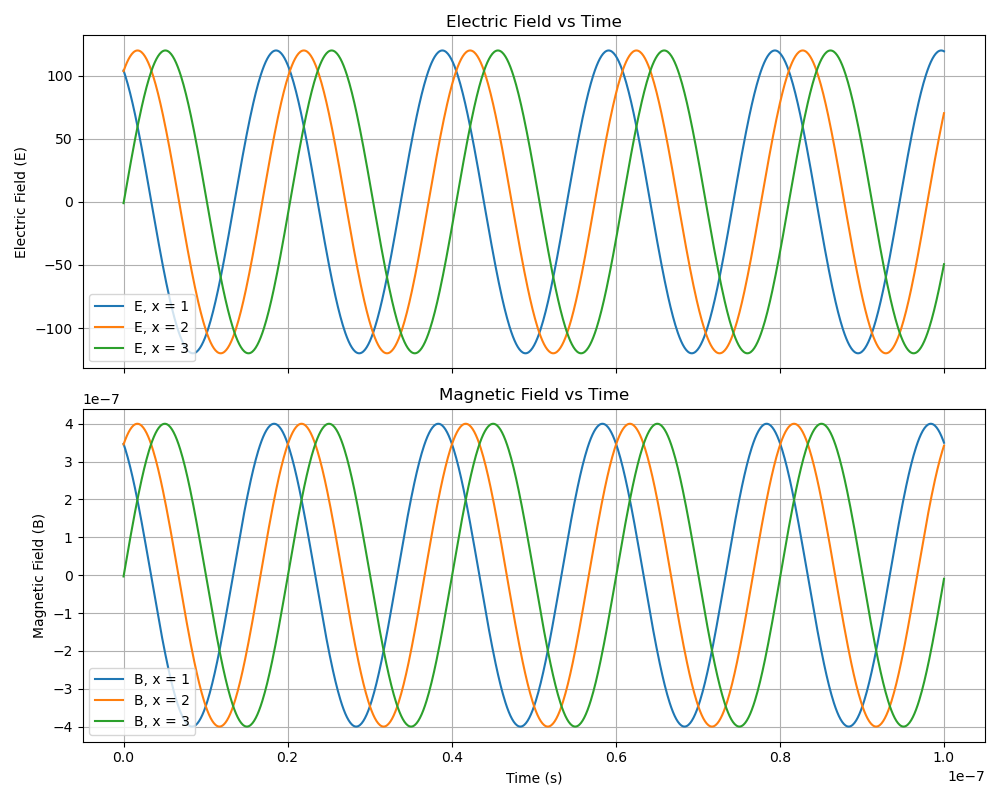
\includegraphics[width=1.05\columnwidth]{ncert-physics/12/8/8/figs/Figure_1.png}
  \label{fig:fig1.12.8.8}

\end{figure}

\end{flushleft}

%\end{document}


\pagebreak
\item A charged particle oscillates about its mean equilibrium position with a frequency of $10^9Hz$. What is the frequency of the electromagnetic waves produced by the oscillator? \\
\solution
\iffalse
\let\negmedspace\undefined
\let\negthickspace\undefined
\documentclass[journal,12pt,twocolumn]{IEEEtran}
\usepackage{cite}
\usepackage{amsmath,amssymb,amsfonts,amsthm}
\usepackage{algorithmic}
\usepackage{graphicx}
\usepackage{textcomp}
\usepackage{xcolor}
\usepackage{txfonts}
\usepackage{listings}
\usepackage{enumitem}
\usepackage{mathtools}
\usepackage{gensymb}
\usepackage{comment}
\usepackage[breaklinks=true]{hyperref}
\usepackage{tkz-euclide} 
\usepackage{listings}
\usepackage{gvv}                                        
\def\inputGnumericTable{}                                 
\usepackage[latin1]{inputenc}                                
\usepackage{color}                                            
\usepackage{array}                                            
\usepackage{longtable}                                       
\usepackage{calc}                                             
\usepackage{multirow}                                         
\usepackage{hhline}                                           
\usepackage{ifthen}                                           
\usepackage{lscape}
\usepackage[export]{adjustbox}

\newtheorem{theorem}{Theorem}[section]
\newtheorem{problem}{Problem}
\newtheorem{proposition}{Proposition}[section]
\newtheorem{lemma}{Lemma}[section]
\newtheorem{corollary}[theorem]{Corollary}
\newtheorem{example}{Example}[section]
\newtheorem{definition}[problem]{Definition}
\newcommand{\BEQA}{\begin{eqnarray}}
\newcommand{\EEQA}{\end{eqnarray}}
\newcommand{\define}{\stackrel{\triangle}{=}}
\theoremstyle{remark}
\newtheorem{rem}{Remark}
\begin{document}
\parindent 0px
\bibliographystyle{IEEEtran}

\title{Assignment\\[1ex]12.8 - 6}
\author{EE23BTECH11034 - Prabhat Kukunuri$^{}$% <-this % stops a space
}
\maketitle
\newpage
\bigskip

\renewcommand{\thefigure}{\theenumi}
\renewcommand{\thetable}{\theenumi}
\section*{Question}
A charged particle oscillates about its mean equilibrium position with a frequency of $10^9Hz$. What is the frequency of the electromagnetic waves produced by the oscillator?

\section*{Solution}
\fi
\begin{table}[h]
    \centering
    \begin{tabular}{|c|c|c|}
    \hline
   Symbol&Value&Description\\ \hline
   $y(t)$&$\cos\brak{2{\pi}f_ct}$&Wave equation of electro-magnetic wave\\ \hline
   $f_c$&$10^9$&Frequency of electromagnetic wave\\ \hline
   $t$&seconds&Time\\ \hline

    \end{tabular}
    \caption{Variable description}
    \label{tab:12.8.6.1}
\end{table}

\begin{figure}[h]
    \centering
    \includegraphics[width=\columnwidth]{Figure_1.png}
    \caption{$y(t)=\cos\brak{2{\pi}\times 10^9t}$}
    \label{fig:12.8.6.2}
\end{figure}
%\end{document}
\pagebreak
\item Given below are some functions of x and t to 
represent the displacement (transverse
or longitudinal) of an elastic wave. State which of these represents \brak i travelling
wave, \brak {ii} a stationary wave or \brak {iii} none at all: \\
\begin{enumerate}
\item $y = 2\cos \brak{3x} \sin \brak{10t}$
\item $y=2\sqrt{x-vt}$
\item $y = 3\sin \brak{5x - 0.5t} + 4\cos \brak{5x - 0.5t}$
\item $y = \cos x \sin t + \cos 2x \sin 2t$
\end{enumerate}
\solution
\iffalse
\let\negmedspace\undefined
\let\negthickspace\undefined
\documentclass[journal,12pt,twocolumn]{IEEEtran}
\usepackage{cite}
\usepackage{amsmath,amssymb,amsfonts,amsthm}
\usepackage{algorithmic}
\usepackage{graphicx}
\usepackage{textcomp}
\usepackage{xcolor}
\usepackage{txfonts}
\usepackage{listings}
\usepackage{enumitem}
\usepackage{mathtools}
\usepackage{gensymb}
\usepackage{comment}
\usepackage[breaklinks=true]{hyperref}
\usepackage{tkz-euclide} 
\usepackage{listings}
\usepackage{gvv}                                        
\def\inputGnumericTable{}                                 
\usepackage[latin1]{inputenc}                                
\usepackage{color}                                            
\usepackage{array}                                            
\usepackage{longtable}                                       
\usepackage{calc}                                             
\usepackage{multirow}                                         
\usepackage{hhline}                                           
\usepackage{ifthen}                                           
\usepackage{lscape}
\newtheorem{theorem}{Theorem}[section]
\newtheorem{problem}{Problem}
\newtheorem{proposition}{Proposition}[section]
\newtheorem{lemma}{Lemma}[section]
\newtheorem{corollary}[theorem]{Corollary}
\newtheorem{example}{Example}[section]
\newtheorem{definition}[problem]{Definition}
\newcommand{\BEQA}{\begin{eqnarray}}
\newcommand{\EEQA}{\end{eqnarray}}
\newcommand{\define}{\stackrel{\triangle}{=}}
\theoremstyle{remark}
\newtheorem{rem}{Remark}
\begin{document}
\parindent 0px
\bibliographystyle{IEEEtran}
\title{ASSIGNMENT11.15\_13Q}
\author{EE22BTECH11219 - Sai Sujan Rada$^{}$% <-this % stops a space
}
\maketitle
\newpage
\bigskip
\section*{QUESTION}
Given below are some functions of x and t to 
represent the displacement (transverse
or longitudinal) of an elastic wave. State which of these represents \brak i travelling
wave, \brak {ii} a stationary wave or \brak {iii} none at all: \\
\begin{enumerate}
\item $y = 2\cos \brak{3x} \sin \brak{10t}$
\item $y=2\sqrt{x-vt}$
\item $y = 3\sin \brak{5x - 0.5t} + 4\cos \brak{5x - 0.5t}$
\item $y = \cos x \sin t + \cos 2x \sin 2t$
\end{enumerate}
\solution 

\fi
\begin{table}[htbp]
    \centering
    \def\arraystretch{1.5}
    \begin{tabular}{|p{4cm}|p{4cm}|}
    \hline
TRAVELLING WAVE  & STATIONARY WAVE \\ \hline
    $y \brak{x,t} =A \sin  \brak{kx \pm \omega t} $ & $y\brak{ x,t }=A\sin kx\cos \omega t $ \\   \hline
    \hline
PARAMETERS  & DEFINITION  \\  \hline
$A$    &  Amplitude  \\ \hline
 $\omega$  & Angular Velocity  \\  \hline
 $x$    & Position  \\  \hline
 $k$    & Wavenumber    \\  \hline 
    \end{tabular}
    \caption{Travelling wave $vs$ Stationary wave}
    \label{tab:table11.15.13.1}
\end{table}

Let us assume an equation:
\begin{align}
y=A(x)\cos \brak{\omega t+\phi\brak {x}}
\end{align}
\begin{table}[htbp]
    \centering
    \def\arraystretch{1.5}
    \begin{tabular}{|p{4cm}|p{4cm}|}
    \hline
STATIONARY WAVE CONDITION & TRAVELLING WAVE CONDITION \\ \hline
        \brak 1 $A(x)$ should be a function of position x, and it can be expressed as $A(x)=A_{0}cos(\omega t+\alpha)$ where $A_{0}$ is a constant, $k$ is the wavenumber, $x$ is the position and $\alpha$ is a phase constant. & 
        \brak 1 $A(x)$ should be a constant, and it can be expressed as $A(x)=A_{0}$ where $A_{0}$ is a constant number. \\ \hline

        \brak 2 $\phi (x)$ can be expressed as $\phi (x)=c$ where c is a constant. &
        \brak 2 $\phi (x)$ represents a linear expression in x, and it can be expressed as $\phi (x)=kx+\theta$ where k is the wavenumber and $\theta$ is the phaseconstant. \\ \hline
\end{tabular}
    \caption{Travelling wave $vs$ Stationary wave}
    \label{tab:table1}
\end{table}

\begin{figure}[ht]
                        \centering
                        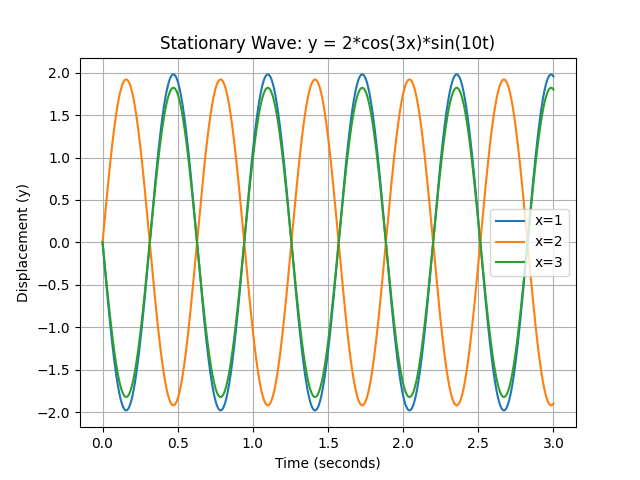
\includegraphics[width=\columnwidth]{figs/a.png}
                        \caption{DIPLACEMENT $vs$ TIME-graph1}
                        \label{fig:11.15.13.1}
\end{figure}
\begin{figure}[ht]
                            \centering
                            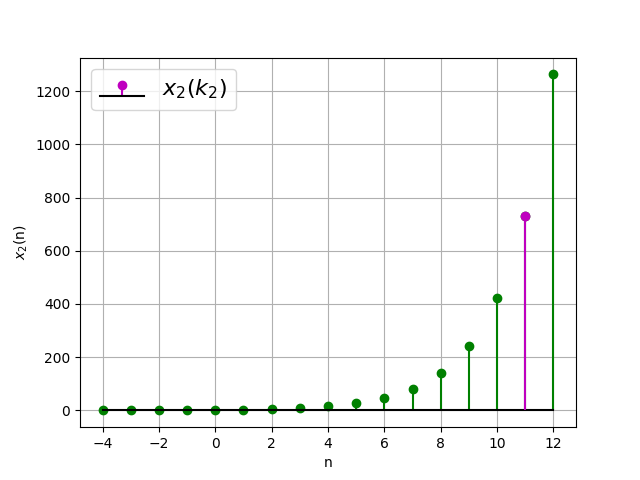
\includegraphics[width=\columnwidth]{figs/b.png}
                            \caption{DIPLACEMENT $vs$ TIME-graph2}
                            \label{fig:11.15.13.2}
\end{figure}   
\begin{figure}[ht]
                             \centering
                             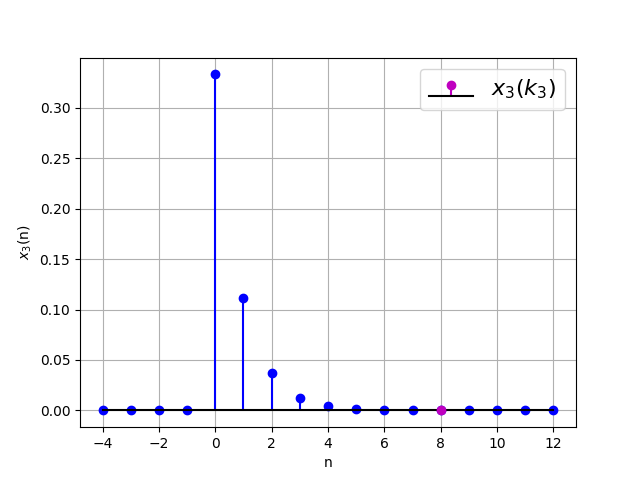
\includegraphics[width=\columnwidth]{figs/c.png}
                             \caption{DIPLACEMENT $vs$ TIME-graph3}
                             \label{fig:11.15.13.3}
\end{figure}
\begin{figure}[ht]
                            \centering
                            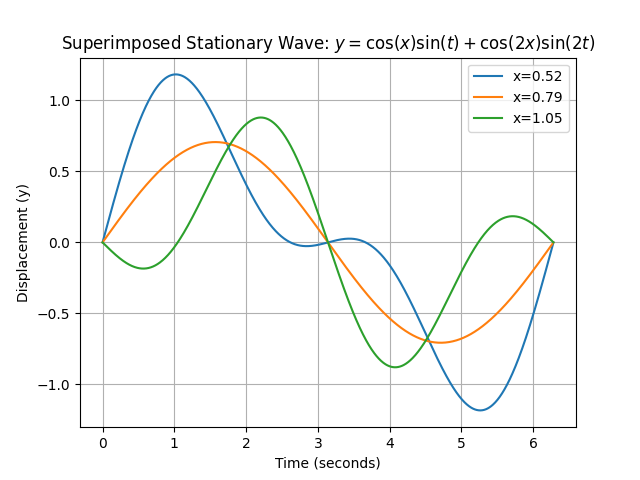
\includegraphics[width=\columnwidth]{figs/d.png}
                            \caption{DIPLACEMENT $vs$ TIME-graph4}
                            \label{fig:11.15.13.4}
\end{figure}
\figref{fig:11.15.13.1} and \figref{fig:11.15.13.3} are self explanatory for stationary and travelling waves.\figref{fig:11.15.13.2} and \figref{fig:11.15.13.4} are neither stationary nor travelling waves.


\pagebreak
\item For the travelling harmonic wave
$y\brak {x, t} = 2.0 \cos 2\pi \brak{10t - 0.0080 x + 0.35}$ where $x$ and $y$ are in $cm$ and $t$ in $s$. Calculate the phase difference between oscillatory
motion of two points separated by a distance of 

\begin{enumerate} [label=(\alph*)]
    \item $4 m$
    \item $0.5 m$
    \item $\lambda/2$
    \item $3\lambda/4$
\end{enumerate}
\solution
% \iffalse
\let\negmedspace\undefined
\let\negthickspace\undefined
\documentclass[journal,12pt,twocolumn]{IEEEtran}
\usepackage{cite}
\usepackage{amsmath,amssymb,amsfonts,amsthm}
\usepackage{algorithmic}
\usepackage{graphicx}
\usepackage{textcomp}
\usepackage{xcolor}
\usepackage{txfonts}
\usepackage{listings}
\usepackage{enumitem}
\usepackage{mathtools}
\usepackage{gensymb}
\usepackage{comment}
\usepackage[breaklinks=true]{hyperref}
\usepackage{tkz-euclide} 
\usepackage{listings}
\usepackage{gvv}                                        
\def\inputGnumericTable{}                                 
\usepackage[latin1]{inputenc}                               \usepackage{caption}
\usepackage{color}                                            
\usepackage{array}                                            
\usepackage{longtable}                                       
\usepackage{calc}                                             
\usepackage{multirow}                                         
\usepackage{hhline}                                           
\usepackage{ifthen}                                           
\usepackage{lscape}

\newtheorem{theorem}{Theorem}[section]
\newtheorem{problem}{Problem}
\newtheorem{proposition}{Proposition}[section]
\newtheorem{lemma}{Lemma}[section]
\newtheorem{corollary}[theorem]{Corollary}
\newtheorem{example}{Example}[section]
\newtheorem{definition}[problem]{Definition}
\newcommand{\BEQA}{\begin{eqnarray}}
\newcommand{\EEQA}{\end{eqnarray}}
\newcommand{\define}{\stackrel{\triangle}{=}}
\theoremstyle{remark}
\newtheorem{rem}{Remark}
\begin{document}

\bibliographystyle{IEEEtran}
\vspace{3cm}

\title{NCERT 11.15. Q10}
\author{EE23BTECH11010 - Venkatesh Bandawar$^{*}$% <-this % stops a space
}
\maketitle
\newpage
\bigskip

\renewcommand{\thefigure}{\arabic{figure}}
\renewcommand{\thetable}{\arabic{table}}

\bibliographystyle{IEEEtran}

\parindent 0px
\textbf{Question:} For the travelling harmonic wave
$y\brak {x, t} = 2.0 \cos 2\pi \brak{10t - 0.0080 x + 0.35}$ where $x$ and $y$ are in $cm$ and $t$ in $s$. Calculate the phase difference between oscillatory
motion of two points separated by a distance of 

\begin{enumerate} [label=(\alph*)]
    \item $4 m$
    \item $0.5 m$
    \item $\lambda/2$
    \item $3\lambda/4$
\end{enumerate}

\textbf{Solution:}  
\begin{table}[htbp] \small
\centering
\begin{table}[ht]
    \centering
    \begin{tabular}{|c|c|c|}
        \hline
        Parameter & Value & Description \\
        \hline
        $x(0)$ & 5 & First term of AP \\
        $d$ & 1.75 & Common difference of AP \\
        $x(n)$ & 20.75 & $n^{th}$ term of AP \\
        \hline
    \end{tabular}
    \vspace{2mm}
    \caption{Parameter List}
    \label{tab:simple.10.5.2.20}
\end{table}

\caption{Given \, parameters list}
\label{tab:given parameters list}
\end{table}
\begin{align}
    \brak{\Delta \theta} &= \brak{ 2\pi f t - kx_1 + \phi}  - \brak{2\pi f t -kx_2 + \phi}\\
    &= k\brak{x_2 - x_1} 
\end{align}

\begin{table}[htbp] 
\centering
\begin{tabular}{|c|c|c|}
        \hline
        \textbf{Parameter} & \textbf{Value} & \textbf{Description} \\
        \hline
        $x(0)$ & & First term \\
        \hline
        $r$ & & Common ratio \\
        \hline
        $x(0)^3r^3$ & 1 & Product of terms \\
        \hline
        $x(0)$ + $x(0)r$ + $x(0)r^2$ & $\frac{39}{10}$ & Sum of terms \\
        \hline
    \end{tabular}

\caption{Phase \, differences}
\label{tab:phase differences}
\end{table}

\begin{figure}[!h] 
\centering
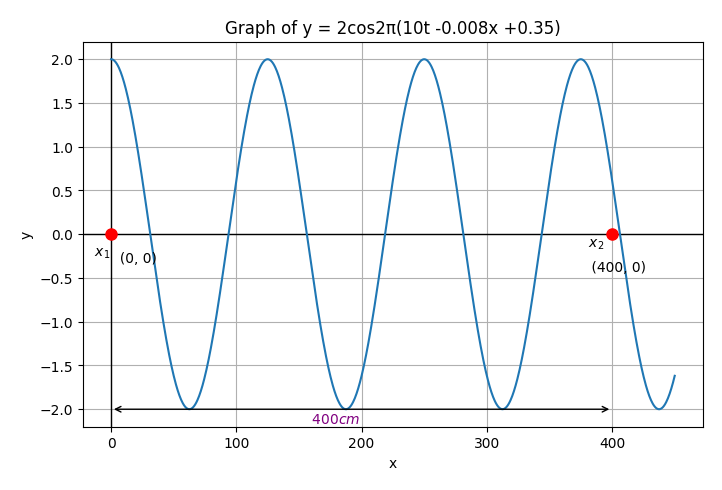
\includegraphics[width=\columnwidth]{figs/graph1.png}
\captionsetup{justification=centering}
\caption{}
\label{fig:Graph1}
\end{figure}

\begin{figure}[!h] 
\centering
\includegraphics[width=\columnwidth]{figs/graph2.png}
\captionsetup{justification=centering}
\caption{}
\label{fig:Graph2}
\end{figure}

\begin{figure}[!h] 
\centering
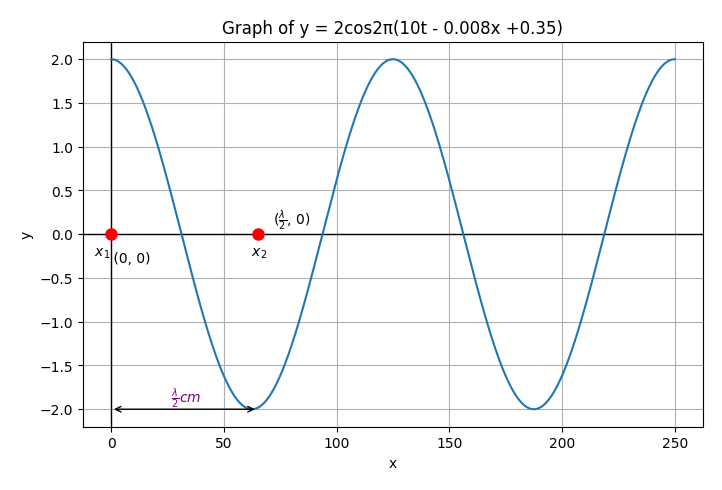
\includegraphics[width=\columnwidth]{figs/graph3.png}
\captionsetup{justification=centering}
\caption{}
\label{fig:Graph3}
\end{figure}

\begin{figure}[!h] 
\centering
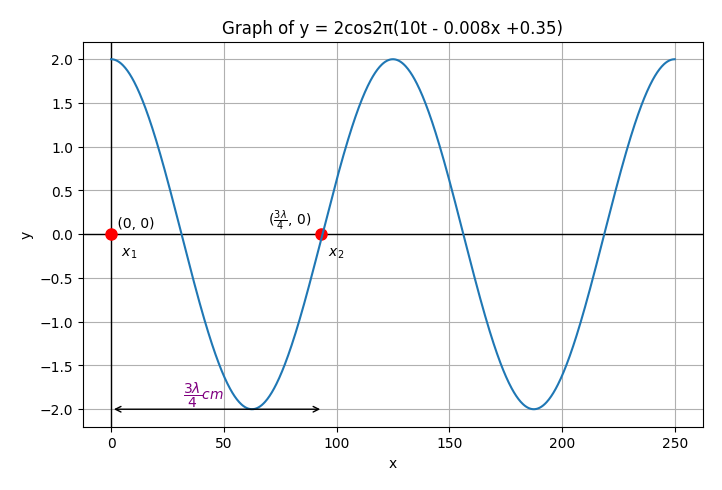
\includegraphics[width=\columnwidth]{figs/graph4.png}
\captionsetup{justification=centering}
\caption{}
\label{fig:Graph4}
\end{figure}



\end{document}

\pagebreak
\item 
\begin{enumerate}
\item The peak voltage of an AC supply is 300 V. What is the rms voltage?
\item The rms value of current in an AC circuit is 10 A. What is the peak current?
\end{enumerate}
\solution
\iffalse
\let\negmedspace\undefined
\let\negthickspace\undefined
\documentclass[journal,12pt,onecolumn]{IEEEtran}
\usepackage{cite}
\usepackage{amsmath,amssymb,amsfonts,amsthm}
%\usepackage{algorithmic}
\usepackage{graphicx}
\usepackage{textcomp}
usepackage{array}
\usepackage{xcolor}
\usepackage{txfonts}
\usepackage{listings}
\usepackage{enumitem}
\usepackage{mathtools}
\usepackage{gensymb}
\usepackage[breaklinks=true]{hyperref}
\usepackage{tkz-euclide} % loads  TikZ and tkz-base
\usepackage{listings}
\usepackage{float}



\newtheorem{theorem}{Theorem}[section]
\newtheorem{problem}{Problem}
\newtheorem{proposition}{Proposition}[section]
\newtheorem{lemma}{Lemma}[section]
\newtheorem{corollary}[theorem]{Corollary}
\newtheorem{example}{Example}[section]
\newtheorem{definition}[problem]{Definition}
%\newtheorem{thm}{Theorem}[section] 
%\newtheorem{defn}[thm]{Definition}
%\newtheorem{algorithm}{Algorithm}[section]
%\newtheorem{cor}{Corollary}
\newcommand{\BEQA}{\begin{eqnarray}}
\newcommand{\EEQA}{\end{eqnarray}}
\newcommand{\define}{\stackrel{\triangle}{=}}
\theoremstyle{remark}
\newtheorem{rem}{Remark}
%\bibliographystyle{ieeetr}
\begin{document}
%
\providecommand{\pr}[1]{\ensuremath{\Pr\left(#1\right)}}
\providecommand{\prt}[2]{\ensuremath{p_{#1}^{\left(#2\right)} }}        % own macro for this question
\providecommand{\qfunc}[1]{\ensuremath{Q\left(#1\right)}}
\providecommand{\sbrak}[1]{\ensuremath{{}\left[#1\right]}}
\providecommand{\lsbrak}[1]{\ensuremath{{}\left[#1\right.}}
\providecommand{\rsbrak}[1]{\ensuremath{{}\left.#1\right]}}
\providecommand{\brak}[1]{\ensuremath{\left(#1\right)}}
\providecommand{\lbrak}[1]{\ensuremath{\left(#1\right.}}
\providecommand{\rbrak}[1]{\ensuremath{\left.#1\right)}}
\providecommand{\cbrak}[1]{\ensuremath{\left\{#1\right\}}}
\providecommand{\lcbrak}[1]{\ensuremath{\left\{#1\right.}}
\providecommand{\rcbrak}[1]{\ensuremath{\left.#1\right\}}}
\newcommand{\sgn}{\mathop{\mathrm{sgn}}}
\providecommand{\abs}[1]{\left\vert#1\right\vert}
\providecommand{\res}[1]{\Res\displaylimits_{#1}} 
\providecommand{\norm}[1]{\left\lVert#1\right\rVert}
%\providecommand{\norm}[1]{\lVert#1\rVert}
\providecommand{\mtx}[1]{\mathbf{#1}}
\providecommand{\mean}[1]{E\left[ #1 \right]}
\providecommand{\cond}[2]{#1\middle|#2}
\providecommand{\fourier}{\overset{\mathcal{F}}{ \rightleftharpoons}}
\newenvironment{amatrix}[1]{%
  \left(\begin{array}{@{}*{#1}{c}|c@{}}
}{%
  \end{array}\right)
}
%\providecommand{\hilbert}{\overset{\mathcal{H}}{ \rightleftharpoons}}
%\providecommand{\system}{\overset{\mathcal{H}}{ \longleftrightarrow}}
	%\newcommand{\solution}[2]{\textbf{Solution:}{#1}}
\newcommand{\solution}{\noindent \textbf{Solution: }}
\newcommand{\cosec}{\,\text{cosec}\,}
\providecommand{\dec}[2]{\ensuremath{\overset{#1}{\underset{#2}{\gtrless}}}}
\newcommand{\myvec}[1]{\ensuremath{\begin{pmatrix}#1\end{pmatrix}}}
\newcommand{\mydet}[1]{\ensuremath{\begin{vmatrix}#1\end{vmatrix}}}
\newcommand{\myaugvec}[2]{\ensuremath{\begin{amatrix}{#1}#2\end{amatrix}}}
\providecommand{\rank}{\text{rank}}
\providecommand{\pr}[1]{\ensuremath{\Pr\left(#1\right)}}
\providecommand{\qfunc}[1]{\ensuremath{Q\left(#1\right)}}
	\newcommand*{\permcomb}[4][0mu]{{{}^{#3}\mkern#1#2_{#4}}}
\newcommand*{\perm}[1][-3mu]{\permcomb[#1]{P}}
\newcommand*{\comb}[1][-1mu]{\permcomb[#1]{C}}
\providecommand{\qfunc}[1]{\ensuremath{Q\left(#1\right)}}
\providecommand{\gauss}[2]{\mathcal{N}\ensuremath{\left(#1,#2\right)}}
\providecommand{\diff}[2]{\ensuremath{\frac{d{#1}}{d{#2}}}}
\providecommand{\myceil}[1]{\left \lceil #1 \right \rceil }
\newcommand\figref{Fig.~\ref}
\newcommand\tabref{Table~\ref}
\newcommand{\sinc}{\,\text{sinc}\,}
\newcommand{\rect}{\,\text{rect}\,}
%%
%	%\newcommand{\solution}[2]{\textbf{Solution:}{#1}}
%\newcommand{\solution}{\noindent \textbf{Solution: }}
%\newcommand{\cosec}{\,\text{cosec}\,}
%\numberwithin{equation}{section}
%\numberwithin{equation}{subsection}
%\numberwithin{problem}{section}
%\numberwithin{definition}{section}
%\makeatletter
%\@addtoreset{figure}{problem}
%\makeatother

%\let\StandardTheFigure\thefigure
\let\vec\mathbf

\bibliographystyle{IEEEtran}





\bigskip

%\renewcommand{\thefigure}{\theenumi}
%\renewcommand{\thetable}{\theenumi}
%\renewcommand{\theequation}{\theenumi}

Q: \\
\begin{enumerate}
\item The peak voltage of an AC supply is 300 V. What is the rms voltage?
\item The rms value of current in an AC circuit is 10 A. What is the peak current?
\end{enumerate}

\solution
\fi

\begin{table}
\centering
  \begin{tabular}{|c|c|c|}
    \hline
    parameter & value & description \\
    \hline
    $V(t)$ & $V_{\text{0}} \cdot \sin(2\pi ft + \phi)$ & voltage in terms of time \\
    \hline
    $I(t)$ & $I_{\text{0}} \cdot \sin(2\pi ft + \phi)$ & current in terms of time \\
    \hline
    $V_0$ & $300 \, \text{V}$ & peak voltage \\
    \hline
    $V_ \text{rms}$ & $\sqrt{\frac{1}{T} \int_{0}^{T} [V(t)]^2 \, dt}$ & rms value of Voltage \\
    \hline 
    $I_ \text{rms}$ & $10 \, \text{A}$ & rms value of current\\
    \hline
    $I_0$ & $\sqrt{2} \times I_{\text{rms}}$ & peak current \\
    \hline
    $f$ & $50 \, \text{Hz}$ & frequence of the sinosoidal wave. \\
    \hline
    $T$ & $0.02 \, \text{s}$ & time period of sinosoidal wave. \\
    \hline
  \end{tabular}

\caption{Input Parameter Table}
\label{tab:input_parameters}
\end{table}
  


\begin{enumerate}
\item
\begin{align}
V_{\text{rms}}^2 &= {\frac{1}{T} \int_{0}^{T} [V(t)]^2 \, dt} \\
&= {f \int_{0}^{\frac{1}{f}} V_{\text{0}}^2 \cdot \sin^2(2\pi ft + \phi) \, dt} \\
&= \frac{1}{2} V_{0}^2 \left(1 - \frac{1}{f}\int_{0}^{\frac{1}{f}} \cos(4\pi ft + 2\phi) \, dt \right) \\
&= \frac{1}{2} V_{0}^2 \left(1 - \frac{1}{f}\left[\frac{\sin(4\pi ft + 2\phi)}{4\pi f}\right]_{0}^{\frac{1}{f}}\right) \\
&= \frac{1}{2} V_{0}^2 \left(1 - \frac{1}{f} \cdot \frac{\sin\left(4\pi + 2\phi\right) - \sin(0 + 2\phi)}{4\pi f}\right) \\
V_{\text{rms}} &= \frac{V_{0}}{\sqrt{2}} \label{eq:12.7.2_voltage}
\end{align}

To find the RMS voltage (\(V_{\text{rms}})\) when the peak voltage (\(V_{\text{0}})\) is 300V, you can use equation  \eqref{eq:12.7.2_voltage}

\begin{align}
V_{\text{rms}} &= \frac{300V}{\sqrt{2}} \approx 212.13V
\end{align}

\item 
\begin{align}
I_{\text{rms}}^2 &= {\frac{1}{T} \int_{0}^{T} [I(t)]^2 \, dt} \\
&= {f \int_{0}^{\frac{1}{f}} I_{\text{0}}^2 \cdot \sin^2(2\pi ft + \phi) \, dt} \\
&= \frac{1}{2} I_{0}^2 \left(1 - \frac{1}{f}\left[\frac{\sin(4\pi ft + 2\phi)}{4\pi f}\right]_{0}^{\frac{1}{f}}\right) \\
&= \frac{1}{2} I_{0}^2 \left(1 - \frac{1}{f} \cdot \frac{\sin\left(4\pi + 2\phi\right) - \sin(0 + 2\phi)}{4\pi f}\right) \\
I_{\text{rms}} &= \frac{I_{0}}{\sqrt{2}} \label{eq:12.7.2_current}
\end{align}

To find the peak current (\(I_{\text{0}}\)) when the RMS current (\(I_{\text{rms}}\)) is given, you can use equation  \eqref{eq:12.7.2_current}

\begin{align}
I_{\text{0}} \approx 10 \, \text{A} \times 1.414 \approx 14.14 \, \text{A}  
\end{align}

\begin{figure}[H]
    \centering
    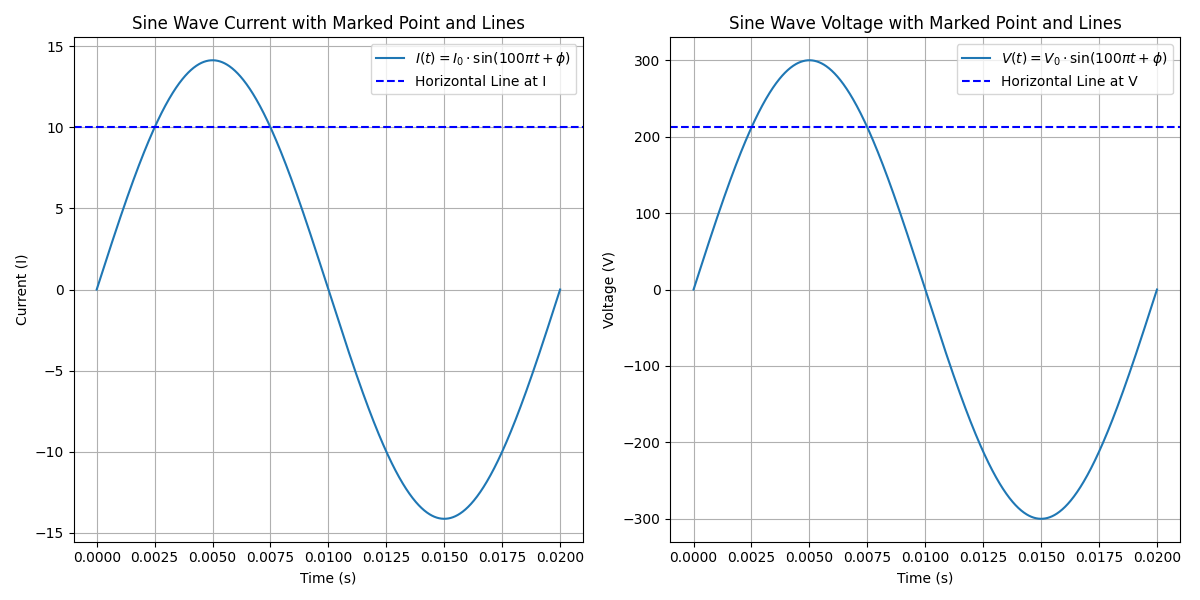
\includegraphics[width=\columnwidth]{.figs/merged_sine_wave_plots.png}

\end{enumerate}


\pagebreak
\item In Young’s double-slit experiment using monochromatic light of wavelength $\lambda$, the intensity of light at a point on the screen where path difference is $\lambda$, is $K$ units. What is the intensity of light at a
point where path difference is $\lambda$/3?\\

\solution

% \iffalse
\let\negmedspace\undefined
\let\negthickspace\undefined
\documentclass[journal,12pt,twocolumn]{IEEEtran}
\usepackage{cite}
\usepackage{amsmath,amssymb,amsfonts,amsthm}
\usepackage{algorithmic}
\usepackage{graphicx}
\usepackage{textcomp}
\usepackage{xcolor}
\usepackage{txfonts}
\usepackage{listings}
\usepackage{enumitem}
\usepackage{mathtools}
\usepackage{gensymb}
\usepackage{comment}
\usepackage[breaklinks=true]{hyperref}
\usepackage{tkz-euclide} 
\usepackage{listings}
\usepackage{gvv} 
\usepackage{caption}
\def\inputGnumericTable{}                                 
%\usepackage[latin1]{inputenc}                                
\usepackage{color}                                            
\usepackage{array}                                            
\usepackage{longtable}                                       
\usepackage{calc}                                             
\usepackage{multirow}                                         
\usepackage{hhline}                                           
\usepackage{ifthen}                                           
\usepackage{lscape}

\newtheorem{theorem}{Theorem}[section]
\newtheorem{problem}{Problem}
\newtheorem{proposition}{Proposition}[section]
\newtheorem{lemma}{Lemma}[section]
\newtheorem{corollary}[theorem]{Corollary}
\newtheorem{example}{Example}[section]
\newtheorem{definition}[problem]{Definition}
\newcommand{\BEQA}{\begin{eqnarray}}
\newcommand{\EEQA}{\end{eqnarray}}
\newcommand{\define}{\stackrel{\triangle}{=}}
\theoremstyle{remark}
\newtheorem{rem}{Remark}

\begin{document}

\bibliographystyle{IEEEtran}
\vspace{3cm}

\title{NCERT 12.10 5Q}
\author{EE23BTECH11013 - Avyaaz$^{*}$% <-this % stops a space 
}
\maketitle
\newpage
\bigskip

\renewcommand{\thefigure}{\arabic{figure}}
\renewcommand{\thetable}{\arabic{table}}

\large\textbf{\textsl{Question:}}
In Young’s double-slit experiment using monochromatic light of wavelength $\lambda$, the intensity of light at a point on the screen where path difference is $\lambda$, is $K$ units. What is the intensity of light at a
point where path difference is $\lambda$/3?\\
\large\textbf{\textsl{Solution:}}
\begin{table}[htbp]
\setlength{\extrarowheight}{8pt}
\centering
\begin{table}[h]
\renewcommand\thetable{1}
    \centering
    \begin{tabular}{|c|c|c|}
        \hline
        \textbf{Parameter} & \textbf{Description} & \textbf{Value}\\
        \hline
        $x(0)$ & First term & $2$\\
        \hline
        $x(19)$ & $20\textsuperscript{th}$ term & $-112$\\
        \hline
        $y(n)$ & sum upto $n\textsuperscript{th}$ term & \\
        \hline
    \end{tabular}
    \caption{Input data}
  \label{input data}
\end{table}

\caption{Parameters}
\label{tab:parameters}
\end{table}

From \tabref{tab:parameters}:
\begin{align}
%%y\brak{t} &= y_1\brak{t} + y_2\brak{t}  \\
y\brak{t} &= A\sin({2\pi f t - kx_1})  + A\sin({ 2\pi f t - kx_2}) \\
y\brak{t} &=  2A\cos\left(\dfrac{k\Delta x}{2}\right)\sin\left(2\pi f t - \dfrac{k(x_1+x_2)}{2} \right) \label{eq:superposition}
\end{align}
From \tabref{tab:parameters} and equation \eqref{eq:superposition}: 
\begin{align}
\therefore I \propto 4A^2\cos^2\left(\dfrac{k\Delta x}{2}\right)  \label{eq:intensity}
\end{align}
From \tabref{tab:parameters} and equation \eqref{eq:intensity}: 
\begin{align}
 \dfrac{K}{I_r} = \dfrac{4A^2\cos^2\left(\dfrac{2\pi}{2}\right)}{4A^2\cos^2\left(\dfrac{\pi}{3}\right)}
 \implies I_r = \dfrac{K}{4}
 \end{align}
 Hence, the Intensity of light at a point where path difference is $\dfrac{\lambda}{3}$ is $\dfrac{K}{4}$ units.

\begin{table}[htbp]
\centering
\begin{table}[ht]
    \centering
    \begin{tabular}{|c|c|c|}
        \hline
        Parameter & Value & Description \\
        \hline
        $x(0)$ & 5 & First term of AP \\
        $d$ & 1.75 & Common difference of AP \\
        $x(n)$ & 20.75 & $n^{th}$ term of AP \\
        \hline
    \end{tabular}
    \vspace{2mm}
    \caption{Parameter List}
    \label{tab:simple.10.5.2.20}
\end{table}

\caption{}
\label{tab:intensity}
\end{table}
Assuming $\Delta x= r\lambda$, 

From equation \eqref{eq:intensity}:
\begin{figure}[htbp]
    \centering
    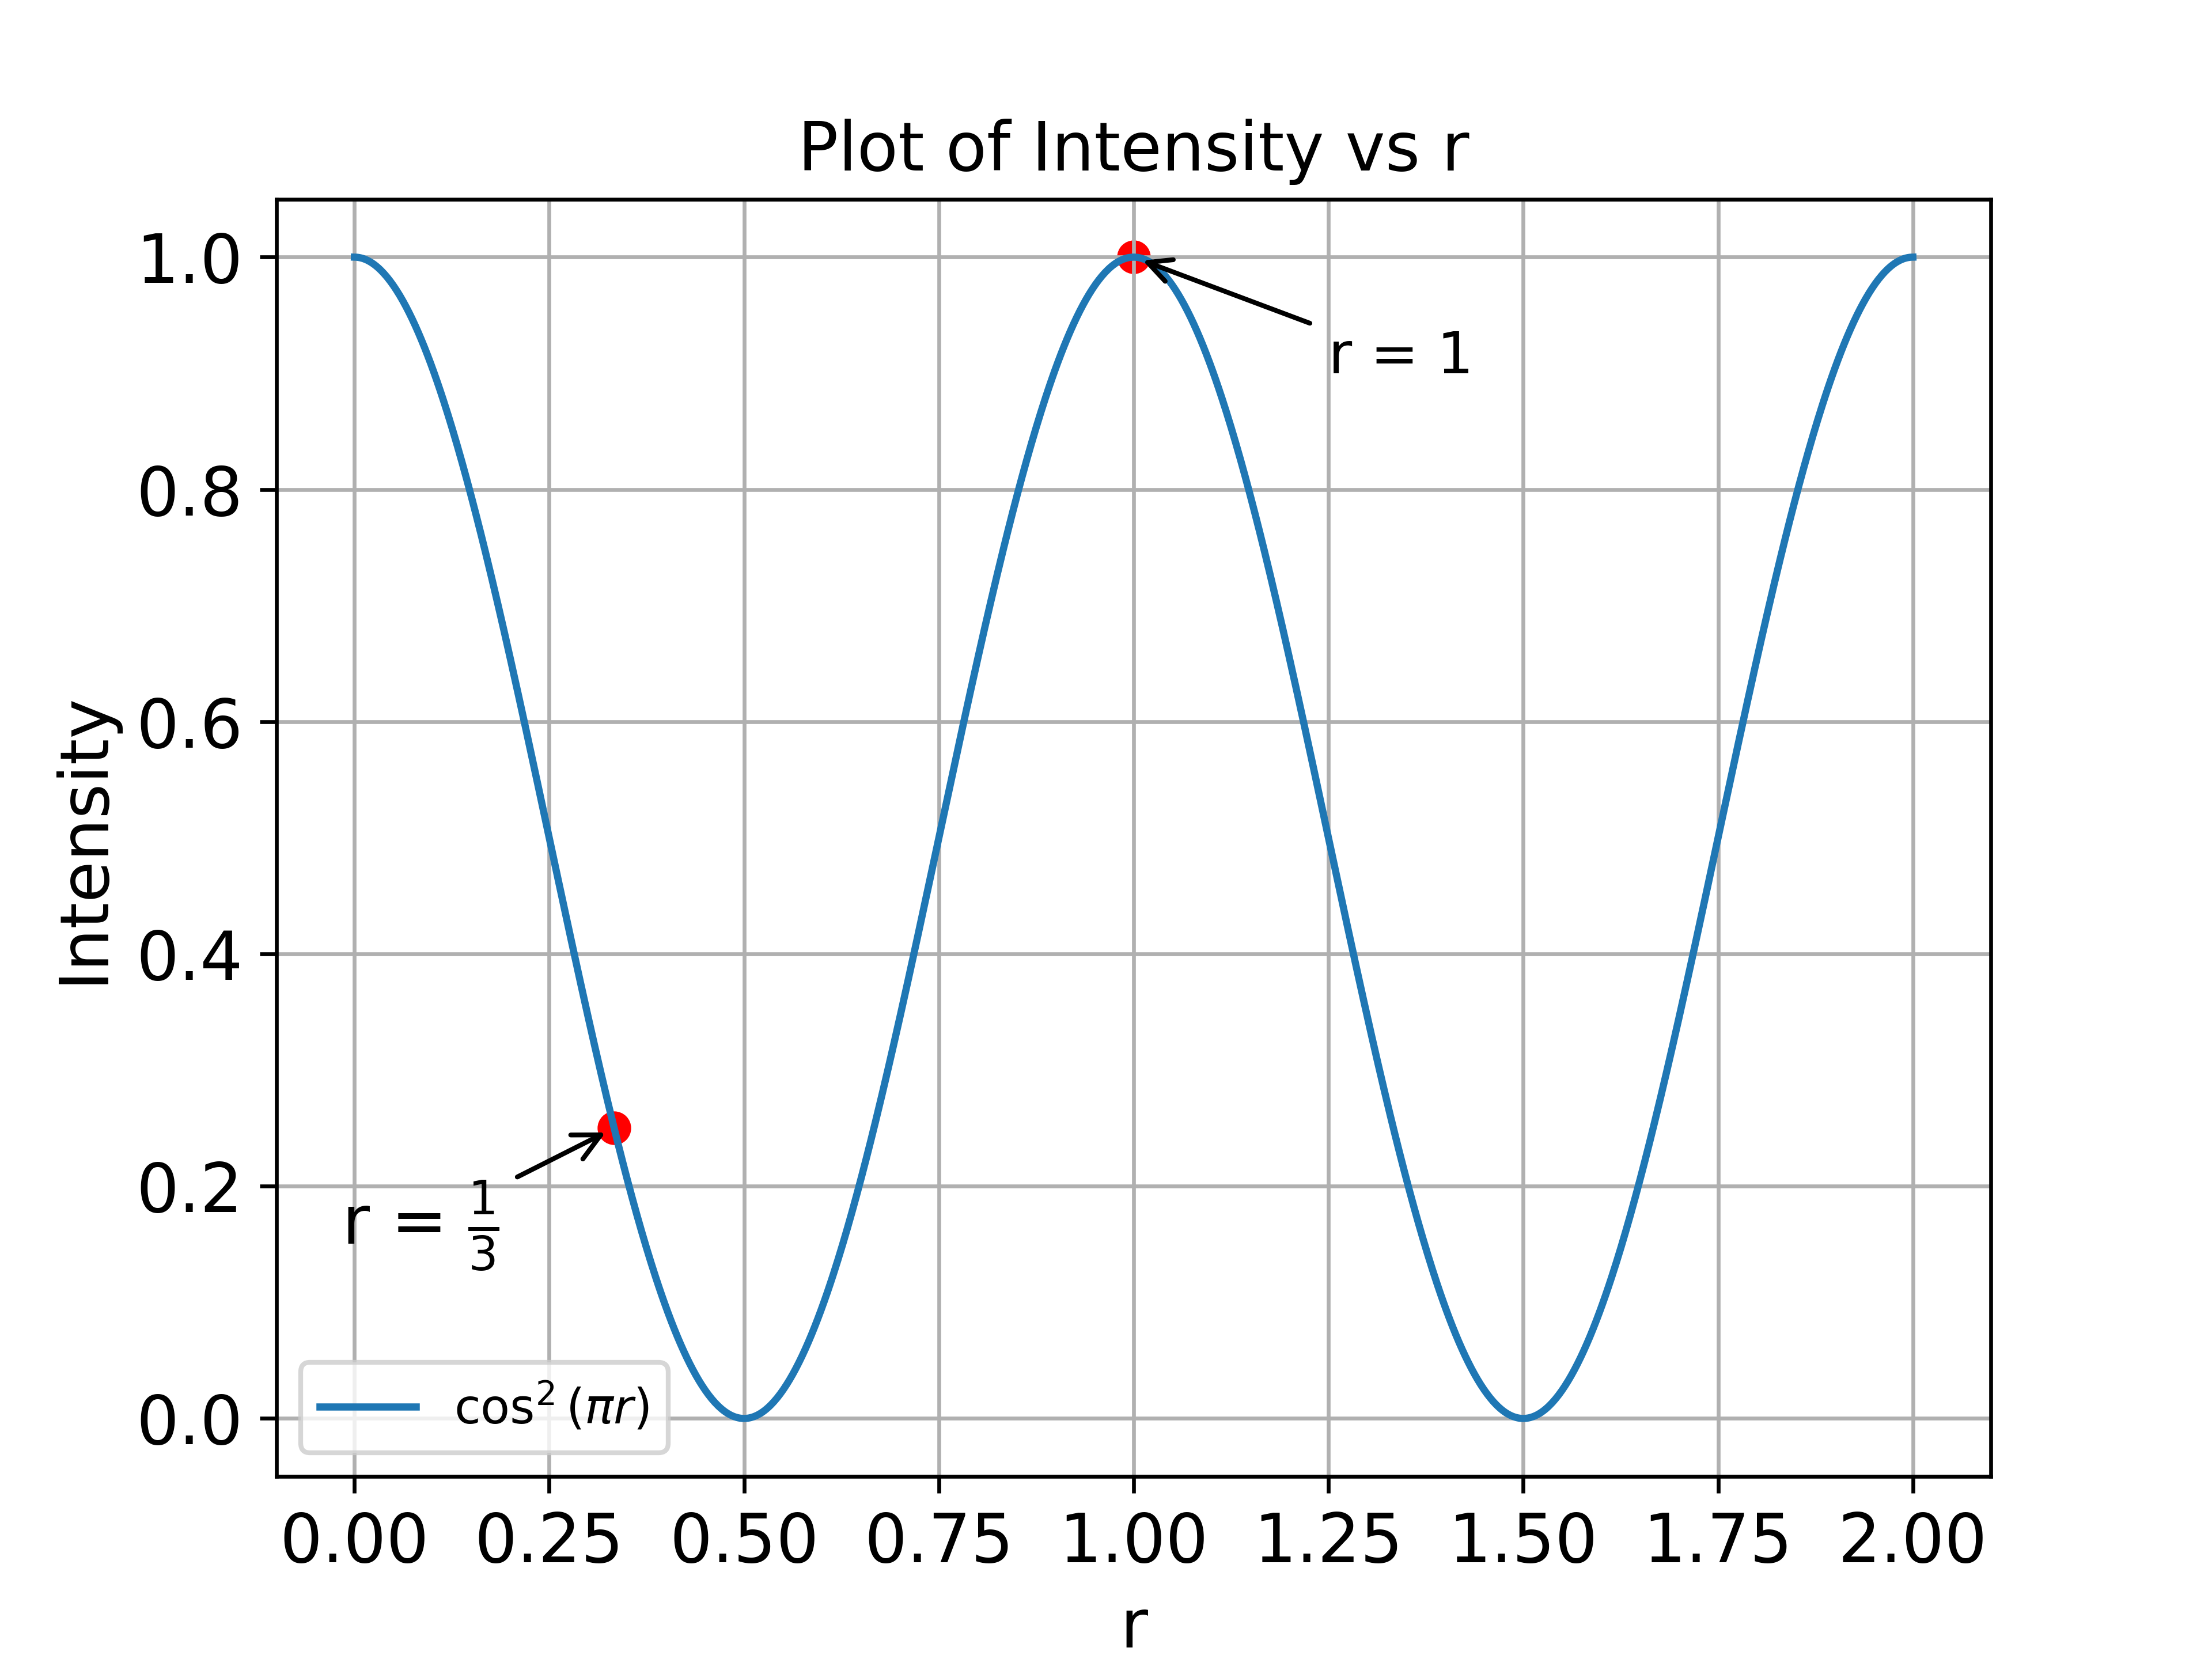
\includegraphics[width = \columnwidth]{figs/intensity_plot.png}
  \caption{}
    \label{fig:graph1}
\end{figure}
\bibliographystyle{IEEEtran}
\end{document}

\pagebreak

\item In a plane electromagnetic wave, the electric field oscillates sinusoidally at a frequency of $2.0 \text{ x } 10^{10}$ Hz and amplitude 48 $Vm^{-1}$.
\begin{enumerate}[label=(\alph*)]
    \item What is the wavelength of the wave?
    \item What is the amplitude of the oscillating magnetic field?
    \item Show that the average energy density of the $\vec{E}$ field equals the
average energy density of the $\vec{B}$ field. $[c = 3 \text{ x } 10^{8}ms^{-1} ]$
\end{enumerate}

\item \begin{enumerate}
\item For the wave on the string $y(x, t) = 0.06 \sin(\frac{2\pi x}{3}) \cos(120\pi t)$ , do all the points on the string     oscillate with the same (a)frequency , (b)phase , (c)amplitude ? Explain your answers. \\

 \item What is the amplitude of a point 0.375m away from one end? \\
 \end{enumerate}
 \solution
 \pagebreak
 
 \item 
 A transverse harmonic wave on a string is described by
\begin{align}
    y\brak{x,t}=3.0 \sin\brak{36t+0.018x+\frac{\pi}{4}}
\end{align}
where $x$ and $y$ are in cm and $t$ in s. The positive direction of $x$ is from left to right.
\begin{enumerate}[label=(\alph*)]
    \item Is this a travelling wave or a stationary wave? If it is travelling, what are the speed and direction of its propogation?
    \item What are its amplitude and frequency?
    \item What is the initial phase at the origin?
    \item  What is the least distance between two succesive crests in the wave?
\end{enumerate}

\solution
\pagebreak

\item In deriving the single slit diffraction pattern, it was stated that the intensity is zero at angles of $\frac{n\lambda}{a}$. Justify this by suitably dividing the slit to bring out the cancellation.\\
\solution
\pagebreak

\item A 60 $\mu$ F capacitor is connected to a 110 V, 60 Hz ac supply. Determine the rms value of the current in the circuit.\\
\solution
\pagebreak

\item A charged  $30\mu F$ capacitor is connected to a $27 mH$ inductor. What is the angular frequency of free oscillations of the circuit?\\
\solution
\pagebreak
\item Obtain the resonance frequency of a series LCR circuit with $L = 2.0\, H$, $C = 32\, \mu F$, and $R = 10\, \Omega$. What is the Q-value of the circuit.\\
\solution
\pagebreak
\item A charged 30 $\mu$F capacitor is connected to a 27 mH inductor. Suppose the initial charge on the capacitor is 6mC.What is the total energy stored in the circuit initially? What is the
total energy at later time? \\
\solution
\pagebreak

\item A wire stretched between two rigid supports vibrates in its fundamental mode with a frequency of $45 \, \text{Hz}$. The mass of the wire is $3.5 \times 10^{-2} \, \text{kg}$, and its linear mass density is $4.0 \times 10^{-2} \, \text{kg/m}$. The length of the wire is $0.875 \, \text{m}$. Determine the speed of a transverse wave on the string and the tension in the string.\\
\solution
\pagebreak

\item The given figure shows a series LCR circuit connected to a variable
frequency 230 V source. \\
L = 5.0 H, C = 80 $\mu$F, R = 40 $\Omega$.

\begin{figure}[h!]
\begin{center}
\begin{circuitikz}[american voltages]
      \draw (0,0)
      to[sV, l=$\varepsilon$] (0,2) 
      to[R, l=$R$, v=$V_R$] (4,2) 
      to[C, l=$C$, v=$V_C$] (4,0)
      to[L, l=$L$, v=$V_L$] (0,0);
\end{circuitikz}
\end{center}
\end{figure}

\begin{enumerate}
    \item Determine the source frequency which drives the circuit in resonance.
    \item Obtain the impedance of the circuit and the amplitude of current
at the resonating frequency.
    \item Determine the rms potential drops across the three elements of
the circuit. Show that the potential drop across the LC
combination is zero at the resonating frequency.\\
\end{enumerate}
\solution
\pagebreak

\item Q23) A narrow sound pulse (for example, a short pip by a whistle) is sent across a
	medium.\\ \brak{\text{a}} Does the pulse have a definite \brak{\text{i}} frequency, \brak{\text{ii}} wavelength, \brak{\text{iii}} speed
	of propagation?\\[1ex]\brak{\text{b}} If the pulse rate is 1 after every 20 s, (that is the whistle is
	blown for a split of second after every 20 s), Is the frequency of note produced
	by whistle equal to 1/20 or 0.05 Hz ?\\
\solution
\pagebreak
\item Suppose that the electric field part of an electromagnetic wave in vacuum given as\\ \textbf{E} =\{(3.1N/C)cos[(1.8 rad/m)y+(5.4$\times$10$^{6}$rad/s)t]\}\^i \\
(a) What is the direction of propagation ?\\
(b) What is the wavelength ? \\
(c) What is the frequency ?\\
(d) What is the amplitude of the magnetic field part of the wave?\\
(e) Write an expression for the magnetic field part of the wave.\\
\solution
\pagebreak

\item A 44 mH inductor is connected to 220 V, 50 Hz ac supply. Determine
the rms value of the current in the circuit.\\
\solution
\pagebreak

\item The 6563 \AA\, H$\alpha$ line emitted by hydrogen in a star is found to be redshifted by 15 \AA. Estimate the speed with which the star is receding from the Earth.
\solution
\pagebreak
\item The amplitude  of the magnetic part of a harmonic elctromagnetic wave is $B_0=510$nT.What is the amplitude of the electric part of the electromagnetic wave.\\
\solution
\pagebreak

\item A 100$\mu$F capacitor in series with a 40$\Omega$ resistance is connected to a 110V, 60Hz supply.
\begin{enumerate}[label = {\brak{\alph*}}]
\item What is the maximum current in the circuit?
\item What is the time lag between the current maximum and the voltage maximum?\\
\end{enumerate}
\solution
\pagebreak
\item A 100 $\ohm$ resistor is connected to $220 V$, $50 Hz$ AC supply.\\
(1) What is the rms value of current in the circuit?\\
(2) What is the net power consumed over a full cycle?

\solution
\pagebreak
\item  Two towers on top of two hills are $40$ km apart.This line joining them passes $50$ m above a hill halfway between the towers.What is the longest wavelength of radio waves,which can be sent between the towers without  appereciable diffraction effects?\\
\solution
\pagebreak
\item A circuit containing a 80mH inductor and a 60$\mu$F capacitor in series is connected to a 230V, 50Hz supply. The resistance of the circuit is negligible.\\
\begin{enumerate}
  \item Obtain the current amplitude and rms value.
  \item Obtain the rms value of potential drops across each element.
  \item What is the average power transferred to the inductor ?
  \item What is the average power transferred to the capacitor ?
  \item What is the total average power absorbed by the circuit ? \brak{\text{'Average' implies 'averaged over one cycle'.}}
\end{enumerate}
\solution
\pagebreak
\item A coil of inductance 0.50 H and resistance 100 $\Omega$ is connected to a 240 V, 50 Hz ac supply.\\
(a) What is the maximum current in the coil?\\		
(b) What is the time lag between the voltage maximum and the current maximum?\\
\solution
\pagebreak

\end{enumerate}

\chapter{Filters}
\begin{enumerate}[label=\thesection.\arabic*,ref=\thesection.\theenumi]
\item An LC circuit contains a $50 \mu H$ inductor and a $50 \mu F$ capacitor with an initial charge of $10 mC$. The resistance of the circuit is negligible. Let the instant the circuit is closed by $t = 0$.

\textbf{a)} What is the total energy stored initially? Is it conserved during LC oscillations?

\textbf{b)} What is the natural frequency of the circuit?

\textbf{c)} At what time is the energy stored \textbf{(i)} completely electrical (i.e., stored in the capacitor)? \textbf{(ii)} completely magnetic (i.e., stored in the inductor)?

\textbf{d)} At what times is the total energy shared equally between the inductor and the capacitor?

\textbf{e)} If a resistor is inserted in the circuit, how much energy is eventually dissipated as heat? \\
\hfill(NCERT-Physics 12.7 12Q)\\
\solution 
\pagebreak 

\item Obtain the resonant frequency and Q-factor of a series LCR circuit with $L = 3.0\, H$, $C = 27\, \mu F$, and $R = 7.4\, \Omega$. It is desired to improve the sharpness of the resonance of the circuit by reducing its `full width at half maximum' by a factor of 2. Suggest a suitable way.\\
\solution
\iffalse
\let\negmedspace\undefined
\let\negthickspace\undefined
\documentclass[journal,12pt,twocolumn]{IEEEtran}
\usepackage{cite}
\usepackage{amsmath,amssymb,amsfonts,amsthm}
\usepackage{algorithmic}
\usepackage{graphicx}
\usepackage{textcomp}
\usepackage{xcolor}
\usepackage{txfonts}
\usepackage{listings}
\usepackage{enumitem}
\usepackage{mathtools}
\usepackage{gensymb}
\usepackage{comment}
\usepackage[breaklinks=true]{hyperref}
\usepackage{tkz-euclide} 
\usepackage{listings}
\usepackage{gvv}  
\usepackage{tikz}
\usepackage{circuitikz} 
\usepackage{caption}
\def\inputGnumericTable{}              
\usepackage[latin1]{inputenc}          
\usepackage{color}                    
\usepackage{array}                     
\usepackage{longtable}                 
\usepackage{calc}                     \usepackage{multirow}                  
\usepackage{hhline}                    
\usepackage{ifthen}                    
\usepackage{lscape}
\usepackage{amsmath}
\newtheorem{theorem}{Theorem}[section]
\newtheorem{problem}{Problem}
\newtheorem{proposition}{Proposition}[section]
\newtheorem{lemma}{Lemma}[section]
\newtheorem{corollary}[theorem]{Corollary}
\newtheorem{example}{Example}[section]
\newtheorem{definition}[problem]{Definition}
\newcommand{\BEQA}{\begin{eqnarray}}
\newcommand{\EEQA}{\end{eqnarray}}
\newcommand{\define}{\stackrel{\triangle}{=}}
\theoremstyle{remark}
\newtheorem{rem}{Remark}

\begin{document}

\bibliographystyle{IEEEtran}
\vspace{3cm}

\title{NCERT Physics 12.7 Q21}
\author{EE23BTECH11009 - AROSHISH PRADHAN$^{*}$% <-this % stops a space
}
\maketitle
\newpage
\bigskip
\textbf{Question:} 
Obtain the resonant frequency and Q-factor of a series LCR circuit with $L = 3.0\, H$, $C = 27\, \mu F$, and $R = 7.4\, \Omega$. It is desired to improve the sharpness of the resonance of the circuit by reducing its `full width at half maximum' by a factor of 2. Suggest a suitable way.\\

\solution
\fi
Given parameters are:
\begin{table}[!h]
    \centering
    \resizebox{\columnwidth}{!}{
    \begin{tabular}{|c|c|c|}
    \hline
     \textbf{Symbol} & \textbf{Value} &
     \textbf{Description}\\
    \hline
     $L$ &  $3.0\,
     \text{H}$ & Inductance\\
    \hline 
     $C$ &  $27\, \mu\text{F}$ & Capacitance \\
    \hline
     R &  $7.4\, \Omega$ & Resistance\\
    \hline
     Q &  & \parbox{5cm}{Quality Factor: ratio of voltage across inductor or capacitor to that across the resistor at resonance}\\[8pt]
    \hline
     $\omega_0$ & $\dfrac{1}{\sqrt{LC}}$ & Angular Resonant Frequency\\[8pt]
    \hline
\end{tabular}
}
    \vspace{6 pt}
    \caption{Given Parameters}
    \label{tab:1}
\end{table}
\begin{figure}[!h]
 \centering
    \begin{circuitikz}
    \draw(0, 0) -- (1, 0);
    \draw(1, 0) to [L, l = $3.0\text{H}$](2, 0);
    \draw(2, 0) -- (3, 0);
    \draw(3, 0) to [C, l = $27\, \mu\text{F}$](4, 0);
    \draw(4, 0) -- (5, 0);
    \draw(5, 0) to [R, l = $7.4\Omega$](6, 0);
    \draw(0, 0) -- (0, -2);
    \draw[->] (0, -1) node[left] {$I(t)$} -- (0, -1);
    \draw(6, 0) -- (7, 0);
    \draw(7, 0) -- (7, -2);
    \draw(0, -2) -- (3, -2);
    \draw(7, -2) -- (7, -2);
    \draw(3, -2) to [sV, l = $V(t)$](4, -2);
    \draw(4, -2) -- (7, -2);
\end{circuitikz}

    \caption{LCR Circuit}
    \label{fig:enter-label}
\end{figure}
\begin{enumerate}
\item {Frequency Response of the Circuit}

From Kirchhoff's Voltage Law (KVL):
\begin{equation}
V(t) = V_R + V_L + V_C \label{eq:KVL}
\end{equation}
Using reactances from \figref{fig:2},
\begin{align}
    V(s) &= R I(s) + sL I(s) + \dfrac{1}{sC} I(s)\\
    &= I(s)\left(R + Ls + \dfrac{1}{sC}\right)\\
    \implies I(s) &= \dfrac{V(s)}{\left(R + Ls + \dfrac{1}{sC}\right)} \label{eq: 4}
\end{align}
\begin{figure}[!h]
 \centering
    \begin{circuitikz}
    \draw(0, 0) -- (1, 0);
    \draw(1, 0) to [L, l = $sL$](2, 0);
    \draw(2, 0) -- (3, 0);
    \draw(3, 0) to [C, l = $\frac{1}{sC}$](4, 0);
    \draw(4, 0) -- (5, 0);
    \draw(5, 0) to [R, l = $R$](6, 0);
    \draw(0, 0) -- (0, -2);
    \draw[->] (0, -1) node[left] {$I(s)$} -- (0, -1);
    \draw(6, 0) -- (7, 0);
    \draw(7, 0) -- (7, -2);
    \draw(0, -2) -- (3, -2);
    \draw(7, -2) -- (7, -2);
    \draw(3, -2) to [sV, l = $V(s)$](4, -2);
    \draw(4, -2) -- (7, -2);
\end{circuitikz}

    \caption{LCR Circuit}
    \label{fig:2}
\end{figure}
At resonance, the circuit becomes purely resistive. The reactances of capacitor and inductor cancel out as follows:
\begin{align}
    Ls + \dfrac{1}{sC} &= 0\\
    \implies s &= j\dfrac{1}{\sqrt{LC}} \label{eq: 6}
\end{align}
$s$ can be expressed in terms of angular resonance frequency as
\begin{equation}
    s = j\omega_0 \label{eq: 7}
\end{equation}
Comparing \eqref{eq: 6} and \eqref{eq: 7}, we get
\begin{equation}
    \omega_0 = \dfrac{1}{\sqrt{LC}}
\end{equation}
\item{Quality Factor}

\begin{enumerate}
\item Using voltage across inductor,
\begin{align}
    Q &= \left(\dfrac{V_L}{V_R}\right)_{\omega_0} = \dfrac{\lvert{sLI(s)}\rvert}{\lvert RI(s) \rvert}\\
    &= \dfrac{1}{\sqrt{LC}}\dfrac{L}{R}\\
    &= \dfrac{1}{R}\sqrt{\dfrac{L}{C}}
\end{align}
\item Using voltage across capacitor,
\begin{align}
	Q &= \left(\dfrac{V_C}{V_R}\right)_{\omega_0} = \dfrac{\abs{\frac{I(s)}{sC}}}{\lvert RI(s) \rvert}\\
    &= \dfrac{\sqrt{LC}}{RC}\\
    &= \dfrac{1}{R}\sqrt{\dfrac{L}{C}}
\end{align}
\end{enumerate}
\item{Plot of Impedance vs Angular Frequency}

Impedance is defined as
\begin{equation}
    H(s) = \dfrac{V(s)}{I(s)}
\end{equation}
Using \eqref{eq: 4},
\begin{align}
     H(s) &= R + sL + \dfrac{1}{sC}\\
     \implies H(j\omega) &= R + j\omega L + \dfrac{1}{j\omega C}\\
     \implies \lvert H(j\omega) \rvert &= \sqrt{R^2 + \left(\omega L - \dfrac{1}{\omega C}\right)^2}
\end{align}
\begin{figure}[!h]
    \centering
    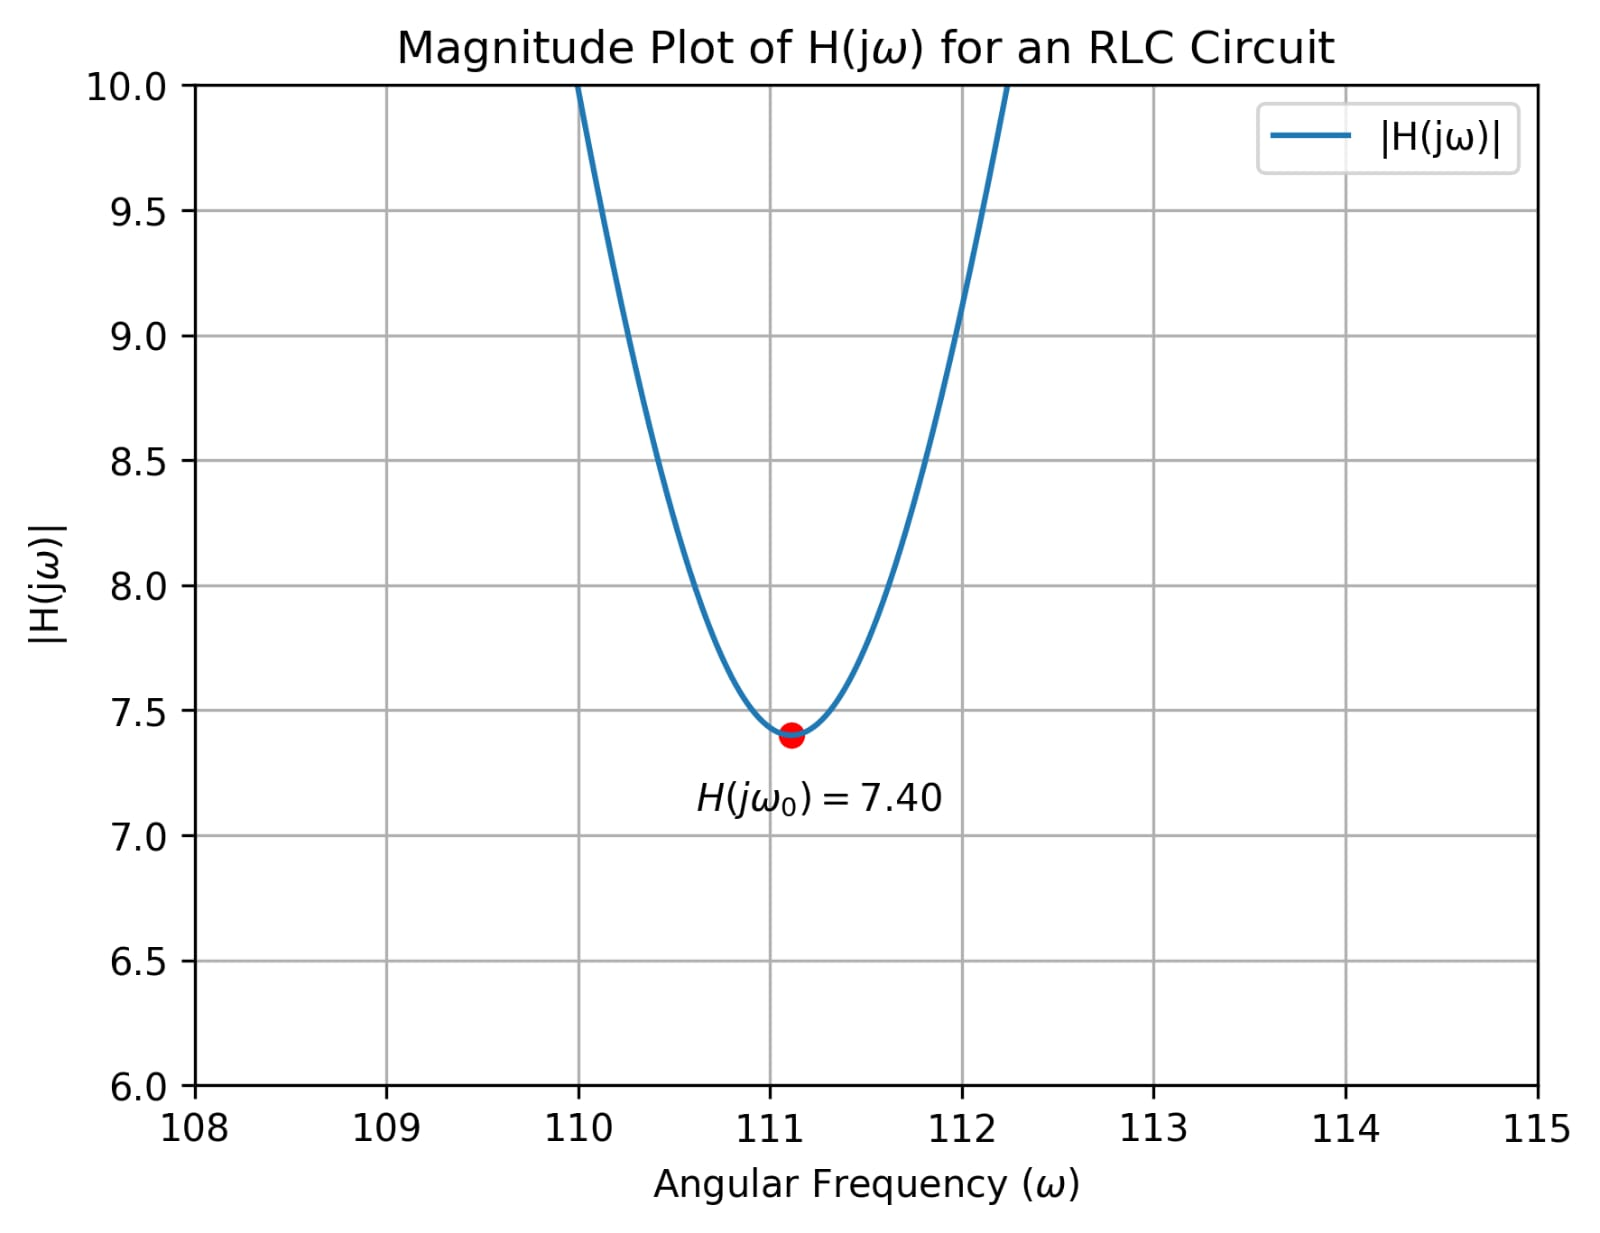
\includegraphics[width = \columnwidth]{ncert-physics/12/7/21/h_plot.png}
    \caption{Impedance vs $\omega$ (using values in \tabref{tab:1})}
    \label{fig:h_plot}
\end{figure}
\end{enumerate}


\pagebreak
\item A circuit containing a $80 mH$ inductor and a $60 \mu F$ capacitor in series is connected to a $230 V$, $50 Hz$ supply. A resistance of $15 \Omega $ is connected in series. Obtain the average power transferred to each element of the circuit, and the total power absorbed.\\
\solution
\pagebreak

\item A series LCR circuit with 
\(L = 0.12 \, \text{H}\),
\(C = 480 \times 10^{-9} \, \text{F}\), 
\(R=23 \, \Omega\)
is connected to a 230 V variable frequency supply.
(a) What is the source frequency for which current amplitude is maximum? Obtain this maximum value.

(b) What is the source frequency for which the average power absorbed by the circuit is maximum? Obtain the value of this maximum power.

(c) For which frequencies of the source is the power transferred to the circuit half the power at resonant frequency? What is the current amplitude at these frequencies?

(d) What is the Q-factor of the given circuit?
\end{enumerate}

\chapter{ Z-transform}
\begin{enumerate}[label=\thesection.\arabic*,ref=\thesection.\theenumi]
\item The $4^{th}$ term of a G.P. is square of its second term, and the first term is -3. Determine its $7^{th}$ term.\\  

\solution 

\iffalse
\documentclass[journal,12pt,twocolumn]{IEEEtran}
\usepackage{amsmath,amssymb,amsfonts,amsthm}
\usepackage{txfonts}
\usepackage{tkz-euclide}
\usepackage{listings}
\usepackage{gvv}
\usepackage[latin1]{inputenc}
\usepackage{array}
\usepackage{pgf}
\usepackage{lmodern}

\begin{document}
\bibliographystyle{IEEEtran}

\title{DISCRETE 11.9.3 Q-4}
\author{EE23BTECH11066 - Yakkala Amarnath Karthik
}
\maketitle

\bibliographystyle{IEEEtran}
\textbf{Question:} \\ \\The $4^{th}$ term of a G.P. is square of its second term, and the first term is -3. Determine its $7^{th}$ term.\\ \\
\textbf{Solution:}
\fi
\begin{table}[h!]
  \centering
    \begin{tabular}{|c|c|c|}
    \hline
    \textbf{Variable} & \textbf{Description} & \textbf{value}\\
    \hline
    $x(0)$ & first term of G.P. & -3 \\
    \hline
    $r$ & Common ratio of G.P. & ? \\
    \hline
    $x(n)$ & general term of the G.P. & $x\brak0r^{n}$ \\
    \hline
    $x\brak3$ & fourth term & $\sbrak{x\brak1}^2$\\
    \hline
    $u\brak{n}$ & unit step function & - \\
    \hline
  \end{tabular}

  \caption{A Table with input parameters}
  \label{tab:11.9.3.4.1}
\end{table}
from \tabref{tab:11.9.3.4.1}
\begin{align}
 x\brak0r^{3}&=\brak{x\brak0r^{1}}^2\\
 &=x\brak0^2r^2\\
\implies r&=x\brak0\\
&=-3
\end{align}
general term
\begin{align}
x\brak{n}&=x\brak0r^nu\brak{n}\\
&=\brak{-3}^{n+1}u\brak{n}
\end{align}
The $7^{th}$ term of the sequence will be:
\begin{align}
x\brak6 & =\brak{-3}\brak{-3}^{6}\\
& =-2187
\end{align}
Z transform of the given G.P is:
\begin{align}
X\brak{z}=\frac{x\brak0}{1-rz^{-1}}= \frac{-3}{1+3z^{-1}}.\hspace{0.5cm} |z|>3
\end{align}
\bigskip
\begin{figure}[ht]
        \centering
        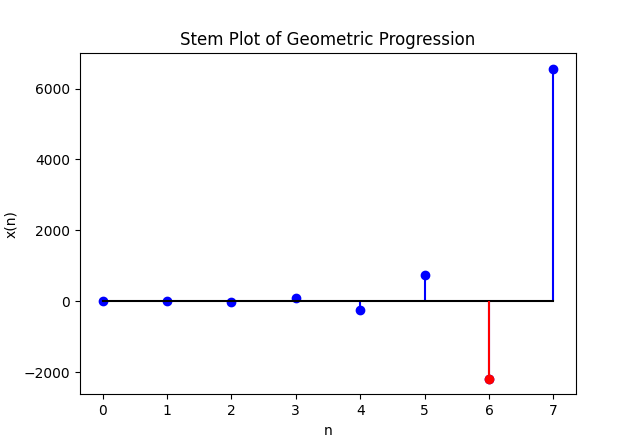
\includegraphics[width=0.45\textwidth]{ncert-maths/11/9/3/4/figs/stemplotfinal.jpeg}
        \caption{Graph showing first 8 terms of the GP}
    \end{figure} \\
%\end{document}

\pagebreak

\item Show that
\begin{equation}
    \frac{1\times2^2 + 2\times3^2 + \dots + n\times\brak{n+1}^2}{1^2\times2 + 2^2\times3 +\dots + n^2\times\brak{n+1}}  = \frac{3n+5}{3n+1}\notag
\end{equation}

\solution 

\iffalse
\let\negmedspace\undefined
\let\negthickspace\undefined
\documentclass[journal,12pt,twocolumn]{IEEEtran}
\usepackage{cite}
\usepackage{amsmath,enumitem,amssymb,amsfonts,amsthm}
\usepackage{algorithmic}
\usepackage{graphicx}
\usepackage{float}
\usepackage{textcomp}
\usepackage{xcolor}
\usepackage{caption}
\usepackage{txfonts}
\usepackage{listings}
\usepackage{enumitem}
\usepackage{mathtools}
\usepackage{gensymb}
\usepackage{comment}
\usepackage[breaklinks=true]{hyperref} 
\usepackage{tkz-euclide} 
\usepackage{listings}
\usepackage{tabularx}
\usepackage{gvv}                                        
\def\inputGnumericTable{}                                 
\usepackage[latin1]{inputenc}                              
\usepackage{color}                                            
\usepackage{array}                                            
\usepackage{longtable}                                       
\usepackage{calc}                                             
\usepackage{multirow}                                         
\usepackage{hhline}                                           
\usepackage{ifthen}                                        
\usepackage{lscape}
\newtheorem{theorem}{Theorem}[section]
\newtheorem{problem}{Problem}
\newtheorem{proposition}{Proposition}[section]
\newtheorem{lemma}{Lemma}[section]
\newtheorem{corollary}[theorem]{Corollary}
\newtheorem{example}{Example}[section]
\newtheorem{definition}[problem]{Definition}
\newcommand{\BEQA}{\begin{eqnarray}}
\newcommand{\EEQA}{\end{eqnarray}}
\newcommand{\define}{\stackrel{\triangle}{=}}
\theoremstyle{remark}
\newtheorem{rem}{Remark}
\begin{document}
\bibliographystyle{IEEEtran}
\vspace{3cm}
\title{NCERT 11.9.5 26Q}
\author{EE23BTECH11015 - DHANUSH V NAYAK$^{*}$% <-this % stops a space
}
\maketitle
\newpage
\bigskip
\renewcommand{\thefigure}{\arabic{figure}}
\renewcommand{\thetable}{\theenumi}
\bibliographystyle{IEEEtran}
\textbf{\underline{RESULTS AND DERIVATIONS}}

\newpage
\textbf{Question:} Show that
\begin{equation}
    \frac{1\times2^2 + 2\times3^2 + \dots + n\times\brak{n+1}^2}{1^2\times2 + 2^2\times3 +\dots + n^2\times\brak{n+1}}  = \frac{3n+5}{3n+1}\notag
\end{equation}
\textbf{Solution:}
\fi 

\begin{table}[h]
    \centering
    \renewcommand\thetable{1}
    \setlength{\extrarowheight}{9pt}
    \resizebox{0.54\textwidth}{!}{
    \begin{tabular}{|c|c|c|}
    \hline
    \textbf{Parameter} & \textbf{Description} & \textbf{Value} \\ \hline
    $n$ & Integer &.... -2,-1,0,1, 2, ... \\ \hline
    $x_1(n)$ & General term of Numerator & $\vphantom{\brak{n^{3}}} \brak{n^{3} + 5n^{2} + 8n + 4} \cdot u\brak{n}$ \\ \hline
    $x_2(n)$ & General Term of Denominator  & $\vphantom{\brak{n^{3}}} \brak{n^{3}+4n^{2}+5n+2}\cdot u\brak{n}$ \\ \hline
    $y_1\brak{n}$ & Sum of terms of numerator & $?$ \\ \hline
    $y_2\brak{n}$ & Sum of terms of denominator & $? $ \\ \hline
    $U(z)$ & z-transform of $u(n)$ & $\frac{1}{1 - z^{-1}\vphantom {\brak{0.3pt}}},\cbrak{z\in\mathbb{C} : \lvert z \rvert > 1}$ \\ \hline 
    ROC & Region of convergence & $\left\{ z : \left|\sum_{n=-\infty}^{\infty} x(n)z^{-n}\right| < \infty \vphantom {\brak{{0.3pt}}}\right\}$ \\ \hline 
    \end{tabular}}
    \caption{Parameter Table}
    \label{tab:11.9.5.26.1}
    \end{table}
    
    
    
    
\begin{enumerate}[label=\arabic*.]
\item \underline {Analysis of Numerator:}\\
\begin{align}
 X_1\brak{z} &= \sum_{n=-\infty}^\infty x_1\brak{n}  z^{-n}\\
             &= \sum_{n=-\infty}^\infty \brak{n^{3} + 5n^{2} + 8n + 4} u\brak{n} z^{-n}
\end{align}
Using results of equations \eqref{eq:11.9.5.26.2} to \eqref{eq:11.9.5.26.5} we get:
\begin{align}
 \therefore   X_1\brak{z}&= \frac{4+2z^{-1}}{\brak{1-z^{-1}}^4} ,   \abs{z} >1 
\end{align}
From \eqref{eq:conv-sum}
\begin{align}
y_1\brak{n} &= x_1\brak{n}\ast u\brak{n}\\
    Y_1\brak{z} &= X_1\brak{z} U\brak{z} \\
 &= \frac{4+2z^{-1}}{\brak{1-z^{-1}}^5} , \abs{z}> 1 
\end{align}
Using partial fractions:
\begin{align}
    Y_1(z) &= \frac{22z^{-1}}{\brak{1-z^{-1}}} + \frac{48z^{-2}}{\brak{1-z^{-1}}^2} + \frac{52z^{-3}}{\brak{1-z^{-3}}^3} , \label{eq:11.9.5.26.6}\\
    &+ \frac{28z^{-4}}{\brak{1-z^{-1}}^4}+\frac{6z^{-5}}{\brak{1-z^{-1}}^5}+4 , \abs{z}>1 \notag 
\end{align}
Substituting results of equation \eqref{eq:11.9.5.26.9} to \eqref{eq:11.9.5.26.12} in equation \eqref{eq:11.9.5.26.6}:
\begin{align}
    y_1\brak{n} &= \frac{3n^4 + 26n^3 + 81n^2 + 106n + 48}{12}u\brak{n}\\
    &= \frac{\brak{3n+8}\brak{n+1}\brak{n+2}\brak{n+3}}{12}u\brak{n}
\end{align}
\item \underline{Analysis of Denominator:}
\begin{align}
    X_2\brak{z} &= \sum_{n=-\infty}^\infty x_2\brak{n} z^{-n}\\
                &= \sum_{n=-\infty}^\infty \brak{n^{3}+4n^{2}+5n+2} u\brak{n} z^{-n}
\end{align}
\text{Using results of equation \eqref{eq:11.9.5.26.2} to \eqref{eq:11.9.5.26.5} we get:}
\begin{align}
   \therefore  X_2\brak{z} &= \frac{2+4z^{-1}}{\brak{1-z^{-1}}^4},   \abs{z} >1   
\end{align}
From \eqref{eq:conv-sum}
\begin{align}
    y_2\brak{n} &= x_2\brak{n}\ast u\brak{n}\\
    Y_2\brak{z} &= X_2\brak{z} U\brak{z} \\
 &=\frac{2+4z^{-1}}{\brak{1-z^{-1}}^5} ,   \abs{z} >1 
\end{align}
Using partial fractions:
\begin{align}
    Y_2\brak{z} &= \frac{14z^{-1}}{\brak{1-z^{-1}}} + \frac{36z^{-2}}{\brak{1-z^{-1}}^2} + \frac{44z^{-3}}{\brak{1-z^{-3}}^3} \label{eq:11.9.5.26.13}\\
    &+ \frac{26z^{-4}}{\brak{1-z^{-1}}^4}+\frac{6z^{-5}}{\brak{1-z^{-1}}^5}+2 , \abs{z}>1\notag 
\end{align}
Substituting results of equation \eqref{eq:11.9.5.26.9} to \eqref{eq:11.9.5.26.12} in equation \eqref{eq:11.9.5.26.13}:
\begin{align}
    y_2\brak{n} &=  \frac{3n^4 + 22n^3 + 57n^2 + 62n + 24}{12}u\brak{n}\\
                &= \frac{\brak{3n+4}\brak{n+1}\brak{n+2}\brak{n+3}}{12}u\brak{n}
\end{align}
As the sequence start from $n=0$ , in RHS of question $n$ should be replaced by $n+1$:
\begin{align}
    \frac{y_1\brak{n}}{y_2\brak{n}} = \frac{3n+8}{3n+4}
\end{align}
Hence Prooved.
\end{enumerate}
\begin{figure}[htbp]
    \centering
    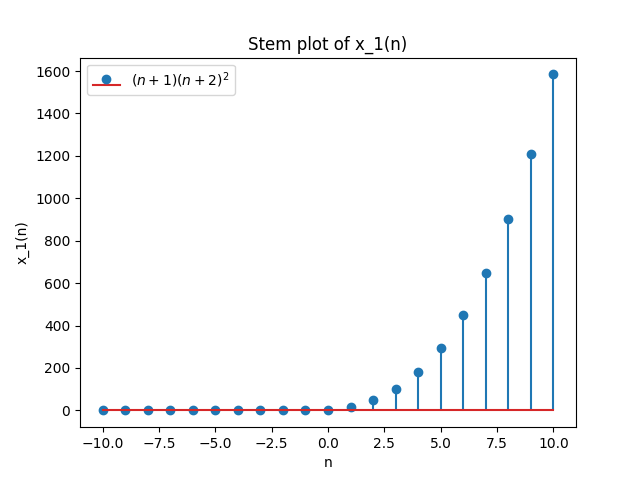
\includegraphics[width=1\columnwidth]{ncert-maths/11/9/5/26/figs/x1_plot.png}
    \caption{Stem Plot of $x_1\brak{n}$}
    \label{fig:x1}
\end{figure}
\begin{figure}[htbp]
    \centering
    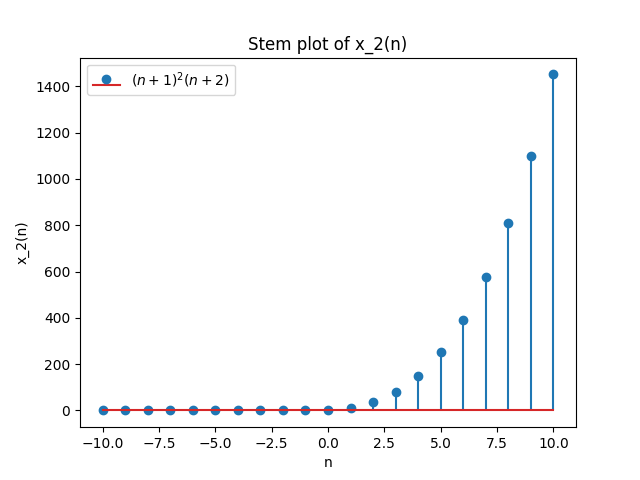
\includegraphics[width=1\columnwidth]{ncert-maths/11/9/5/26/figs/x2_plot.png}
    \caption{Stem Plot of $x_2\brak{n}$}
    \label{fig:x2}
\end{figure}
\begin{figure}[htbp]
    \centering
    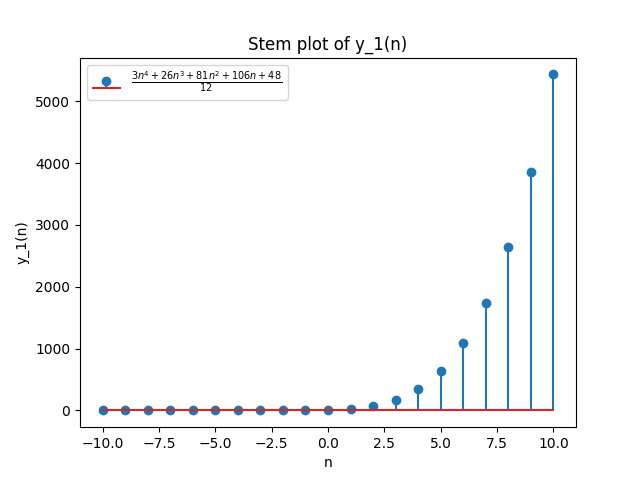
\includegraphics[width=1\columnwidth]{ncert-maths/11/9/5/26/figs/y1_plot.png}
    \caption{Stem Plot of $y_1\brak{n}$}
    \label{fig:y1}
\end{figure}
\begin{figure}[h]
    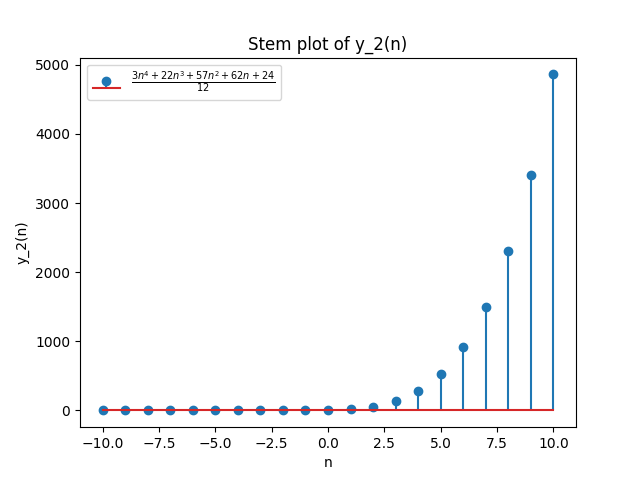
\includegraphics[width=1\columnwidth]{ncert-maths/11/9/5/26/figs/y2_plot.png}
    \caption{Stem Plot of $y_2\brak{n}$}
    \label{fig:y2}
\end{figure}
%\end{document}

\pagebreak

\item Write the five terms at n = 1, 2, 3, 4, 5 of the sequence and obtain the Z-transform of the series
\begin{align}
    x \brak{n} &=  -1, & n = 0 \\
    &=   \frac{x \brak{n-1}}{n}, & n > 0\\
    &=   0, & n < 0 
\end{align}

\solution

\iffalse
\let\negmedspace\undefined
\let\negthickspace\undefined
\documentclass[journal,12pt,twocolumn]{IEEEtran}
\usepackage{cite}
\usepackage{amsmath,amssymb,amsfonts}
\usepackage{graphicx}
\usepackage{textcomp}
\usepackage{xcolor}
\usepackage{txfonts}
\usepackage{listings}
\usepackage{enumitem}
\usepackage{mathtools}
\usepackage{gensymb}
\usepackage{comment}
\usepackage[breaklinks=true]{hyperref}
\usepackage{tkz-euclide} 
\usepackage{listings}
\usepackage{gvv}                                        
\def\inputGnumericTable{}                                 
\usepackage[latin1]{inputenc}                                
\usepackage{color}                                            
\usepackage{array}                                            
\usepackage{longtable}                                       
\usepackage{calc}                                             
\usepackage{multirow}                                         
\usepackage{hhline}                                           
\usepackage{ifthen}                                           
\usepackage{lscape}
\usepackage[export]{adjustbox}

\newtheorem{theorem}{Theorem}[section]
\newtheorem{problem}{Problem}
\newtheorem{proposition}{Proposition}[section]
\newtheorem{lemma}{Lemma}[section]
\newtheorem{corollary}[theorem]{Corollary}
\newtheorem{example}{Example}[section]
\newtheorem{definition}[problem]{Definition}
\newcommand{\BEQA}{\begin{eqnarray}}
\newcommand{\EEQA}{\end{eqnarray}}
\newcommand{\define}{\stackrel{\triangle}{=}}
\newtheorem{rem}{Remark}

\begin{document}
\parindent 0px
\bibliographystyle{IEEEtran}

\vspace{3cm}

\title{}
\author{EE23BTECH11217 - Prajwal M$^{*}$
}
\maketitle
\newpage
\bigskip

 \renewcommand{\thefigure}{\theenumi}
 \renewcommand{\thetable}{\theenumi}


\section*{Exercise 9.1}

\noindent \textbf{12} \hspace{2pt}Write the five terms at n = 1, 2, 3, 4, 5 of the sequence and obtain the Z-transform of the series
\begin{align}
    x \brak{n} &=  -1, & n = 0 \\
    &=   \frac{x \brak{n-1}}{n}, & n > 0\\
    &=   0, & n < 0 
\end{align}

\noindent Solution:
\fi
\noindent
\begin{align}
	x \brak{1} & = \frac{x \brak{0}}{1} = -1 \\
x \brak{2} & = \frac{x \brak{1}}{2} = -\frac{1}{2} \\
	x \brak{3} & = \frac{x \brak{2}}{3} = -\frac{1}{\brak{2} \brak{3}} = -\frac{1}{6}\\
	x \brak{4} & = \frac{x \brak{3}}{4} = -\frac{1}{\brak{2}   \brak{3} \brak{4}} = -\frac{1}{24}\\
	x \brak{5} & = \frac{x \brak{4}}{5} = -\frac{1}{\brak{2} \brak{3} \brak{4} \brak{5}} = -\frac{1}{120} \\
    x \brak{n} & = \frac{-1}{n!}  \brak{u \brak{n}} \label{x(n)}
\end{align}
\begin{align}
	x \brak{n} & \system{Z} X \brak{z} 
\end{align}

\begin{figure}[h]
   \centering
   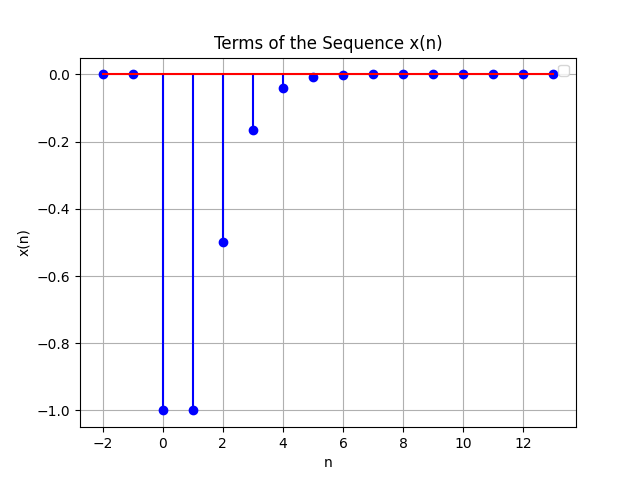
\includegraphics[width=1\columnwidth]{ncert-maths/11/9/1/12/figs/plot.png}
   \caption{Plot of x(n) vs n}
   \label{fig: 9.1.12.1}
\end{figure}

\begin{align}
    X \brak{z} & = \sum_{n=-\infty}^{\infty} x \brak{n}   z^{-n} \\
    \notag \text{using \eqref{x(n)}, } \\
    & = \sum_{n=-\infty}^{\infty} \frac{-1}{n!}  u \brak{n}   z^{-n} \\
    & = \sum_{n=0}^{\infty} \frac{-1}{n!}   z^{-n} \\
    & = - e^{z^{-1}} &  \cbrak{z\in\mathbb{C} : z \neq 0} 
\end{align}

\begin{table}[h]
    \centering
      \begin{tabular}{|c|c|c|}
    \hline
    	\textbf{Symbol} & \textbf{Value} & \textbf{Description} \\
    \hline
	  $x(n)$ & $\frac{-1}{n!}$ & general term of the series \\
    \hline
	  $X(z)$ & $- e^{z^{-1}}$ &Z-transform of x(n) \\
    \hline 
	  $u(n)$ & &unit step function \\
    \hline
  \end{tabular}

    \caption{Parameters}
    \label{tab: 9.1.12.1}
\end{table}


%\end{document}

\pagebreak


\item Subba Rao started work in 1995 at an annual salary of Rs. 5000 and received an increment of Rs. 200 each year. In which year did his income reach Rs. 7000?

\solution

\iffalse
\let\negmedspace\undefined
\let\negthickspace\undefined
\documentclass[journal,12pt,twocolumn]{IEEEtran}
\usepackage{cite}
\usepackage{amsmath,amssymb,amsfonts,amsthm}
\usepackage{algorithmic}
\usepackage{graphicx}
\usepackage{textcomp}
\usepackage{xcolor}
\usepackage{txfonts}
\usepackage{listings}
\usepackage{enumitem}
\usepackage{mathtools}
\usepackage{gensymb}
\usepackage{comment}
\usepackage[breaklinks=true]{hyperref}
\usepackage{tkz-euclide}
\usepackage{listings}
\usepackage{gvv}
\def\inputGnumericTable{}
\usepackage[latin1]{inputenc}
\usepackage{color}
\usepackage{array}
\usepackage{longtable}
\usepackage{calc}
\usepackage{multirow}
\usepackage{hhline}
\usepackage{ifthen}
\usepackage{lscape}

\newtheorem{theorem}{Theorem}[section]
\newtheorem{problem}{Problem}
\newtheorem{proposition}{Proposition}[section]
\newtheorem{lemma}{Lemma}[section]
\newtheorem{corollary}[theorem]{Corollary}
\newtheorem{example}{Example}[section]
\newtheorem{definition}[problem]{Definition}
\newcommand{\BEQA}{\begin{eqnarray}}
\newcommand{\EEQA}{\end{eqnarray}}
\newcommand{\define}{\stackrel{\triangle}{=}}
\theoremstyle{remark}
\newtheorem{rem}{Remark}
\begin{document}

\bibliographystyle{IEEEtran}
\vspace{3cm}

\title{NCERT Discrete - 10.5.2.19}
\author{EE23BTECH11007 - Aneesh Kadiyala$^{*}$% <-this % stops a space
}
\maketitle
\newpage
\bigskip

\renewcommand{\thefigure}{\theenumi}
\renewcommand{\thetable}{\theenumi}
\vspace{3cm}
\textbf{Question 10.5.2.19:} Subba Rao started work in 1995 at an annual salary of Rs. 5000 and received an increment of Rs. 200 each year. In which year did his income reach Rs. 7000?

\solution
\fi
\begin{table}[h!]
    \centering
    \begin{tabular}{ | c | c | c | }
        \hline
        Parameter & Value & Description \\
        \hline
        $x(0)$ & 5000 & Initial Income \\
        \hline
        $d$ & 200 & Annual Increment (Common Difference) \\
        \hline
        $x(n)$ & $(x(0) + nd)u(n)$ & $n^{th}$ term of the AP \\
        \hline
    \end{tabular}
    \caption{Input Parameters}
    \label{tab:math_10_5_2_19}
\end{table}
From the values given in \tabref{tab:math_10_5_2_19}:
\begin{align}
7000 &= 5000 + 200n \\
\implies 2000 &= 200n \\
\therefore n &= 10
\end{align}
\begin{figure}[h!]
    \centering
    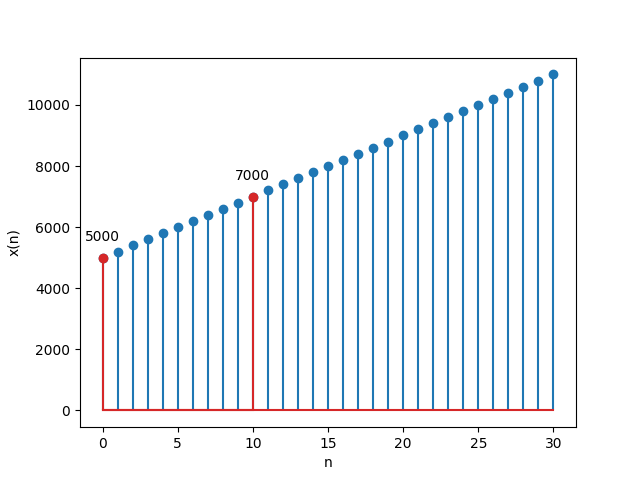
\includegraphics[width=\columnwidth]{ncert-maths/10/5/2/19/figs/10_5_2_19.png}
    \caption{Plot of $x(n)$ vs $n$. See \tabref{tab:math_10_5_2_19} for details.}
    \label{fig:math_10_5_2_19}
\end{figure}
Let Z-transform of $x(n)$ be $X(z)$.
\begin{align}
X(z) &= \frac{x(0)}{1 - z^{-1}} + \frac{dz^{-1}}{(1 - z^{-1})^2} \quad |z| > 1
\end{align}
Using the values from \tabref{tab:math_10_5_2_19}:
\begin{align}
X(z) &= \frac{5000}{1 - z^{-1}} + \frac{200z^{-1}}{(1 - z^{-1})^2} \quad |z| > 1
\end{align}
%\end{document}


\item Consider the sequence whose $n^\text{th}$ term is given by \(2^n\). Find the first 6 terms of this sequence.

\solution

%\iffalse
\let\negmedspace\undefined
\let\negthickspace\undefined
\documentclass[journal,12pt,onecolumn]{IEEEtran}
\usepackage{cite}
\usepackage{amsmath,amssymb,amsfonts,amsthm}
%\usepackage{algorithmic}
\usepackage{graphicx}
\usepackage{textcomp}
\usepackage{array}
\usepackage{xcolor}
\usepackage{txfonts}
\usepackage{listings}
\usepackage{enumitem}
\usepackage{mathtools}
\usepackage{gensymb}
\usepackage[breaklinks=true]{hyperref}
\usepackage{tkz-euclide} % loads  TikZ and tkz-base
\usepackage{listings}
\usepackage{float}



\newtheorem{theorem}{Theorem}[section]
\newtheorem{problem}{Problem}
\newtheorem{proposition}{Proposition}[section]
\newtheorem{lemma}{Lemma}[section]
\newtheorem{corollary}[theorem]{Corollary}
\newtheorem{example}{Example}[section]
\newtheorem{definition}[problem]{Definition}
%\newtheorem{thm}{Theorem}[section] 
%\newtheorem{defn}[thm]{Definition}
%\newtheorem{algorithm}{Algorithm}[section]
%\newtheorem{cor}{Corollary}
\newcommand{\BEQA}{\begin{eqnarray}}
\newcommand{\EEQA}{\end{eqnarray}}
\newcommand{\define}{\stackrel{\triangle}{=}}
\theoremstyle{remark}
\newtheorem{rem}{Remark}
%\bibliographystyle{ieeetr}
\begin{document}
%
\providecommand{\pr}[1]{\ensuremath{\Pr\left(#1\right)}}
\providecommand{\prt}[2]{\ensuremath{p_{#1}^{\left(#2\right)} }}        % own macro for this question
\providecommand{\qfunc}[1]{\ensuremath{Q\left(#1\right)}}
\providecommand{\sbrak}[1]{\ensuremath{{}\left[#1\right]}}
\providecommand{\lsbrak}[1]{\ensuremath{{}\left[#1\right.}}
\providecommand{\rsbrak}[1]{\ensuremath{{}\left.#1\right]}}
\providecommand{\brak}[1]{\ensuremath{\left(#1\right)}}
\providecommand{\lbrak}[1]{\ensuremath{\left(#1\right.}}
\providecommand{\rbrak}[1]{\ensuremath{\left.#1\right)}}
\providecommand{\cbrak}[1]{\ensuremath{\left\{#1\right\}}}
\providecommand{\lcbrak}[1]{\ensuremath{\left\{#1\right.}}
\providecommand{\rcbrak}[1]{\ensuremath{\left.#1\right\}}}
\newcommand{\sgn}{\mathop{\mathrm{sgn}}}
\providecommand{\abs}[1]{\left\vert#1\right\vert}
\providecommand{\res}[1]{\Res\displaylimits_{#1}} 
\providecommand{\norm}[1]{\left\lVert#1\right\rVert}
%\providecommand{\norm}[1]{\lVert#1\rVert}
\providecommand{\mtx}[1]{\mathbf{#1}}
\providecommand{\mean}[1]{E\left[ #1 \right]}
\providecommand{\cond}[2]{#1\middle|#2}
\providecommand{\fourier}{\overset{\mathcal{F}}{ \rightleftharpoons}}
\newenvironment{amatrix}[1]{%
  \left(\begin{array}{@{}*{#1}{c}|c@{}}
}{%
  \end{array}\right)
}
%\providecommand{\hilbert}{\overset{\mathcal{H}}{ \rightleftharpoons}}
%\providecommand{\system}{\overset{\mathcal{H}}{ \longleftrightarrow}}
	%\newcommand{\solution}[2]{\textbf{Solution:}{#1}}
\newcommand{\solution}{\noindent \textbf{Solution: }}
\newcommand{\cosec}{\,\text{cosec}\,}
\providecommand{\dec}[2]{\ensuremath{\overset{#1}{\underset{#2}{\gtrless}}}}
\newcommand{\myvec}[1]{\ensuremath{\begin{pmatrix}#1\end{pmatrix}}}
\newcommand{\mydet}[1]{\ensuremath{\begin{vmatrix}#1\end{vmatrix}}}
\newcommand{\myaugvec}[2]{\ensuremath{\begin{amatrix}{#1}#2\end{amatrix}}}
\providecommand{\rank}{\text{rank}}
\providecommand{\pr}[1]{\ensuremath{\Pr\left(#1\right)}}
\providecommand{\qfunc}[1]{\ensuremath{Q\left(#1\right)}}
	\newcommand*{\permcomb}[4][0mu]{{{}^{#3}\mkern#1#2_{#4}}}
\newcommand*{\perm}[1][-3mu]{\permcomb[#1]{P}}
\newcommand*{\comb}[1][-1mu]{\permcomb[#1]{C}}
\providecommand{\qfunc}[1]{\ensuremath{Q\left(#1\right)}}
\providecommand{\gauss}[2]{\mathcal{N}\ensuremath{\left(#1,#2\right)}}
\providecommand{\diff}[2]{\ensuremath{\frac{d{#1}}{d{#2}}}}
\providecommand{\myceil}[1]{\left \lceil #1 \right \rceil }
\newcommand\figref{Fig.~\ref}
\newcommand\tabref{Table~\ref}
\newcommand{\sinc}{\,\text{sinc}\,}
\newcommand{\rect}{\,\text{rect}\,}
%%
%	%\newcommand{\solution}[2]{\textbf{Solution:}{#1}}
%\newcommand{\solution}{\noindent \textbf{Solution: }}
%\newcommand{\cosec}{\,\text{cosec}\,}
%\numberwithin{equation}{section}
%\numberwithin{equation}{subsection}
%\numberwithin{problem}{section}
%\numberwithin{definition}{section}
%\makeatletter
%\@addtoreset{figure}{problem}
%\makeatother

%\let\StandardTheFigure\thefigure
\let\vec\mathbf

\bibliographystyle{IEEEtran}





\bigskip

%\renewcommand{\thefigure}{\theenumi}
%\renewcommand{\thetable}{\theenumi}
%\renewcommand{\theequation}{\theenumi}

Q: Consider the sequence whose $n^\text{th}$ term is given by \(2^n\). Find the first 6 terms of this sequence.

\solution

\begin{table}[!ht]
    \centering
        \begin{table}[ht]
    \centering
    \begin{tabular}{|c|c|c|}
        \hline
        Parameter & Value & Description \\
        \hline
        $x(0)$ & 5 & First term of AP \\
        $d$ & 1.75 & Common difference of AP \\
        $x(n)$ & 20.75 & $n^{th}$ term of AP \\
        \hline
    \end{tabular}
    \vspace{2mm}
    \caption{Parameter List}
    \label{tab:simple.10.5.2.20}
\end{table}

    \caption{input parameters}
    \label{tab:11_9_1_3}
\end{table}
%\fi
\begin{align}
X(Z) &= \frac {1}{1 - 2  z^{-1} } \quad \abs{z}>\abs{2}
\end{align}

\begin{figure}[H]
    \centering
    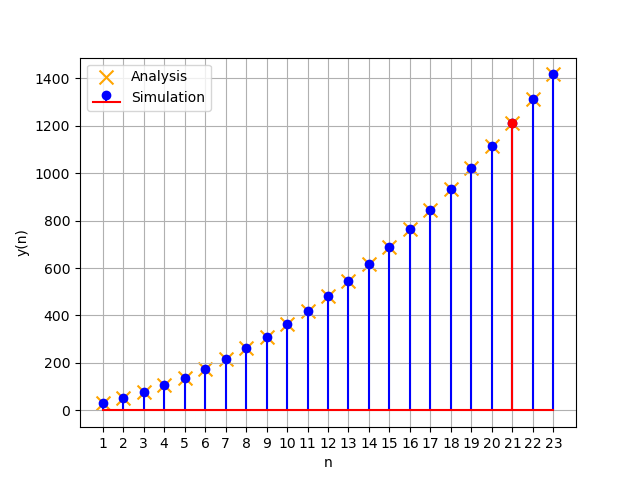
\includegraphics{figs/fig1.png}
    \caption{Six terms of given sequence}
    \label{fig:11_9_1_3 }
\end{figure}

\end{document}


\item If the sum of first 7 terms of an AP is 49 and that of 17 terms is 289, find the sum of first n terms.

\solution

\iffalse
\let\negmedspace\undefined
\let\negthickspace\undefined
\documentclass[journal,12pt,twocolumn]{IEEEtran}
\usepackage{cite}
\usepackage{amsmath,amssymb,amsfonts,amsthm}
\usepackage{algorithmic}
\usepackage{graphicx}
\usepackage{textcomp}
\usepackage{xcolor}
\usepackage{txfonts}
\usepackage{listings}
\usepackage{enumitem}
\usepackage{mathtools}
\usepackage{gensymb}
\usepackage{comment}
\usepackage[breaklinks=true]{hyperref}
\usepackage{tkz-euclide} 
\usepackage{listings}
\usepackage{gvv}                                        
\def\inputGnumericTable{}                                 
\usepackage[latin1]{inputenc}                                
\usepackage{color}                                            
\usepackage{array}                                            
\usepackage{longtable}                                       
\usepackage{calc}                                             
\usepackage{multirow}                                         
\usepackage{hhline}                                           
\usepackage{ifthen}                                           
\usepackage{lscape}
\newtheorem{theorem}{Theorem}[section]
\newtheorem{problem}{Problem}
\newtheorem{proposition}{Proposition}[section]
\newtheorem{lemma}{Lemma}[section]
\newtheorem{corollary}[theorem]{Corollary}
\newtheorem{example}{Example}[section]
\newtheorem{definition}[problem]{Definition}
\newcommand{\BEQA}{\begin{eqnarray}}
\newcommand{\EEQA}{\end{eqnarray}}
\newcommand{\define}{\stackrel{\triangle}{=}}
\theoremstyle{remark}
\newtheorem{rem}{Remark}
\begin{document}

\bibliographystyle{IEEEtran}
\vspace{3cm}

\title{10.5.3.9}
\author{EE23BTECH11063 - Vemula Siddhartha
}
\maketitle
\newpage
\bigskip

\renewcommand{\thefigure}{\theenumi}
\renewcommand{\thetable}{\theenumi}
\textbf{Question}:\\
If the sum of first 7 terms of an AP is 49 and that of 17 terms is 289, find the sum of
first n terms.
\\
\textbf{Solution: }
\fi
\begin{table}[h!]    
  \centering
  \begin{tabular}[12pt]{ |c| c|}
    \hline
    \textbf{Variable} & \textbf{Description}\\ 
    \hline
    $x\brak{0}$ & First term of the AP \\
    \hline 
    $d$ & Common difference of the AP\\
    \hline
    $y\brak{n}$ & Sum of $n+1$ terms of the AP\\
    \hline
    $x\brak{n}$ & General term\\
    \hline   
    \end{tabular}
  \caption{Variables Used}
  \label{tab10.5.3.9.1}
\end{table}
\begin{align}
y\brak{n}&=\frac{n+1}{2}\,\brak{2x\brak{0}+nd}\,u\brak{n}\label{eq10.5.3.9.1}\\
y\brak{6}&=49\\
y\brak{16}&=289
\end{align}
Then,
\begin{align}
x\brak{0}+3d&=7\label{eq10.5.3.9.2}\\
x\brak{0}+8d&=17 \label{eq10.5.3.9.3}
\end{align}
From  equations \ref{eq10.5.3.9.2} and \ref{eq10.5.3.9.3}, the augmented matrix is:
\begin{align}
 \myvec{
   1 & 3 & 7
   \\
   1 & 8 & 17
 }
 \xleftrightarrow[]{R_2 \leftarrow {R_2-R_1}}
 \myvec{
   1 & 3 & 7
   \\
   0 & 5 & 10
 }
 \\
 \xleftrightarrow[]{R_1 \leftarrow {R_1-\frac{3}{5}R_2}}
 \myvec{
   1 & 0 & 1
   \\
   0 & 5 & 10
 }
 \\
 \xleftrightarrow[]{R_2 \leftarrow \frac{R_2}{5}}
 \myvec{
   1 & 0 & 1
   \\
   0 & 1 & 2
 }
 \\
 \implies \myvec{
   x\brak{0}
   \\
   d
 }
 =
 \myvec{
   1
   \\
   2
 }
\end{align}
\begin{align}
    x\brak{n}&= \brak{1+2n}u\brak{n}\\
    X\brak{z}&=\frac{1}{1-z^{-1}}+\frac{2z^{-1}}{\brak{1-z^{-1}}^2}\;\;\cbrak{z\in\mathbb{C}: |z|>1}
\end{align}
\begin{align}
   y\brak{n}&=x\brak{n}*u\brak{n}\\
   Y\brak{z}&=X\brak{z}\,U\brak{z}\\
   \implies Y\brak{z}&=\brak{\frac{1}{1-z^{-1}}+\frac{2z^{-1}}{\brak{1-z^{-1}}^2}}\brak{\frac{1}{1-z^{-1}}}\\
   &=\frac{1}{\brak{1-z^{-1}}^2}+\frac{2z^{-1}}{\brak{1-z^{-1}}^3}\\
   \brak{n+1}u\brak{n}&\system{Z}\frac{1}{\brak{1-z^{-1}}^2}\cbrak{z\in\mathbb{C}: |z|>1}\\
   n\brak{\brak{n+1}u\brak{n}}&\system{Z}\frac{2z^{-1}}{\brak{1-z^{-1}}^3}\cbrak{z\in\mathbb{C}: |z|>1}
\end{align}
   From equations \eqref{eq:uzder-shift} and \eqref{eq:uzder-der}, taking the inverse Z Transform,
   \begin{align}
   y\brak{n}&=\brak{n+1}u\brak{n}+n\brak{\brak{n+1}u\brak{n}}\\
   \implies y\brak{n}&=\brak{n+1}^2\,u\brak{n}
\end{align}
\begin{figure}[h!]
   \centering
   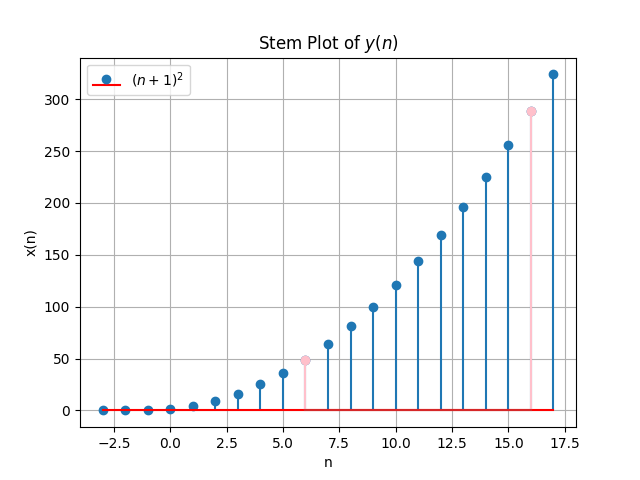
\includegraphics[width=1.1\linewidth]{ncert-maths/10/5/3/9/figs/Figure_1.png}
   \caption{Stem Plot of y\brak{n}}
   \label{stemplot}
\end{figure}  

\pagebreak

\item Write the first five terms of the sequence and obtain the corresponding series:\\
$a_1=a_2=2,$ $a_n=a_{n-1} -1,$ $n>2$\\
\solution
\iffalse
\let\negmedspace\undefined
\let\negthickspace\undefined
\documentclass[journal,12pt,twocolumn]{IEEEtran}
\usepackage{cite}
\usepackage{amsmath,amssymb,amsfonts,amsthm}
\usepackage{algorithmic}
\usepackage{graphicx}
\usepackage{textcomp}
\usepackage{xcolor}
\usepackage{txfonts}
\usepackage{listings}
\usepackage{enumitem}
\usepackage{mathtools}
\usepackage{float}
\usepackage{gensymb}
\usepackage{comment}
\usepackage[breaklinks=true]{hyperref}
\usepackage{tkz-euclide} 
\usepackage{listings}
\usepackage{gvv}                                        
\def\inputGnumericTable{}                                 
\usepackage[latin1]{inputenc}                                
\usepackage{color}                                            
\usepackage{array}                                            
\usepackage{longtable}                                       
\usepackage{calc}                                             
\usepackage{multirow}                                         
\usepackage{hhline}                                           
\usepackage{ifthen}                                           
\usepackage{lscape}
\usepackage{amsmath}
\newtheorem{theorem}{Theorem}[section]
\newtheorem{problem}{Problem}
\newtheorem{proposition}{Proposition}[section]
\newtheorem{lemma}{Lemma}[section]
\newtheorem{corollary}[theorem]{Corollary}
\newtheorem{example}{Example}[section]
\newtheorem{definition}[problem]{Definition}
\newcommand{\BEQA}{\begin{eqnarray}}
\newcommand{\EEQA}{\end{eqnarray}}
\newcommand{\define}{\stackrel{\triangle}{=}}
\theoremstyle{remark}
\newtheorem{rem}{Remark}
\begin{document}
\bibliographystyle{IEEEtran}
\title{NCERT 11.9.1.13Q}
\author{EE23BTECH11015 - DHANUSH V NAYAK$^{*}$% <-this % stops a space
}
\maketitle
\newpage
\bigskip
\renewcommand{\thefigure}{\arabic{figure}}
\renewcommand{\thetable}{\theenumi}
\textbf{Question:} Write the first five terms of each of the sequences in Exercises 11 to 13 and obtain the corresponding series:\\
$a_1=a_2=2,$\hspace{5pt} $a_n=a_{n-1} -1,$\hspace{5pt} $n>2$\\
\solution
\fi
\begin{table}[H]
    \centering
    \renewcommand\thetable{1}
    \setlength{\extrarowheight}{9pt}
    \resizebox{0.5\textwidth}{!}{
    \begin{tabular}{|c|c|c|}
    \hline
    \textbf{Parameter} & \textbf{Description} & \textbf{Value} \\ \hline
    $x\brak{0}$ & First term &2 \\ \hline
    $x\brak{1}$ & Second term &2 \\ \hline
    ROC & Region of convergence & $\left\{ z : \left|\sum_{n=-\infty}^{\infty} x(n)z^{-n}\right| < \infty \vphantom {\brak{{0.3pt}}}\right\}$ \\ \hline 
    $x(n)$ & General term & $x(n) = 
    \begin{cases}
        ? & ; n \geq 0 \\
        0 & ; n < 0 \\
    \end{cases}$ \\ \hline
    \end{tabular}}
    \caption{Parameter Table}
    \label{tab:11.9.1.13}
    \end{table}
\begin{align}
    x\brak{n} - x\brak{n-1} &= 2u\brak{n}-2u\brak{n-1}-u\brak{n-2}\label{eq:11.9.1.13.1}\\
X\brak{z}- z^{-1}X\brak{z} &= \frac{2}{\brak{1-z^{-1}}} - \frac{z^{-2}}{\brak{1-z^{-1}}}- \frac{2z^{-1}}{\brak{1-z^{-1}}}\\
    X\brak{z} &= \frac{2-2z^{-1}-z^{-2}}{\brak{1-z^{-1}}^2}  ,   \abs{z} >1
\end{align}
Using partial fractions
\begin{align}
    X\brak{z} &= \frac{2z^{-1}}{\brak{1-z^{-1}}} - \frac{z^{-2}}{\brak{1-z^{-1}}^2} + 2\label{eq:11.9.1.13.5}
\end{align}
Taking inverse $Z$-transform by result of equation \eqref{eq:11.9.5.26.9} in equation \eqref{eq:11.9.1.13.5}:
\begin{align}
    x\brak{n} &= 2u\brak{n}+\brak{1-n}u\brak{n-1}\label{eq:11.9.1.13.6}
\end{align}
\begin{figure}[H]
    \centering
    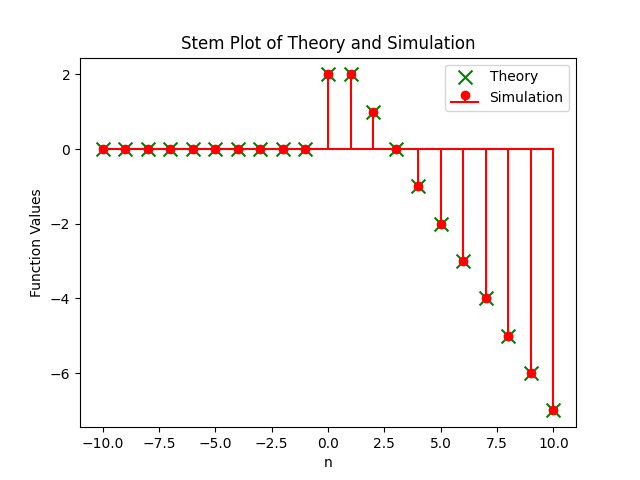
\includegraphics[width=1\columnwidth]{ncert-maths/11/9/1/13/figs/Theory_vs_Simulation.png}
    \caption{Comparison of Theory and Simulated Values}
    \label{fig:11.9.1.13.1}
\end{figure}
From the figure\figref{fig:11.9.1.13.1} we can see that the theoretical and simulated values overlap. 
%\end{document}

\pagebreak
\item Insert two numbers between 3 and 81 so that the resulting sequence is G.P.\\

\solution
\iffalse
\let\negmedspace\undefined
\let\negthickspace\undefined
\documentclass[journal,12pt,twocolumn]{IEEEtran}
\usepackage{cite}
\usepackage{amsmath,amssymb,amsfonts,amsthm}
\usepackage{algorithmic}
\usepackage{graphicx}
\usepackage{textcomp}
\usepackage{xcolor}
\usepackage{txfonts}
\usepackage{listings}
\usepackage{enumitem}
\usepackage{mathtools}
\usepackage{gensymb}
\usepackage{comment}
\usepackage[breaklinks=true]{hyperref}
\usepackage{tkz-euclide}
\usepackage{listings}
\usepackage{gvv}
\def\inputGnumericTable{}
\usepackage[latin1]{inputenc}
\usepackage{color}
\usepackage{array}
\usepackage{longtable}
\usepackage{calc}
\usepackage{multirow}
\usepackage{hhline}
\usepackage{ifthen}
\usepackage{lscape}

\newtheorem{theorem}{Theorem}[section]
\newtheorem{problem}{Problem}
\newtheorem{proposition}{Proposition}[section]
\newtheorem{lemma}{Lemma}[section]
\newtheorem{corollary}[theorem]{Corollary}
\newtheorem{example}{Example}[section]
\newtheorem{definition}[problem]{Definition}
\newcommand{\BEQA}{\begin{eqnarray}}
\newcommand{\EEQA}{\end{eqnarray}}
\newcommand{\define}{\stackrel{\triangle}{=}}
\theoremstyle{remark}
\newtheorem{rem}{Remark}
\begin{document}

\bibliographystyle{IEEEtran}
\vspace{3cm}

\title{NCERT Discrete 11.9.3 -26}
\author{EE23BTECH11057 - Shakunaveti Sai Sri Ram Varun$^{}$% &lt;-this % stops a space
}
\maketitle
\newpage
\bigskip
\vspace{2cm}
\textbf{Question: }
Insert two numbers between 3 and 81 so that the resulting sequence is G.P.\\
\textbf{Solution}:
\fi
\begin{table}[htbp] 
\centering
\begin{tabular}{|c|c|c|}
    \hline
    \textbf{Parameter} & \textbf{Description} & \textbf{Value} \\
    \hline
    $x\brak{0}$ & First term of G.P. & 3 \\
    \hline
    $x\brak{3}$ & Fourth term of G.P. & 81 \\
    \hline
    $r$ & common ratio of G.P. & r \\
    \hline
\end{tabular}



\caption{input values}
\label{tab: Table 11.9.3.26.15}
\end{table}
\begin{enumerate}
\item 
\begin{align}
x\brak{n}=x\brak{0}r^{n}
\end{align}
from the values in \tabref{tab: Table 11.9.3.26.15}
\begin{align}
%x(0)&=3\\
%x(3)&=81\\
\frac{x\brak{0}r^3}{x\brak{0}}&=27\\
r&=3
\end{align}
$ \therefore $ Required numbers are 9 and 27.
\item 
\begin{align}
x\brak{n} &= 3^{n+1}u\brak{n} \label{eq:11.9.3.26.1}\\
X\brak{z} &= \frac{3}{1-3z^{-1}} \quad |z|>3 \label{eq:11.9.3.26.2}
\end{align}
\begin{figure}[h!]
    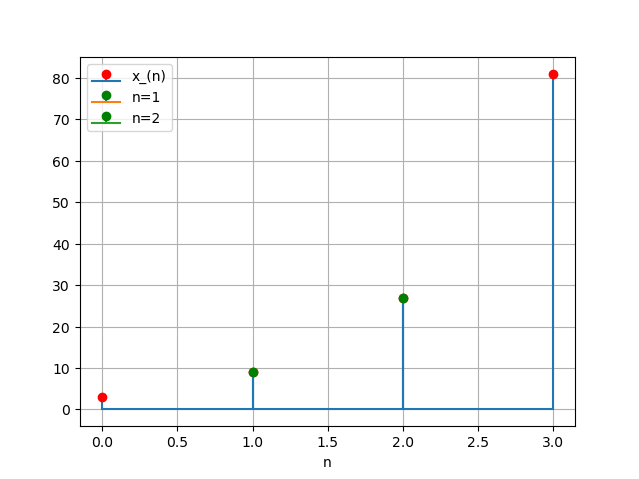
\includegraphics[width = \columnwidth]{ncert-maths/11/9/3/26/figs/Figure_1.png}
    \caption{Graph of $ x\brak{n}$ }
    \label{fig: 11.9.3.26.17}
\end{figure}
\end{enumerate}


\pagebreak

\item  What will Rs 500 amounts to in 10 years after its deposit in a bank which pays annual interest rate of 10$\%$ compounded annually?

\solution
    \let\negmedspace\undefined
\let\negthickspace\undefined
\documentclass[journal,12pt,twocolumn]{IEEEtran}
\usepackage{cite}
\usepackage{amsmath,amssymb,amsfonts,amsthm}
\usepackage{algorithmic}
\usepackage{graphicx}
\usepackage{textcomp}
\usepackage{xcolor}
\usepackage{txfonts}
\usepackage{listings}
\usepackage{enumitem}
\usepackage{mathtools}
\usepackage{gensymb}
\usepackage[breaklinks=true]{hyperref}
\usepackage{tkz-euclide} % loads  TikZ and tkz-base
\usepackage{listings}
\usepackage{gvv}


\newtheorem{theorem}{Theorem}[section]
\newtheorem{problem}{Problem}
\newtheorem{proposition}{Proposition}[section]
\newtheorem{lemma}{Lemma}[section]
\newtheorem{corollary}[theorem]{Corollary}
\newtheorem{example}{Example}[section]
\newtheorem{definition}[problem]{Definition}

\newcommand{\BEQA}{\begin{eqnarray}}
\newcommand{\EEQA}{\end{eqnarray}}
\newcommand{\define}{\stackrel{\triangle}{=}}
\theoremstyle{remark}
\newtheorem{rem}{Remark}

\graphicspath{./figs/}

%\bibliographystyle{ieeetr}
\begin{document}
%

\bibliographystyle{IEEEtran}


\vspace{3cm}

\title{
	%	\logo{
	Assignment-2

	\large{EE:1205 Signals and Systems}

	Indian Institute of Technology, Hyderabad
	%	}
}
\author{Kunal Thorawade

EE23BTECH11035
}	

\maketitle


\newpage

%\tableofcontents

\bigskip
 
 \renewcommand{\thefigure}{\theenumi}
 \renewcommand{\thetable}{\arabic{table}}
 %\renewcommand{\theequation}{\theenumi}

 \section{Question:}
 What will Rs 500 amounts to in 10 years after its deposit in a bank which pays annual interest rate of 10$\%$ compounded annually?

 \section{Solution}

 \begin{table}[ht]
    \centering
    \begin{tabular}{|c|c|c|}
        \hline
        Parameter & Value & Description \\
        \hline
        $x(0)$ & 5 & First term of AP \\
        $d$ & 1.75 & Common difference of AP \\
        $x(n)$ & 20.75 & $n^{th}$ term of AP \\
        \hline
    \end{tabular}
    \vspace{2mm}
    \caption{Parameter List}
    \label{tab:simple.10.5.2.20}
\end{table}


 The Z-transform of a sequence $x(n)$ is given by:

 \begin{align}
	     x(n) &= 500(1.1)^{n}u(n)
	       \\  X(Z) &= \frac{500}{1 - (1.1)z^{-1}} ; |z| > 1.1
 \end{align}

 \begin{figure}
	     \centering
	         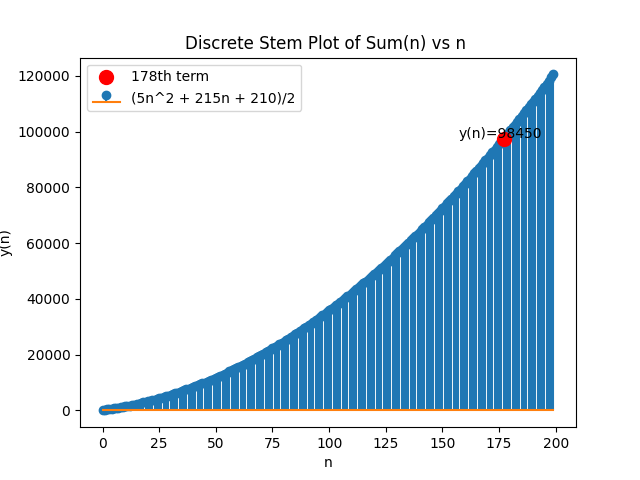
\includegraphics[width = 8cm]{figs/Fig1.png}
		     \caption{Plot of $x(n) = 500(1.1)^n$}
		         \label{fig:enter-label}
 \end{figure}
\end{document}

\pagebreak

\item Find the $20^{th}$ term from the last term of the AP: $3,8,13.....253$.

\solution
% \iffalse
\let\negmedspace\undefined
\let\negthickspace\undefined
\documentclass[journal,12pt,twocolumn]{IEEEtran}
\usepackage{cite}
\usepackage{amsmath,amssymb,amsfonts,amsthm}
\usepackage{algorithmic}
\usepackage{graphicx}
\usepackage{textcomp}
\usepackage{xcolor}
\usepackage{txfonts}
\usepackage{listings}
\usepackage{enumitem}
\usepackage{mathtools}
\usepackage{gensymb}
\usepackage{comment}
\usepackage[breaklinks=true]{hyperref}
\usepackage{tkz-euclide} 
\usepackage{listings}
\usepackage{gvv}                                        
\def\inputGnumericTable{}                                 
\usepackage[latin1]{inputenc}                                
\usepackage{color}                                            
\usepackage{array}                                            
\usepackage{longtable}                                       
\usepackage{calc}                                             
\usepackage{multirow}                                         
\usepackage{hhline}                                           
\usepackage{ifthen}                                           
\usepackage{lscape}
\usepackage{caption}
\newtheorem{theorem}{Theorem}[section]
\newtheorem{problem}{Problem}
\newtheorem{proposition}{Proposition}[section]
\newtheorem{lemma}{Lemma}[section]
\newtheorem{corollary}[theorem]{Corollary}
\newtheorem{example}{Example}[section]
\newtheorem{definition}[problem]{Definition}
\newcommand{\BEQA}{\begin{eqnarray}}
\newcommand{\EEQA}{\end{eqnarray}}
\newcommand{\define}{\stackrel{\triangle}{=}}
\theoremstyle{remark}
\newtheorem{rem}{Remark}
\begin{document}
\parindent 0px
\bibliographystyle{IEEEtran}
\vspace{3cm}

\title{NCERT 10.5.2 17Q}
\author{EE23BTECH11012 - Chavan Dinesh$^{*}$% <-this % stops a space
}
\maketitle
\newpage
\bigskip

\renewcommand{\thefigure}{\arabic{figure}}
\renewcommand{\thetable}{\arabic{table}}
\large\textbf{\textsl{Question:}}
Find the $20^{th}$ term from the last term of the AP: $3,8,13.....253$.

\solution

As the $20^{th}$ term is considered from last, 

\begin{table}[htbp]
    \centering
    \begin{table}[ht]
    \centering
    \begin{tabular}{|c|c|c|}
        \hline
        Parameter & Value & Description \\
        \hline
        $x(0)$ & 5 & First term of AP \\
        $d$ & 1.75 & Common difference of AP \\
        $x(n)$ & 20.75 & $n^{th}$ term of AP \\
        \hline
    \end{tabular}
    \vspace{2mm}
    \caption{Parameter List}
    \label{tab:simple.10.5.2.20}
\end{table}

    \caption{Input table}
    \label{tab:parameter_table.10.5.2.17}
\end{table}
% From \tabref{tab:parameter_table.10.5.2.17}:
% \begin{align}
%     x(n)&=x(0) + nd\\
%      x(19) &= 253 + (-5)19 \\
%         &= 158 
% \end{align}
% From \tabref{tab:parameter_table.10.5.2.17}:
% \begin{align}
% x(N-n)&=x(0) + (N-n)d\\
% x(N-19) &= 3 + (50 - 19)(5)\\
% &= 3 + 155\\
% &= 158
% \end{align}

From equation \eqref{eq:ztrans} and \eqref{eq:11.9.5.26.2}:
% \(Z\)-Transform of \(x(n)\):
\begin{align}
 X(z) =\frac{253}{1-z^{-1}}+ \frac{-5z^{-1}}{\brak{1-z^{-1}}^2};\cbrak{|z|>1}
\end{align}

\begin{figure}[ht]
    \centering
    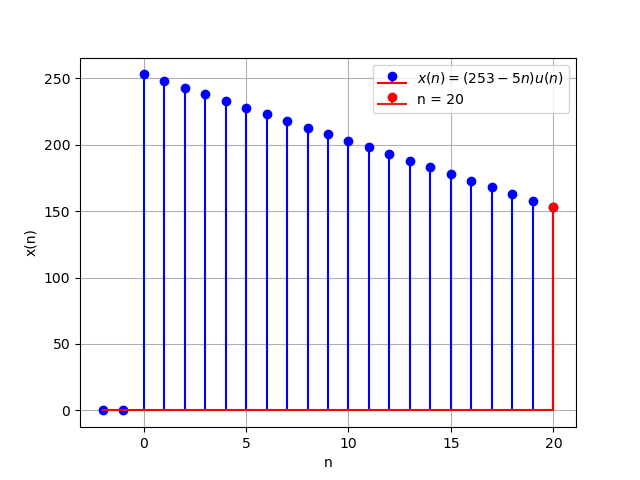
\includegraphics[width = \columnwidth]{figs/x(n)_vs_n.png}
    \caption{}
    \label{fig:graph1.10.5.2.17}
\end{figure}

\bibliographystyle{IEEEtran}
\end{document}


\pagebreak
\item Find the sum to $n$ terms of series , whose $n^{th}$ term is : $n(n+1)(n+4)$.

\solution
\iffalse
\documentclass[journal,12pt,twocolumn]{IEEEtran}
\usepackage{cite}
\usepackage{amsmath,amssymb,amsfonts,amsthm}
\usepackage{algorithmic}
\usepackage{graphicx}
\usepackage{textcomp}
\usepackage{xcolor}
\usepackage{txfonts}
\usepackage{listings}
\usepackage{enumitem}
\usepackage{mathtools}
\usepackage{gensymb}
\usepackage{comment}
\usepackage[breaklinks=true]{hyperref}
\usepackage{tkz-euclide}
\usepackage{listings}
\usepackage{gvv}
\def\inputGnumericTable{}
\usepackage[latin1]{inputenc}
\usepackage{color}
\usepackage{array}
\usepackage{longtable}
\usepackage{calc}
\usepackage{multirow}
\usepackage{hhline}
\usepackage{ifthen}
\usepackage{lscape}
\usepackage{caption}

\newtheorem{theorem}{Theorem}[section]
\newtheorem{problem}{Problem}
\newtheorem{proposition}{Proposition}[section]
\newtheorem{lemma}{Lemma}[section]
\newtheorem{corollary}[theorem]{Corollary}
\newtheorem{example}{Example}[section]
\newtheorem{definition}[problem]{Definition}
\newcommand{\BEQA}{\begin{eqnarray}}
\newcommand{\EEQA}{\end{eqnarray}}
\newcommand{\define}{\stackrel{\triangle}{=}}
\theoremstyle{remark}
\newtheorem{rem}{Remark}
\begin{document}

\bibliographystyle{IEEEtran}
\vspace{3cm}

\title{NCERT 11.9.4 8Q}
\author{EE23BTECH11010 - Venkatesh D Bandawar $^{*}$% <-this % stops a space
}
\maketitle
% \newpage
\bigskip

\renewcommand{\thefigure}{\theenumi}
\renewcommand{\thetable}{\theenumi}

\textbf{Question:} Find the sum to $n$ terms of series , whose $n^{th}$ term is : $n(n+1)(n+4)$.

\textbf{Solution}
\fi
\begin{table}[!h] 
\centering
\begin{tabular}{|c|c|c|}
\hline
\textbf{Parameter} & \textbf{Description} & \textbf{Value} \\
\hline
$x(n)$ & $n^{th}$ term of series & $n(n+1)(n+4)u(n)$\\
\hline
$y(n)$ & sum of n terms of series&\\
\hline
\end{tabular}

\caption{Given parameters}
\label{given parameters list.11.9.4.8}
\end{table}

\begin{align}
        n u(n) &\system{Z} \frac{z^{-1}}{\brak{1-z^{-1}}^2} \cbrak{\abs{z}>1} \label{eq:z transform of nu(n)} \\
        n^2 u(n) &\system{Z} \frac{z^{-1}\brak{1+z^{-1}}}{\brak{1-z^{-1}}^3} \cbrak{\abs{z}>1}\label{eq:z transform of n^2u(n)} \\
        n^3 u(n) &\system{Z} \frac{z^{-1}\brak{1+4z^{-1}+z^{-2}}}{\brak{1-z^{-1}}^4} \cbrak{\abs{z}>1}\label{eq:z transform of n^3u(n)} \\
        n^4 u(n) &\system{Z} \frac{z^{-1}\brak{1+11z^{-1}+11z^{-2}+z^{-3}}}{\brak{1-z^{-1}}^5} \cbrak{\abs{z}>1}\label{eq:z transform of n^4u(n)}
    \end{align}
From equation \eqref{eq:11.9.5.26.2} to \eqref{eq:11.9.5.26.4},\\
    \begin{multline}
        X(z) = \frac{z^{-1}\brak{1+4z^{-1}+z^{-2}}}{\brak{1-z^{-1}}^4} + \frac{5z^{-1}\brak{z^{-1}+1}}{\brak{1-z^{-1}}^3}\\ 
        + \frac{4z^{-1}}{\brak{1-z^{-1}}^2} \cbrak{\abs{z}>1}
    \end{multline}
    \begin{align}
         Y(z) &= X(z)U(z)\\
         &=\frac{z^{-1}\brak{1+4z^{-1}+z^{-2}}}{\brak{1-z^{-1}}^5} + \frac{5z^{-1}\brak{z^{-1}+1}}{\brak{1-z^{-1}}^4} + \frac{4z^{-1}}{\brak{1-z^{-1}}^3} 
    \end{align}
    \begin{multline}
        = \frac{1}{4}\sbrak{\frac{z^{-1}\brak{1+11z^{-1}+11z^{-2}+z^{-3}}}{\brak{1-z^{-1}}^5}} \\
        +\frac{13}{6}\sbrak{\frac{z^{-1}\brak{1+4z^{-1}+z^{-2}}}{\brak{1-z^{-1}}^4}} + \frac{19}{4}\sbrak{\frac{z^{-1}\brak{1+z^{-1}}}{\brak{1-z^{-1}}^3}}\\
        + \frac{17}{6}\sbrak{\frac{z^{-1}}{\brak{1-z^{-1}}^2}} \cbrak{\abs{z}>1}
    \end{multline}
    Taking reverse z transform, using equations \eqref{eq:z transform of nu(n)} to \eqref{eq:z transform of n^4u(n)}
    \begin{align}
        y(n) = \brak{\frac{n^4}{4} + \frac{13n^3}{6} + \frac{19n^2}{4} + \frac{17n}{6}} u\brak{n}
    \end{align}
    \begin{multline}
        = \brak{\frac{n^4}{4} + \frac{2n^3}{4} + \frac{10n^3}{6} + \frac{n^2}{4} + \frac{15n^2}{6} + \frac{4n^2}{2} + \frac{5n}{6} + \frac{4n}{2}} u\brak{n}
    \end{multline}
    \begin{multline}
        = \brak{\frac{n^4+2n^3+n^4}{4}}u\brak{n} +\brak{\frac{10n^3+15n^2+5n}{6}}u\brak{n}\\
        +\brak{\frac{4n^2+4n}{2}}u\brak{n}
    \end{multline}
    \begin{multline}
        = \brak{\frac{n^2\brak{n+1}^2}{4} + \frac{5n(n+1)(2n+1)}{6} 
        + \frac{4n(n+1)}{2}} u\brak{n}
    \end{multline}
    \begin{figure}[!h] 
    \centering
    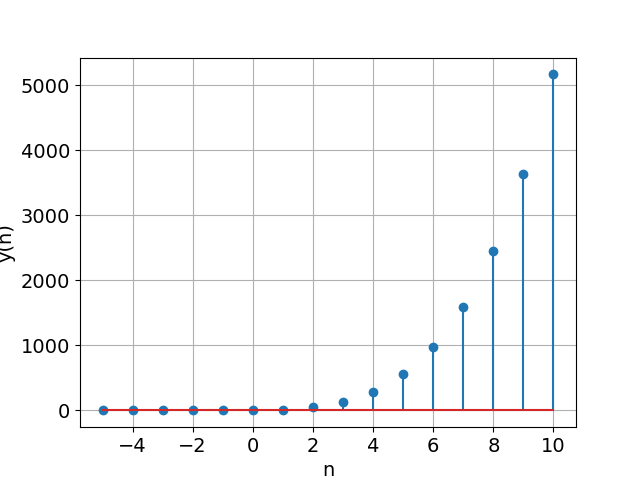
\includegraphics[width=\columnwidth]{ncert-maths/11/9/4/8/figs/sumplot.png}
    \caption{Sum of n terms of series}
    \label{fig:Graph1_math.11.9.4.8}
    \end{figure}


\pagebreak

\item Find the indicated terms in the sequence whose nth terms is $a(n)$ = $4n-3$. Find $a(17)$ and $a(24)$.
    
\solution 
\let\negmedspace\undefined
\let\negthickspace\undefined
\documentclass[journal,12pt,twocolumn]{IEEEtran}

\usepackage{cite}
\usepackage{amsmath,amssymb,amsfonts,amsthm}
\usepackage{algorithmic}
\usepackage{graphicx}
\usepackage{textcomp}
\usepackage{xcolor}
\usepackage{txfonts}
\usepackage{listings}
\usepackage{enumitem}
\usepackage{mathtools}
\usepackage{gensymb}
\usepackage[breaklinks=true]{hyperref}
\usepackage{tkz-euclide} % loads  TikZ and tkz-base
\usepackage{listings}
\usepackage{circuitikz}
\usepackage{graphicx}

%\newcounter{MYtempeqncnt}
\DeclareMathOperator*{\Res}{Res}
%\renewcommand{\baselinestretch}{2}
\renewcommand\thesection{\arabic{section}}
\renewcommand\thesubsection{\thesection.\arabic{subsection}}
\renewcommand\thesubsubsection{\thesubsection.\arabic{subsubsection}}

\renewcommand\thesectiondis{\arabic{section}}
\renewcommand\thesubsectiondis{\thesectiondis.\arabic{subsection}}
\renewcommand\thesubsubsectiondis{\thesubsectiondis.\arabic{subsubsection}}

% correct bad hyphenation here
\hyphenation{op-tical net-works semi-conduc-tor}
\def\inputGnumericTable{}                                 %%

\lstset{
	frame=single,
	breaklines=true,
	columns=fullflexible
}



\newtheorem{theorem}{Theorem}[section]
\newtheorem{problem}{Problem}
\newtheorem{proposition}{Proposition}[section]
\newtheorem{lemma}{Lemma}[section]
\newtheorem{corollary}[theorem]{Corollary}
\newtheorem{example}{Example}[section]
\newtheorem{definition}[problem]{Definition}
\newcommand{\BEQA}{\begin{eqnarray}}
	\newcommand{\EEQA}{\end{eqnarray}}
\newcommand{\define}{\stackrel{\triangle}{=}}
\newcommand\figref{Fig.~\ref}
\newcommand\tabref{Table~\ref}
\bibliographystyle{IEEEtran}
%\bibliographystyle{ieeetr}


\providecommand{\mbf}{\mathbf}
\providecommand{\pr}[1]{\ensuremath{\Pr\left(#1\right)}}
\providecommand{\qfunc}[1]{\ensuremath{Q\left(#1\right)}}
\providecommand{\sbrak}[1]{\ensuremath{{}\left[#1\right]}}
\providecommand{\lsbrak}[1]{\ensuremath{{}\left[#1\right.}}
\providecommand{\rsbrak}[1]{\ensuremath{{}\left.#1\right]}}
\providecommand{\brak}[1]{\ensuremath{\left(#1\right)}}
\providecommand{\lbrak}[1]{\ensuremath{\left(#1\right.}}
\providecommand{\rbrak}[1]{\ensuremath{\left.#1\right)}}
\providecommand{\cbrak}[1]{\ensuremath{\left\{#1\right\}}}
\providecommand{\lcbrak}[1]{\ensuremath{\left\{#1\right.}}
\providecommand{\rcbrak}[1]{\ensuremath{\left.#1\right\}}}
\theoremstyle{remark}
\newtheorem{rem}{Remark}
\newcommand{\sgn}{\mathop{\mathrm{sgn}}}
\providecommand{\abs}[1]{\left\vert#1\right\vert}
\providecommand{\res}[1]{\Res\displaylimits_{#1}}
\providecommand{\norm}[1]{\left\lVert#1\right\rVert}
%\providecommand{\norm}[1]{\lVert#1\rVert}
\providecommand{\mtx}[1]{\mathbf{#1}}
\providecommand{\mean}[1]{E\left[ #1 \right]}
\providecommand{\fourier}{\overset{\mathcal{F}}{ \rightleftharpoons}}
%\providecommand{\hilbert}{\overset{\mathcal{H}}{ \rightleftharpoons}}
\providecommand{\system}{\overset{\mathcal{H}}{ \longleftrightarrow}}
%\newcommand{\solution}[2]{\textbf{Solution:}{#1}}
\newcommand{\solution}{\noindent \textbf{Solution: }}
\newcommand{\cosec}{\,\text{cosec}\,}
\providecommand{\dec}[2]{\ensuremath{\overset{#1}{\underset{#2}{\gtrless}}}}
\newcommand{\myvec}[1]{\ensuremath{\begin{pmatrix}#1\end{pmatrix}}}
\newcommand{\mydet}[1]{\ensuremath{\begin{vmatrix}#1\end{vmatrix}}}
\renewcommand{\abstractname}{Question}

\let\vec\mathbf

	
	\vspace{3cm}
	
	


\newcommand{\permcomb}[4][0mu]{{{}^{#3}\mkern#1#2_{#4}}}
\newcommand{\comb}[1][-1mu]{\permcomb[#1]{C}}

%\IEEEpeerreviewmaketitle

\newcommand \tab [1][1cm]{\hspace*{#1}}
%\newcommand{\Var}{$\sigma ^2$}
\usepackage{amssymb}
\usepackage{amsmath}
\title{
	
\title{NCERT Discrete 11.9.1 Q7}
\author{EE23BTECH11061 - SWATHI DEEPIKA$^{*}$% <-this % stops a space
}


}
\begin{document}

\maketitle

\textbf{Question:} 
Find the indicated terms in the sequence whose nth terms is $a(n)$ = $4n-3$. Find $a(17)$ and $a(24)$.
    
\solution
In the question, following information is provided:
 
 \begin{table}[h]
 	\centering
 	\resizebox{6 cm}{!}{
 		\begin{table}[ht]
    \centering
    \begin{tabular}{|c|c|c|}
        \hline
        Parameter & Value & Description \\
        \hline
        $x(0)$ & 5 & First term of AP \\
        $d$ & 1.75 & Common difference of AP \\
        $x(n)$ & 20.75 & $n^{th}$ term of AP \\
        \hline
    \end{tabular}
    \vspace{2mm}
    \caption{Parameter List}
    \label{tab:simple.10.5.2.20}
\end{table}

 	}
 	\vspace{6 pt}
 	\caption{Parameters}
 	\label{tab:sw_tabel} 
 \end{table}

\begin{align}
x(n) = (4n+1)(u(n))
\end{align}

\begin{align}
 x(16) = 4 \times 16 + 1 = 65
\end{align}

\begin{align}
x(23) = 4 \times 23 + 1 = 93
\end{align}

Using Z-Transform,
\begin{align}
X(z) = 4\frac{z^{-1}}{(1-z^{-1})^2} + \frac{1}{1-z^{-1}}
 \quad |z| > 1
\end{align}

\begin{figure}[!h]
    \centering
    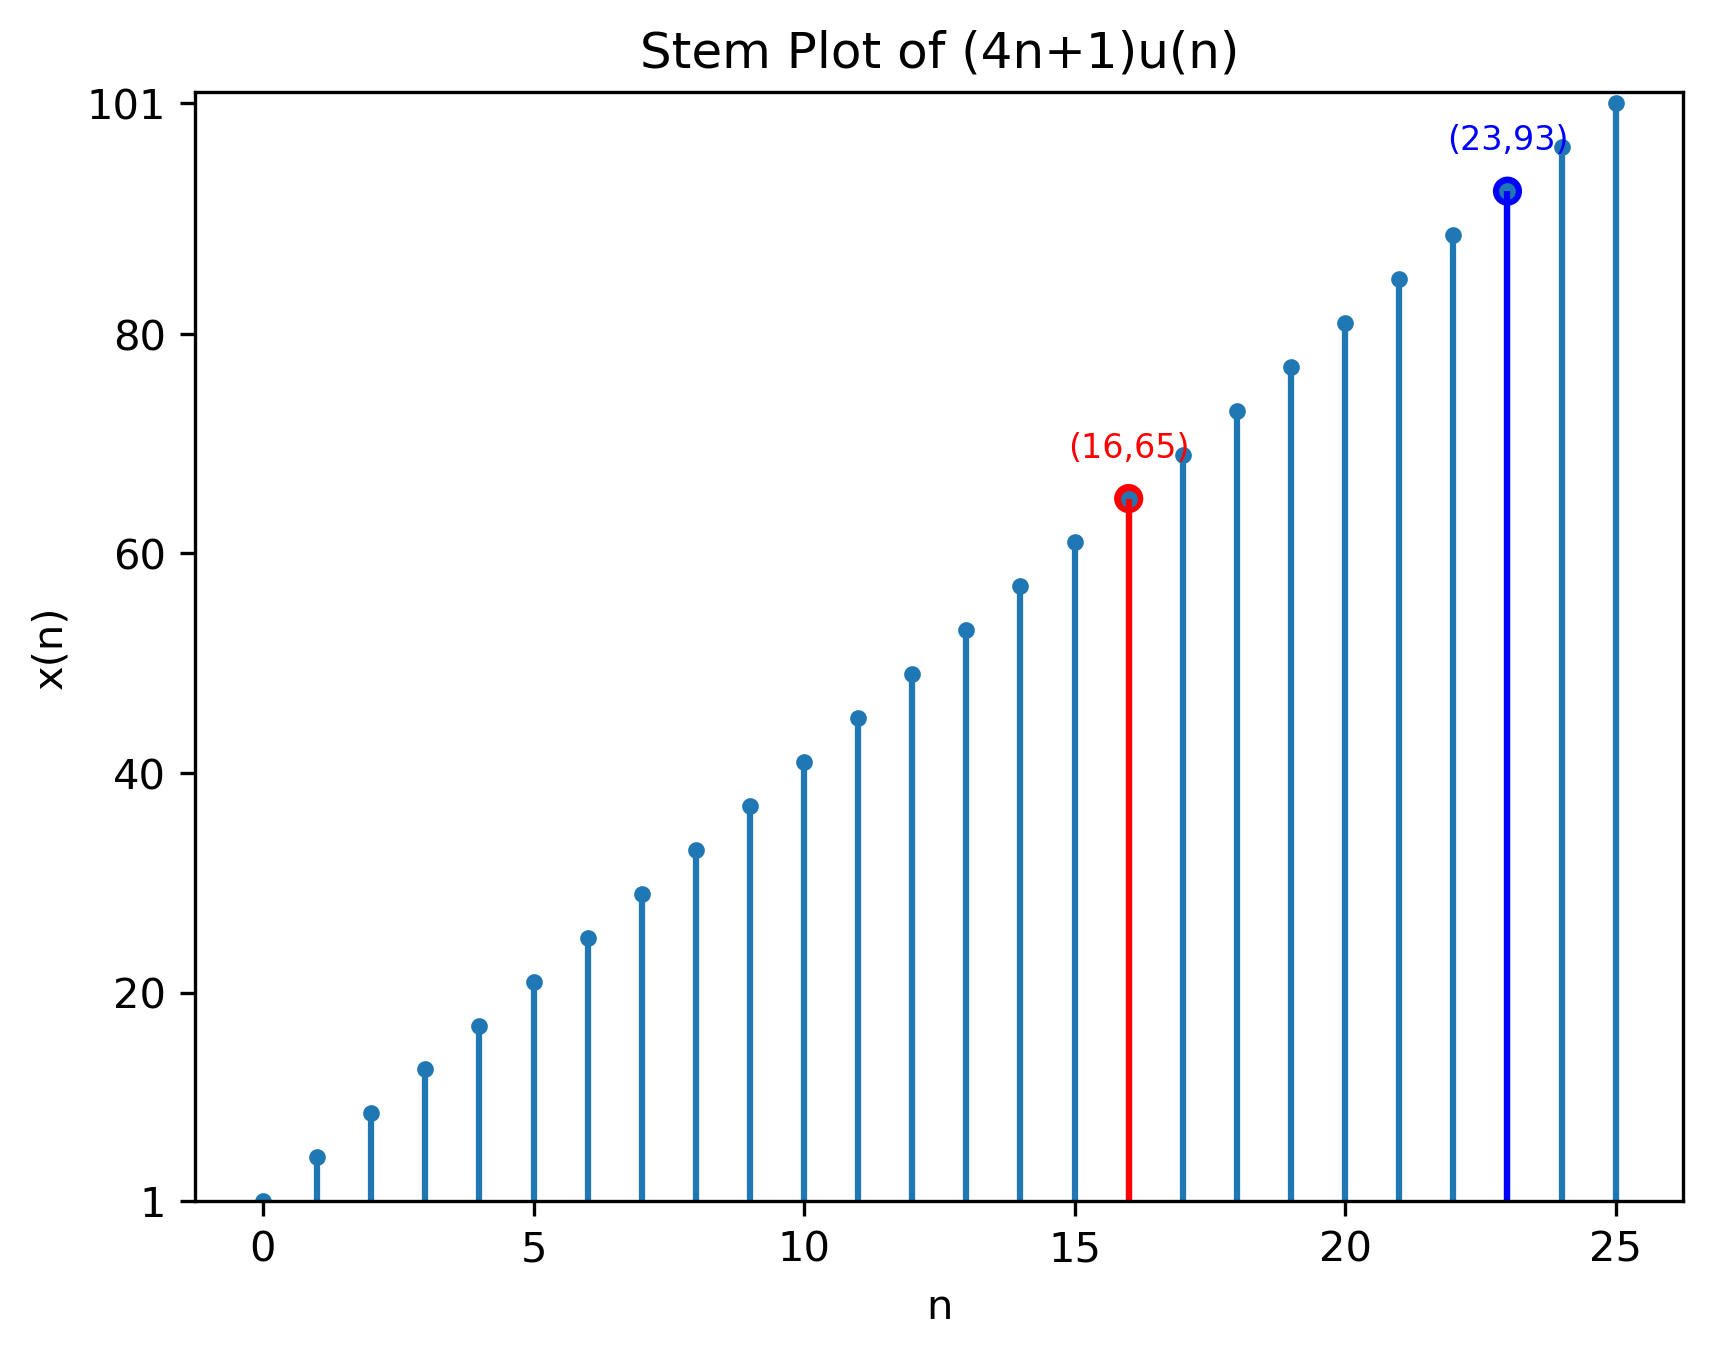
\includegraphics[width = \columnwidth]{figs/a_plot.png}
    \caption{$x(n)$ vs $n$}
    \label{fig:sw_plot}
\end{figure}



\end{document}




\pagebreak

\item The difference between any two cosecutive interior angles of a polygon is $5^\circ$.If the smallest angle is $120^\circ$,find the number of sides of polygon. \\
\solution
\iffalse
\let\negmedspace\undefined
\let\negthickspace\undefined
\documentclass[journal,12pt,twocolumn]{IEEEtran}
\usepackage{cite}
\usepackage{amsmath,amssymb,amsfonts,amsthm}
%\usepackage{algorithmic}
\usepackage{graphicx}
\usepackage{textcomp}
\usepackage{xcolor}
\usepackage{txfonts}
\usepackage{listings}
\usepackage{enumitem}
\usepackage{mathtools}
\usepackage{gensymb}
\usepackage{comment}
\usepackage[breaklinks=true]{hyperref}
\usepackage{tkz-euclide} % loads  TikZ and tkz-base
\usepackage{listings}
\usepackage[latin1]{inputenc}                                
\usepackage{color}                                            
\usepackage{array}                                            
\usepackage{longtable}                                       
\usepackage{calc}                                             
\usepackage{multirow}                                         
\usepackage{hhline}                                           
\usepackage{ifthen}                                           
\usepackage{lscape}
\usepackage{caption}
\usepackage{gvv}

\newtheorem{theorem}{Theorem}[section]
\newtheorem{problem}{Problem}
\newtheorem{proposition}{Proposition}[section]
\newtheorem{lemma}{Lemma}[section]
\newtheorem{corollary}[theorem]{Corollary}
\newtheorem{example}{Example}[section]
\newtheorem{definition}[problem]{Definition}
%\newtheorem{thm}{Theorem}[section] 
%\newtheorem{defn}[thm]{Definition}
%\newtheorem{algorithm}{Algorithm}[section]
%\newtheorem{cor}{Corollary}
\newcommand{\BEQA}{\begin{eqnarray}}
\newcommand{\system}[1]{\stackrel{#1}{\rightarrow}}
\newcommand{\EEQA}{\end{eqnarray}}
\newcommand{\define}{\stackrel{\triangle}{=}}
\theoremstyle{remark}
\newtheorem{rem}{Remark}
%\bibliographystyle{ieeetr}

\begin{document}
\providecommand{\pr}[1]{\ensuremath{\Pr\left(#1\right)}}
\providecommand{\prt}[2]{\ensuremath{p_{#1}^{\left(#2\right)} }}        % own macro for this question
\providecommand{\qfunc}[1]{\ensuremath{Q\left(#1\right)}}
\providecommand{\sbrak}[1]{\ensuremath{{}\left[#1\right]}}
\providecommand{\lsbrak}[1]{\ensuremath{{}\left[#1\right.}}
\providecommand{\rsbrak}[1]{\ensuremath{{}\left.#1\right]}}
\providecommand{\brak}[1]{\ensuremath{\left(#1\right)}}
\providecommand{\lbrak}[1]{\ensuremath{\left(#1\right.}}
\providecommand{\rbrak}[1]{\ensuremath{\left.#1\right)}}
\providecommand{\cbrak}[1]{\ensuremath{\left\{#1\right\}}}
\providecommand{\lcbrak}[1]{\ensuremath{\left\{#1\right.}}
\providecommand{\rcbrak}[1]{\ensuremath{\left.#1\right\}}}
\newcommand{\sgn}{\mathop{\mathrm{sgn}}}
\providecommand{\abs}[1]{\left\vert#1\right\vert}
\providecommand{\res}[1]{\Res\displaylimits_{#1}} 
\providecommand{\norm}[1]{\left\lVert#1\right\rVert}
%\providecommand{\norm}[1]{\lVert#1\rVert}
\providecommand{\mtx}[1]{\mathbf{#1}}
\providecommand{\mean}[1]{E\left[ #1 \right]}
\providecommand{\cond}[2]{#1\middle|#2}
\providecommand{\fourier}{\overset{\mathcal{F}}{ \rightleftharpoons}}
\newenvironment{amatrix}[1]{%
  \left(\begin{array}{@{}*{#1}{c}|c@{}}
}{%
  \end{array}\right)
}
%\providecommand{\hilbert}{\overset{\mathcal{H}}{ \rightleftharpoons}}
%\providecommand{\system}{\overset{\mathcal{H}}{ \longleftrightarrow}}
        %\newcommand{\solution}[2]{\textbf{Solution:}{#1}}
\newcommand{\solution}{\noindent \textbf{Solution: }}
\newcommand{\cosec}{\,\text{cosec}\,}
\providecommand{\dec}[2]{\ensuremath{\overset{#1}{\underset{#2}{\gtrless}}}}
\newcommand{\myvec}[1]{\ensuremath{\begin{pmatrix}#1\end{pmatrix}}}
\newcommand{\mydet}[1]{\ensuremath{\begin{vmatrix}#1\end{vmatrix}}}
\newcommand{\myaugvec}[2]{\ensuremath{\begin{amatrix}{#1}#2\end{amatrix}}}
\providecommand{\rank}{\text{rank}}
\providecommand{\pr}[1]{\ensuremath{\Pr\left(#1\right)}}
\providecommand{\qfunc}[1]{\ensuremath{Q\left(#1\right)}}
        \newcommand*{\permcomb}[4][0mu]{{{}^{#3}\mkern#1#2_{#4}}}
\newcommand*{\perm}[1][-3mu]{\permcomb[#1]{P}}
\newcommand*{\comb}[1][-1mu]{\permcomb[#1]{C}}
\providecommand{\qfunc}[1]{\ensuremath{Q\left(#1\right)}}
\providecommand{\gauss}[2]{\mathcal{N}\ensuremath{\left(#1,#2\right)}}
\providecommand{\diff}[2]{\ensuremath{\frac{d{#1}}{d{#2}}}}
\providecommand{\myceil}[1]{\left \lceil #1 \right \rceil }
\newcommand\figref{Fig.~\ref}
\newcommand\tabref{Table~\ref}
\newcommand{\sinc}{\,\text{sinc}\,}
\newcommand{\rect}{\,\text{rect}\,}
%%
%       %\newcommand{\solution}[2]{\textbf{Solution:}{#1}}
%\newcommand{\solution}{\noindent \textbf{Solution: }}
%\newcommand{\cosec}{\,\text{cosec}\,}
%\numberwithin{equation}{section}
%\numberwithin{equation}{subsection}
%\numberwithin{problem}{section}
%\numberwithin{definition}{section}
%\makeatletter
%\@addtoreset{figure}{problem}
%\makeatother

%\let\StandardTheFigure\thefigure
\let\vec\mathbf

\bibliographystyle{IEEEtran}

\vspace{3cm}
\title{Assignment}
\author{EE23BTECH11008 - Meenakshi}
\maketitle
\newpage
\bigskip

\renewcommand{\thefigure}{\theenumi}
\renewcommand{\thetable}{\theenumi}
%\renewcommand{\theequation}{\theenumi}
Q:The difference between any two cosecutive interior angles of a polygon is $5^\circ$.If the smallest angle is $120^\circ$,find the number of sides of polygon. \\
\solution
\fi
\begin{table}[!ht]
    \centering
         \begin{tabular}{|c|c|c|} 
      \hline
\textbf{Variable}& \textbf{Description}& \textbf{Value}\\\hline
$x(0)$& first term of AP& 120  \\\hline
    d& common difference of AP & 5\\\hline
    $x(n)$ & general  term of AP&none\\\hline
\end{tabular}

    \caption{input parameters}
    \label{tab:11_9_2_1}
\end{table}

Sum of interior angles of a polygon with $n+1$ sides is given by
\begin{align}
    S &= (n-1)180
\end{align}
Sum of $n$ terms of AP is given by
\begin{align}
    y(n) &= x(n)*u(n)
\end{align}
where $x(n) = 120 + 5n$
\begin{equation}
    x(n)*u(n)=(n-1)180 \label{eq:11.9.2.4.eq}
\end{equation}
\begin{align}
    Y(z) &= X(z)U(z) \\
    &= \left(\frac{x(0)}{1-z^{-1}} + \frac{dz^{-1}}{(1-z^{-1})^2}\right) \frac{1}{1-z^{-1}} \quad |z|>1\\
    &=\frac{120}{(1-z^{-1})^2} + \frac{5z^{-1}}{(1-z^{-1})^3} \quad |z|>1
\end{align}
\begin{align}
	\brak{n+1}u\brak{n}&\system{ Z}\left(\frac{1}{\brak{1-z^{-1}}^2}\right)\quad |z|>1\label{eq:11.9.2.18.9} \\
	\frac{\brak{n}\brak{n-1}}{2}u\brak{n-1} &\system{Z}\left(\frac{z^{-1}}{\brak{1-z^{-1}}^3}\right) \quad |z|>1\label{eq:11.9.2.18.10}
\end{align}
applying inverse Z-transform for each term and solving we get,
\begin{align}
    y\brak{n} &= \frac{n+1}{2}\brak{240+5n}u(n)
\end{align}
now from ~\eqref{eq:11.9.2.4.eq} 
\begin{align}
y(n) &= (n-1)180 \\
\frac{n+1}{2}\brak{240+5n}u(n) &= (n-1)180
\end{align}
now replace $n$ by $n-1$: 
\begin{align}
    n(235+5n) &= (n-2)360\\
    5n^2-125n+720 &= 0
\end{align}
\begin{align}
   n &= 16,9
\end{align}

\begin{figure}[h]
\centering
 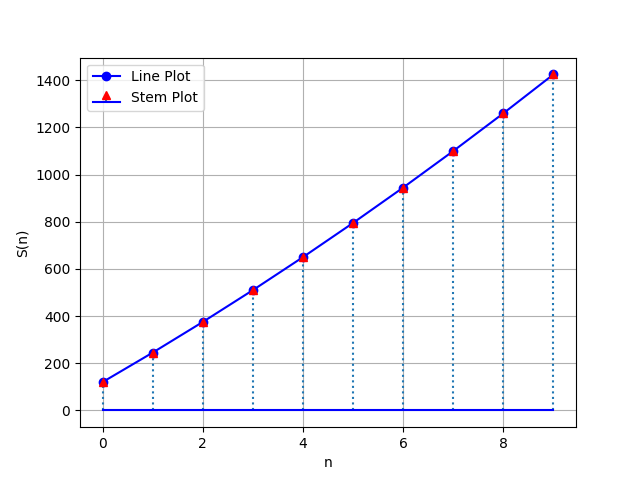
\includegraphics[width=\columnwidth]{ncert-maths/11/9/2/18/figs/python.1(1).png} 
  \captionsetup{justification=centering}
  \caption{Plot of the sum of n terms taken from Python}
  \label{fig:your_label}
\end{figure}

%\end{document}
   
   




\pagebreak
\item The $5$th,$8$th and $11$th terms of a GP are p,q and s respectively .show that $q^2=ps$ \\
\solution
\iffalse
\let\negmedspace\undefined
\let\negthickspace\undefined
\documentclass[journal,12pt,twocolumn]{IEEEtran}
\usepackage{cite}
\usepackage{amsmath,amssymb,amsfonts,amsthm}
\usepackage{algorithmic}
\usepackage{graphicx}
\usepackage{textcomp}
\usepackage{xcolor}
\usepackage{txfonts}
\usepackage{listings}
\usepackage{enumitem}
\usepackage{mathtools}
\usepackage{gensymb}
\usepackage{comment}
\usepackage[breaklinks=true]{hyperref}
\usepackage{tkz-euclide} 
\usepackage{listings}
\usepackage{gvv}                                        
\def\inputGnumericTable{}                                 
\usepackage[latin1]{inputenc}                                
\usepackage{color}                                            
\usepackage{array}                                            
\usepackage{longtable}                                       
\usepackage{calc}                                             
\usepackage{multirow}                                         
\usepackage{hhline}                                           
\usepackage{ifthen}                                           
\usepackage{lscape}

\newtheorem{theorem}{Theorem}[section]
\newtheorem{problem}{Problem}
\newtheorem{proposition}{Proposition}[section]
\newtheorem{lemma}{Lemma}[section]
\newtheorem{corollary}[theorem]{Corollary}
\newtheorem{example}{Example}[section]
\newtheorem{definition}[problem]{Definition}
\newcommand{\BEQA}{\begin{eqnarray}}
\newcommand{\EEQA}{\end{eqnarray}}
\newcommand{\define}{\stackrel{\triangle}{=}}
\theoremstyle{remark}
\newtheorem{rem}{Remark}
\begin{document}

\bibliographystyle{IEEEtran}
\vspace{3cm}

\title{11.9.3.3}
\author{EE23BTECH11065 - prem sagar}
\maketitle
\newpage

\bigskip 

\renewcommand{\thefigure}{\theenumi}
\renewcommand{\thetable}{\theenumi}
\textbf{Question}:\\ The $5$th,$8$th and $11$th terms of a GP are p,q and s respectively .show that $q^2=ps$
\\\\\textbf{solution}:
\fi
\begin{table}[!ht]
   \centering
    \renewcommand\thetable{1}
      \begin{tabular}{|c|c|c|}
    \hline
            \textbf{Symbol} & \textbf{Value} & \textbf{Description} \\
    \hline
          $x\brak{5}$ & $p$ & $x\brak{0}r^5$ \\
    \hline
          $x\brak{8}$ & $q$ & $x\brak{0}r^8$\\
    \hline 
          $x\brak{{11}}$ &$s$ &$x\brak{0}r^{11}$ \\
    \hline
          $x\brak{n}$ & &$x\brak{0}r^nu\brak{n}$ \\
    \hline
          $r$& $\brak{\frac{s}{p}}^\frac{1}{6}$& common ratio\\
     \hline     
  \end{tabular}

    \caption{input parameters}
    \label{tab:11.9.3}
 \end{table}
\\ From \tabref{tab:11.9.3}:
\begin{align}
q^2&=x\brak{0}\,r^8\,x\brak{0}\,r^8
     \\ &=x\brak{0}^2\,r^{16}
\\ps&=x\brak{0}\,r^5\,x(0)\,r^{11}
       \\&=x\brak{0}^2\,r^{16}
\\\implies q^2&=ps
\end{align}
now we will find r and x\brak{0}:
\begin{align}
\frac{s}{p}&=\frac{x\brak{0}r^{11}}{x\brak{0}r^5}
\\r&=\brak{\frac{s}{p}}^\frac{1}{6} 
\\p&=x\brak{0}\brak{\frac{s}{p}}^\frac{5}{6}
\\x\brak{0}&=\frac{p^\frac{11}{6}}{s^\frac{5}{6}}
\end{align}
Applying z-Transform:
\begin{align}
     X(z) &= \frac{x\brak{0}}{1-r\,z^{-1}}\: \:,\abs{z}>\abs{r}
\\ \implies  X(z)&=\frac{p^3}{p^\frac{7}{6}s^\frac{5}{6}-q^2z^{-1}}\:,\abs{z}>\abs{\brak{\frac{q}{p}}^\frac{1}{3}}
     \end{align}    
\\\begin{figure}[h]
   \renewcommand\thefigure{1}
    \centering
    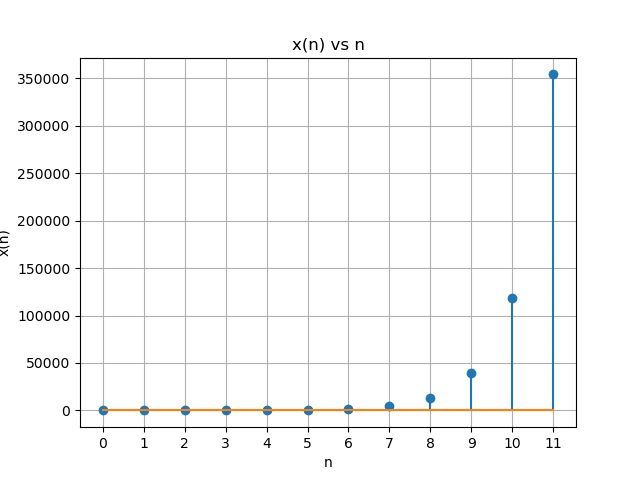
\includegraphics[width=1\linewidth]{/root/assign1/figs/figure__plot.png}
    \caption{plot x\brak{n}vs n\hspace{0.1cm}$p=486$,
    \hspace{0.1cm}$q=13122$,
    \hspace{0.1cm}$s=354294$,
    \hspace{0.1cm}$r=3$}
    \label{fig:1}
\end{figure}\\
\end{document}

\pagebreak
\item The sum of the first four terms of an A.P. is 56. The sum of the last four terms is
 112. If its first term is 11, then find the number of terms.\\
\solution
\iffalse
\let\negmedspace\undefined
\let\negthickspace\undefined
\documentclass[journal,12pt,twocolumn]{IEEEtran}
\usepackage{cite}
\usepackage{amsmath,amssymb,amsfonts,amsthm}
\usepackage{algorithmic}
\usepackage{graphicx}
\usepackage{textcomp}
\usepackage{xcolor}
\usepackage{txfonts}
\usepackage{listings}
\usepackage{enumitem}
\usepackage{mathtools}
\usepackage{gensymb}
\usepackage{comment}
\usepackage[breaklinks=true]{hyperref}
\usepackage{tkz-euclide} 
\use-package{listings}
\usepackage{gvv}                                        
\def\inputGnumericTable{}                                 
\usepackage[latin1]{inputenc}                                
\usepackage{color}                                            
\usepackage{array}                                            
\usepackage{longtable}                                       
\usepackage{calc}                                             
\usepackage{multirow}                                         
\usepackage{hhline}                                           
\usepackage{ifthen}                                           
\usepackage{lscape}
\usepackage{caption}

\newtheorem{theorem}{Theorem}[section]
\newtheorem{problem}{Problem}
\newtheorem{proposition}{Proposition}[section]
\newtheorem{lemma}{Lemma}[section]
\newtheorem{corollary}[theorem]{Corollary}
\newtheorem{example}{Example}[section]
\newtheorem{definition}[problem]{Definition}
\newcommand{\BEQA}{\begin{eqnarray}}
\newcommand{\EEQA}{\end{eqnarray}}
\newcommand{\define}{\stackrel{\triangle}{=}}
\theoremstyle{remark}
\newtheorem{rem}{Remark}
\begin{document}

\bibliographystyle{IEEEtran}
\vspace{3cm}

\title{11.9.5}
\author{EE23BTECH11029 - Kanishk}
\maketitle

\bigskip


\textbf{Question}:\\ 
The sum of the first four terms of an A.P. is 56. The sum of the last four terms is
112. If its first term is 11, then find the number of terms.\\

\textbf{Solution}:\\ 
\fi
\begin{table}[ht]
    \centering
    \def\arraystretch{1.5}
    \footnotesize
\begin{tabular}{|c|c|c|}
\hline
Symbol & Value & Description\\
\hline
$x(0)$ & $11$ & First term of AP \\
\hline
$y\brak{3}$ & $56$ & Sum of the first four terms of AP\\
\hline
$y\brak{n}-y\brak{n-4}$ & $112$& Sum of the last four terms of AP\\
\hline
\end{tabular}

   \caption{Input Parameters}
   \label{tab:11.9.5.12}
\end{table}

\small
\begin{align}
y\brak{n}&=\sbrak{\frac{\brak{n+1}}{2}\brak{2x\brak{0}+nd}}u\brak{n}\\
\implies y(3)&=\frac{4}{2}\brak{2x\brak{0}+3d}\\
\end{align}
From \tabref{tab:11.9.5.12}:
\begin{align}
\frac{4}{2}\brak{2x\brak{0}+3d}&=56\\
2x\brak{0}+3d&=28\\
\implies d&=2
\end{align}

\begin{align}
 y\brak{n}-y\brak{n-4}&=\frac{4}{2}\brak{2x\brak{n}+3\brak{-d}}
\end{align}
From \tabref{tab:11.9.5.12}:
\begin{align}
\frac{4}{2}\brak{2x\brak{n}+3\brak{-d}}&=112\\
2x\brak{n}-3d&=56\\
\implies x\brak{n}&=31\\
x\brak{0}+\brak{n}2&=31\\
\implies n&=10
\end{align}


\begin{align}
x\brak{n}&=\brak{x\brak{0}+2n}u\brak{n}\\
\implies X\brak{z}&=\frac{x\brak{0}}{1-z^{-1}}+2\frac{z^{-1}}{\brak{1-z^{-1}}^{2}}.\quad \abs{z} > 1
\end{align}

\newpage

\begin{figure}
    
    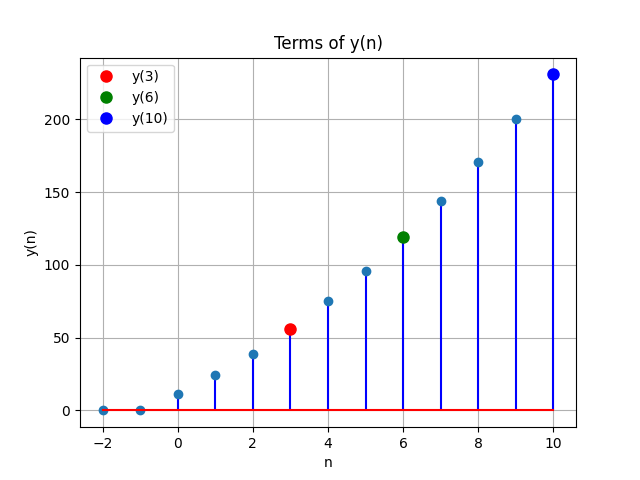
\includegraphics[width=\columnwidth]{ncert-maths/11/9/5/12//figs/fig1.png}
    \caption{Plot y(n) vs n}
\end{figure}

%\end{document}
\pagebreak
\item Find the sum to $n$ terms of the series whose $n^{th}$ term is given by $(2n-1)^2$ ? 
\solution
\iffalse
\let\negmedspace\undefined
\let\negthickspace\undefined
\documentclass[journal,12pt,onecolumn]{IEEEtran}
\usepackage{cite}
\usepackage{amsmath,amssymb,amsfonts,amsthm}
\usepackage{algorithmic}
\usepackage{graphicx}
\usepackage{textcomp}
\usepackage{xcolor}
\usepackage{txfonts}
\usepackage{listings}
\usepackage{enumitem}
\usepackage{mathtools}
\usepackage{gensymb}
\usepackage[breaklinks=true]{hyperref}
\usepackage{tkz-euclide} % loads  TikZ and tkz-base
\usepackage{listings}



\newtheorem{theorem}{Theorem}[section]
\newtheorem{problem}{Problem}
\newtheorem{proposition}{Proposition}[section]
\newtheorem{lemma}{Lemma}[section]
\newtheorem{corollary}[theorem]{Corollary}
\newtheorem{example}{Example}[section]
\newtheorem{definition}[problem]{Definition}
%\newtheorem{thm}{Theorem}[section] 
%\newtheorem{defn}[thm]{Definition}
%\newtheorem{algorithm}{Algorithm}[section]
%\newtheorem{cor}{Corollary}
\newcommand{\BEQA}{\begin{eqnarray}}
\newcommand{\EEQA}{\end{eqnarray}}
\newcommand{\system}[1]{\stackrel{#1}{\rightarrow}}
\newcommand{\define}{\stackrel{\triangle}{=}}
\theoremstyle{remark}
\newtheorem{rem}{Remark}
%\bibliographystyle{ieeetr}
\begin{document}
%
\providecommand{\pr}[1]{\ensuremath{\Pr\left(#1\right)}}
\providecommand{\prt}[2]{\ensuremath{p_{#1}^{\left(#2\right)} }}        % own macro for this question
\providecommand{\qfunc}[1]{\ensuremath{Q\left(#1\right)}}
\providecommand{\sbrak}[1]{\ensuremath{{}\left[#1\right]}}
\providecommand{\lsbrak}[1]{\ensuremath{{}\left[#1\right.}}
\providecommand{\rsbrak}[1]{\ensuremath{{}\left.#1\right]}}
\providecommand{\brak}[1]{\ensuremath{\left(#1\right)}}
\providecommand{\lbrak}[1]{\ensuremath{\left(#1\right.}}
\providecommand{\rbrak}[1]{\ensuremath{\left.#1\right)}}
\providecommand{\cbrak}[1]{\ensuremath{\left\{#1\right\}}}
\providecommand{\lcbrak}[1]{\ensuremath{\left\{#1\right.}}
\providecommand{\rcbrak}[1]{\ensuremath{\left.#1\right\}}}
\newcommand{\sgn}{\mathop{\mathrm{sgn}}}
\providecommand{\abs}[1]{\left\vert#1\right\vert}
\providecommand{\res}[1]{\Res\displaylimits_{#1}} 
\providecommand{\norm}[1]{\left\lVert#1\right\rVert}
%\providecommand{\norm}[1]{\lVert#1\rVert}
\providecommand{\mtx}[1]{\mathbf{#1}}
\providecommand{\mean}[1]{E\left[ #1 \right]}
\providecommand{\cond}[2]{#1\middle|#2}
\providecommand{\fourier}{\overset{\mathcal{F}}{ \rightleftharpoons}}
\newenvironment{amatrix}[1]{%
  \left(\begin{array}{@{}*{#1}{c}|c@{}}
}{%
  \end{array}\right)
}
%\providecommand{\hilbert}{\overset{\mathcal{H}}{ \rightleftharpoons}}
%\providecommand{\system}{\overset{\mathcal{H}}{ \longleftrightarrow}}
	%\newcommand{\solution}[2]{\textbf{Solution:}{#1}}
\newcommand{\solution}{\noindent \textbf{Solution: }}
\newcommand{\cosec}{\,\text{cosec}\,}
\providecommand{\dec}[2]{\ensuremath{\overset{#1}{\underset{#2}{\gtrless}}}}
\newcommand{\myvec}[1]{\ensuremath{\begin{pmatrix}#1\end{pmatrix}}}
\newcommand{\mydet}[1]{\ensuremath{\begin{vmatrix}#1\end{vmatrix}}}
\newcommand{\myaugvec}[2]{\ensuremath{\begin{amatrix}{#1}#2\end{amatrix}}}
\providecommand{\rank}{\text{rank}}
\providecommand{\pr}[1]{\ensuremath{\Pr\left(#1\right)}}
\providecommand{\qfunc}[1]{\ensuremath{Q\left(#1\right)}}
	\newcommand*{\permcomb}[4][0mu]{{{}^{#3}\mkern#1#2_{#4}}}
\newcommand*{\perm}[1][-3mu]{\permcomb[#1]{P}}
\newcommand*{\comb}[1][-1mu]{\permcomb[#1]{C}}
\providecommand{\qfunc}[1]{\ensuremath{Q\left(#1\right)}}
\providecommand{\gauss}[2]{\mathcal{N}\ensuremath{\left(#1,#2\right)}}
\providecommand{\diff}[2]{\ensuremath{\frac{d{#1}}{d{#2}}}}
\providecommand{\myceil}[1]{\left \lceil #1 \right \rceil }
\newcommand\figref{Fig.~\ref}
\newcommand\tabref{Table~\ref}
\newcommand{\sinc}{\,\text{sinc}\,}
\newcommand{\rect}{\,\text{rect}\,}
%%
%	%\newcommand{\solution}[2]{\textbf{Solution:}{#1}}
%\newcommand{\solution}{\noindent \textbf{Solution: }}
%\newcommand{\cosec}{\,\text{cosec}\,}
%\numberwithin{equation}{section}
%\numberwithin{equation}{subsection}
%\numberwithin{problem}{section}
%\numberwithin{definition}{section}
%\makeatletter
%\@addtoreset{figure}{problem}
%\makeatother

%\let\StandardTheFigure\thefigure
\let\vec\mathbf


\bibliographystyle{IEEEtran}
\title{SEQUENCE AND SERIES}
\author{EE23BTECH11011- Batchu Ishitha$^{*}$% <-this % stops a space
}
\maketitle




\bigskip

\renewcommand{\thefigure}{\theenumi}
\renewcommand{\thetable}{\theenumi}
%\renewcommand{\theequation}{\theenumi}

Q: Find the sum to $n$ terms of the series whose $n^{th}$ term is given by $(2n-1)^2$ ?

\solution
\fi
\begin{table}[!ht]
    \centering
        
      \begin{tabular}{|c|c|c|} 
      \hline
\textbf{Variable}& \textbf{Description}& \textbf{Value}\\\hline
         $x(n)$& $n^{th}$ term of sequence& $(2n+1)^2u(n)$\\\hline
          
    \end{tabular}


    \caption{input parameters}
    \label{}
\end{table}
Sum of $n$ terms of AP is given by
\begin{align}
 y(n)&=x(n)*u(n) \\
x(n)&= (2n+1)^2 u(n) 
\end{align}

\begin{equation}
   u(n) \xleftrightarrow{\mathcal{Z}} \frac{1}{(1-z^{-1})}  \quad \abs{z}>1\\ \label{eq:11.9.4.10.1.eq}
\end{equation}

\begin{equation}   
   nu(n) \xleftrightarrow{\mathcal{Z}} \frac{z^{-1}}{(1-z^{-1})^2} \quad \abs{z}>1\\ \label{eq:11.9.4.10.2.eq}
\end{equation}

\begin{equation}   
   n^2u(n) \xleftrightarrow{\mathcal{Z}} \frac{z^{-1}(1+z^{-1})}{(1-z^{-1})^3} \quad \abs{z}>1 \\ \label{eq:11.9.4.10.3.eq}
\end{equation}  

\begin{equation}
n^3u(n) \xleftrightarrow{\mathcal{Z}} \frac{z^{-1}\brak{1+4z^{-1}+z^{-2}}}{\brak{1-z^{-1}}^4} \quad \abs{z}>1 \\ \label{eq:11.9.4.10.4.eq}
\end{equation} 
 
\begin{align}
\implies  X(z)&=\frac{4z^{-1}(1+z^{-1})}{(1-z^{-1})^3} + \frac{1}{(1-z^{-1})} + \frac{4z^{-1}}{(1-z^{-1})^2} \quad \abs{z}>1 \\
 Y(z) &= X(z)U(z) \\
 &= \brak{\frac{4z^{-1}(z^{-1}+1)}{(1-z^{-1})^3} + \frac{1}{(1-z^{-1})} + \frac{4z^{-1}}{(1-z^{-1})^2}}\brak{\frac{1}{1-z^{-1}}}\\
 &= \frac{4z^{-1}(z^{-1}+1)}{(1-z^{-1})^4} + \frac{1}{(1-z^{-1})^2} + \frac{4z^{-1}}{(1-z^{-1})^3}
 \end{align}
 
 \begin{equation}
\implies Y(Z)=\frac{1}{(1-z^{-1})} +\frac{9z^{-1}}{(1-z^{-1})} + \frac{25z^{-2}}{(1-z^{-1})^2} + \frac{24z^{-3}}{(1-z^{-1})^3} + \frac{8z^{-4}}{(1-z^{-1})^4} \quad \abs{z}>1  \label{eq:11.9.4.10.5.eq}
 \end{equation}
Now from~\eqref{eq:11.9.4.10.1.eq},~\eqref{eq:11.9.4.10.2.eq},~\eqref{eq:11.9.4.10.3.eq},~\eqref{eq:11.9.4.10.4.eq},
 ~\eqref{eq:11.9.4.10.5.eq}
By using  inverse Z-transform pairs,
\begin{align}
  y\brak{n}&= u(n) + 9u(n-1) + 25(n-1)u(n-2) + 24\frac{(n-1)(n-2)}{2}u(n-3) + 8\frac{(n-1)(n-2)(n-3)}{6}u(n-4) \\
\implies  y\brak{n} &=\brak{\frac{4n^{3}+12n^{2}+11n+3}{3}}u(n)
\end{align}
$\therefore$ Sum of $n$ terms of the series whose $n^{th}$ term is given by $(2n+1)^2$ is $\frac{4n^{3}+12n^{2}+11n+3}{3}$  .
\begin{figure}[h]
    \centering
     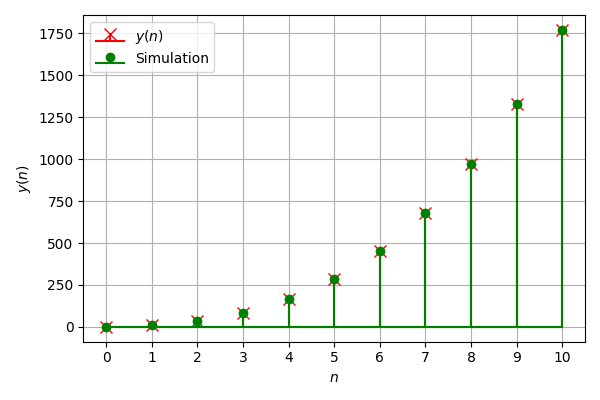
\includegraphics[width=\columnwidth]{ncert-maths/11/9/4/10/figs/fig2.png}
    \caption{Theory vs Simulation}    
    \label{}
\end{figure}


%\end{document}


\pagebreak
\item If the $4^{th}$, $10^{th}$ and $16^{th}$ terms of a G.P. are $x$, $y$, and $z$, respectively. Prove that $x,\; y,\; z$ are in G.P. \\
\solution
\iffalse
\let\negmedspace\undefined
\let\negthickspace\undefined
\documentclass[journal,12pt,twocolumn]{IEEEtran}
\usepackage{cite}
\usepackage{amsmath,amssymb,amsfonts,amsthm}
\usepackage{algorithmic}
\usepackage{graphicx}
\usepackage{textcomp}
\usepackage{xcolor}
\usepackage{txfonts}
\usepackage{listings}
\usepackage{enumitem}
\usepackage{mathtools}
\usepackage{gensymb}
\usepackage{comment}
\usepackage[breaklinks=true]{hyperref}
\usepackage{tkz-euclide} 
\usepackage{listings}
\usepackage{gvv}                                        
%\def\inputGnumericTable{}                                 
\usepackage[latin1]{inputenc}                                
\usepackage{color}                                            
\usepackage{array}                                            
\usepackage{longtable}                                       
\usepackage{calc}                                             
\usepackage{multirow}                                         
\usepackage{hhline}                                           
\usepackage{ifthen}                                           
\usepackage{lscape}
\usepackage{tabularx}
\usepackage{array}
\usepackage{float}


\newtheorem{theorem}{Theorem}[section]
\newtheorem{problem}{Problem}
\newtheorem{proposition}{Proposition}[section]
\newtheorem{lemma}{Lemma}[section]
\newtheorem{corollary}[theorem]{Corollary}
\newtheorem{example}{Example}[section]
\newtheorem{definition}[problem]{Definition}
\newcommand{\BEQA}{\begin{eqnarray}}
\newcommand{\EEQA}{\end{eqnarray}}
\newcommand{\define}{\stackrel{\triangle}{=}}
\theoremstyle{remark}
\newtheorem{rem}{Remark}
\begin{document}

\bibliographystyle{IEEEtran}
\vspace{3cm}

\title{11.9.3.17}
\author{EE23BTECH11017 - Eachempati Mihir Divyansh$^{*}$% <-this % stops a space
}
\maketitle
\newpage
\bigskip

\renewcommand{\thefigure}{\theenumi}
\renewcommand{\thetable}{\theenumi}

\textbf{Question: }
If the $4^{th}$, $10^{th}$ and $16^{th}$ terms of a G.P. are $x$, $y$, and $z$, respectively. Prove that $x,\; y,\; z$ are in G.P.
\\
\solution
\fi
\begin{table}[h]
    \centering
        \begin{tabular}{|m{2cm}|m{2cm}|m{2cm}|}
    \hline
    \textbf{Symbol} & \textbf{Value} & \textbf{Description}\\ [1ex]
    \hline
        $x$ & $x\brak{0}r^4$ & $x\brak{4}$ \\ [1ex]
    \hline
        $y$ & $x\brak{0}r^{10}$ & $x\brak{10}$\\ [1ex]
    \hline
        $z$ & $x\brak{0}r^{16}$ & $x\brak{16}$\\ [1ex]
    \hline
        $r$ & ? & $\frac{x\brak{n}}{x\brak{n-1}}$\\[1ex]
    \hline \vspace{0.1cm}
        $x\brak{0}$ & ? & First term \\[1ex]
    \hline
        $x\brak{n}$ & $x\brak{0}r^nu\brak{n}$ & General Term \\ [1ex]
    \hline
    \end{tabular}
\label{tab: 1}
                \caption{\textbf{Given Information}}
\end{table} 
\begin{enumerate}
\item From \tabref{tab: 1},
\begin{align}
    x&= x\brak{3} =x\brak{0}r^3 \\
	y&=x\brak{9}=x\brak{0}r^{9} \\
	z&=x\brak{15}=x\brak{0}r^{15}
\end{align}
Consider $\frac{x\brak{9}}{x\brak{3}}$ and $\frac{x\brak{15}}{x\brak{9}}$;
\begin{align}
	\frac{x\brak{9}}{x\brak{3}} &= \frac{x\brak{0}r^{9}}{x\brak{0}r^3} = r^6 = \frac{x\brak{15}}{x\brak{9}} = \frac{x\brak{0}r^{15}}{x\brak{0}r^{9}}\label{eqn: 4}
\end{align}
From \eqref{eqn: 4}, $x\brak{3}$, $x\brak{9}$, $x\brak{15}$ are in G.P.\\
$\therefore$  $x$, $y$, $z$ are in G.P.\\

\item
$x\brak{0}$ and $r$ can be expressed in terms of $x$, $y$, and $z$ in the following manner.
\begin{align}
    &\frac{y}{x}=r^6 \\
	\implies& r=\sqrt[6]{\frac{y}{x}}=\brak{\frac{y}{x}}^{\frac{1}{6}}\\
    \implies& x\brak{0}=\frac{x}{r^3} =x\brak{\frac{x}{y}}^{\frac{3}{6}}\\
	\therefore\; x\brak{0}&=x^{\frac{5}{3}}y^{-\frac{2}{3}}\;
	\text{and}\; r=\brak{\frac{y}{x}}^{\frac{1}{6}}= y^{\frac{1}{6}}x^{-\frac{1}{6}} \label{eqn: 8}
\end{align}
\item 
From \eqref{eq:gpz} Z-transform of a G.P. is
\begin{align}
    X\brak{z}&=\frac{x\brak{0}}{1-rz^{-1}}; \abs{z}>\abs{r}
\end{align}
Substituting $r$ and $x\brak{0}$ from \eqref{eqn: 8}, 
\begin{align}
     X\brak{z}&=\frac{x^{\frac{5}{3}}y^{-\frac{2}{3}}}{1-{\brak{\frac{y}{x}}^{\frac{1}{6}}}z^{-1}}
\end{align}
\item Example 
Let $x(0)=1$ and $r=1.2$
\begin{align}
    x=x\brak{3}=& \brak{1.2}^3 \\
    y=x\brak{9}=&=\brak{1.2}^9\\
    z=x\brak{15}=&\brak{1.2}^{15}
\end{align}
\begin{figure}[h]
    \centering
    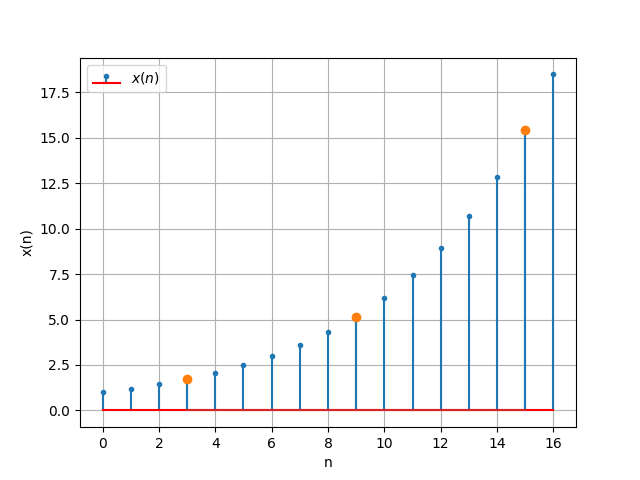
\includegraphics[width=\columnwidth]{ncert-maths/11/9/3/17/figs/A_1.png}
	\caption{Stem Plot of $x(n)$ vs $n$}
        \label{fig:1}
\end{figure}


\end{enumerate}


\pagebreak
\item Show that the ratio of the sum of the first \(n\) terms of a geometric progression (G.P.) to the sum of terms from \((n+1)\)th to \((2n)\)th term is \(\frac{1}{r^n}\).
\solution
\pagebreak
\item A G.P consists of an even number of terms. If the sum of all terms is 5 times the sum of terms occupying odd places, then find its common ratio.\\
\solution
\documentclass[journal,12pt,twocolumn]{IEEEtran}
\usepackage{cite}
\usepackage{amsmath,amssymb,amsfonts,amsthm}
\usepackage{algorithmic}
\usepackage{graphicx}
\usepackage{textcomp}
\usepackage{xcolor}
\usepackage{txfonts}
\usepackage{listings}
\usepackage{enumitem}
\usepackage{mathtools}
\usepackage{gensymb}
\usepackage{comment}
\usepackage[breaklinks=true]{hyperref}
\usepackage{tkz-euclide}
\usepackage{gvv}
\def\inputGnumericTable{}
\usepackage[latin1]{inputenc}
\usepackage{color}
\usepackage{array}
\usepackage{longtable}
\usepackage{calc}
\usepackage{multirow}
\usepackage{hhline}
\usepackage{ifthen}
\usepackage{lscape}

\newtheorem{theorem}{Theorem}[section]
\newtheorem{problem}{Problem}
\newtheorem{proposition}{Proposition}[section]
\newtheorem{lemma}{Lemma}[section]
\newtheorem{corollary}[theorem]{Corollary}
\newtheorem{example}{Example}[section]
\newtheorem{definition}[problem]{Definition}
\newcommand{\BEQA}{\begin{eqnarray}}
\newcommand{\EEQA}{\end{eqnarray}}
\newcommand{\define}{\stackrel{\triangle}{=}}
\theoremstyle{remark}
\newtheorem{rem}{Remark}
\begin{document}

\bibliographystyle{IEEEtran}
\title{Maths Assignment}
\author{Abhignya Gogula\\
        EE23BTECH11023}
\maketitle
\section*{Problem Statement}
A G.P consists of an even number of terms. If the sum of all terms is 5 times the sum of terms occupying odd places, then find its common ratio.
\section*{Solution}
\begin{table}[h!]
\centering
\begin{table}[h]
\renewcommand\thetable{1}
    \centering
    \begin{tabular}{|c|c|c|}
        \hline
        \textbf{Parameter} & \textbf{Description} & \textbf{Value}\\
        \hline
        $x(0)$ & First term & $2$\\
        \hline
        $x(19)$ & $20\textsuperscript{th}$ term & $-112$\\
        \hline
        $y(n)$ & sum upto $n\textsuperscript{th}$ term & \\
        \hline
    \end{tabular}
    \caption{Input data}
  \label{input data}
\end{table}

\caption{Input Parameters}
\label{11.9.5.11tab1}
\end{table}
Solving the Question in time domain:
\begin{align}
x(n) &= x(0)r^{n} \\
y(n) &= x(0)\brak{\frac{r^{n+1}-1}{r-1}}u(n)
\label{eq:11.9.5.11eq1}
\end{align}
The sum of terms in odd places:
\begin{align}
x_o(n) &= x(0)r^{2n}
\end{align}
\begin{equation}
y_o(n)= x(0)\brak{\frac{r^{n+1}-1}{r^2-1}}u(n)
\label{eq:11.9.5.11eq2}
\end{equation}
Then from \eqref{eq:11.9.5.11eq1} and \eqref{eq:11.9.5.11eq2}
\begin{align}
x(0)\brak{\frac{r^{N}-1}{r-1}}u(n) &= 5\brak{x(0)\brak{\frac{r^{2M}-1}{r^2-1}}u(n)}\\
\frac{r^2-1}{r-1} &= 5\\
\text{as } r \neq 1, \quad \text{hence } r &= 4\\
\end{align}
X,Y,Xo,Yo are frequency counterparts of the above GP
\begin{align}
X(z) &= \frac{x(0)}{1-rz^{-1}} \quad \abs{z} > \abs{r}\\ 
X_o(z) &= \frac{x(0)}{1-r^{2}z^{-1}}\\
Y(z) &= \frac{x(0)}{\brak{1-rz^{-1}}\brak{1-z^{-1}}}\\
Y_o(z) &= \frac{x(0)}{\brak{1-rz^{\frac{-1}{2}}}\brak{1-z^{-1}}}
\end{align}
\end{document}


\pagebreak
\item Find the sum to indicated number of terms in the geometric progression $x^3,x^5,x^7,...n$ terms (if $x\neq\pm1$).\\
\solution
\iffalse
\let\negmedspace\undefined
\let\negthickspace\undefined
\documentclass[journal,12pt,twocolumn]{IEEEtran}
\usepackage{cite}
\usepackage{amsmath,amssymb,amsfonts,amsthm}
\usepackage{algorithmic}
\usepackage{graphicx}
\usepackage{textcomp}
\usepackage{xcolor}
\usepackage{txfonts}
\usepackage{listings}
\usepackage{enumitem}
\usepackage{mathtools}
\usepackage{gensymb}
\usepackage{comment}
\usepackage[breaklinks=true]{hyperref}
\usepackage{tkz-euclide} 
\usepackage{listings}
\usepackage{gvv}                                        
\def\inputGnumericTable{}                                 
\usepackage[latin1]{inputenc}                                
\usepackage{color}                                            
\usepackage{array}                                            
\usepackage{longtable}                                       
\usepackage{calc}                                             
\usepackage{multirow}                                         
\usepackage{hhline}                                           
\usepackage{ifthen}                                           
\usepackage{lscape}
\newtheorem{theorem}{Theorem}[section]
\newtheorem{problem}{Problem}
\newtheorem{proposition}{Proposition}[section]
\newtheorem{lemma}{Lemma}[section]
\newtheorem{corollary}[theorem]{Corollary}
\newtheorem{example}{Example}[section]
\newtheorem{definition}[problem]{Definition}
\newcommand{\BEQA}{\begin{eqnarray}}
\newcommand{\EEQA}{\end{eqnarray}}
\newcommand{\define}{\stackrel{\triangle}{=}}
\theoremstyle{remark}
\newtheorem{rem}{Remark}
\begin{document}

\bibliographystyle{IEEEtran}
\vspace{3cm}

\title{NCERT 11.9.3.Q10}
\author{EE23BTECH11224 - Sri Krishna Prabhas Yadla$^{*}$% <-this % stops a space
}
\maketitle
\newpage
\bigskip

\renewcommand{\thefigure}{\arabic{figure}}
\renewcommand{\thetable}{\arabic{table}}


\vspace{3cm}
\textbf{Question:} Find the sum to indicated number of terms in the geometric progression $x^3,x^5,x^7,...n$ terms (if $x\neq\pm1$).
\\
\solution
\fi
\begin{table}[htbp]
\centering
\def\arraystrech{1.5}
	\begin{tabular}{|c|c|c|}
\hline
		\textbf{Input Parameters} & \textbf{Values} & \textbf{Description} \\
\hline
		$x(0)$ & $x^3$ & Initial term\\
\hline
		$r$ & $x^2$ & Common ratio\\
\hline
		$x(n)$ & $x^{2n+3}u(n)$ & General term \\
\hline
\end{tabular}
\caption{Given inputs}
\label{tab:1.11.9.3.Q10}
\end{table}

\newline
From \tabref{tab:1.11.9.3.Q10},
\begin{align}
	X(z) &= \frac{x(0)}{1-rz^{-1}} \\
	&= \frac{x^3}{1-x^2z^{-1}} \quad \abs{z}>x^2 \\
	y(n) &= x(n) * u(n) \\
	Y(z) &= X(z)U(z) \\
	&= \frac{x^3}{(1-x^2z^{-1})(1-z^{-1})} \quad  \abs{z} > x^2 \cap \abs{z}>1\\
	&= \frac{x^3}{x^2-1}\brak{\frac{x^2}{1-x^2z^{-1}}-\frac{1}{1-z^{-1}}} \\
	u(n) &\system{Z} \frac{1}{1-z^{-1}} \quad \abs{z}>1 \\
	x^{2n+2} u(n) &\system{Z} \frac{x^2}{1-x^2z^{-1}} \quad \abs{z}>x^2
\end{align}
Taking inverse Z transform of $Y(z)$,
\begin{align}
	y(n) &= x^3\brak{\frac{x^{2n+2}-1}{x^2-1}}u(n)
\end{align}
\begin{figure}[ht!]
	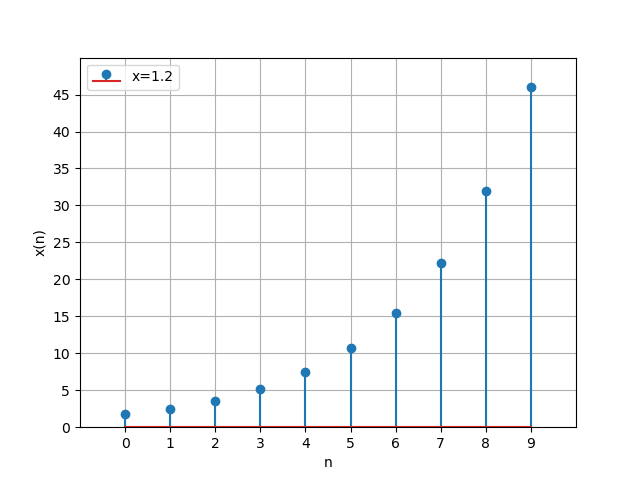
\includegraphics[width=\columnwidth]{ncert-maths/11/9/3/10/figs/plot_2.png}
	\caption{Plot of $x(n)$ for $x=1.2$}
	\label{fig:1.2}
\end{figure}

\pagebreak
\item Determine the AP whose third term is 16 and the 7th term exceeds the 5th term by 12. \\
\solution
\documentclass[12pt]{article}
\usepackage{amsmath}
\usepackage{graphicx}
\usepackage{float}
\usepackage{amssymb}
\usepackage{pgfplots}
\pgfplotsset{compat=1.18}
\newcommand{\tabref}[1]{Table~\ref{#1}}
\newcommand{\figref}[1]{Figure~\ref{#1}}
\providecommand{\abs}[1]{\left\vert#1\right\vert}

\begin{document}

\title{Discrete Assignment}
\author{Mohana Eppala\\ EE23BTECH11018}
\maketitle

\section*{Problem Statement}
Determine the AP whose third term is 16 and the 7th term exceeds the 5th term by 12. 
\section*{Solution}
\begin{table}[H]

\centering
\begin{tabular}{|c|c|c|}
        \hline
        \textbf{Parameter} & \textbf{Value} & \textbf{Description} \\
        \hline
        $x(6) - x(4)$ & 12 & 7th term exceeds 5th by 12 \\
        \hline
	$x(2)$ & 16 & Third term \\
	\hline
        $d$ & ? & Common difference \\
        \hline
        $x(0)$ & ? & First term of AP \\
	\hline
        $x(n)$ & $(x(0) + nd)u(n)$ & General term \\
        \hline
\end{tabular}
\caption{Input parameters table}
\label{tab:1}

\end{table}


From \tabref{tab:1}
\begin{align}
    x(0) +6d - x(0) - 4d &= 12 \\ \implies
    2d &= 12\\ \implies
    d &= 6
\end{align}
Also,
\begin{align}
     x(0) + 2d &= 16 \\ \implies
	x(0) + 2(6) &= 16 \\ \implies
	x(0) &= 4 \\
	\therefore x(n) &= 6n + 4 
\end{align}
From \tabref{tab:1}
\begin{align}
	X(z) &= x(0)  \frac{1}{1-z^{-1}} + d \frac{z^{-1}}{(1 - z^{-1})^2} \\
	&= 4 \frac{1}{1-z^{-1}} + 6 \frac{z^{-1}}{(1 - z^{-1})^2} \\
	&= \frac{4+2z^{-1}}{(1-z^{-1})^2} \quad \abs{z} > 1
\end{align}



\begin{figure}[H]
    \centering
    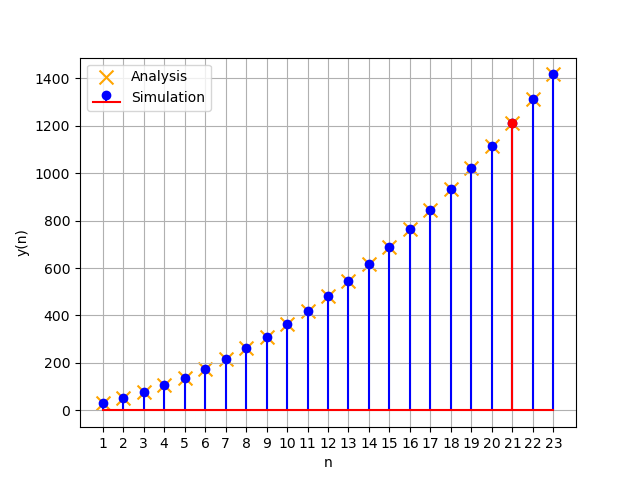
\includegraphics{figs/fig1.png}
    \caption{Given AP}
    \label{fig}
\end{figure}

\end{document}


\pagebreak
\item Find the seventh term of the sequence where the nth term is given by $a_n= \frac {n^2}{2^{n}}$\\
\solution

\iffalse
\documentclass[journal,12pt,twocolumn]{IEEEtran}
\usepackage{cite}
\usepackage{amsmath,amssymb,amsfonts,amsthm}
\usepackage{algorithmic}
\usepackage{graphicx}
\usepackage{textcomp}
\usepackage{xcolor}
\usepackage{txfonts}
\usepackage{listings}
\usepackage{enumitem}
\usepackage{mathtools}
\usepackage{float}
\usepackage{gensymb}
\usepackage{comment}
\usepackage[breaklinks=true]{hyperref}
\usepackage{tkz-euclide} 
\usepackage{listings}
\usepackage{gvv}                                        
\def\inputGnumericTable{}                                 
\usepackage[latin1]{inputenc}                                
\usepackage{color}                                            
\usepackage{array}                                            
\usepackage{longtable}                                       
\usepackage{calc}                                             
\usepackage{multirow}                                         
\usepackage{hhline}                                           
\usepackage{ifthen}                                           
\usepackage{lscape}
\usepackage{amsmath}
\newtheorem{theorem}{Theorem}[section]
\newtheorem{problem}{Problem}
\newtheorem{proposition}{Proposition}[section]
\newtheorem{lemma}{Lemma}[section]
\newtheorem{corollary}[theorem]{Corollary}
\newtheorem{example}{Example}[section]
\newtheorem{definition}[problem]{Definition}
\newcommand{\BEQA}{\begin{eqnarray}}
\newcommand{\EEQA}{\end{eqnarray}}
\newcommand{\define}{\stackrel{\triangle}{=}}
\theoremstyle{remark}
\newtheorem{rem}{Remark}

\begin{document}

\bibliographystyle{IEEEtran}
\vspace{3cm}

\title{NCERT Discrete - 11.9.1.8}
\author{EE23BTECH11045 - Palavelli Srija$^{*}$}

\maketitle
\newpage
\bigskip

\renewcommand{\thefigure}{\theenumi}
\renewcommand{\thetable}{\theenumi}

\vspace{3cm}
\textbf{Question 11.9.1.8:} 
\begin{enumerate}
\item Find the seventh term of the sequence where the nth term is given by $a_n= \frac {n^2}{2^{n}}$
\end{enumerate}

\textbf{Solution: }
\fi
\begin{align}
 x(n) &= \frac{(n+1)^2}{2^{(n+1)}}u(n)
\end{align}

\begin{table}[h!]
    \centering
     \begin{tabular}{|c|c|}
        \hline
        \textbf{Parameter} & \textbf{Value} \\
        \hline
        \(x(n)\) & \(\frac{(n+1)^2}{2^(n+1)}u(n)\) \\ \\
        \(x(6)\) & ? \\
        \hline
    \end{tabular}

    \caption{Input Parameters}
    \label{tab:table_sr}
\end{table}

\begin{align}
x(6) &= \frac{(6+1)^2}{2^{(6+1)}}\\
     &= \frac {49}{128}
\end{align}

\begin{enumerate}
   \item Scaling property:
     \begin{align}
         a^{n} u(n) & \xleftrightarrow{\mathcal{Z}}  \frac{1}{(1-az^{-1})}, \quad \lvert z \rvert > \lvert a \rvert 
     \end{align}
     
   \item Differentiation property:
    \begin{align}
     n u(n) & \xleftrightarrow{\mathcal{Z}} (-z) \frac{dY(z)}{dz} \\
     \implies n u(n) & \xleftrightarrow{\mathcal{Z}}  \frac{z^{-1}}{(1-z^{-1})^2}, \quad \lvert z \rvert > 1 \\
     \implies n^2 u(n) & \xleftrightarrow{\mathcal{Z}}  \frac{z^{-1}(1+z^{-1})}{(1-z^{-1})^3}, \quad \lvert z \rvert > 1
   \end{align}
   
   \item Time shifting property:
    \begin{align}
         y(n-k) & \xleftrightarrow{\mathcal{Z}} z^{-k}Y(z)
     \end{align}
\end{enumerate}

The Z transform of $x(n)$ is given by:\\
from(4)
\begin{align}
\frac{u(n)}{2^n} & \xleftrightarrow{\mathcal{Z}}  \frac{1}{(1-(2z)^{-1})}, \quad \lvert z \rvert>\frac{1}{2}
\end{align}
	from(5)
\begin{align}
\frac{n}{2^n} u(n) & \xleftrightarrow{\mathcal{Z}} \frac{(2z)^{-1}}{(1-(2z)^{-1})^2}, \quad \lvert z \rvert>\frac{1}{2}\\
\frac{n^2}{2^n} u(n) & \xleftrightarrow{\mathcal{Z}} \frac{(2z)^{-1}(1 + (2z)^{-1})}{(1 - (2z)^{-1})^3}, \quad \lvert z \rvert>\frac{1}{2}
\end{align}
	from(8)
\begin{align}
\frac{(n+1)^2}{2^(n+1)} u(n) & \xleftrightarrow{\mathcal{Z}} (z) \frac{(2z)^{-1}(1 + (2z)^{-1})}{(1 - (2z)^{-1})^3}, \quad \lvert z \rvert > \frac{1}{2}
\end{align}

\begin{align}
X(z) &= \frac{1 + (2z)^{-1}}{2(1 - (2z)^{-1})^3}, \quad \lvert z \rvert > \frac{1}{2}
\end{align}

\begin{figure}[h!]
    \centering
    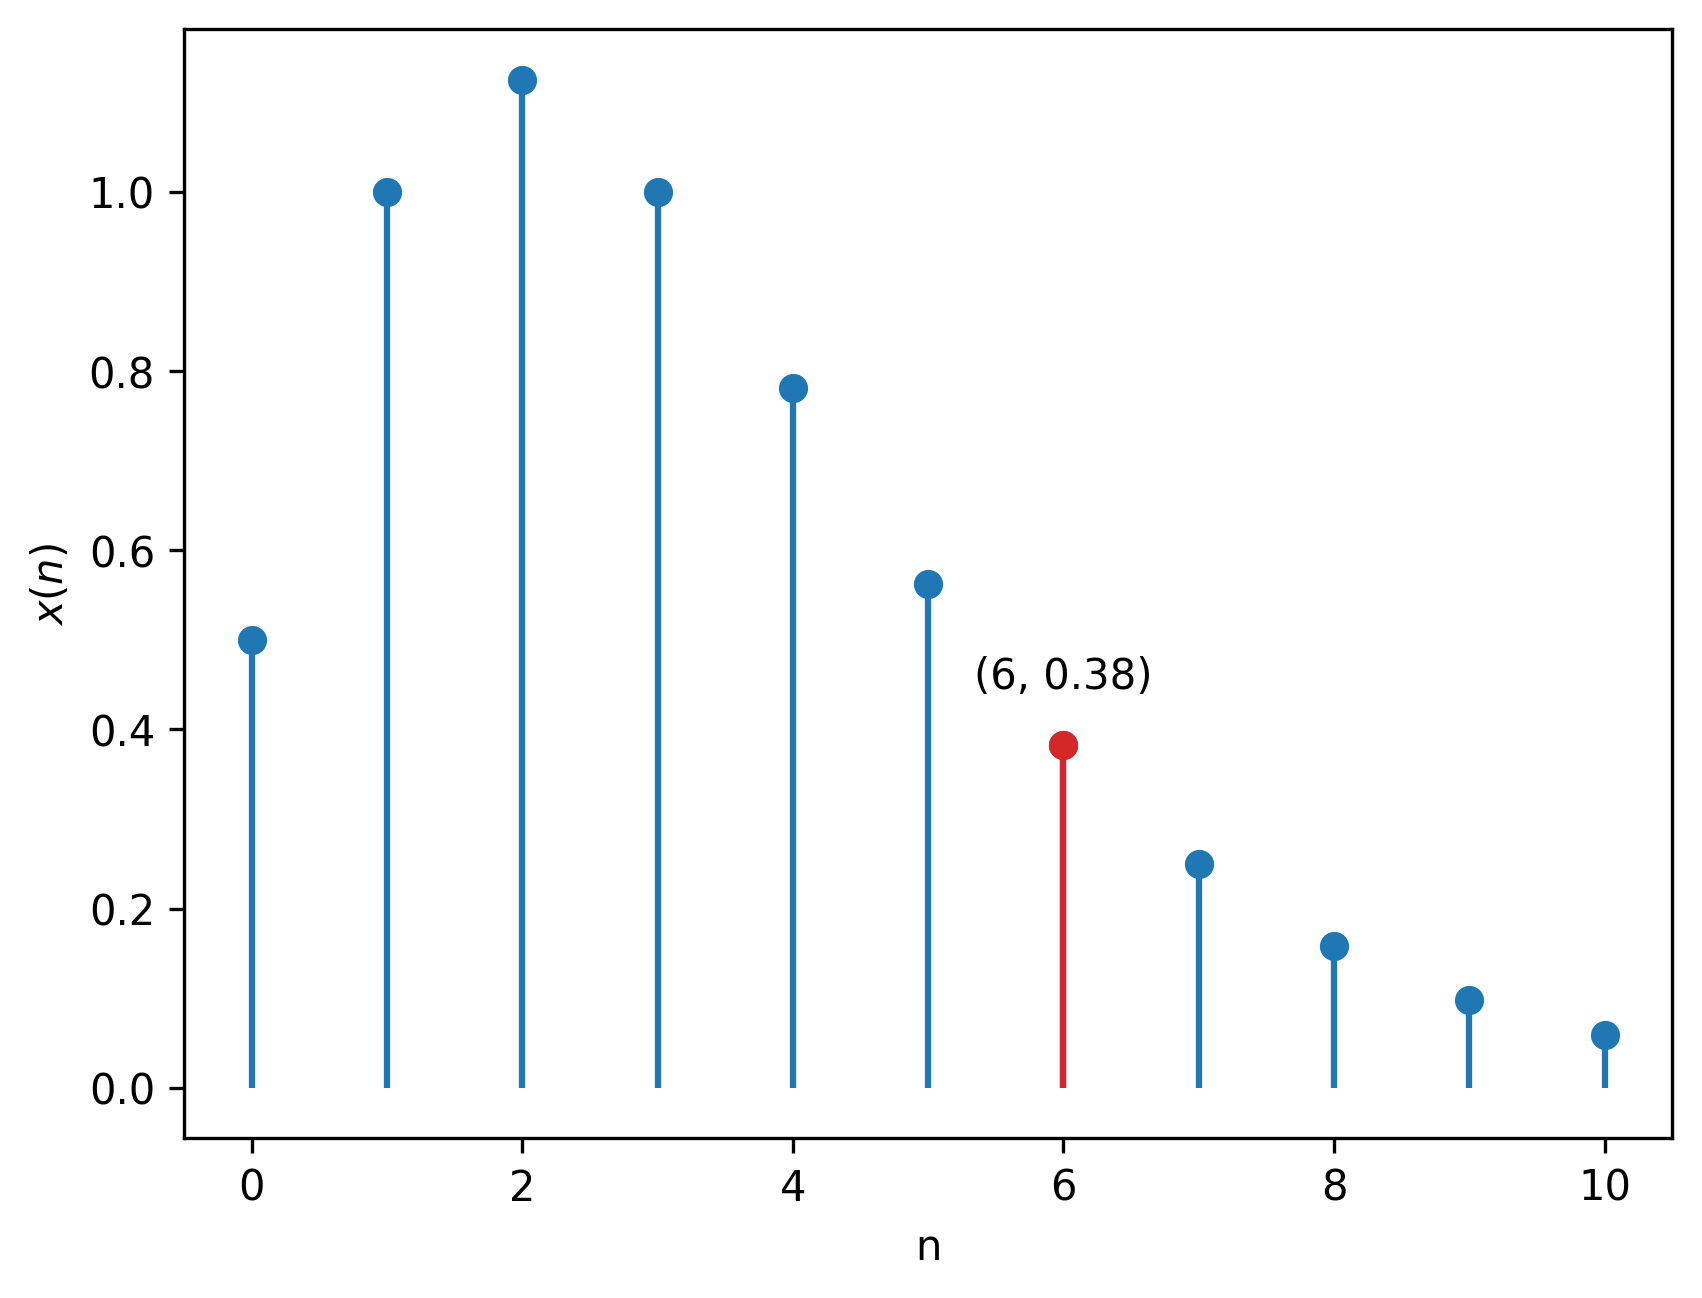
\includegraphics[width=\columnwidth]{ncert-maths/11/9/1/8/figs/plot.png}
    \caption{Stem plot of $x(n)$}
    \label{fig:sr1}
\end{figure}

%\end{document}

\pagebreak
\item Find sum to n terms of the following series:\\
$\frac{1}{1 \times 2} + \frac{1}{2 \times 3} + \frac{1}{3 \times 4} + \ldots$ \hfill(NCERT 11.9.4.4)
\solution
\pagebreak
\item 1x2x3 + 2x3x4 + 3x4x5 +..... \\
\solution
\pagebreak
\item  Find the sum of the following series up to \(n\) terms:
          \begin{enumerate}
              \item $5 + 55 + 555 + \ldots$
              \item  $.6 + .66 + .666 + \ldots$
        \end{enumerate}

\solution
\pagebreak
\item Find $a_{9}$ in the sequence $a_{n}=\brak{-1}^{n-1}n^{3}$ \\
\solution
\pagebreak
\item Find the 20th term in this series.\\
$$2\times4+4\times6+6\times8\cdots+n\,terms$$ \\
\solution
\pagebreak

\item Q10) The sum of three numbers in G.P. is 56. If we subtract 1, 7, 21 from these numbers in that order, we obtain an arithmetic progression. Find the numbers.\\
\solution
\item  Find the sum to n terms for the given series: $3\times8 + 6\times11 + 9\times14 + ...$
\solution
\pagebreak
\item Find a GP for which sum of the first two terms is -4 and the fifth term is 4 times the third term.\\
\solution
\iffalse
\let\negmedspace\undefined
\let\negthickspace\undefined
\documentclass[journal,12pt,twocolumn]{IEEEtran}
\usepackage{cite}
\usepackage{amsmath,amssymb,amsfonts,amsthm}
\usepackage{algorithmic}
\usepackage{graphicx}
\usepackage{textcomp}
\usepackage{xcolor}
\usepackage{txfonts}
\usepackage{listings}
\usepackage{enumitem}
\usepackage{mathtools}
\usepackage{gensymb}
\usepackage{comment}
\usepackage[breaklinks=true]{hyperref}
\usepackage{tkz-euclide} % loads  TikZ and tkz-base
\usepackage{listings}
\usepackage[latin1]{inputenc}                                
\usepackage{color}                                            
\usepackage{array}                                            
\usepackage{longtable}                                       
\usepackage{calc}                                             
\usepackage{multirow}                                         
\usepackage{hhline}                                           
\usepackage{ifthen}                                           
\usepackage{lscape}
\usepackage{caption}
\usepackage{subcaption}


\newtheorem{theorem}{Theorem}[section]
\newtheorem{problem}{Problem}
\newtheorem{proposition}{Proposition}[section]
\newtheorem{lemma}{Lemma}[section]
\newtheorem{corollary}[theorem]{Corollary}
\newtheorem{example}{Example}[section]
\newtheorem{definition}[problem]{Definition}
%\newtheorem{thm}{Theorem}[section] 
%\newtheorem{defn}[thm]{Definition}
%\newtheorem{algorithm}{Algorithm}[section]
%\newtheorem{cor}{Corollary}
\newcommand{\BEQA}{\begin{eqnarray}}
\newcommand{\EEQA}{\end{eqnarray}}
\newcommand{\define}{\stackrel{\triangle}{=}}
\theoremstyle{remark}
\newtheorem{rem}{Remark}
%\bibliographystyle{ieeetr}

\begin{document}

%
\providecommand{\pr}[1]{\ensuremath{\Pr\left(#1\right)}}
\providecommand{\prt}[2]{\ensuremath{p_{#1}^{\left(#2\right)} }}        % own macro for this question
\providecommand{\qfunc}[1]{\ensuremath{Q\left(#1\right)}}
\providecommand{\sbrak}[1]{\ensuremath{{}\left[#1\right]}}
\providecommand{\lsbrak}[1]{\ensuremath{{}\left[#1\right.}}
\providecommand{\rsbrak}[1]{\ensuremath{{}\left.#1\right]}}
\providecommand{\brak}[1]{\ensuremath{\left(#1\right)}}
\providecommand{\lbrak}[1]{\ensuremath{\left(#1\right.}}
\providecommand{\rbrak}[1]{\ensuremath{\left.#1\right)}}
\providecommand{\cbrak}[1]{\ensuremath{\left\{#1\right\}}}
\providecommand{\lcbrak}[1]{\ensuremath{\left\{#1\right.}}
\providecommand{\rcbrak}[1]{\ensuremath{\left.#1\right\}}}
\newcommand{\sgn}{\mathop{\mathrm{sgn}}}
\providecommand{\abs}[1]{\left\vert#1\right\vert}
\providecommand{\res}[1]{\Res\displaylimits_{#1}} 
\providecommand{\norm}[1]{\left\lVert#1\right\rVert}
%\providecommand{\norm}[1]{\lVert#1\rVert}
\providecommand{\mtx}[1]{\mathbf{#1}}
\providecommand{\mean}[1]{E\left[ #1 \right]}
\providecommand{\cond}[2]{#1\middle|#2}
\providecommand{\fourier}{\overset{\mathcal{F}}{ \rightleftharpoons}}
\newenvironment{amatrix}[1]{%
  \left(\begin{array}{@{}*{#1}{c}|c@{}}
}{%
  \end{array}\right)
}
%\providecommand{\hilbert}{\overset{\mathcal{H}}{ \rightleftharpoons}}
%\providecommand{\system}{\overset{\mathcal{H}}{ \longleftrightarrow}}
        %\newcommand{\solution}[2]{\textbf{Solution:}{#1}}
\newcommand{\solution}{\noindent \textbf{Solution: }}
\newcommand{\cosec}{\,\text{cosec}\,}
\providecommand{\dec}[2]{\ensuremath{\overset{#1}{\underset{#2}{\gtrless}}}}
\newcommand{\myvec}[1]{\ensuremath{\begin{pmatrix}#1\end{pmatrix}}}
\newcommand{\mydet}[1]{\ensuremath{\begin{vmatrix}#1\end{vmatrix}}}
\newcommand{\myaugvec}[2]{\ensuremath{\begin{amatrix}{#1}#2\end{amatrix}}}
\providecommand{\rank}{\text{rank}}
\providecommand{\pr}[1]{\ensuremath{\Pr\left(#1\right)}}
\providecommand{\qfunc}[1]{\ensuremath{Q\left(#1\right)}}
        \newcommand*{\permcomb}[4][0mu]{{{}^{#3}\mkern#1#2_{#4}}}
\newcommand*{\perm}[1][-3mu]{\permcomb[#1]{P}}
\newcommand*{\comb}[1][-1mu]{\permcomb[#1]{C}}
\providecommand{\qfunc}[1]{\ensuremath{Q\left(#1\right)}}
\providecommand{\gauss}[2]{\mathcal{N}\ensuremath{\left(#1,#2\right)}}
\providecommand{\diff}[2]{\ensuremath{\frac{d{#1}}{d{#2}}}}
\providecommand{\myceil}[1]{\left \lceil #1 \right \rceil }
\newcommand\figref{Fig.~\ref}
\newcommand\tabref{Table~\ref}
\newcommand{\sinc}{\,\text{sinc}\,}
\newcommand{\rect}{\,\text{rect}\,}
%%
%       %\newcommand{\solution}[2]{\textbf{Solution:}{#1}}
%\newcommand{\solution}{\noindent \textbf{Solution: }}
%\newcommand{\cosec}{\,\text{cosec}\,}
%\numberwithin{equation}{section}
%\numberwithin{equation}{subsection}
%\numberwithin{problem}{section}
%\numberwithin{definition}{section}
%\makeatletter
%\@addtoreset{figure}{problem}
%\makeatother

%\let\StandardTheFigure\thefigure
\let\vec\mathbf

\bibliographystyle{IEEEtran}

\vspace{3cm}
\title{Assignment}
\author{EE23BTECH11001 - Aashna Sahu}
\maketitle
\bigskip

\renewcommand{\thefigure}{\theenumi}
\renewcommand{\thetable}{\theenumi}
%\renewcommand{\theequation}{\theenumi}
Q:Find a GP for which sum of the first two terms is -4 and the fifth term is 4 times the third term.

\solution
\fi

\begin{table}[ht]
  \centering
  \begin{tabular}{|c|c|c|}
      \hline
      Parameter & Description & Value\\\hline
      $x(0)$ & First term of AP & --\\\hline
      $r$ & Common ratio & --\\\hline
      $x(n)$ & General term of given AP & $x(0)r^nu(n)$\\\hline
      $x(0)+x(1)$ & sum of 1st and 2nd term & $-4$\\\hline
      $\displaystyle\frac{x(4)}{x(2)}$ & Ratio of 5th and 3rd term & $4$\\\hline
\end{tabular}

  \caption{Input Parameters}
  \label{tab:table1}
\end{table}
From \tabref{tab:table1}:
\begin{align}
x(0)r^4&=4x(0)r^2\\
\implies r&=\pm 2
\label{eq:eq2}
\end{align}

From \tabref{tab:table1} and \eqref{eq:eq2} :\\
\begin{align}
x(0)r+x(0)&=-4\\
\implies x(0)&=\frac{-4}{r+1}\\
x(0) &=
\begin{cases}
   \displaystyle\frac{-4}{3}  , & r=+2 \\
      4  , & r=-2 \\
\end{cases}\\
   X(z)&=\frac{x(0)}{1-rz^{-1}}\quad ,\abs{z}>\abs{r}\\
X(z) &=
\begin{cases}
   \displaystyle\frac{4}{3(2z^{-1}-1)}, & r=+2\\
   \displaystyle\frac{4}{1+2z^{-1}}, & r=-2\\
\end{cases}
\end{align}

\[\abs{z}>2\]

\begin{figure}[h]
  \centering
  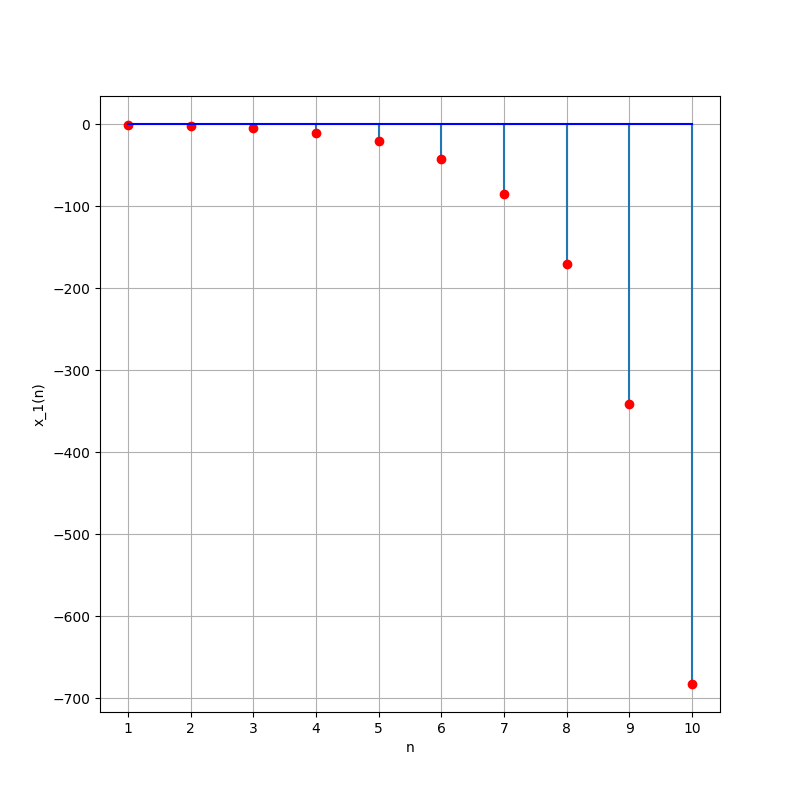
\includegraphics[width=1.0\columnwidth]{ncert-maths/11/9/3/16/figs/plot1.png}
  \caption{Representation of x(n) for $r=2$}
  \label{fig:fig1}
\end{figure}
\begin{figure}[h]
  \centering
  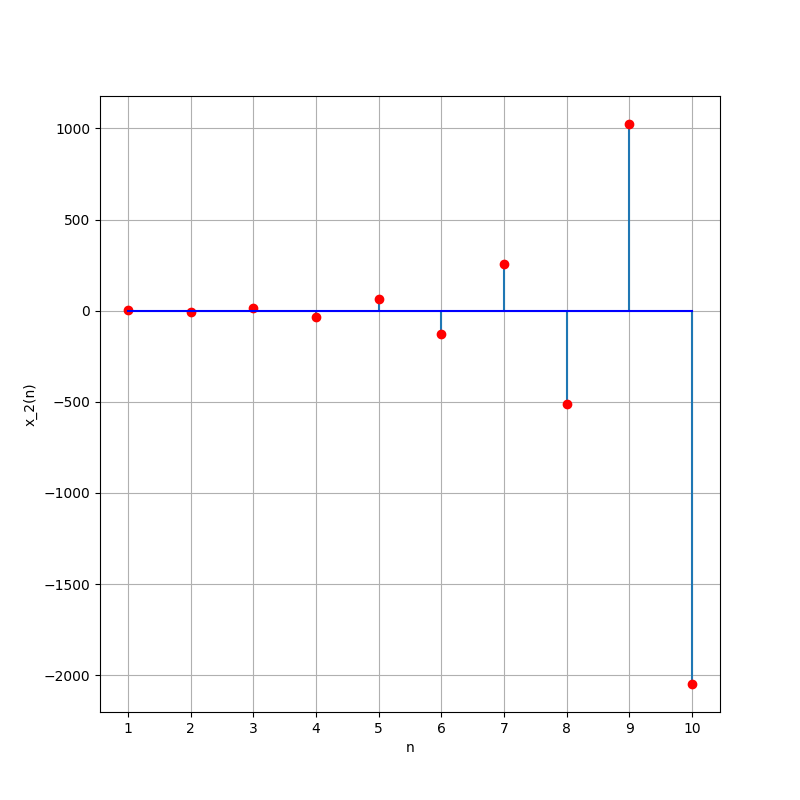
\includegraphics[width=1.0\columnwidth]{ncert-maths/11/9/3/16/figs/plot2.png}
  \caption{Representation of x(n) for $r=-2$}
  \label{fig:fig2}
\end{figure}


%\end{document}

\pagebreak
\end{enumerate}

\chapter{Sequences}
\begin{enumerate}[label=\thesection.\arabic*,ref=\thesection.\theenumi]
\item Find the number of terms in each of the following APs. 
\begin{enumerate}
    \item 7, 13, 19, ... 205

    \item 18, 15$\frac{1}{2}$, 13, ... -47
\end{enumerate}
\solution
\iffalse
\let\negmedspace\undefined
\let\negthickspace\undefined
\documentclass[journal,12pt,twocolumn]{IEEEtran}
\usepackage{cite}
\usepackage{amsmath,amssymb,amsfonts,amsthm}
\usepackage{algorithmic}
\usepackage{graphicx}
\usepackage{textcomp}
\usepackage{xcolor}
\usepackage{txfonts}
\usepackage{listings}
\usepackage{enumitem}
\usepackage{mathtools}
\usepackage{gensymb}
\usepackage{comment}
\usepackage[breaklinks=true]{hyperref}
\usepackage{tkz-euclide} 
\usepackage{listings}
\usepackage{gvv}                                        
\def\inputGnumericTable{}                                 
\usepackage[latin1]{inputenc}                                
\usepackage{color}                                            
\usepackage{array}                                            
\usepackage{longtable}                                       
\usepackage{calc}                                             
\usepackage{multirow}                                         
\usepackage{hhline}                                           
\usepackage{ifthen}                                           
\usepackage{lscape}
\usepackage{placeins}
\usepackage{xparse}


\newtheorem{theorem}{Theorem}[section]
\newtheorem{problem}{Problem}
\newtheorem{proposition}{Proposition}[section]
\newtheorem{lemma}{Lemma}[section]
\newtheorem{corollary}[theorem]{Corollary}
\newtheorem{example}{Example}[section]
\newtheorem{definition}[problem]{Definition}
\newcommand{\BEQA}{\begin{eqnarray}}
\newcommand{\EEQA}{\end{eqnarray}}
\newcommand{\define}{\stackrel{\triangle}{=}}
\theoremstyle{remark}
\newtheorem{rem}{Remark}



\begin{document}

\bibliographystyle{IEEEtran}
\vspace{3cm}

\Large\title{NCERT Question 10.5.2.5}
\large\author{EE23BTECH11032 - Kaustubh Parag Khachane $^{*}$% <-this % stops a space
}
\maketitle
\newpage
\bigskip

\renewcommand{\thefigure}{\theenumi}
\renewcommand{\thetable}{\theenumi}
\large\textbf{Question 10.5.2.5} : \normalsize Find the number of terms in each of the following APs. Then express each term as x\brak{n} and find the z transform, ROC and plot the graph for x\brak{n}: 
\begin{enumerate}
    \item 7, 13, 19, ... 205

    \item 18, 15$\frac{1}{2}$, 13, ... -47
\end{enumerate}


\solution
\fi
\begin{table}[ht] 
\centering
\setlength{\extrarowheight}{8pt}
\begin{tabular}{|c|l|l|} 
 \hline
  \textbf{Parameter} & \textbf{Used to denote } & \textbf{Values} \\ 
 \hline
 $x_{i}$\brak{n} & $n^{th}$ term of $i^{th}$ series $\brak{i =\brak{1,2}}$  & $\brak{x_{i}\brak{0} + nd_{i}}u\brak{n}$ \\
 \hline
$x_{i}$\brak{0} & First term of $i^{th} $ AP &\multicolumn{1}{|p{1.5cm}|}{\centering $x_{1}\brak{0} = 7$ \\ $x_{2}\brak{0} = 18$ }\\
 \hline
  $d_{i}$ & Commmon difference of $i^{th}$ AP&\multicolumn{1}{|p{1.5cm}|}{\centering $d_{1} = 6 $ \\ $d_{2} = -2.5$}\\
 \hline

\end{tabular}
 \vspace{4mm}
 \caption{Parameter Table}
 \label{tab:table0}
\end{table}

The number of terms in the AP x\brak{n} is given by: 
\begin{align}  \label{eq:eq12}
    \frac{x\brak{n} - x\brak{0}}{d} + 1
\end{align}
\begin{align}
    &X_i(z) = \frac{x_i\brak{0}}{1 - z^{-1}} + d_i\frac{z^{-1}}{\brak{1-z^{-1}}^2} \text{ , for i=1,2} \label{eq:eq3}\\
    &\text{ROC : $\abs{z} > 1$ as it is an AP}   
\end{align}
\begin{enumerate}
    \item 
\begin{align}
x_{1}\brak{n} &= \brak{7 + \brak{n}6}u\brak{n}
\end{align}
Using the values in \tabref{tab:table0} and equation \eqref{eq:eq12},
\begin{align}
    k_1 = \frac{205 - 7}{6} + 1 = 34
\end{align}

Using the values in \tabref{tab:table0} and equation \eqref{eq:eq3} :
\begin{align}
 X_1\brak{z} = \frac{7 - z^{-1}}{\brak{1-z^{-1}}^2}
\end{align}

ROC is $\abs{z} > 1$
 
   \item
   
\begin{align}
    x_{2}\brak{n} &= \brak{18 + n\brak{-2.5}u\brak{n}}
\end{align}

Using the values in \tabref{tab:table0} and equation \eqref{eq:eq12},
\begin{align}
    k_2 = \frac{-47 - 18}{-2.5} + 1 = 27
\end{align}

Using the values in \tabref{tab:table0} and equation \eqref{eq:eq3} :
\begin{align} 
 X_2\brak{z} = \frac{18 - \brak{20.5}z^{-1}}{\brak{1 - z^{-1}}^2}
\end{align}

ROC is $\abs{z} > 1$.

\begin{figure}[!ht]
\centering
\begin{center}
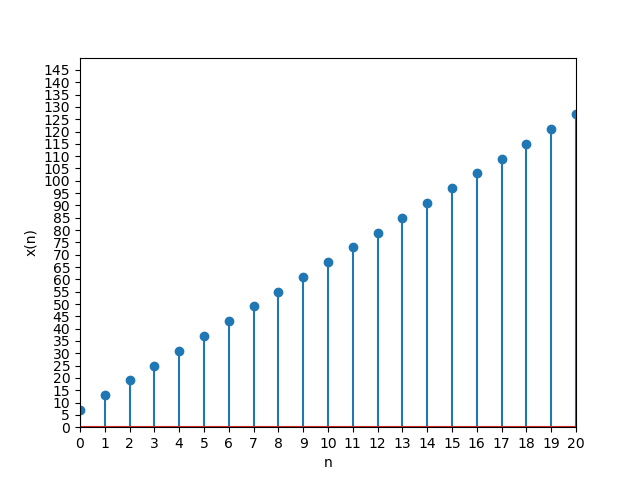
\includegraphics[width=\columnwidth]{ncert-maths/10/5/2/5/figs/Figure_1}
\caption{Plot of $x_1\brak{n}$}
\end{center}
\end{figure}

\begin{figure}[!ht]
\centering
\begin{center}
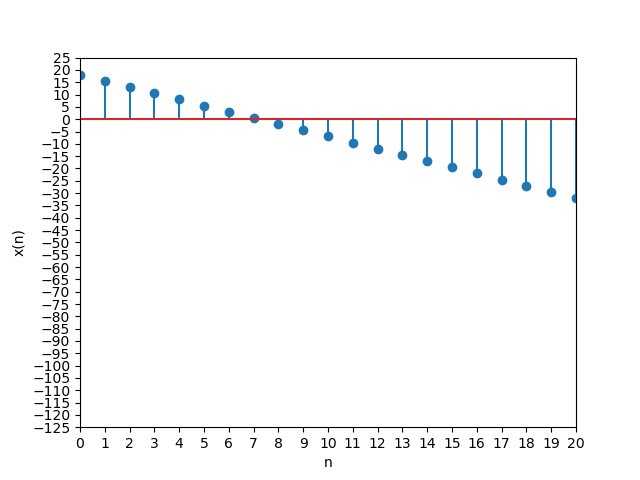
\includegraphics[width=\columnwidth]{ncert-maths/10/5/2/5/figs/Figure_2}
\caption{Plot of $x_2\brak{n}$}
\end{center}
\end{figure}

\end{enumerate}
%\end{document}



\item For what value of $ n$, are the $ nth$ terms of two A.Ps: 63, 65, 67,\dots and 3, 10, 17,\dots equal?
\solution
\iffalse
\let\negmedspace\undefined
\let\negthickspace\undefined
\documentclass[journal,12pt,twocolumn]{IEEEtran}
\usepackage{cite}
\usepackage{amsmath,amssymb,amsfonts,amsthm}
\usepackage{algorithmic}
\usepackage{graphicx}
\usepackage{textcomp}
\usepackage{xcolor}
\usepackage{txfonts}
\usepackage{listings}
\usepackage{enumitem}
\usepackage{mathtools}
\usepackage{gensymb}
\usepackage{comment}
\usepackage[breaklinks=true]{hyperref}
\usepackage{tkz-euclide}
\usepackage{listings}
\usepackage{gvv}
\def\inputGnumericTable{}
\usepackage[latin1]{inputenc}
\usepackage{color}
\usepackage{array}
\usepackage{longtable}
\usepackage{calc}
\usepackage{multirow}
\usepackage{hhline}
\usepackage{ifthen}
\usepackage{lscape}

\newtheorem{theorem}{Theorem}[section]
\newtheorem{problem}{Problem}
\newtheorem{proposition}{Proposition}[section]
\newtheorem{lemma}{Lemma}[section]
\newtheorem{corollary}[theorem]{Corollary}
\newtheorem{example}{Example}[section]
\newtheorem{definition}[problem]{Definition}
\newcommand{\BEQA}{\begin{eqnarray}}
\newcommand{\EEQA}{\end{eqnarray}}
\newcommand{\define}{\stackrel{\triangle}{=}}
\theoremstyle{remark}
\newtheorem{rem}{Remark}
\begin{document}

\bibliographystyle{IEEEtran}
\vspace{3cm}

\title{NCERT Discrete 10.5.2 -15}
\author{EE23BTECH11057 - Shakunaveti Sai Sri Ram Varun$^{}$% &lt;-this % stops a space
}
\maketitle
\newpage
\bigskip

\vspace{2cm}
\textbf{Question: }
For what value of $ n$, are the $ nth$ terms of two A.Ps: 63, 65, 67,\dots and 3, 10, 17,\dots equal?\\
\vspace{0.5cm}
\textbf{Solution}:
\fi

\begin{table}[htbp] 
\centering
\begin{tabular}{|c|c|c|c|}
    \hline
    \textbf{Parameter} & \textbf{Sub-question} & \textbf{Description} & \textbf{Value} \\
    \hline
    \multirow{2}{*}{$x_i\brak{0}$} & $x_1\brak{0}$ & $1^{st}$ term of $1^{st}$ A.P. & 63 \\
    \cline{2-4}
    & $x_2\brak{0}$ & $1^{st}$ term of $2^{nd}$ A.P. & \phantom{0}3 \\
    \hline
    \multirow{2}{*}{$d_i$} & $d_1$ & Common difference of $1^{st}$ A.P. & \phantom{0}2 \\
    \cline{2-4}
    & $d_2$ & Common difference of $2^{nd}$ A.P. & \phantom{0}7 \\
    \hline
\end{tabular}

\caption{input values}
\label{tab: table10.5.2.15}
\end{table}
\begin{align}
x_i\brak{n} &= x\brak{0}u\brak{n} + dnu\brak{n}\\
X\brak{z} &= \frac{x\brak{0}}{1-z^{-1}} + \frac{dz^{-1}}{\brak{1-z^{-1}}^{2}} \quad |z|>1
\end{align}
\begin{enumerate}
\item
\begin{align}
x_1\brak{n} &= 63u\brak{n} + 2nu\brak{n} \\
%To find $ X_1\brak{z}$:
X_1\brak{z} &= \frac{63}{1-z^{-1}} + \frac{2z^{-1}}{\brak{1-z^{-1}}^{2}}  \quad |z|>1
\end{align}
\item
\begin{align}
x_2\brak{n} &= 3u\brak{n} + 7nu\brak{n}\\ 
%To find $ X_2\brak{z}$ :\\
X_2\brak{z} &= \frac{3}{1-z^{-1}} + \frac{7z^{-1}}{\brak{1-z^{-1}}^{2}} \quad |z|>1
\end{align}
\item

given,
\begin{align}
 x_1\brak{n} &= x_2\brak{n}\\
\therefore 63 + 2n &= 7n+3\\
\implies n &=12
\end{align}
\begin{figure}[h!]
    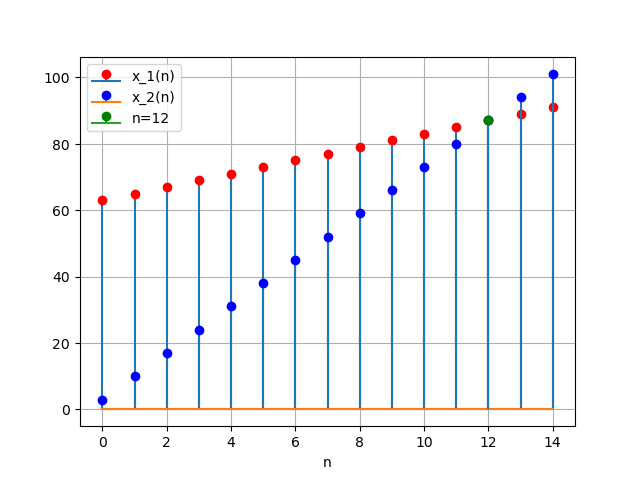
\includegraphics[width = \columnwidth]{ncert-maths/10/5/2/15/figs/Figure_1.png}
    \caption{Graphs of $ x_1\brak{n}$ and $ x_2\brak{n}$ and both are equal at $ n=12$}
    \label{fig: fig10.5.2.15}
\end{figure}
\end{enumerate}



\item Two APs have the same common difference.The difference between their $100${th} terms is 100,what is the difference between their $1000${th} terms?

\solution
\let\negmedspace\undefined
\let\negthickspace\undefined
\documentclass[journal,12pt,onecolumn]{IEEEtran}
\usepackage{cite}
\usepackage{amsmath,amssymb,amsfonts,amsthm}
\usepackage{algorithmic}
\usepackage{graphicx}
\usepackage{textcomp}
\usepackage{xcolor}
\usepackage{txfonts}
\usepackage{listings}
\usepackage{enumitem}
\usepackage{mathtools}
\usepackage{gensymb}
\usepackage[breaklinks=true]{hyperref}
\usepackage{tkz-euclide} % loads  TikZ and tkz-base
\usepackage{listings}



\newtheorem{theorem}{Theorem}[section]
\newtheorem{problem}{Problem}
\newtheorem{proposition}{Proposition}[section]
\newtheorem{lemma}{Lemma}[section]
\newtheorem{corollary}[theorem]{Corollary}
\newtheorem{example}{Example}[section]
\newtheorem{definition}[problem]{Definition}
%\newtheorem{thm}{Theorem}[section] 
%\newtheorem{defn}[thm]{Definition}
%\newtheorem{algorithm}{Algorithm}[section]
%\newtheorem{cor}{Corollary}
\newcommand{\BEQA}{\begin{eqnarray}}
\newcommand{\EEQA}{\end{eqnarray}}
\newcommand{\define}{\stackrel{\triangle}{=}}
\theoremstyle{remark}
\newtheorem{rem}{Remark}
%\bibliographystyle{ieeetr}
\begin{document}
%
\providecommand{\pr}[1]{\ensuremath{\Pr\left(#1\right)}}
\providecommand{\prt}[2]{\ensuremath{p_{#1}^{\left(#2\right)} }}        % own macro for this question
\providecommand{\qfunc}[1]{\ensuremath{Q\left(#1\right)}}
\providecommand{\sbrak}[1]{\ensuremath{{}\left[#1\right]}}
\providecommand{\lsbrak}[1]{\ensuremath{{}\left[#1\right.}}
\providecommand{\rsbrak}[1]{\ensuremath{{}\left.#1\right]}}
\providecommand{\brak}[1]{\ensuremath{\left(#1\right)}}
\providecommand{\lbrak}[1]{\ensuremath{\left(#1\right.}}
\providecommand{\rbrak}[1]{\ensuremath{\left.#1\right)}}
\providecommand{\cbrak}[1]{\ensuremath{\left\{#1\right\}}}
\providecommand{\lcbrak}[1]{\ensuremath{\left\{#1\right.}}
\providecommand{\rcbrak}[1]{\ensuremath{\left.#1\right\}}}
\newcommand{\sgn}{\mathop{\mathrm{sgn}}}
\providecommand{\abs}[1]{\left\vert#1\right\vert}
\providecommand{\res}[1]{\Res\displaylimits_{#1}} 
\providecommand{\norm}[1]{\left\lVert#1\right\rVert}
%\providecommand{\norm}[1]{\lVert#1\rVert}
\providecommand{\mtx}[1]{\mathbf{#1}}
\providecommand{\mean}[1]{E\left[ #1 \right]}
\providecommand{\cond}[2]{#1\middle|#2}
\providecommand{\fourier}{\overset{\mathcal{F}}{ \rightleftharpoons}}
\newenvironment{amatrix}[1]{%
  \left(\begin{array}{@{}*{#1}{c}|c@{}}
}{%
  \end{array}\right)
}
%\providecommand{\hilbert}{\overset{\mathcal{H}}{ \rightleftharpoons}}
%\providecommand{\system}{\overset{\mathcal{H}}{ \longleftrightarrow}}
	%\newcommand{\solution}[2]{\textbf{Solution:}{#1}}
\newcommand{\solution}{\noindent \textbf{Solution: }}
\newcommand{\cosec}{\,\text{cosec}\,}
\providecommand{\dec}[2]{\ensuremath{\overset{#1}{\underset{#2}{\gtrless}}}}
\newcommand{\myvec}[1]{\ensuremath{\begin{pmatrix}#1\end{pmatrix}}}
\newcommand{\mydet}[1]{\ensuremath{\begin{vmatrix}#1\end{vmatrix}}}
\newcommand{\myaugvec}[2]{\ensuremath{\begin{amatrix}{#1}#2\end{amatrix}}}
\providecommand{\rank}{\text{rank}}
\providecommand{\pr}[1]{\ensuremath{\Pr\left(#1\right)}}
\providecommand{\qfunc}[1]{\ensuremath{Q\left(#1\right)}}
	\newcommand*{\permcomb}[4][0mu]{{{}^{#3}\mkern#1#2_{#4}}}
\newcommand*{\perm}[1][-3mu]{\permcomb[#1]{P}}
\newcommand*{\comb}[1][-1mu]{\permcomb[#1]{C}}
\providecommand{\qfunc}[1]{\ensuremath{Q\left(#1\right)}}
\providecommand{\gauss}[2]{\mathcal{N}\ensuremath{\left(#1,#2\right)}}
\providecommand{\diff}[2]{\ensuremath{\frac{d{#1}}{d{#2}}}}
\providecommand{\myceil}[1]{\left \lceil #1 \right \rceil }
\newcommand\figref{Fig.~\ref}
\newcommand\tabref{Table~\ref}
\newcommand{\sinc}{\,\text{sinc}\,}
\newcommand{\rect}{\,\text{rect}\,}
%%
%	%\newcommand{\solution}[2]{\textbf{Solution:}{#1}}
%\newcommand{\solution}{\noindent \textbf{Solution: }}
%\newcommand{\cosec}{\,\text{cosec}\,}
%\numberwithin{equation}{section}
%\numberwithin{equation}{subsection}
%\numberwithin{problem}{section}
%\numberwithin{definition}{section}
%\makeatletter
%\@addtoreset{figure}{problem}
%\makeatother

%\let\StandardTheFigure\thefigure
\let\vec\mathbf


\bibliographystyle{IEEEtran}
\title{SEQUENCES}
\author{EE23BTECH11011- Batchu Ishitha$^{*}$% <-this % stops a space
}
\maketitle




\bigskip

\renewcommand{\thefigure}{\theenumi}
\renewcommand{\thetable}{\theenumi}
%\renewcommand{\theequation}{\theenumi}

Q:Two APs have the same common difference.The difference between their $100${th} terms is 100,what is the difference between their $1000${th} terms?

\solution

\begin{align}
x(n) &= \{x(0)+nd\}u(n) \\
 x(99) - y(99) &= 100 \\
\implies (x(0) + 99d) - (y(0) + 99d) &= 100
 \\
\implies x(0) - y(0) &= 100
\end{align}

\begin{align}
x(n) - y(n) &= (x(0) + nd) - (y(0) + nd)\\
&= x(0) - y(0) \\
&= 100 \\
\implies x(999)-y(999)&=100 
\end{align}

\begin{table}[!ht]
    \centering
        \begin{table}[ht]
    \centering
    \begin{tabular}{|c|c|c|}
        \hline
        Parameter & Value & Description \\
        \hline
        $x(0)$ & 5 & First term of AP \\
        $d$ & 1.75 & Common difference of AP \\
        $x(n)$ & 20.75 & $n^{th}$ term of AP \\
        \hline
    \end{tabular}
    \vspace{2mm}
    \caption{Parameter List}
    \label{tab:simple.10.5.2.20}
\end{table}

    \caption{input parameters}
    \label{tab:10_5_3_12}
\end{table}
Let 
\begin{align}
x(n)&= \lbrace 101,106,111,...\rbrace \\
y(n)&= \lbrace 1,6,11,... \rbrace
\end{align}


\begin{figure}[h]
    \centering
    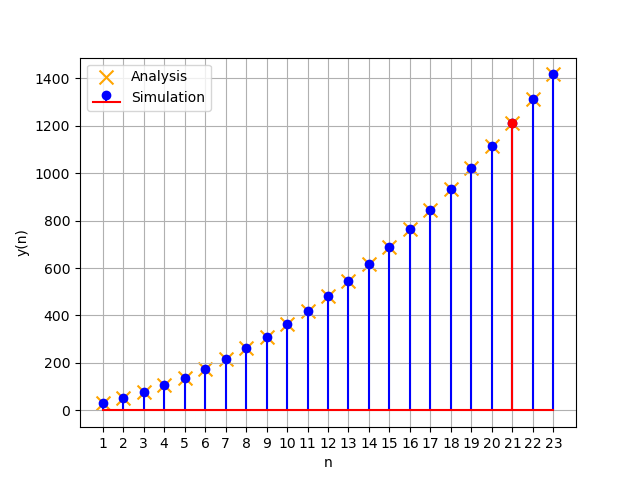
\includegraphics[scale=0.70]{./figs/fig1.png}
    \caption{ }
    \label{fig:x(n) & y(n) }
\end{figure}


\end{document}


\item Check whether -150 is a term of the AP: 11,8,5,2,....

 \solution
 \iffalse
\let\negmedspace\undefined
\let\negthickspace\undefined
\documentclass[journal,12pt,onecolumn]{IEEEtran}
\usepackage{cite}
\usepackage{amsmath,amssymb,amsfonts,amsthm}
\usepackage{algorithmic}
\usepackage{graphicx}
\usepackage{textcomp}
\usepackage{xcolor}
\usepackage{txfonts}
\usepackage{listings}
\usepackage{enumitem}
\usepackage{mathtools}
\usepackage{gensymb}
\usepackage{comment}
\usepackage[breaklinks=true]{hyperref}
\usepackage{tkz-euclide} % loads  TikZ and tkz-base
\usepackage{listings}
\usepackage[latin1]{inputenc}                                
\usepackage{color}                                            
\usepackage{array}                                            
\usepackage{longtable}                                       
\usepackage{calc}                                             
\usepackage{multirow}                                         
\usepackage{hhline}                                           
\usepackage{ifthen}                                           
\usepackage{lscape}
\usepackage{caption}


\newtheorem{theorem}{Theorem}[section]
\newtheorem{problem}{Problem}
\newtheorem{proposition}{Proposition}[section]
\newtheorem{lemma}{Lemma}[section]
\newtheorem{corollary}[theorem]{Corollary}
\newtheorem{example}{Example}[section]
\newtheorem{definition}[problem]{Definition}
%\newtheorem{thm}{Theorem}[section] 
%\newtheorem{defn}[thm]{Definition}
%\newtheorem{algorithm}{Algorithm}[section]
%\newtheorem{cor}{Corollary}
\newcommand{\BEQA}{\begin{eqnarray}}
\newcommand{\EEQA}{\end{eqnarray}}
\newcommand{\define}{\stackrel{\triangle}{=}}
\theoremstyle{remark}
\newtheorem{rem}{Remark}
%\bibliographystyle{ieeetr}

\begin{document}

%
\providecommand{\pr}[1]{\ensuremath{\Pr\left(#1\right)}}
\providecommand{\prt}[2]{\ensuremath{p_{#1}^{\left(#2\right)} }}        % own macro for this question
\providecommand{\qfunc}[1]{\ensuremath{Q\left(#1\right)}}
\providecommand{\sbrak}[1]{\ensuremath{{}\left[#1\right]}}
\providecommand{\lsbrak}[1]{\ensuremath{{}\left[#1\right.}}
\providecommand{\rsbrak}[1]{\ensuremath{{}\left.#1\right]}}
\providecommand{\brak}[1]{\ensuremath{\left(#1\right)}}
\providecommand{\lbrak}[1]{\ensuremath{\left(#1\right.}}
\providecommand{\rbrak}[1]{\ensuremath{\left.#1\right)}}
\providecommand{\cbrak}[1]{\ensuremath{\left\{#1\right\}}}
\providecommand{\lcbrak}[1]{\ensuremath{\left\{#1\right.}}
\providecommand{\rcbrak}[1]{\ensuremath{\left.#1\right\}}}
\newcommand{\sgn}{\mathop{\mathrm{sgn}}}
\providecommand{\abs}[1]{\left\vert#1\right\vert}
\providecommand{\res}[1]{\Res\displaylimits_{#1}} 
\providecommand{\norm}[1]{\left\lVert#1\right\rVert}
%\providecommand{\norm}[1]{\lVert#1\rVert}
\providecommand{\mtx}[1]{\mathbf{#1}}
\providecommand{\mean}[1]{E\left[ #1 \right]}
\providecommand{\cond}[2]{#1\middle|#2}
\providecommand{\fourier}{\overset{\mathcal{F}}{ \rightleftharpoons}}
\newenvironment{amatrix}[1]{%
  \left(\begin{array}{@{}*{#1}{c}|c@{}}
}{%
  \end{array}\right)
}
%\providecommand{\hilbert}{\overset{\mathcal{H}}{ \rightleftharpoons}}
%\providecommand{\system}{\overset{\mathcal{H}}{ \longleftrightarrow}}
        %\newcommand{\solution}[2]{\textbf{Solution:}{#1}}
\newcommand{\solution}{\noindent \textbf{Solution: }}
\newcommand{\cosec}{\,\text{cosec}\,}
\providecommand{\dec}[2]{\ensuremath{\overset{#1}{\underset{#2}{\gtrless}}}}
\newcommand{\myvec}[1]{\ensuremath{\begin{pmatrix}#1\end{pmatrix}}}
\newcommand{\mydet}[1]{\ensuremath{\begin{vmatrix}#1\end{vmatrix}}}
\newcommand{\myaugvec}[2]{\ensuremath{\begin{amatrix}{#1}#2\end{amatrix}}}
\providecommand{\rank}{\text{rank}}
\providecommand{\pr}[1]{\ensuremath{\Pr\left(#1\right)}}
\providecommand{\qfunc}[1]{\ensuremath{Q\left(#1\right)}}
        \newcommand*{\permcomb}[4][0mu]{{{}^{#3}\mkern#1#2_{#4}}}
\newcommand*{\perm}[1][-3mu]{\permcomb[#1]{P}}
\newcommand*{\comb}[1][-1mu]{\permcomb[#1]{C}}
\providecommand{\qfunc}[1]{\ensuremath{Q\left(#1\right)}}
\providecommand{\gauss}[2]{\mathcal{N}\ensuremath{\left(#1,#2\right)}}
\providecommand{\diff}[2]{\ensuremath{\frac{d{#1}}{d{#2}}}}
\providecommand{\myceil}[1]{\left \lceil #1 \right \rceil }
\newcommand\figref{Fig.~\ref}
\newcommand\tabref{Table~\ref}
\newcommand{\sinc}{\,\text{sinc}\,}
\newcommand{\rect}{\,\text{rect}\,}
%%
%       %\newcommand{\solution}[2]{\textbf{Solution:}{#1}}
%\newcommand{\solution}{\noindent \textbf{Solution: }}
%\newcommand{\cosec}{\,\text{cosec}\,}
%\numberwithin{equation}{section}
%\numberwithin{equation}{subsection}
%\numberwithin{problem}{section}
%\numberwithin{definition}{section}
%\makeatletter
%\@addtoreset{figure}{problem}
%\makeatother

%\let\StandardTheFigure\thefigure
\let\vec\mathbf

\bibliographystyle{IEEEtran}

\vspace{3cm}
\title{Assignment}
\author{EE23BTECH11001 - Aashna Sahu}
\maketitle
\bigskip

\renewcommand{\thefigure}{\theenumi}
\renewcommand{\thetable}{\theenumi}
%\renewcommand{\theequation}{\theenumi}
Q:Check whether -150 is a term of the AP: 11,8,5,2,....

 \solution
 \fi

\begin{align}
x(n)&=x(0)+nd\\
n&=\frac{x(n)-x(0)}{d}
\end{align}
\begin{align}
x(n)-x(0) &\equiv 0 \pmod{d}
\end{align}
On substitutings values\\
\begin{align}
-161 &\equiv 2 \pmod{-3}
\end{align}
Thus -150 is not a term of the given AP.
\begin{align}
 \boxed{x(n)=(11-3n)\times u(n)}   
\end{align}

\begin{align}
   X(z)&=\frac{11}{1-z^{-1}}-\frac{3z^{-1}}{(1-z^{-1})^2}\quad
    |z|>1
\end{align}

    \begin{table}[h]
    \centering
    
        \begin{tabular}{|c|c|c|}
      \hline
      Variable & Description & Value\\\hline
      $x(0)$ & First term of AP & 11\\\hline
      $d$ & Common difference & -3\\\hline
      $x(n)$ & General term of given AP & None\\\hline
      \end{tabular}

        
    \caption{Input parameters}
    \label{tab:Table1}
\end{table}
\newpage
\begin{figure}[h]
  \centering
  \includegraphics[width=1.2\columnwidth]{figs/Figure_1.png}
  \captionsetup {justification=centering}
  \caption{Representation of x(n)}
  \label{fig:fig1}
\end{figure}
%\end{document}

 

 \item Write the first five terms of the sequence \(a_n = \frac{n(n^2+5)}{4}\).

\solution
\iffalse
\let\negmedspace\undefined
\let\negthickspace\undefined
\documentclass[journal,12pt,onecolumn]{IEEEtran}
\usepackage{cite}
\usepackage{amsmath,amssymb,amsfonts,amsthm}
\usepackage{algorithmic}
\usepackage{graphicx}
\usepackage{textcomp}
\usepackage{xcolor}
\usepackage{txfonts}
\usepackage{listings}
\usepackage{enumitem}
\usepackage{mathtools}
\usepackage{gensymb}

\usepackage{tkz-euclide} % loads  TikZ and tkz-base
\usepackage{listings}



\newtheorem{theorem}{Theorem}[section]
\newtheorem{problem}{Problem}
\newtheorem{proposition}{Proposition}[section]
\newtheorem{lemma}{Lemma}[section]
\newtheorem{corollary}[theorem]{Corollary}
\newtheorem{example}{Example}[section]
\newtheorem{definition}[problem]{Definition}
%\newtheorem{thm}{Theorem}[section] 
%\newtheorem{defn}[thm]{Definition}
%\newtheorem{algorithm}{Algorithm}[section]
%\newtheorem{cor}{Corollary}
\newcommand{\BEQA}{\begin{eqnarray}}
\newcommand{\EEQA}{\end{eqnarray}}
\newcommand{\system}[1]{\stackrel{#1}{\rightarrow}}

\newcommand{\define}{\stackrel{\triangle}{=}}
\theoremstyle{remark}
\newtheorem{rem}{Remark}
%\bibliographystyle{ieeetr}
\begin{document}
%
\providecommand{\pr}[1]{\ensuremath{\Pr\left(#1\right)}}
\providecommand{\prt}[2]{\ensuremath{p_{#1}^{\left(#2\right)} }}        % own macro for this question
\providecommand{\qfunc}[1]{\ensuremath{Q\left(#1\right)}}
\providecommand{\sbrak}[1]{\ensuremath{{}\left[#1\right]}}
\providecommand{\lsbrak}[1]{\ensuremath{{}\left[#1\right.}}
\providecommand{\rsbrak}[1]{\ensuremath{{}\left.#1\right]}}
\providecommand{\brak}[1]{\ensuremath{\left(#1\right)}}
\providecommand{\lbrak}[1]{\ensuremath{\left(#1\right.}}
\providecommand{\rbrak}[1]{\ensuremath{\left.#1\right)}}
\providecommand{\cbrak}[1]{\ensuremath{\left\{#1\right\}}}
\providecommand{\lcbrak}[1]{\ensuremath{\left\{#1\right.}}
\providecommand{\rcbrak}[1]{\ensuremath{\left.#1\right\}}}
\newcommand{\sgn}{\mathop{\mathrm{sgn}}}
\providecommand{\abs}[1]{\left\vert#1\right\vert}
\providecommand{\res}[1]{\Res\displaylimits_{#1}} 
\providecommand{\norm}[1]{\left\lVert#1\right\rVert}
%\providecommand{\norm}[1]{\lVert#1\rVert}
\providecommand{\mtx}[1]{\mathbf{#1}}
\providecommand{\mean}[1]{E\left[ #1 \right]}
\providecommand{\cond}[2]{#1\middle|#2}
\providecommand{\fourier}{\overset{\mathcal{F}}{ \rightleftharpoons}}
\newenvironment{amatrix}[1]{%
  \left(\begin{array}{@{}*{#1}{c}|c@{}}
}{%
  \end{array}\right)
}
%\providecommand{\hilbert}{\overset{\mathcal{H}}{ \rightleftharpoons}}
%\providecommand{\system}{\overset{\mathcal{H}}{ \longleftrightarrow}}
	%\newcommand{\solution}[2]{\textbf{Solution:}{#1}}
\newcommand{\solution}{\noindent \textbf{Solution: }}
\newcommand{\cosec}{\,\text{cosec}\,}
\providecommand{\dec}[2]{\ensuremath{\overset{#1}{\underset{#2}{\gtrless}}}}
\newcommand{\myvec}[1]{\ensuremath{\begin{pmatrix}#1\end{pmatrix}}}
\newcommand{\mydet}[1]{\ensuremath{\begin{vmatrix}#1\end{vmatrix}}}
\newcommand{\myaugvec}[2]{\ensuremath{\begin{amatrix}{#1}#2\end{amatrix}}}
\providecommand{\rank}{\text{rank}}
\providecommand{\pr}[1]{\ensuremath{\Pr\left(#1\right)}}
\providecommand{\qfunc}[1]{\ensuremath{Q\left(#1\right)}}
	\newcommand*{\permcomb}[4][0mu]{{{}^{#3}\mkern#1#2_{#4}}}
\newcommand*{\perm}[1][-3mu]{\permcomb[#1]{P}}
\newcommand*{\comb}[1][-1mu]{\permcomb[#1]{C}}
\providecommand{\qfunc}[1]{\ensuremath{Q\left(#1\right)}}
\providecommand{\gauss}[2]{\mathcal{N}\ensuremath{\left(#1,#2\right)}}
\providecommand{\diff}[2]{\ensuremath{\frac{d{#1}}{d{#2}}}}
\providecommand{\myceil}[1]{\left \lceil #1 \right \rceil }
\newcommand\figref{Fig.~\ref}
\newcommand\tabref{Table~\ref}
\newcommand{\sinc}{\,\text{sinc}\,}
\newcommand{\rect}{\,\text{rect}\,}
%%
%	%\newcommand{\solution}[2]{\textbf{Solution:}{#1}}
%\newcommand{\solution}{\noindent \textbf{Solution: }}
%\newcommand{\cosec}{\,\text{cosec}\,}
%\numberwithin{equation}{section}
%\numberwithin{equation}{subsection}
%\numberwithin{problem}{section}
%\numberwithin{definition}{section}
%\makeatletter
%\@addtoreset{figure}{problem}
%\makeatother

%\let\StandardTheFigure\thefigure
\let\vec\mathbf

\bibliographystyle{IEEEtran}





\bigskip

\renewcommand{\thefigure}{\theenumi}
\renewcommand{\thetable}{\theenumi}
%\renewcommand{\theequation}{\theenumi}


\title{Discrete Assignment}
\author{Karyampudi Meghana Sai\\ EE23BTECH11031}
\maketitle


Write the first five terms of the sequence \(a_n = \frac{n(n^2+5)}{4}\).

\solution
\fi
\begin{align}
 x(n) &= \left(\frac{n^3+3n^2+8n+6}{4}\right) u(n)\label{eq:1}
\end{align}
\begin{align}
 n^k u(n) \system{Z} (-1)^k z^k \frac{d^k}{dz^k}U(z)
\end{align}

\begin{align}
    nu(n) &\system{Z} \frac{z^{-1}}{(1 - z^{-1})^2} \quad \abs{ z} > 1  \label{eq:3} \\
    n^2u(n) &\system{Z} \frac{(z^{-1})(1+z^{-1})}{(1 - z^{-1})^3} \quad \abs{ z} > 1  \label{eq:4} \\
    n^3u(n) &\system{Z} \frac{(z^{-1})(1+4z^{-1}+z^{-2})}{(1 - z^{-1})^4} \quad \abs{ z} > 1  \label{eq:5} 
\end{align}
Referencing the equations from \eqref{eq:3}, \eqref{eq:4}, and \eqref{eq:5}.
\begin{align}
    x(n) &\system{Z} \frac{(z^{-1})(1+4z^{-1}+z^{-2})}{4(1-z^{-1})^4} + \frac{3(z^{-1})(1+z^{-1})}{4(1-z^{-1})^3} + \frac{2z^{-1}}{(1 - z^{-1})^2} + \frac{3}{2(1- z^{-1})} \quad \abs{ z} > 1  \label{eq:6} \\
    x(n) &\system{Z} \frac{3}{2(1-z^{-1})^3} + \frac{3z^{-2}}{2(1-z^{-1})^4}\quad \abs{ z} > 1  \label{eq:} 
\end{align}

\begin{figure}[h]
    \centering
    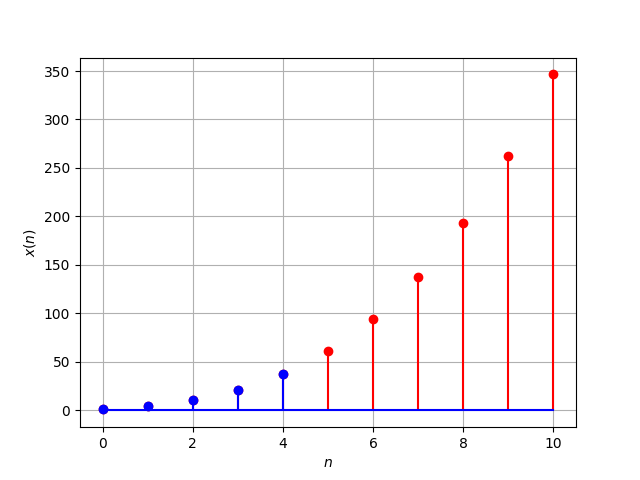
\includegraphics[width=\columnwidth]{ncert-maths/11/9/1/6/figs/plot_from_c.png}
    \caption{Plot of equation\eqref{eq:1}}
    \label{fig:}
\end{figure}
%\end{document}




\item
\begin{enumerate}
\item 30th term of the AP: 10, 7, 4, $\ldots$ is 
\item 11th term of the AP: $-3, -\frac{1}{2}, 2, \ldots$ is
\end{enumerate}
\solution
\iffalse
\let\negmedspace\undefined
\let\negthickspace\undefined
\documentclass[journal,12pt,twocolumn]{IEEEtran}
\usepackage{cite}
\usepackage{amsmath,amssymb,amsfonts,amsthm}
\usepackage{algorithmic}
\usepackage{graphicx}
\usepackage{textcomp}
\usepackage{xcolor}
\usepackage{txfonts}
\usepackage{listings}
\usepackage{enumitem}
\usepackage{mathtools}
\usepackage{gensymb}
\usepackage{comment}
\usepackage[breaklinks=true]{hyperref}
\usepackage{tkz-euclide}
\usepackage{listings}
\usepackage{gvv}
\def\inputGnumericTable{}
\usepackage[latin1]{inputenc}
\usepackage{color}
\usepackage{array}
\usepackage{longtable}
\usepackage{calc}
\usepackage{multirow}
\usepackage{hhline}
\usepackage{ifthen}
\usepackage{lscape}

\newtheorem{theorem}{Theorem}[section]
\newtheorem{problem}{Problem}
\newtheorem{proposition}{Proposition}[section]
\newtheorem{lemma}{Lemma}[section]
\newtheorem{corollary}[theorem]{Corollary}
\newtheorem{example}{Example}[section]
\newtheorem{definition}[problem]{Definition}
\newcommand{\BEQA}{\begin{eqnarray}}
\newcommand{\EEQA}{\end{eqnarray}}
\newcommand{\define}{\stackrel{\triangle}{=}}
\theoremstyle{remark}
\newtheorem{rem}{Remark}
\begin{document}

\bibliographystyle{IEEEtran}
\vspace{3cm}

\title{NCERT Discrete - 10.5.2.2}
\author{EE23BTECH11058 - Sindam Ananya$^{*}$% <-this % stops a space
}
\maketitle
\newpage
\bigskip

\renewcommand{\thefigure}{\theenumi}
\renewcommand{\thetable}{\theenumi}

\vspace{3cm}
\textbf{Question 10.5.2.2:} 
\begin{enumerate}
\item 30th term of the AP: 10, 7, 4, $\ldots$ is 
\item 11th term of the AP: $-3, -\frac{1}{2}, 2, \ldots$ is
\end{enumerate}
\solution
\fi
\begin{table}[h!]
    \centering
    \begin{tabular}{ | c | c | c | }
        \hline
        \textbf{Parameter}  & \textbf{value} & \textbf{Description} \\
        \hline
        \multirow{2}{*}{\begin{tabular}[c]{@{}c@{}}$x_i(0)$\\  \end{tabular}} & 10 & \multirow{2}{*}{\begin{tabular}[c]{@{}c@{}}First \\ term\end{tabular}} \\
        \cline{2-2}
        & -3 &  \\
        \hline
        \multirow{2}{*}{\begin{tabular}[c]{@{}c@{}}$d_i$ \\ \end{tabular}} & -3 & \multirow{2}{*}{\begin{tabular}[c]{@{}c@{}}Common \\ difference\end{tabular}} \\
        \cline{2-2}
          & $\frac{5}{2}$ &  \\
        \hline
        $x_1(29)$ &  ? & 30th term \\
        \hline
        $x_2(10)$ & ? & 11th term \\
        \hline
    \end{tabular}

    \caption{Input Parameters}
    \label{tab:table1}
    \end{table}
\begin{equation}
    x_i(n) = \sbrak{x_i(0) + nd_i} u(n)
    \label{eq:eq1}
\end{equation}
\begin{enumerate}
\item From \eqref{eq:eq1} \tabref{tab:table1} :
\begin{align}
x_1(n) &= \sbrak{10 -3n}u(n)\\
x_1(29) &= -77\\
X_1(z) &= \frac{10 - 13z^{-1}}{(1-z^{-1})^2} \quad \abs{z} > 1
\end{align}
\item From \eqref{eq:eq1} and \tabref{tab:table1} :
\begin{align}
x_2(n) &= \sbrak{-3 + \frac{5}{2}n}u(n)\\
x_2(10) &= 22\\
X_2(z) &= \frac{5.5z^{-1}-3}{(1-z^{-1})^2} \quad \abs{z}> 1
\end{align}
\end{enumerate}
\begin{figure}[h!]
    \centering
    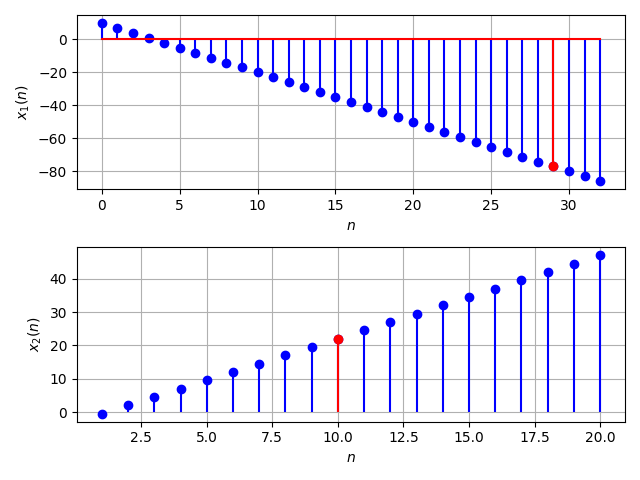
\includegraphics[width=\columnwidth]{ncert-maths/10/5/2/2/figs/plot.png}
    \caption{stem plots of $x_1(n)$ and $x_2(n)$}
    \label{fig:1}
\end{figure}
%\end{document}



\item Write the first five terms of the sequence whose nth term is $\frac{2n-3}{6}$ and obtain the Z transform of the series
\solution
\let\negmedspace\undefined
\let\negthickspace\undefined
\documentclass[journal,12pt,twocolumn]{IEEEtran}
\usepackage{cite}
\usepackage{amsmath,amssymb,amsfonts,amsthm}
\usepackage{algorithmic}
\usepackage{graphicx}
\usepackage{textcomp}
\usepackage{xcolor}
\usepackage{txfonts}
\usepackage{listings}
\usepackage{enumitem}
\usepackage{mathtools}
\usepackage{gensymb}
\usepackage{comment}
\usepackage[breaklinks=true]{hyperref}
\usepackage{tkz-euclide} 
\usepackage{listings}
\usepackage{gvv}                                        
\def\inputGnumericTable{}                                 
\usepackage[latin1]{inputenc}                                
\usepackage{color}                                            
\usepackage{array}                                            
\usepackage{longtable}                                       
\usepackage{calc}                                             
\usepackage{multirow}                                         
\usepackage{hhline}                                           
\usepackage{ifthen}                                           
\usepackage{lscape}

\newtheorem{theorem}{Theorem}[section]
\newtheorem{problem}{Problem}
\newtheorem{proposition}{Proposition}[section]
\newtheorem{lemma}{Lemma}[section]
\newtheorem{corollary}[theorem]{Corollary}
\newtheorem{example}{Example}[section]
\newtheorem{definition}[problem]{Definition}
\newcommand{\BEQA}{\begin{eqnarray}}
\newcommand{\EEQA}{\end{eqnarray}}
\newcommand{\define}{\stackrel{\triangle}{=}}
\theoremstyle{remark}
\newtheorem{rem}{Remark}

\begin{document}
\bibliographystyle{IEEEtran}

\vspace{3cm}

\title{}
\author{EE23BTECH11047 - Deepakreddy P
}
\maketitle
\newpage
\bigskip

\section*{Exercise 9.1}

\noindent \textbf{4} \quad Write the first five terms of the sequence whose nth term is $\frac{2n-3}{6}$ and obtain the Z transform of the series\\
\solution
\begin{align}
x \brak{n} &= \frac{2n-1}{6} \brak{u\brak{n}}
\label{x(n)}
\end{align}

\begin{figure}[h]
   \centering
   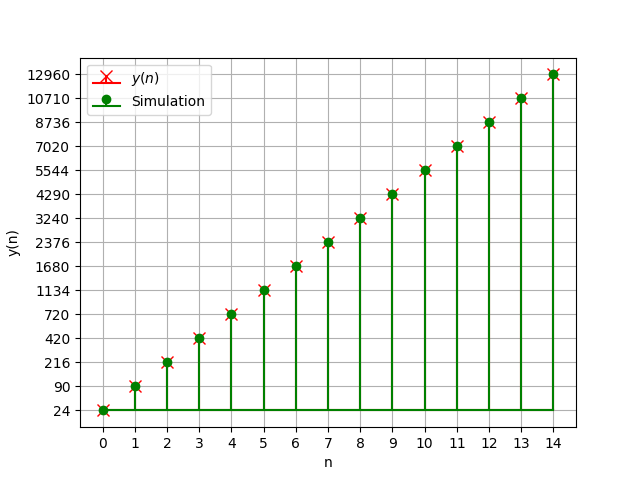
\includegraphics[width=1\columnwidth]{figs/plot.png}
   \caption{Plot of x(n) vs n}
   \label{fig: 9.1.4.1}
\end{figure}

\begin{align}
X(z) &= {\frac{3z^{-1}-1}{6(1-z^{-1})^{2}}\quad|z|>1}
\end{align}


\end{document}


 \item For what values of x, the numbers $-\frac{2}{7}\,,x,-\frac{7}{2}\,$ are in G.P ?

\solution
\iffalse
\let\negmedspace\undefined
\let\negthickspace\undefined
\documentclass[journal,12pt,twocolumn]{IEEEtran}
\usepackage{cite}
\usepackage{amsmath,amssymb,amsfonts,amsthm}
\usepackage{algorithmic}
\usepackage{graphicx}
\usepackage{textcomp}
\usepackage[justification=centering]{caption}
\usepackage{xcolor}
\usepackage{txfonts}
\usepackage{listings}
\usepackage{enumitem}
\usepackage{mathtools}
\usepackage{gensymb}
\usepackage{comment}
\usepackage[breaklinks=true]{hyperref}
\usepackage{tkz-euclide} 
\usepackage{listings}
\usepackage{gvv}                                        
\def\inputGnumericTable{}                                 
\usepackage[latin1]{inputenc}                                
\usepackage{color}                                            
\usepackage{array}                                            
\usepackage{longtable}                                       
\usepackage{calc}                                             
\usepackage{multirow}                                         
\usepackage{hhline}                                           
\usepackage{ifthen}                                           
\usepackage{lscape}

\newtheorem{theorem}{Theorem}[section]
\newtheorem{problem}{Problem}
\newtheorem{proposition}{Proposition}[section]
\newtheorem{lemma}{Lemma}[section]
\newtheorem{corollary}[theorem]{Corollary}
\newtheorem{example}{Example}[section]
\newtheorem{definition}[problem]{Definition}
\newcommand{\BEQA}{\begin{eqnarray}}
\newcommand{\EEQA}{\end{eqnarray}}
\newcommand{\define}{\stackrel{\triangle}{=}}
\theoremstyle{remark}
\newtheorem{rem}{Remark}
\begin{document}

\bibliographystyle{IEEEtran}
\vspace{3cm}

\title{11.9.3.6}
\author{EE23BTECH11022 - G DILIP REDDY}
\maketitle
\newpage

\bigskip

\renewcommand{\thefigure}{\theenumi}
\renewcommand{\thetable}{\theenumi}
\textbf{Question}:\\
For what values of x, the numbers $-\frac{2}{7}\,,x,-\frac{7}{2}\,$ are in G.P ?
\\\\
\textbf{Solution: }\\
\fi
\begin{table}[h]
    \centering
    \renewcommand\thetable{1}
    \begin{tabular}[12.1pt]{ |c| c| c|}
    \hline
    \textbf{Variable} & \textbf{Description} &\textbf{Value}\\ 
    \hline
    $x(0)$ & First term of the GP &$-\brak{\frac{2}{7}}$ \\
    \hline 
    $x(1)$ & Second term of the GP &$x$ \\
    \hline 
    $x(2)$ & Third term of the GP &$-\brak{\frac{7}{2}}$ \\
    \hline 
    $r$ & Common ratio of the GP & \\
    \hline
    $x(n)$ & General term & $x(0)\,r^n\,u(n)$\\
    \hline    
\end{tabular}

    \caption{Variables Used}
    \label{tab:table_11.9.3.6}
\end{table}
Let $r$ be the common ratio\\
From \tabref{tab:table_11.9.3.6}:
\begin{align}
\implies \frac{x}{\brak{-\frac{2}{7}\,}}\,&= \frac{\brak{-\frac{7}{2}\,}}{x}\,=r \\
x^2&=\brak{-\frac{2}{7}\,}\cdot\brak{-\frac{7}{2}\,}\\
x&=\pm 1\\
\implies r&=\pm \frac{7}{2}\,\\\notag
\end{align}
The signal corresponding to this is 
\begin{align}
x(n)=\brak{-\frac{2}{7}}\brak{\pm \frac{7}{2}}^n\,u(n)
\end{align}
Applying z-Transform :
\begin{align}
\implies X_1(z)&=\brak{\frac{1}{7}}\brak{\frac{4}{7z^{-1}+2}\,}
\quad \abs{z}>\frac{7}{2}\\
\implies X_2(z)&=\brak{\frac{1}{7}}\brak{\frac{4}{7z^{-1}-2}\,}
\quad \abs{z}>\frac{7}{2}
\end{align}
\begin{figure}[h]
    \renewcommand\thefigure{1}
    \centering
    \captionsetup{justification=centering}
    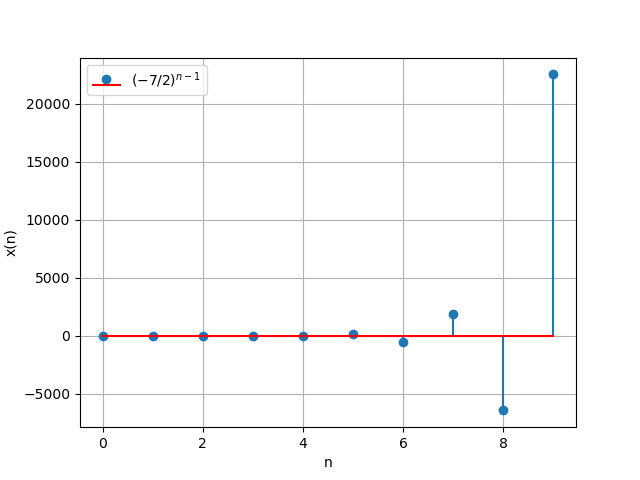
\includegraphics[width=1.1\linewidth]{ncert-maths/11/9/3/6/figs/graph1.png}
    \caption{Stem Plot of $x_1$(n)}
    \label{stemplot1}
\end{figure}
\begin{figure}[h]
    \renewcommand\thefigure{2}
    \centering
    \captionsetup{justification=centering}
    \includegraphics[width=1.1\linewidth]{ncert-maths/11/9/3/6/figs/graph2.png}
    \caption{Stem Plot of $x_2(n)$}
    \label{stemplot2}
\end{figure}
%\end{document}



\item Find the $20^{th}$ and $n^{th}$ terms of the G.P $\frac{5}{2}$, $\frac{5}{4}$, $\frac{5}{8}$,.....

\solution
 \iffalse
\let\negmedspace\undefined
\let\negthickspace\undefined
\documentclass[journal,12pt,twocolumn]{IEEEtran}
\usepackage{cite}
\usepackage{amsmath,amssymb,amsfonts,amsthm}
\usepackage{algorithmic}
\usepackage{graphicx}
\usepackage{textcomp}
\usepackage{xcolor}
\usepackage{txfonts}
\usepackage{listings}
\usepackage{enumitem}
\usepackage{mathtools}
\usepackage{gensymb}
\usepackage{comment}
\usepackage[breaklinks=true]{hyperref}
\usepackage{tkz-euclide} 
\usepackage{listings}
\usepackage{gvv}                                        
\def\inputGnumericTable{}                                 
\usepackage[latin1]{inputenc}                                
\usepackage{color}                                            
\usepackage{array}                                            
\usepackage{longtable}                                       
\usepackage{calc}                                             
\usepackage{multirow}                                         
\usepackage{hhline}                                           
\usepackage{ifthen}                                           
\usepackage{lscape}
\usepackage{caption}
\newtheorem{theorem}{Theorem}[section]
\newtheorem{problem}{Problem}
\newtheorem{proposition}{Proposition}[section]
\newtheorem{lemma}{Lemma}[section]
\newtheorem{corollary}[theorem]{Corollary}
\newtheorem{example}{Example}[section]
\newtheorem{definition}[problem]{Definition}
\newcommand{\BEQA}{\begin{eqnarray}}
\newcommand{\EEQA}{\end{eqnarray}}
\newcommand{\define}{\stackrel{\triangle}{=}}
\theoremstyle{remark}
\newtheorem{rem}{Remark}
\begin{document}
\parindent 0px
\bibliographystyle{IEEEtran}
\vspace{3cm}

\title{NCERT 11.9.3 1Q}
\author{EE23BTECH11013 - Avyaaz$^{*}$% <-this % stops a space
}
\maketitle
\newpage
\bigskip

\renewcommand{\thefigure}{\arabic{figure}}
\renewcommand{\thetable}{\arabic{table}}
\large\textbf{\textsl{Question:}}
Find the $20^{th}$ and $n^{th}$ terms of the G.P $\frac{5}{2}$, $\frac{5}{4}$, $\frac{5}{8}$,.....

\solution
\fi
 \begin{table}[htbp]
     \centering
     \setlength{\extrarowheight}{8pt}
    \begin{table}[ht]
    \centering
    \begin{tabular}{|c|c|c|}
        \hline
        Parameter & Value & Description \\
        \hline
        $x(0)$ & 5 & First term of AP \\
        $d$ & 1.75 & Common difference of AP \\
        $x(n)$ & 20.75 & $n^{th}$ term of AP \\
        \hline
    \end{tabular}
    \vspace{2mm}
    \caption{Parameter List}
    \label{tab:simple.10.5.2.20}
\end{table}

     \caption{Parameters}
     \label{tab:table1}
 \end{table} 

% \begin{align}
%    x(n) = \dfrac{5}{2}\left(\dfrac{1}{2}\right)^n 
% \end{align}

% \begin{align}
% 	x \brak{n} & \system{Z} X \brak{z} \\
%    % x(n) &=\dfrac{5}{2}\left(\dfrac{1}{2}\right)^n u(n) \\
%     \therefore X(z) &= \sum_{n=-\infty}^{\infty}x(n)z^{-n}\label{eq:z-transform}  
% \end{align}
% Here, 
%          $    u(n) = \begin{cases}
%                 0 &\text{for } n < 0 \\
%                 1 & \text{for } n \geq 0
%             \end{cases}$       
 
%  \vspace{1cm}
From \tabref{tab:table1}:
\(Z\)-Transform of \(x(n)\):
\begin{align}
% \implies X(z) &= \sum_{n=-\infty}^{\infty}\left(\dfrac{5}{2}\left(\dfrac{1}{2}\right)^n u(n)\right) z^{-n} \\
 % \implies X(z) &= \dfrac{5}{2}\sum_{n=0}^{\infty}\left(\dfrac{z
 % ^{-1}}{2}\right)^n \\
\implies X(z) &=\dfrac{5}{2}\left(\dfrac{1}{1-\frac{z^{-1}}{2}}\right) ;\cbrak{z\in\mathbb{C} : |z|>\dfrac{1}{2}}
\end{align}

\begin{figure}[ht]
    \centering
    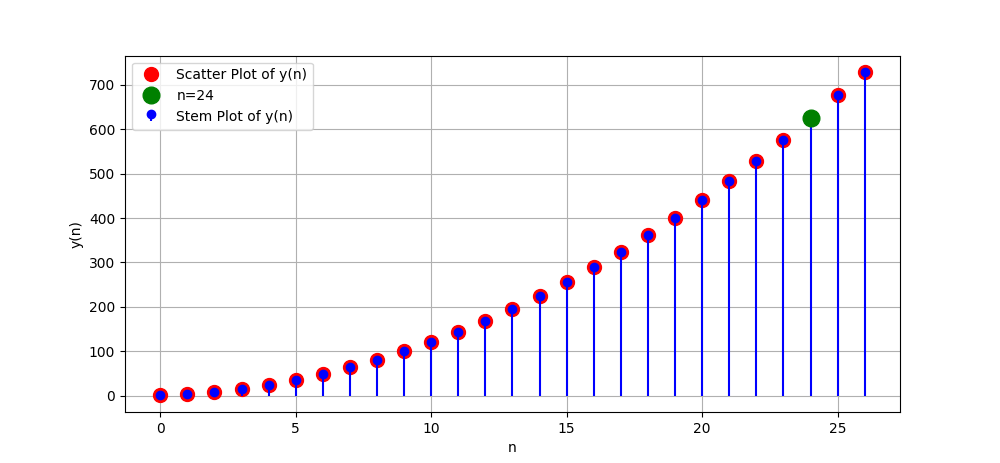
\includegraphics[width = \columnwidth]{figs/stem_plot.png}
    \caption{}
    \label{fig:graph1}
\end{figure} 

\bibliographystyle{IEEEtran}
%\end{document}



\item 
Which term of the following sequences:\\
(a) 2,$2\sqrt{2}$,4\dots is 128
\quad(b) $\sqrt{3}$,3,$3\sqrt{3}$\dots is 729\\
(c) $\frac{1}{3}$,$\frac{1}{9}$,$\frac{1}{27}$\dots is $\frac{1}{19683}$ \\
\solution
\iffalse
\let\negmedspace\undefined
\let\negthickspace\undefined
\documentclass[journal,12pt,twocolumn]{IEEEtran}
\usepackage{cite}
\usepackage{amsmath,amssymb,amsfonts,amsthm}
\usepackage{algorithmic}
\usepackage{graphicx}
\usepackage{textcomp}
\usepackage{xcolor}
\usepackage{txfonts}
\usepackage{listings}
\usepackage{enumitem}
\usepackage{mathtools}
\usepackage{gensymb}
\usepackage{comment}
\usepackage[breaklinks=true]{hyperref}
\usepackage{tkz-euclide} 
\usepackage{listings}
\usepackage{gvv}                                        
\def\inputGnumericTable{}                                 
\usepackage[latin1]{inputenc}                                
\usepackage{color}                                            
\usepackage{array}                                            
\usepackage{longtable}                                       
\usepackage{calc}                                             
\usepackage{multirow}                                         
\usepackage{hhline}                                           
\usepackage{ifthen}                                           
\usepackage{lscape}
\usepackage[center]{caption} % center the captions to figure

\newtheorem{theorem}{Theorem}[section]
\newtheorem{problem}{Problem}
\newtheorem{proposition}{Proposition}[section]
\newtheorem{lemma}{Lemma}[section]
\newtheorem{corollary}[theorem]{Corollary}
\newtheorem{example}{Example}[section]
\newtheorem{definition}[problem]{Definition}
\newcommand{\BEQA}{\begin{eqnarray}}
\newcommand{\EEQA}{\end{eqnarray}}
\newcommand{\define}{\stackrel{\triangle}{=}}
\theoremstyle{remark}
\newtheorem{rem}{Remark}
\begin{document}

\newcolumntype{M}[1]{>{\centering\arraybackslash}m{#1}}
\newcolumntype{N}{@{}m{0pt}@{}}

\bibliographystyle{IEEEtran}
\vspace{3cm}

\title{NCERT 11.9.3 5Q} 
\author{ee23btech11223 - Soham Prabhakar More% <-this % stops a space
}
\maketitle
\newpage
\bigskip

\renewcommand{\thefigure}{\theenumi}
\renewcommand{\thetable}{\theenumi}

\bibliographystyle{IEEEtran}

\textbf{Question:}\\
Which term of the following sequences:\\
(a) 2,$2\sqrt{2}$,4\dots is 128
\quad(b) $\sqrt{3}$,3,$3\sqrt{3}$\dots is 729\\
(c) $\frac{1}{3}$,$\frac{1}{9}$,$\frac{1}{27}$\dots is $\frac{1}{19683}$
\fi 
For a general GP series and $k > 0$,
\begin{align}
    x\brak{k} &= x\brak{0}r^k \\
    \therefore k &= \log_r{\frac{x\brak{k}}{x\brak{0}}} \label{eq:gsoln}
\end{align}
And the Z-transform $X\brak{z}$:
\begin{align}
    X\brak{z} &= \frac{x\brak{0}}{1 - rz^{-1}} \quad {\abs{z} > \abs{r}} \label{eq:zresult}
\end{align}

\begin{enumerate}[label=(\alph*)]
\item By \tabref{Table:1}, \eqref{eq:gsoln} and \tabref{Table:1}: % prob:a
\begin{align}
    x_1\brak{n} &= x_1\brak{0} r_1^nu\brak{n} \\
    k_1 &= \log_{r_1}{\frac{128}{x_1\brak{0}}} \\
    \therefore k_1 &= 12 \\
	X_1\brak{z} &= \frac{2}{1 - \sqrt{2}z^{-1}} \quad \abs{z} > \sqrt{2}
\end{align}

\begin{figure}[h!]
    \renewcommand\thefigure{1}
    \centering
    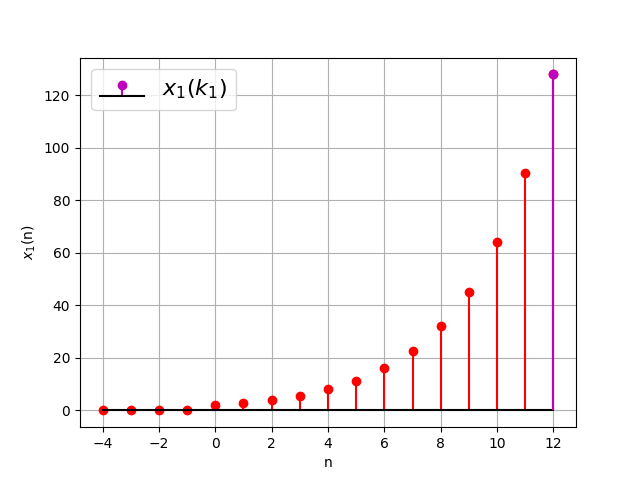
\includegraphics[width=\columnwidth]{ncert-maths/11/9/3/5/figs/a.png}
    \caption[short]{Plot of $x_1$\brak{n} vs n. See \tabref{Table:1}}
    \label{fig:img1}
\end{figure}



\item By \eqref{eq:gsoln}, \eqref{eq:zresult} and \tabref{Table:1}: % prob:b
\begin{align}
    x_2\brak{n} &= x_2\brak{0} r_2^nu\brak{n} \\
    k_2 &= \log_{r_2}{\frac{729}{x_2\brak{0}}} \\
    \therefore k_2 &= 11 \\
    X_2\brak{z} &= \frac{\sqrt{3}}{1 - \sqrt{3}z^{-1}} \quad \abs{z} > \sqrt{3} 
\end{align}

\begin{figure}[h!]
    \renewcommand\thefigure{2}
    \centering
    \includegraphics[width=\columnwidth]{ncert-maths/11/9/3/5/figs/b.png}
    \caption[short]{Plot of $x_2$\brak{n} vs n. See \tabref{Table:1}}
    \label{fig:img2}
\end{figure}

\item By \eqref{eq:gsoln}, \eqref{eq:zresult} and \tabref{Table:1}: % prob:c
\begin{align}
    x_3\brak{n} &= x_3\brak{0} r_3^nu\brak{n} \\
    k_3 &= \log_{r_3}{\frac{1}{19683 x_3\brak{0}}} \\
    \therefore k_3 &= 8 \\
    X_3\brak{z} &= \frac{1}{3 - z^{-1}} \quad \abs{z} > \frac{1}{3}
\end{align}

\begin{figure}[h!]
    \renewcommand\thefigure{3}
    \centering
    \includegraphics[width=\columnwidth]{ncert-maths/11/9/3/5/figs/c.png}
    \caption[short]{Plot of $x_3$\brak{n} vs n. See \tabref{Table:1}}
    \label{fig:img3}
\end{figure}

\begin{table}[ht]
\begin{tabular}{|c|c|c|}
    \hline 
    \textbf{Parameter}&\textbf{Description} &\textbf{Value}\\
    \hline 
    $r_i$ & Common ratio of G.P (a),(b),(c) & $\sqrt{2}, \sqrt{3}, \frac{1}{3}$ \\
    \hline
    $x_i(0)$ & Initial Values & $2, \sqrt{3}, \frac{1}{3}$ \\
    \hline
    $x_i(k_i)$ & Given Values & $128, 729, \frac{1}{19683}$ \\
    \hline 
    $k_i$ & Desired index & $12, 11, 8$ \\
    \hline 
    $x_i\brak{n}$ & Series & $x_i\brak{0}r_i^nu\brak{n}$ \\
    \hline
	$X_i\brak{z}$ & Z-Transform of $x_i\brak{n}$ & $\frac{x\brak{0}}{1-rz^{-1}}$ \\
    \hline
\end{tabular}

\caption{Table of parameters}
\label{Table:1}


\end{table}

\end{enumerate}

Find the $20^{th}$ and $n^{th}$ terms of the G.P $\frac{5}{2}$, $\frac{5}{4}$, $\frac{5}{8}$,.....

% \item 
% Which term of the following sequences:\\
% (a) 2,$2\sqrt{2}$,4\dots is 128
% \quad(b) $\sqrt{3}$,3,$3\sqrt{3}$\dots is 729\\
% (c) $\frac{1}{3}$,$\frac{1}{9}$,$\frac{1}{27}$\dots is $\frac{1}{19683}$
% \solution
% \iffalse
\let\negmedspace\undefined
\let\negthickspace\undefined
\documentclass[journal,12pt,twocolumn]{IEEEtran}
\usepackage{cite}
\usepackage{amsmath,amssymb,amsfonts,amsthm}
\usepackage{algorithmic}
\usepackage{graphicx}
\usepackage{textcomp}
\usepackage{xcolor}
\usepackage{txfonts}
\usepackage{listings}
\usepackage{enumitem}
\usepackage{mathtools}
\usepackage{gensymb}
\usepackage{comment}
\usepackage[breaklinks=true]{hyperref}
\usepackage{tkz-euclide} 
\usepackage{listings}
\usepackage{gvv}                                        
\def\inputGnumericTable{}                                 
\usepackage[latin1]{inputenc}                                
\usepackage{color}                                            
\usepackage{array}                                            
\usepackage{longtable}                                       
\usepackage{calc}                                             
\usepackage{multirow}                                         
\usepackage{hhline}                                           
\usepackage{ifthen}                                           
\usepackage{lscape}
\usepackage[center]{caption} % center the captions to figure

\newtheorem{theorem}{Theorem}[section]
\newtheorem{problem}{Problem}
\newtheorem{proposition}{Proposition}[section]
\newtheorem{lemma}{Lemma}[section]
\newtheorem{corollary}[theorem]{Corollary}
\newtheorem{example}{Example}[section]
\newtheorem{definition}[problem]{Definition}
\newcommand{\BEQA}{\begin{eqnarray}}
\newcommand{\EEQA}{\end{eqnarray}}
\newcommand{\define}{\stackrel{\triangle}{=}}
\theoremstyle{remark}
\newtheorem{rem}{Remark}
\begin{document}

\newcolumntype{M}[1]{>{\centering\arraybackslash}m{#1}}
\newcolumntype{N}{@{}m{0pt}@{}}

\bibliographystyle{IEEEtran}
\vspace{3cm}

\title{NCERT 11.9.3 5Q} 
\author{ee23btech11223 - Soham Prabhakar More% <-this % stops a space
}
\maketitle
\newpage
\bigskip

\renewcommand{\thefigure}{\theenumi}
\renewcommand{\thetable}{\theenumi}

\bibliographystyle{IEEEtran}

\textbf{Question:}\\
Which term of the following sequences:\\
(a) 2,$2\sqrt{2}$,4\dots is 128
\quad(b) $\sqrt{3}$,3,$3\sqrt{3}$\dots is 729\\
(c) $\frac{1}{3}$,$\frac{1}{9}$,$\frac{1}{27}$\dots is $\frac{1}{19683}$
\fi 
For a general GP series and $k > 0$,
\begin{align}
    x\brak{k} &= x\brak{0}r^k \\
    \therefore k &= \log_r{\frac{x\brak{k}}{x\brak{0}}} \label{eq:gsoln}
\end{align}
And the Z-transform $X\brak{z}$:
\begin{align}
    X\brak{z} &= \frac{x\brak{0}}{1 - rz^{-1}} \quad {\abs{z} > \abs{r}} \label{eq:zresult}
\end{align}

\begin{enumerate}[label=(\alph*)]
\item By \tabref{Table:1}, \eqref{eq:gsoln} and \tabref{Table:1}: % prob:a
\begin{align}
    x_1\brak{n} &= x_1\brak{0} r_1^nu\brak{n} \\
    k_1 &= \log_{r_1}{\frac{128}{x_1\brak{0}}} \\
    \therefore k_1 &= 12 \\
	X_1\brak{z} &= \frac{2}{1 - \sqrt{2}z^{-1}} \quad \abs{z} > \sqrt{2}
\end{align}

\begin{figure}[h!]
    \renewcommand\thefigure{1}
    \centering
    \includegraphics[width=\columnwidth]{ncert-maths/11/9/3/5/figs/a.png}
    \caption[short]{Plot of $x_1$\brak{n} vs n. See \tabref{Table:1}}
    \label{fig:img1}
\end{figure}



\item By \eqref{eq:gsoln}, \eqref{eq:zresult} and \tabref{Table:1}: % prob:b
\begin{align}
    x_2\brak{n} &= x_2\brak{0} r_2^nu\brak{n} \\
    k_2 &= \log_{r_2}{\frac{729}{x_2\brak{0}}} \\
    \therefore k_2 &= 11 \\
    X_2\brak{z} &= \frac{\sqrt{3}}{1 - \sqrt{3}z^{-1}} \quad \abs{z} > \sqrt{3} 
\end{align}

\begin{figure}[h!]
    \renewcommand\thefigure{2}
    \centering
    \includegraphics[width=\columnwidth]{ncert-maths/11/9/3/5/figs/b.png}
    \caption[short]{Plot of $x_2$\brak{n} vs n. See \tabref{Table:1}}
    \label{fig:img2}
\end{figure}

\item By \eqref{eq:gsoln}, \eqref{eq:zresult} and \tabref{Table:1}: % prob:c
\begin{align}
    x_3\brak{n} &= x_3\brak{0} r_3^nu\brak{n} \\
    k_3 &= \log_{r_3}{\frac{1}{19683 x_3\brak{0}}} \\
    \therefore k_3 &= 8 \\
    X_3\brak{z} &= \frac{1}{3 - z^{-1}} \quad \abs{z} > \frac{1}{3}
\end{align}

\begin{figure}[h!]
    \renewcommand\thefigure{3}
    \centering
    \includegraphics[width=\columnwidth]{ncert-maths/11/9/3/5/figs/c.png}
    \caption[short]{Plot of $x_3$\brak{n} vs n. See \tabref{Table:1}}
    \label{fig:img3}
\end{figure}

\begin{table}[ht]
\input{ncert-maths/11/9/3/5/tables/table.tex}
\end{table}

\end{enumerate}

Find the $20^{th}$ and $n^{th}$ terms of the G.P $\frac{5}{2}$, $\frac{5}{4}$, $\frac{5}{8}$,.....

% \item 
% Which term of the following sequences:\\
% (a) 2,$2\sqrt{2}$,4\dots is 128
% \quad(b) $\sqrt{3}$,3,$3\sqrt{3}$\dots is 729\\
% (c) $\frac{1}{3}$,$\frac{1}{9}$,$\frac{1}{27}$\dots is $\frac{1}{19683}$
% \solution
% \input{ncert-maths/11/9/3/5/main.tex}
% \pagebreak

%\end{document}


% \pagebreak

%\end{document}


\clearpage

\item The number of bacteria in a certain culture doubles every hour. If there were 30 bacteria present in the culture originally, how many bacteria will be present at the end of $2^{nd}$ hour, $4^{th}$ hour and $n^{th}$ hour?

\solution
\iffalse
\let\negmedspace\undefined
\let\negthickspace\undefined
\documentclass[journal,12pt,twocolumn]{IEEEtran}
\usepackage{cite}
\usepackage{amsmath,amssymb,amsfonts,amsthm}
\usepackage{algorithmic}
\usepackage{graphicx}
\usepackage{textcomp}
\usepackage{xcolor}
\usepackage{txfonts}
\usepackage{listings}
\usepackage{enumitem}
\usepackage{mathtools}
\usepackage{gensymb}
\usepackage{comment}
\usepackage[breaklinks=true]{hyperref}
\usepackage{tkz-euclide}
\usepackage{listings}
\usepackage{gvv}
\def\inputGnumericTable{}
\usepackage[latin1]{inputenc}
\usepackage{color}
\usepackage{array}
\usepackage{longtable}
\usepackage{calc}
\usepackage{multirow}
\usepackage{hhline}
\usepackage{ifthen}
\usepackage{lscape}

\newtheorem{theorem}{Theorem}[section]
\newtheorem{problem}{Problem}
\newtheorem{proposition}{Proposition}[section]
\newtheorem{lemma}{Lemma}[section]
\newtheorem{corollary}[theorem]{Corollary}
\newtheorem{example}{Example}[section]
\newtheorem{definition}[problem]{Definition}
\newcommand{\BEQA}{\begin{eqnarray}}
\newcommand{\EEQA}{\end{eqnarray}}
\newcommand{\define}{\stackrel{\triangle}{=}}
\theoremstyle{remark}
\newtheorem{rem}{Remark}
\begin{document}

\bibliographystyle{IEEEtran}
\vspace{3cm}

\title{NCERT Discrete - 11.9.3.30}
\author{EE23BTECH11007 - Aneesh Kadiyala$^{*}$% <-this % stops a space
}
\maketitle
\newpage
\bigskip

\renewcommand{\thefigure}{\theenumi}
\renewcommand{\thetable}{\theenumi}

\vspace{3cm}
\textbf{Question 11.9.3.30:} The number of bacteria in a certain culture doubles every hour. If there were 30 bacteria present in the culture originally, how many bacteria will be present at the end of $2^{nd}$ hour, $4^{th}$ hour and $n^{th}$ hour?
\\
\solution
\fi
\begin{table}[h!]
    \begin{tabular}{ | c | c | c | }
    \hline
    Parameter & Value & Description \\
    \hline
    $x(0)$ & 30 & Initial no. of bacteria\\
    \hline
    $r$ & 2 & Ratio of no. of bacteria at end of \\
    & & hour to start of hour (Common Ratio) \\
    \hline
    $x(n)$ & $r^nx(0)u(n)$ & $n^{th}$ term of the GP \\
    \hline
\end{tabular}
    \caption{Input Parameters}
    \label{tab:ncert_maths_11_9_3_30}
\end{table}
From \tabref{tab:ncert_maths_11_9_3_30}:
\begin{align}
x(2) &= 120 \\
x(4) &= 480 \\
x(n) &= 30(2^n)u(n)
\end{align}
\begin{figure}[h!]
    \centering
    \includegraphics[width=\columnwidth]{ncert-maths/11/9/3/30/figs/11_9_3_30.png}
    \caption{Plot of $x(n)$ vs $n$. See \tabref{tab:ncert_maths_11_9_3_30} for details.}
    \label{fig:ncert_maths_11_9_3_30}
\end{figure}
\begin{align}
X(z) = \frac{30z^{-1}}{1 - 2z^{-1}} \quad \abs{z} > 2
\end{align}
%\end{document}


\item Ramkali saved Rs 5 in the first week of a year and then increased her weekly savings by Rs 1.75. If in the $n$th week, her weekly savings become Rs 20.75, find $n$.

\solution
\iffalse
\let\negmedspace\undefined
\let\negthickspace\undefined
\documentclass[journal,12pt,twocolumn]{IEEEtran}
\usepackage{cite}
\usepackage{amsmath,amssymb,amsfonts,amsthm}
\usepackage{algorithmic}
\usepackage{graphicx}
\usepackage{textcomp}
\usepackage{xcolor}
\usepackage{txfonts}
\usepackage{listings}
\usepackage{enumitem}
\usepackage{mathtools}
\usepackage{gensymb}
\usepackage[breaklinks=true]{hyperref}
\usepackage{tkz-euclide} % loads  TikZ and tkz-base
\usepackage{listings}
\usepackage{gvv}


\newtheorem{theorem}{Theorem}[section]
\newtheorem{problem}{Problem}
\newtheorem{proposition}{Proposition}[section]
\newtheorem{lemma}{Lemma}[section]
\newtheorem{corollary}[theorem]{Corollary}
\newtheorem{example}{Example}[section]
\newtheorem{definition}[problem]{Definition}

\newcommand{\BEQA}{\begin{eqnarray}}
\newcommand{\EEQA}{\end{eqnarray}}
\newcommand{\define}{\stackrel{\triangle}{=}}
\theoremstyle{remark}
\newtheorem{rem}{Remark}

\graphicspath{./figs/}

%\bibliographystyle{ieeetr}
\begin{document}
%

\bibliographystyle{IEEEtran}


\vspace{3cm}

\title{
	%	\logo{
	Assignment-1 

	\large{EE:1205 Signals and Systems}

	Indian Institute of Technology, Hyderabad
	%	}
}
\author{Kunal Thorawade

EE23BTECH11035
}	

\maketitle


\newpage

%\tableofcontents

\bigskip
 
 \renewcommand{\thefigure}{\theenumi}
 \renewcommand{\thetable}{\theenumi}
 %\renewcommand{\theequation}{\theenumi}

 \section{\Large Question:}  Ramkali saved Rs 5 in the first week of a year and then increased her weekly savings by Rs 1.75. If in the $n$th week, her weekly savings become Rs 20.75, find $n$.

 \section{\Large Solution:} 
 \fi
 \begin{table}[ht]
    \centering
    \begin{tabular}{|c|c|c|}
        \hline
        Parameter & Value & Description \\
        \hline
        $x(0)$ & 5 & First term of AP \\
        $d$ & 1.75 & Common difference of AP \\
        $x(n)$ & 20.75 & $n^{th}$ term of AP \\
        \hline
    \end{tabular}
    \vspace{2mm}
    \caption{Parameter List}
    \label{tab:simple.10.5.2.20}
\end{table}


 \begin{align} 
	 x(n) &= x(0) + (n)(d)
	 \\ 20.75 &= 5 + (n)(1.75)  
	 \\ \implies 15.75 &= (n)(1.75)
	 \\ \implies n &= \frac{15.75}{1.75}
	 \\ \implies n &= 9
	 \\x(n) &= 5u(n) + 1.75nu(n)
 \end{align}
 The Z-transform of a sequence $x(n)$ is given by:
 \begin{align}
	  X(z) &= \frac{5z^{-1}}{1-z^{-1}}+\frac{1.75z^{-1}}{(1-z^{-1})^{2}} ; |z| > 1
 \end{align}

 \begin{figure}
	     \centering
	         \includegraphics[width = 8cm]{ncert-maths/10/5/2/20/figs/fig1.png}
		     \caption{Plot of $x(n) = 5 + 1.75n$}
		         \label{fig:enter-label.10.5.2.20}
 \end{figure}




\item Show that the sum of $\brak {m+n}^{th}$ and $\brak {m-n}^{th}$ terms of an $A.P.,$ is equal to twice the $m^{th}$ terms.    \\
\solution
\iffalse
\let\negmedspace\undefined
\let\negthickspace\undefined
\documentclass[journal,12pt,twocolumn]{IEEEtran}
\usepackage{cite}
\usepackage{amsmath,amssymb,amsfonts,amsthm}
\usepackage{algorithmic}
\usepackage{graphicx}
\usepackage{textcomp}
\usepackage{xcolor}
\usepackage{txfonts}
\usepackage{listings}
\usepackage{enumitem}
\usepackage{mathtools}
\usepackage{gensymb}
\usepackage{comment}
\usepackage[breaklinks=true]{hyperref}
\usepackage{tkz-euclide} 
\usepackage{listings}
\usepackage{gvv}                                        
\def\inputGnumericTable{}                                 
\usepackage[latin1]{inputenc}                                
\usepackage{color}                                            
\usepackage{array}                                            
\usepackage{longtable}                                       
\usepackage{calc}                                             
\usepackage{multirow}                                         
\usepackage{hhline}                                           
\usepackage{ifthen}                                           
\usepackage{lscape}

\newtheorem{theorem}{Theorem}[section]
\newtheorem{problem}{Problem}
\newtheorem{proposition}{Proposition}[section]
\newtheorem{lemma}{Lemma}[section]
\newtheorem{corollary}[theorem]{Corollary}
\newtheorem{example}{Example}[section]
\newtheorem{definition}[problem]{Definition}
\newcommand{\BEQA}{\begin{eqnarray}}
\newcommand{\EEQA}{\end{eqnarray}}
\newcommand{\define}{\stackrel{\triangle}{=}}
\theoremstyle{remark}
\newtheorem{rem}{Remark}
\begin{document}
\parindent 0px
\bibliographystyle{IEEEtran}
\title{Assignment 11.9.5\_1Q}
\author{EE22BTECH11219 - Rada Sai Sujan$^{}$% <-this % stops a space
}
\maketitle
\newpage
\bigskip
\section*{Question}
Show that the sum of $\brak {m+n}^{th}$ and $\brak {m-n}^{th}$ terms of an $A.P.,$ is equal to twice the $m^{th}$ terms.    \\
\solution
\fi

\begin{table}[ht]
    \centering
    \def\arraystretch{1.5}
    \begin{tabular}{|p{2cm}|p{2.5cm}|p{2.3cm}|}
    \hline
    PARAMETER & VALUE & DESCRIPTION  \\ \hline
    $$x\brak0$$ & $$x\brak{0}$$ & First term \\ \hline
    $$d$$ & $$d$$ & common difference \\ \hline
    $$x(n)$$ & $$[x\brak{0}+nd]u\brak n$$ & General term of the series  \\ \hline
  \end{tabular}

    \caption{Parameter Table1}
    \label{tab:10.9.5.1.1}
\end{table}
For an $AP$,
\begin{align}
    x\brak{n}&=[x\brak{0}+nd]u\brak{n}   \\
    \implies x\brak{m+n}+x\brak{m-n}&=[x\brak{0}+\brak{m+n}d]+[x\brak{0}+\brak{m-n}d] \\
    &=2[x\brak{0}+md]   \\
    \therefore x\brak{m+n}+x\brak{m-n}&=2x\brak{m}
\end{align}
\begin{table}[ht]
    \centering
    \def\arraystretch{1.5}
    \begin{tabular}{|p{4.5cm}|p{4.5cm}|}
    \hline
      $$x\brak{0}$$ & $$3$$  \\ \hline
      $$d$$ & $$2$$  \\ \hline
      $$m$$ & $$6$$  \\ \hline
      $$n$$ & $$2$$  \\ \hline
      $$x\brak{m+n}$$ & $$19$$  \\ \hline
      $$x\brak{m-n}$$ & $$11$$  \\ \hline
      $$x\brak{m}$$ & $$15$$  \\ \hline
    \end{tabular}

    \caption{Verified Values}
    \label{tab:10.9.5.1.2}
\end{table}




\item The sum of the first three terms of a G.P is $39/10$ and their product is $1$. Find the common ratio and the terms.\\
\solution
\iffalse
\let\negmedspace\undefined
\let\negthickspace\undefined
\documentclass[journal,12pt,twocolumn]{IEEEtran}
\usepackage{cite}
\usepackage{amsmath,amssymb,amsfonts,amsthm}
\usepackage{algorithmic}
\usepackage{graphicx}
\usepackage{textcomp}
\usepackage{xcolor}
\usepackage{txfonts}
\usepackage{listings}
\usepackage{enumitem}
\usepackage{mathtools}
\usepackage{gensymb}
\usepackage{comment}
\usepackage[breaklinks=true]{hyperref}
\usepackage{tkz-euclide}
\usepackage{listings}
\usepackage{gvv}
\def\inputGnumericTable{}
\usepackage[latin1]{inputenc}
\usepackage{color}
\usepackage{array}
\usepackage{longtable}
\usepackage{calc}
\usepackage{multirow}
\usepackage{hhline}
\usepackage{ifthen}
\usepackage{lscape}

\newtheorem{theorem}{Theorem}[section]
\newtheorem{problem}{Problem}
\newtheorem{proposition}{Proposition}[section]
\newtheorem{lemma}{Lemma}[section]
\newtheorem{corollary}[theorem]{Corollary}
\newtheorem{example}{Example}[section]
\newtheorem{definition}[problem]{Definition}
\newcommand{\BEQA}{\begin{eqnarray}}
\newcommand{\EEQA}{\end{eqnarray}}
\newcommand{\define}{\stackrel{\triangle}{=}}
\theoremstyle{remark}
\newtheorem{rem}{Remark}
\begin{document}

\bibliographystyle{IEEEtran}
\vspace{3cm}

\title{NCERT Discrete - 11.9.3.12}
\author{EE23BTECH11058 - Sindam Ananya$^{*}$% <-this % stops a space
}
\maketitle
\newpage
\bigskip

\renewcommand{\thefigure}{\theenumi}
\renewcommand{\thetable}{\theenumi}

\vspace{3cm}
\textbf{Question : 11.9.3.12} 
The sum of the first three terms of a G.P is $39/10$ and their product is $1$. Find the common ratio and the terms.\\
\solution
\fi
\begin{table}[h!]
    \centering
    \begin{tabular}{|c|c|c|}
        \hline
        \textbf{Parameter} & \textbf{Value} & \textbf{Description} \\
        \hline
        $x(0)$ & & First term \\
        \hline
        $r$ & & Common ratio \\
        \hline
        $x(0)^3r^3$ & 1 & Product of terms \\
        \hline
        $x(0)$ + $x(0)r$ + $x(0)r^2$ & $\frac{39}{10}$ & Sum of terms \\
        \hline
    \end{tabular}

    \caption{Input Parameters}
    \label{tab:11.9.3.12table1}
\end{table}
\begin{equation}
y(n) = x(0)\brak{\frac{r^{n+1}-1}{r-1}}u(n)
\label{eq:11.9.3.12eq1}
\end{equation}
From \tabref{tab:11.9.3.12table1} and \eqref{eq:11.9.3.12eq1} :
\begin{align}
y(2) &= x(0)\brak{\frac{r^3-1}{r-1}}\\
\frac{39}{10} &= x(0)\brak{r^2+r+1}\\
\implies \frac{39r}{10} &= r^2+r+1 \quad \brak{\because x(0)r = 1}\\
\implies (2r-5)(5r-2) &=0\\
\implies r &= \frac{2}{5} \quad or \quad \frac{5}{2}
\end{align}
\begin{enumerate}
      \item If $r = \frac{2}{5}$, then terms are $\frac{5}{2}$, $1$, $\frac{2}{5}$.
      \item If $r = \frac{5}{2}$, then terms are $\frac{2}{5}$, $1$, $\frac{5}{2}$.
\end{enumerate}
\begin{figure}[h!]
    \centering
    \includegraphics[width=\columnwidth]{ncert-maths/11/9/3/12/figs/graph1.png}
    \caption{stem plots of GP if $r=\frac{2}{5}$}
    \label{fig:11.9.3.12_1}
\end{figure}
\begin{figure}[h!]
    \centering
    \includegraphics[width=\columnwidth]{ncert-maths/11/9/3/12/figs/graph2.png}
    \caption{stem plots of GP if $r=\frac{5}{2}$}
    \label{fig:11.9.3.12_2}
\end{figure}
%\end{document}




\item The ratio of the A.M and G.M of two positive numbers $a$ and $b$ is $m:n$. Show that $a:b = \brak{ m + \sqrt{m^2 - n^2}} : \brak{ m - \sqrt{m^2 - n^2}}$.\\
\solution
\let\negmedspace\undefined
\let\negthickspace\undefined
\documentclass[journal,12pt,onecolumn]{IEEEtran}
\usepackage{cite}
\usepackage{amsmath,amssymb,amsfonts,amsthm}
\usepackage{algorithmic}
\usepackage{graphicx}
\usepackage{textcomp}
\usepackage{xcolor}
\usepackage{txfonts}
\usepackage{listings}
\usepackage{enumitem}
\usepackage{mathtools}
\usepackage{gensymb}

\usepackage{tkz-euclide} % loads  TikZ and tkz-base
\usepackage{listings}



\newtheorem{theorem}{Theorem}[section]
\newtheorem{problem}{Problem}
\newtheorem{proposition}{Proposition}[section]
\newtheorem{lemma}{Lemma}[section]
\newtheorem{corollary}[theorem]{Corollary}
\newtheorem{example}{Example}[section]
\newtheorem{definition}[problem]{Definition}
%\newtheorem{thm}{Theorem}[section] 
%\newtheorem{defn}[thm]{Definition}
%\newtheorem{algorithm}{Algorithm}[section]
%\newtheorem{cor}{Corollary}
\newcommand{\BEQA}{\begin{eqnarray}}
\newcommand{\EEQA}{\end{eqnarray}}
\newcommand{\system}[1]{\stackrel{#1}{\rightarrow}}

\newcommand{\define}{\stackrel{\triangle}{=}}
\theoremstyle{remark}
\newtheorem{rem}{Remark}
%\bibliographystyle{ieeetr}
\begin{document}
%
\providecommand{\pr}[1]{\ensuremath{\Pr\left(#1\right)}}
\providecommand{\prt}[2]{\ensuremath{p_{#1}^{\left(#2\right)} }}        % own macro for this question
\providecommand{\qfunc}[1]{\ensuremath{Q\left(#1\right)}}
\providecommand{\sbrak}[1]{\ensuremath{{}\left[#1\right]}}
\providecommand{\lsbrak}[1]{\ensuremath{{}\left[#1\right.}}
\providecommand{\rsbrak}[1]{\ensuremath{{}\left.#1\right]}}
\providecommand{\brak}[1]{\ensuremath{\left(#1\right)}}
\providecommand{\lbrak}[1]{\ensuremath{\left(#1\right.}}
\providecommand{\rbrak}[1]{\ensuremath{\left.#1\right)}}
\providecommand{\cbrak}[1]{\ensuremath{\left\{#1\right\}}}
\providecommand{\lcbrak}[1]{\ensuremath{\left\{#1\right.}}
\providecommand{\rcbrak}[1]{\ensuremath{\left.#1\right\}}}
\newcommand{\sgn}{\mathop{\mathrm{sgn}}}
\providecommand{\abs}[1]{\left\vert#1\right\vert}
\providecommand{\res}[1]{\Res\displaylimits_{#1}} 
\providecommand{\norm}[1]{\left\lVert#1\right\rVert}
%\providecommand{\norm}[1]{\lVert#1\rVert}
\providecommand{\mtx}[1]{\mathbf{#1}}
\providecommand{\mean}[1]{E\left[ #1 \right]}
\providecommand{\cond}[2]{#1\middle|#2}
\providecommand{\fourier}{\overset{\mathcal{F}}{ \rightleftharpoons}}
\newenvironment{amatrix}[1]{%
  \left(\begin{array}{@{}*{#1}{c}|c@{}}
}{%
  \end{array}\right)
}
%\providecommand{\hilbert}{\overset{\mathcal{H}}{ \rightleftharpoons}}
%\providecommand{\system}{\overset{\mathcal{H}}{ \longleftrightarrow}}
	%\newcommand{\solution}[2]{\textbf{Solution:}{#1}}
\newcommand{\solution}{\noindent \textbf{Solution: }}
\newcommand{\cosec}{\,\text{cosec}\,}
\providecommand{\dec}[2]{\ensuremath{\overset{#1}{\underset{#2}{\gtrless}}}}
\newcommand{\myvec}[1]{\ensuremath{\begin{pmatrix}#1\end{pmatrix}}}
\newcommand{\mydet}[1]{\ensuremath{\begin{vmatrix}#1\end{vmatrix}}}
\newcommand{\myaugvec}[2]{\ensuremath{\begin{amatrix}{#1}#2\end{amatrix}}}
\providecommand{\rank}{\text{rank}}
\providecommand{\pr}[1]{\ensuremath{\Pr\left(#1\right)}}
\providecommand{\qfunc}[1]{\ensuremath{Q\left(#1\right)}}
	\newcommand*{\permcomb}[4][0mu]{{{}^{#3}\mkern#1#2_{#4}}}
\newcommand*{\perm}[1][-3mu]{\permcomb[#1]{P}}
\newcommand*{\comb}[1][-1mu]{\permcomb[#1]{C}}
\providecommand{\qfunc}[1]{\ensuremath{Q\left(#1\right)}}
\providecommand{\gauss}[2]{\mathcal{N}\ensuremath{\left(#1,#2\right)}}
\providecommand{\diff}[2]{\ensuremath{\frac{d{#1}}{d{#2}}}}
\providecommand{\myceil}[1]{\left \lceil #1 \right \rceil }
\newcommand\figref{Fig.~\ref}
\newcommand\tabref{Table~\ref}
\newcommand{\sinc}{\,\text{sinc}\,}
\newcommand{\rect}{\,\text{rect}\,}
%%
%	%\newcommand{\solution}[2]{\textbf{Solution:}{#1}}
%\newcommand{\solution}{\noindent \textbf{Solution: }}
%\newcommand{\cosec}{\,\text{cosec}\,}
%\numberwithin{equation}{section}
%\numberwithin{equation}{subsection}
%\numberwithin{problem}{section}
%\numberwithin{definition}{section}
%\makeatletter
%\@addtoreset{figure}{problem}
%\makeatother

%\let\StandardTheFigure\thefigure
\let\vec\mathbf

\bibliographystyle{IEEEtran}





\bigskip

\renewcommand{\thefigure}{\theenumi}
\renewcommand{\thetable}{\theenumi}
%\renewcommand{\theequation}{\theenumi}


\title{Discrete Assignment}
\author{Karyampudi Meghana Sai\\ EE23BTECH11031}
\maketitle



The ratio of the A.M and G.M of two positive numbers $a$ and $b$ is $m:n$. Show that $a:b = \brak{ m + \sqrt{m^2 - n^2}} : \brak{ m - \sqrt{m^2 - n^2}}$.\\
\solution

Expressing A.M and G.M in terms of $a$ and $b$:
\begin{align}
\frac{a + b}{2\sqrt{ab}} = \frac{m}{n} \label{eq:11.9.5.19eq1}
\end{align}

Let's assume that $x = \sqrt{\frac{a}{b}}$. Then, we have:
\begin{align}
\frac{a}{b} = x^2 \label{eq:11.9.5.19eq2}
\end{align}

Substituting the value of x in equation \eqref{eq:11.9.5.19eq1}:
\begin{align}
\frac{1 + x^2}{2x} &= \frac{m}{n}\label{eq:11.9.5.19eq3} \\
\frac{1}{x} + x &= \frac{2m}{n} \label{eq:11.9.5.19eq4} \\
x^2 - \frac{2m}{n}x + 1 &=  0 \label{eq:11.9.5.19eq5}\\
\implies x &= \frac{m}{n} \pm \frac{\sqrt{m^2 - n^2}}{n} \label{eq:11.9.5.19eq6}
\end{align}

Since $x = \sqrt{\frac{a}{b}}$, $x$ must be positive.
\begin{align}
x = \frac{m + \sqrt{m^2 - n^2}}{n}\label{eq:11.9.5.19eq7}
\end{align}

Referencing the value of $x$ from equation\eqref{eq:11.9.5.19eq2}.
\begin{align}
\frac{a}{b} &=\brak{\frac{m + \sqrt{m^2 - n^2}}{n}}^2  \label{eq:11.9.5.19eq8}
\end{align}

Multiplying both the numerator and denominator with $\brak{m-\sqrt{m^2 - n^2}}$: 
\begin{align} 
\frac{a}{b} &= \frac{1}{n^2} \frac{\brak{m + \sqrt{m^2 - n^2}}^2  \brak{m-\sqrt{m^2 - n^2}}}{\brak{m-\sqrt{m^2 - n^2}}}\label{eq:11.9.5.19eq9}\\
\implies a:b &= \brak{ m + \sqrt{m^2 - n^2}}: \brak{m - \sqrt{m^2 - n^2}}\label{eq:11.9.5.19eq10}
\end{align}
nth term of the AP :
\begin{align}
y(n)&=\sbrak{a+n\brak{b-a}}u(n)\label{eq:11.9.5.19eq11}\\
n^k u(n) &\system{Z} (-1)^k z^k \frac{d^k}{dz^k}U(z)\label{eq:11.9.5.19eq12}\\
u(n) &\system{Z} \frac{1}{\brak{1 - z^{-1}}} \quad \abs{ z} > \abs{1} \label{eq:11.9.5.19eq13}\\
nu(n) &\system{Z} \frac{z^{-1}}{\brak{1 - z^{-1}}^2} \quad \abs{ z} > \abs{1} \label{eq:11.9.5.19eq14}
\end{align}
Referencing the equations from \eqref{eq:11.9.5.19eq13},\eqref{eq:11.9.5.19eq14}.\\
\begin{align}
y(n) &\system{Z} \frac{a}{\brak{1 - z^{-1}}}+\frac{\brak{b-a}z^{-1}}{\brak{1-z^{-1}}^2} \quad \abs{ z} > \abs{1} \label{eq:11.9.5.19eq15}
\end{align}
nth term of the GP :
\begin{align}
y(n)&=a\brak{{\frac{b}{a}}}^n u(n)\label{eq:11.9.5.19eq16}\\
r^n u(n) &\system{Z} \frac{1}{\brak{1-rz^{-1}}} \quad \abs{ z} > \abs{r} \label{eq:11.9.5.19eq17}
\end{align}
Referencing the equation from \eqref{eq:11.9.5.19eq17}.\\
\begin{align}
y(n) &\system{Z} \frac{a^2 z^{-1}}{\brak{a-bz^{-1}}} \quad \abs{ z} > \abs{\frac{b}{a}}\label{eq:11.9.5.19eq18}
\end{align}
\end{document}



\item The sum of three numbers in an arithmetic progression (AP) is $24$ and the product of those three numbers is $440$, find the values of the three numbers.\\
\solution
\let\negmedspace\undefined
\let\negthickspace\undefined
\documentclass[journal,12pt,twocolumn]{IEEEtran}
\usepackage{cite}
\usepackage{amsmath,amssymb,amsfonts,amsthm}
\usepackage{algorithmic}
\usepackage{graphicx}
\usepackage{textcomp}
\usepackage{xcolor}
\usepackage{txfonts}
\usepackage{listings}
\usepackage{enumitem}
\usepackage{mathtools}
\usepackage{gensymb}
\usepackage{comment}
\usepackage[breaklinks=true]{hyperref}
\usepackage{tkz-euclide}
\usepackage{listings}
\usepackage{gvv}
\def\inputGnumericTable{}
\usepackage[latin1]{inputenc}
\usepackage{color}
\usepackage{array}
\usepackage{longtable}
\usepackage{calc}
\usepackage{multirow}
\usepackage{hhline}
\usepackage{ifthen}
\usepackage{lscape}

\newtheorem{theorem}{Theorem}[section]
\newtheorem{problem}{Problem}
\newtheorem{proposition}{Proposition}[section]
\newtheorem{lemma}{Lemma}[section]
\newtheorem{corollary}[theorem]{Corollary}
\newtheorem{example}{Example}[section]
\newtheorem{definition}[problem]{Definition}
\newcommand{\BEQA}{\begin{eqnarray}}
\newcommand{\EEQA}{\end{eqnarray}}
\newcommand{\define}{\stackrel{\triangle}{=}}
\theoremstyle{remark}
\newtheorem{rem}{Remark}
\begin{document}

\bibliographystyle{IEEEtran}
\vspace{3cm}

\title{NCERT Discrete - 11.5.9.2}
\author{EE23BTECH11201 - Abburi Tanusha$^{*}$% <-this % stops a space
}
\maketitle
\newpage
\bigskip

\renewcommand{\thefigure}{\theenumi}
\renewcommand{\thetable}{\theenumi}

\vspace{3cm}

\maketitle
\textbf{Question:} 
The sum of three numbers in an arithmetic progression (AP) is $24$ and the product of those three numbers is $440$, find the values of the three numbers.

\solution
The following information is provided in the question:
\begin{table}[h]
 	\centering
 	\resizebox{6 cm}{!}{
 		\begin{table}[ht]
    \centering
    \begin{tabular}{|c|c|c|}
        \hline
        Parameter & Value & Description \\
        \hline
        $x(0)$ & 5 & First term of AP \\
        $d$ & 1.75 & Common difference of AP \\
        $x(n)$ & 20.75 & $n^{th}$ term of AP \\
        \hline
    \end{tabular}
    \vspace{2mm}
    \caption{Parameter List}
    \label{tab:simple.10.5.2.20}
\end{table}

 	}
 	\vspace{6 pt}
 	\caption{Parameters}
 	\label{tab:my_label} 
 \end{table}
\newline
Let the three numbers in the arithmetic progression be denoted as $x(0)$, $x(1)$, and $x(2)$.
\newline
From Table \ref{tab:my_label}
\begin{align}
  x(0) + x(1) + x(2) &= 24 \\
   \brak{x(1) - d} + x(1) + \brak{x(1) + d} &= 24 \\
    3x(1) &= 24 \\ 
   \implies x(1) &= 8 
\end{align}
\begin{align}
   x(0) \cdot x(1) \cdot x(2) &= 440  \\
 \brak{8-d} \cdot \brak{8} \cdot \brak{8+d} &= 440  \\
 \brak{8-d} \cdot \brak{8+d} &= 55 \\
 64-d^2 &= 55 \\
  \implies d &= 3 \\
  \implies x(0) &= 5
\end{align}
\begin{align}
     x(n) &= \brak{5 + 3n}u(n)  
 \end{align}
 From equation \eqref{eq:11.9.5.26.2}:  
\begin{align}      
  X(z) = \frac{5 - 8z^{-1}}{(1-z^{-1})^2} ; \quad \abs{z} > \abs{1}  
\end{align}
Therefore, the required three numbers in AP are $5$, $8$, and $11$.
\begin{figure}[h!]
  \centering
  \includegraphics[width=\columnwidth]{figs/stem_plot.png} 
  \label{fig:1}
  \caption{stem plots of x(n)}
\end{figure}
\end{document}


\pagebreak

\item The sum of some terms of G.P. is $315$ whose first term and the common ratio are $5$ and $2$ , respectively. Find the last term and the number of terms.\\
\solution
\iffalse
\let\negmedspace\undefined
\let\negthickspace\undefined
\documentclass[journal,12pt,twocolumn]{IEEEtran}
\usepackage{cite}
\usepackage{amsmath,amssymb,amsfonts,amsthm}
\usepackage{algorithmic}
\usepackage{graphicx}
\usepackage{textcomp}
\usepackage{xcolor}
\usepackage{txfonts}
\usepackage{listings}
\usepackage{enumitem}
\usepackage{mathtools}
\usepackage{gensymb}
\usepackage{comment}
\usepackage[breaklinks=true]{hyperref}
\usepackage{tkz-euclide}
\usepackage{listings}
\usepackage{gvv}
\def\inputGnumericTable{}
\usepackage[latin1]{inputenc}
\usepackage{color}
\usepackage{array}
\usepackage{longtable}
\usepackage{calc}
\usepackage{multirow}
\usepackage{hhline}
\usepackage{ifthen}
\usepackage{lscape}

\newtheorem{theorem}{Theorem}[section]
\newtheorem{problem}{Problem}
\newtheorem{proposition}{Proposition}[section]
\newtheorem{lemma}{Lemma}[section]
\newtheorem{corollary}[theorem]{Corollary}
\newtheorem{example}{Example}[section]
\newtheorem{definition}[problem]{Definition}
\newcommand{\BEQA}{\begin{eqnarray}}
\newcommand{\EEQA}{\end{eqnarray}}
\newcommand{\define}{\stackrel{\triangle}{=}}
\theoremstyle{remark}
\newtheorem{rem}{Remark}
\begin{document}

\bibliographystyle{IEEEtran}
\vspace{3cm}

\title{NCERT Discrete - 10.5.3.20}
\author{EE23BTECH1205 - Avani Chouhan$^{*}$% <-this % stops a space
}
\maketitle
\newpage
\bigskip

\renewcommand{\thefigure}{\theenumi}
\renewcommand{\thetable}{\theenumi}

\vspace{3cm}
\textbf{Question : 10.5.3.20} 
The sum of some terms of G.P. is 315 whose first term and the common ratio are $5$ and $2$ , respectively. Find the last term and the number of terms.\\
\solution
\fi
\begin{table}
  \centering
  \begin{tabular}{|c|c|c|}
    \hline
    \textbf{Parameter} & \textbf{Value} & \textbf{Description} \\
    \hline
    $x(0)$ & $5$ & First term \\
    \hline
    $r$ & $2$ & Common ratio \\
    \hline
    $y(n)$ & $315$ & Sum of $n+1$ terms \\
    \hline
    $x(n)$ & ? & Last term\\
    \hline
\end{tabular}


  \caption{Input Parameters}
  \label{tab:10.5.3.20table1}
\end{table}
\begin{align}
x(n) = x(0)r^{n}u(n)
\label{eq:10.5.3.20eq}
\end{align}
From \eqref{eq:gpz}
\begin{align}
X(z) =\frac{5}{1-2z^{-1}} \quad \abs{z} > \abs{2}
\end{align}
By contour integration:
\begin{align}
y(n) &= x(0)\brak{\frac{r^{n+1}-1}{r-1}}u(n)\\
315 &= 5\brak{2^{n+1}- 1}  \\
\implies n &= 5
\end{align}
The number of terms is \(n + 1 = 6\)\\
From \eqref{eq:10.5.3.20eq}:
\begin{align}
x(5) &= 5\brak{2^{5}}\\
 &= 160 
\end{align}

\begin{figure}[H]
    \centering
    \includegraphics[width=\columnwidth]{ncert-maths/11/9/5/8/figs/plot1.png}
    \caption{Stem plot of x(n)}
    \label{fig:10.5.3.20fig1}
\end{figure}
\begin{figure}[H]
    \centering
    \includegraphics[width=\columnwidth]{ncert-maths/11/9/5/8/figs/plot2.png}
    \caption{Stem plot of y(n)}
    \label{fig:10.5.3.20fig2}
\end{figure}
%\end{document}

\pagebreak

\item  Find the sum of n terms of the A.P. whose kth term is \(5k + 1\).\\
\solution
\iffalse
\documentclass[journal,12pt,twocolumn]{IEEEtran}
\usepackage{cite}
\usepackage{amsmath,amssymb,amsfonts,amsthm}
\usepackage{algorithmic}
\usepackage{graphicx}
\usepackage{textcomp}
\usepackage{xcolor}
\usepackage{txfonts}
\usepackage{listings}
\usepackage{enumitem}
\usepackage{mathtools}
\usepackage{gensymb}
\usepackage{comment}
\usepackage[breaklinks=true]{hyperref}
\usepackage{tkz-euclide} 
\usepackage{textgreek}                       
\usepackage{circuitikz}
\usepackage{pgfplots}                            
\usepackage[latin1]{inputenc}                                
\usepackage{color}                                            
\usepackage{array}                                            
\usepackage{longtable}                                       
\usepackage{calc}                                             
\usepackage{multirow}                                         
\usepackage{hhline}                                           
\usepackage{ifthen}                                           
\usepackage{lscape}


\newtheorem{theorem}{Theorem}[section]
\newtheorem{problem}{Problem}
\newtheorem{proposition}{Proposition}[section]
\newtheorem{lemma}{Lemma}[section]
\newtheorem{corollary}[theorem]{Corollary}
\newtheorem{example}{Example}[section]
\newtheorem{definition}[problem]{Definition}
\newcommand{\BEQA}{\begin{eqnarray}}
\newcommand{\EEQA}{\end{eqnarray}}
\newcommand{\define}{\stackrel{\triangle}{=}}
\theoremstyle{remark}
\newtheorem{rem}{Remark}

\begin{document}
\providecommand{\brak}[1]{\ensuremath{\left(#1\right)}}
\bibliographystyle{IEEEtran}
\vspace{3cm}

\title{NCERT 11.9.2 Q7}
\author{EE23BTECH11204 - Ashley Ann Benoy$^{*}$}% <-this % stops a space
\maketitle
\newpage
\bigskip
\bibliographystyle{IEEEtran}
\textbf{Question: Find the sum of n terms of the A.P. whose kth term is \(5k + 1\).}\\
\solution
\fi
\begin{table}[h!]
    \centering
    \resizebox{6cm}{!}{
        
\begin{tabular}{|c|c|c|}
\hline
\textbf{Symbol} & \textbf{Value} & \textbf{Parameter} \\
\hline
\(x(0)\) & \(1 \) & First Term \\
\hline
\(x(n)\) & \((5n+1)u(n)\) & kth Term \\
\hline
\(d\) & \(5 \) & Common Difference \\
\hline
\end{tabular}


    }
    \\
    \caption{Given Parameters}
    \label{tab:ash_params}  
\end{table}

Apply the Z-transform to \( x\brak{n} \):
\begin{align}
X\brak{z} = \frac{5z^{-1}}{\brak{1 - z^{-1}}^2} + \frac{1}{\brak{1 - z^{-1}}}
\quad |z|>1
\end{align}

Sum of First \( n \) Terms:

\begin{align}
y\brak{n} = x\brak{n} * u\brak{n}
\end{align}

Applying Z transform on both sides:
\begin{align}
    Y\brak{z} &= X\brak{z}U\brak{z}
\end{align}

\begin{align}
&=\frac{1}{\brak{1 - z^{-1}}^2} + \frac{5}{2} \cdot \frac{2z^{-1}}{\brak{1 - z^{-1}}^3} 
\end{align}
\\
Now we can compare the  above pairs as;
\begin{align}
nu\brak{n} \xleftrightarrow{\text{Z}} \frac{z^{-1}}{(1 - z^{-1})^2}
\end{align}
\begin{align}
u\brak{n} \xleftrightarrow{\text{Z}} \frac{1}{(1 - z^{-1})}
\end{align}
\begin{align}
n\brak{n-1}u\brak{n} \xleftrightarrow{\text{Z}} \frac{2z^{-1}}{(1 - z^{-1})^3}
\end{align}
On referring the above equations and comparing, we can obtain the  Z transform inverse as follows:

\begin{align}
y\brak{n} = \brak{n+1 }u\brak{n} + \frac{5}{2} n\brak{n-1} u\brak{n}
\end{align}
\begin{align}
&= \brak{n+1 + \frac{5}{2} n\brak{n-1}}u\brak{n}
\end{align}
Since we are taking n starting from 0 we replace n with n+1 to make our simulation match with the theory\\Therefore, we have got the sum of n terms as:\\
\begin{align}
y\brak{n}= \brak{n+2 + \frac{5}{2} n\brak{n+1}}u\brak{n+1}
\end{align}
The stem plot is given as
\begin{figure}[h!]
  \centering
  \includegraphics[width=\columnwidth]{ncert-maths/11/9/2/7/figs/Figure_1.png}
  \label{fig:Spash}
\end{figure}
%\end{document}


\pagebreak

\item How many 3 digit numbers are divisible by 7? \\
\solution

\item A person writes a letter to four of his friends. He asks each one of them to copy the letter and mail to four different persons with instruction that they move the chain similarly. Assuming that the chain is not broken and that it costs 50 paise to mail one letter. Find the amount spent on the postage when 8th set of letter is mailed.\\
\solution 
\pagebreak

\item If $a$, $b$, $c$ are in A.P.; $b$, $c$, $d$ are in G.P and $\frac{1}{c}$, $\frac{1}{d}$, $\frac{1}{e}$ are in A.P. prove that $a$, $c$, $e$ are in G.P.\\
\solution
\pagebreak
\item Find the 31st term of an AP whose $11$th term is 38 and the $16$th term is 73.\\ 
\solution
\iffalse
\let\negmedspace\undefined
\let\negthickspace\undefined
\documentclass[journal,12pt,twocolumn]{IEEEtran}
\usepackage{cite}
\usepackage{amsmath,amssymb,amsfonts,amsthm}
\usepackage{algorithmic}
\usepackage{graphicx}
\usepackage{textcomp}
\usepackage{xcolor}
\usepackage{txfonts}
\usepackage{listings}
\usepackage{enumitem}
\usepackage{mathtools}
\usepackage{gensymb}
\usepackage{comment}
\usepackage[breaklinks=true]{hyperref}
\usepackage{tkz-euclide} 
\usepackage{listings}
\usepackage{gvv}                                        
\def\inputGnumericTable{}                                 
\usepackage[latin1]{inputenc}                                
\usepackage{color}                                            
\usepackage{array}                                            
\usepackage{longtable}                                       
\usepackage{calc}                                             
\usepackage{multirow}                                         
\usepackage{hhline}                                           
\usepackage{ifthen}                                           
\usepackage{lscape}

\newtheorem{theorem}{Theorem}[section]
\newtheorem{problem}{Problem}
\newtheorem{proposition}{Proposition}[section]
\newtheorem{lemma}{Lemma}[section]
\newtheorem{corollary}[theorem]{Corollary}
\newtheorem{example}{Example}[section]
\newtheorem{definition}[problem]{Definition}
\newcommand{\BEQA}{\begin{eqnarray}}
\newcommand{\EEQA}{\end{eqnarray}}
\newcommand{\define}{\stackrel{\triangle}{=}}
\theoremstyle{remark}
\newtheorem{rem}{Remark}
\begin{document}

\bibliographystyle{IEEEtran}
\vspace{3cm}

\title{10.5.2.7}
\author{EE23BTECH11017 - Eachempati Mihir Divyansh$^{*}$% <-this % stops a space
}
\maketitle
\newpage
\bigskip

\renewcommand{\thefigure}{\theenumi}
\renewcommand{\thetable}{\theenumi}

\textbf{Question:} Find the 31st term of an AP whose $11$th term is 38 and the $16$th term is 73.
\\
\solution
 \fi
\\

\begin{table}[h!]
    \centering
    \begin{tabular}{|m{5em} |m{5em}| m{10em} | }
    \hline
    \textbf{Symbol} &\textbf{Value} &\textbf{Description} \\
    \hline
         $x\brak{0}$ & -32 & First term  \\
    \hline
        $x\brak{10}$ & 38  & $11$th term \\
    \hline
        $x\brak{15}$ & 73 & $16$th term\\
    \hline
        $d$ & 7 & Common Difference\\
    \hline
        $x\brak{n}$ & $x(0)+nd$ & $\brak{n+1}$th term\\
    \hline
    \end{tabular} 

    \caption{Given Values}
    \label{10.5.2.7.tab:1}
\end{table}
From \tabref{10.5.2.7.tab:1} 
\begin{align}
x\brak{0}+10d&=38\label{10.5.2.7.eq: 1}\\
x\brak{0}+15d&=73 \label{10.5.2.7.eq: 2}
\end{align}
From  equations \ref{10.5.2.7.eq: 1} and \ref{10.5.2.7.eq: 2}, the augmented matrix is:
\begin{align}
 \myvec{
   1 & 10 & 38
   \\
   1 & 15 & 73
 } 
 \xleftrightarrow[]{R_2 \rightarrow R_2-R_1} 
  \myvec{
   1 & 10 & 38
   \\
   0 & 5 & 35
 } \\
 \xleftrightarrow[]{R_1 \rightarrow R_1-2R_2} 
  \myvec{
   1 & 0 & -32
   \\
   0 & 5 & 35
 } \\
  \xleftrightarrow[]{R_2 \rightarrow \frac{R_2}{5}} 
  \myvec{
   1 & 0 & -32
   \\
   0 & 1 & 7
 } \\
 \implies \myvec{
   x\brak{0}
   \\
   d
 }
 =
 \myvec{
   -32
   \\
   7
 }
 \end{align}
 The general term and the Z-transform are given by

 \begin{align}
    x\brak{n}&=\brak{-32+7n}u\brak{n}\\ 
 \end{align}

The 31st term of this A.P. is 
\begin{align}x\brak{30}&=178\end{align}
 From \eqref{eq:APSum}, the Z-Transform of $x\brak{n}$ is given by 
\begin{align}
    X\brak{z}&=\frac{-32}{1-z^{-1}}+\frac{7z^{-1}}{\brak{1-z^{-1}}^2}
\end{align}
 \begin{figure}[h]
    \centering
    \includegraphics[width=\columnwidth]{ncert-maths/10/5/2/7/figs/fig1.png}
    \caption{Stem plot of $x\brak{0}$ v/s $n$}
 \end{figure}




\pagebreak
\item If $a\left(\frac{1}{b} + \frac{1}{c}\right)$, $b\left(\frac{1}{c} + \frac{1}{a}\right)$, $c\left(\frac{1}{a} + \frac{1}{b}\right)$ are in arithmetic progression (AP), prove that $a$, $b$, $c$ are also in AP. \\
\solution
\iffalse
\let\negmedspace\undefined
\let\negthickspace\undefined
\documentclass[journal,12pt,onecolumn]{IEEEtran}
\usepackage{cite}
\usepackage{amsmath,amssymb,amsfonts,amsthm}
%\usepackage{algorithmic}
\usepackage{graphicx}
\usepackage{textcomp}
\usepackage{xcolor}
\usepackage{txfonts}
\usepackage{listings}
\usepackage{enumitem}
\usepackage{mathtools}
\usepackage{gensymb}
\usepackage[breaklinks=true]{hyperref}
\usepackage{tkz-euclide} % loads  TikZ and tkz-base
\usepackage{listings}
\usepackage{float}



\newtheorem{theorem}{Theorem}[section]
\newtheorem{problem}{Problem}
\newtheorem{proposition}{Proposition}[section]
\newtheorem{lemma}{Lemma}[section]
\newtheorem{corollary}[theorem]{Corollary}
\newtheorem{example}{Example}[section]
\newtheorem{definition}[problem]{Definition}
%\newtheorem{thm}{Theorem}[section] 
%\newtheorem{defn}[thm]{Definition}
%\newtheorem{algorithm}{Algorithm}[section]
%\newtheorem{cor}{Corollary}
\newcommand{\BEQA}{\begin{eqnarray}}
\newcommand{\EEQA}{\end{eqnarray}}
\newcommand{\define}{\stackrel{\triangle}{=}}
\theoremstyle{remark}
\newtheorem{rem}{Remark}
%\bibliographystyle{ieeetr}
\begin{document}
%
\providecommand{\pr}[1]{\ensuremath{\Pr\left(#1\right)}}
\providecommand{\prt}[2]{\ensuremath{p_{#1}^{\left(#2\right)} }}        % own macro for this question
\providecommand{\qfunc}[1]{\ensuremath{Q\left(#1\right)}}
\providecommand{\sbrak}[1]{\ensuremath{{}\left[#1\right]}}
\providecommand{\lsbrak}[1]{\ensuremath{{}\left[#1\right.}}
\providecommand{\rsbrak}[1]{\ensuremath{{}\left.#1\right]}}
\providecommand{\brak}[1]{\ensuremath{\left(#1\right)}}
\providecommand{\lbrak}[1]{\ensuremath{\left(#1\right.}}
\providecommand{\rbrak}[1]{\ensuremath{\left.#1\right)}}
\providecommand{\cbrak}[1]{\ensuremath{\left\{#1\right\}}}
\providecommand{\lcbrak}[1]{\ensuremath{\left\{#1\right.}}
\providecommand{\rcbrak}[1]{\ensuremath{\left.#1\right\}}}
\newcommand{\sgn}{\mathop{\mathrm{sgn}}}
\providecommand{\abs}[1]{\left\vert#1\right\vert}
\providecommand{\res}[1]{\Res\displaylimits_{#1}} 
\providecommand{\norm}[1]{\left\lVert#1\right\rVert}
%\providecommand{\norm}[1]{\lVert#1\rVert}
\providecommand{\mtx}[1]{\mathbf{#1}}
\providecommand{\mean}[1]{E\left[ #1 \right]}
\providecommand{\cond}[2]{#1\middle|#2}
\providecommand{\fourier}{\overset{\mathcal{F}}{ \rightleftharpoons}}
\newenvironment{amatrix}[1]{%
  \left(\begin{array}{@{}*{#1}{c}|c@{}}
}{%
  \end{array}\right)
}
%\providecommand{\hilbert}{\overset{\mathcal{H}}{ \rightleftharpoons}}
%\providecommand{\system}{\overset{\mathcal{H}}{ \longleftrightarrow}}
	%\newcommand{\solution}[2]{\textbf{Solution:}{#1}}
\newcommand{\solution}{\noindent \textbf{Solution: }}
\newcommand{\cosec}{\,\text{cosec}\,}
\providecommand{\dec}[2]{\ensuremath{\overset{#1}{\underset{#2}{\gtrless}}}}
\newcommand{\myvec}[1]{\ensuremath{\begin{pmatrix}#1\end{pmatrix}}}
\newcommand{\mydet}[1]{\ensuremath{\begin{vmatrix}#1\end{vmatrix}}}
\newcommand{\myaugvec}[2]{\ensuremath{\begin{amatrix}{#1}#2\end{amatrix}}}
\providecommand{\rank}{\text{rank}}
\providecommand{\pr}[1]{\ensuremath{\Pr\left(#1\right)}}
\providecommand{\qfunc}[1]{\ensuremath{Q\left(#1\right)}}
	\newcommand*{\permcomb}[4][0mu]{{{}^{#3}\mkern#1#2_{#4}}}
\newcommand*{\perm}[1][-3mu]{\permcomb[#1]{P}}
\newcommand*{\comb}[1][-1mu]{\permcomb[#1]{C}}
\providecommand{\qfunc}[1]{\ensuremath{Q\left(#1\right)}}
\providecommand{\gauss}[2]{\mathcal{N}\ensuremath{\left(#1,#2\right)}}
\providecommand{\diff}[2]{\ensuremath{\frac{d{#1}}{d{#2}}}}
\providecommand{\myceil}[1]{\left \lceil #1 \right \rceil }
\newcommand\figref{Fig.~\ref}
\newcommand\tabref{Table~\ref}
\newcommand{\sinc}{\,\text{sinc}\,}
\newcommand{\rect}{\,\text{rect}\,}
%%
%	%\newcommand{\solution}[2]{\textbf{Solution:}{#1}}
%\newcommand{\solution}{\noindent \textbf{Solution: }}
%\newcommand{\cosec}{\,\text{cosec}\,}
%\numberwithin{equation}{section}
%\numberwithin{equation}{subsection}
%\numberwithin{problem}{section}
%\numberwithin{definition}{section}
%\makeatletter
%\@addtoreset{figure}{problem}
%\makeatother

%\let\StandardTheFigure\thefigure
\let\vec\mathbf

\bibliographystyle{IEEEtran}





\bigskip

%\renewcommand{\thefigure}{\theenumi}
%\renewcommand{\thetable}{\theenumi}
%\renewcommand{\theequation}{\theenumi}

Q: If $a\left(\frac{1}{b} + \frac{1}{c}\right)$, $b\left(\frac{1}{c} + \frac{1}{a}\right)$, $c\left(\frac{1}{a} + \frac{1}{b}\right)$ are in arithmetic progression (AP), prove that $a$, $b$, $c$ are also in AP. \\


\solution
\fi
Common difference can be written as: 
\begin{align}
b\left(\frac{1}{c} + \frac{1}{a}\right) - a\left(\frac{1}{b} + \frac{1}{c}\right) &= c\left(\frac{1}{a} + \frac{1}{b}\right) - b\left(\frac{1}{c} + \frac{1}{a}\right)  \\ \implies
(b - a)\brak{\frac{1}{a} + \frac{1}{b} + \frac{1}{c}} &= (c - b)\brak{\frac{1}{a} + \frac{1}{b} + \frac{1}{c}} \\ \implies
b - a &= c - b  
\end{align}
Hence proved that $a$, $b$, $c$ are in AP. \\

%add table
\begin{table}[!h]

  \centering
  \begin{tabular}{|c|c|c|}
  \hline
    parameter & value & description \\
    \hline
    $x(0)$ & $a\left(\frac{1}{b} + \frac{1}{c}\right)$ & First Term of given AP \\
    \hline
    $d$ & (b - a)\brak{\frac{1}{a} + \frac{1}{b} + \frac{1}{c}} & Common Difference of given AP \\
    \hline
    $x(n)$ & $(x(0) + nd)u(n)$ & General Term of given AP \\
    \hline
  \end{tabular}


\caption{Input Parameter Table}
\label{tab:11.9.5.16.tab1}
\end{table}

From table \tabref{tab:11.9.5.16.tab1}
\begin{align}
X(z) &= x(0)\brak{\frac{1}{1- z^{-1}}} + d\brak{\frac{z^{-1}}{(1-z^{-1})^2}} \\
&= a\left(\frac{1}{b} + \frac{1}{c}\right)\brak{\frac{1}{1- z^{-1}}} + (b - a)\brak{\frac{1}{a} + \frac{1}{b} + \frac{1}{c}}\brak{\frac{z^{-1}}{(1-z^{-1})^2}} \quad \abs{z} > 1
\end{align}

\begin{figure}[h]
    \centering
    \includegraphics[width=\columnwidth]{ncert-maths/11/9/5/16/figs/fig1.png}
    \caption{graph with value of $a = 3, b = 5, c = 7$ }
\end{figure}


%\end{document}

\pagebreak
\item If \(\frac{a^n +b^n}{a^{n-1} + b^{n-1}}\) is A.M between a and b, then find value of n.\\
\solution
\pagebreak

\item The 17th term of ap exceeds its 10th term by 7. FInd its common difference?\\
 \solution
% \iffalse
\let\negmedspace\undefined
\let\negthickspace\undefined
\documentclass[journal,12pt,onecolumn]{IEEEtran}
\usepackage{cite}
\usepackage{amsmath,amssymb,amsfonts,amsthm}
\usepackage{algorithmic}
\usepackage{graphicx}
\usepackage{textcomp}
\usepackage{xcolor}
\usepackage{txfonts}
\usepackage{listings}
\usepackage{enumitem}
\usepackage{mathtools}
\usepackage{gensymb}
\usepackage{comment}
\usepackage[breaklinks=true]{hyperref}
\usepackage{tkz-euclide} 
\usepackage{listings}
\usepackage{gvv}                                        
\def\inputGnumericTable{}                                 
\usepackage[latin1]{inputenc}                                
\usepackage{color}                                            
\usepackage{array}                                            
\usepackage{longtable}                                       
\usepackage{calc}                                             
\usepackage{multirow}                                         
\usepackage{hhline}                                           
\usepackage{ifthen}                                           
\usepackage{lscape}

\newtheorem{theorem}{Theorem}[section]
\newtheorem{problem}{Problem}
\newtheorem{proposition}{Proposition}[section]
\newtheorem{lemma}{Lemma}[section]
\newtheorem{corollary}[theorem]{Corollary}
\newtheorem{example}{Example}[section]
\newtheorem{definition}[problem]{Definition}
\newcommand{\BEQA}{\begin{eqnarray}}
 \newcommand{\EEQA}{\end{eqnarray}}
\newcommand{\define}{\stackrel{\triangle}{=}}
\theoremstyle{remark}
\newtheorem{rem}{Remark}
\begin{document}
 \bibliographystyle{IEEEtran}
 \vspace{3cm}
 \title{\textbf{10.5.2.11}}
 \author{EE23BTECH11048-Ponugumati Venkata Chanakya$^{*}$% <-this % stops a space
 }
 \maketitle

 \bigskip
 \renewcommand{\thefigure}{\theenumi}
 \renewcommand{\thetable}{\theenumi}
 \textbf{QUESTION:}
 The 17th term of ap exceeds its 10th term by 7. FInd its common difference?\\
 \solution
\fi
 \begin{align}
     x(n) &= \{x(0)+nd\}u(n) \label{eq 10.5.2.11_1}\\
     x(17)-x(10) &= 7\\
    \implies {x(0)+17d}-{x(0)+10d} &= 7\\
    \implies 17d-10d &= 7\\
    \implies 7d &= 7\\
    \implies d &= 1
 \end{align}

 
 \begin{table}[!ht]
    \centering
        
      \begin{tabular}{|c|c|c|} 
      \hline
\textbf{Variable}& \textbf{Description}& \textbf{Value}\\\hline
         $x(n)$& $n^{th}$ term of AP&none\\\hline
          $d$&common difference between the terms of AP&none\\\hline
          $x(17)-x(10)$& difference of $17^{th}$  and $10^{th}$ term of X &$7$ \\ \hline
         
    \end{tabular}

    \caption{input parameters}
    \label{tab:10_5_2_11}
\end{table}
Taking Z-Transform:
\begin{enumerate}
    \item $\mathcal{Z}\{u(n)\}$
\begin{align}
    u(n) \system{Z} \frac{1}{1-z^{-1}} \{\abs{z} > 1\} \label{eq 10.5.2.11_7}
\end{align}
    \item $\mathcal{Z}\{nu(n)\}$ 
\begin{align}
    nu(n) \system{Z} \frac{z^{-1}}{(1-z^{-1})^2}\, \{\abs{z} > 1\} \label{eq 10.5.2.11_8} 
\end{align}0
Taking Z-Transform of \eqref{eq 10.5.2.11_1} using \eqref{eq 10.5.2.11_7}and \eqref{eq 10.5.2.11_8}
\begin{align}
    X(n)=100\frac{1}{1-z^{-1}} +\frac{z^{-1}}{(1-z^{-1})^2}\
\end{align}
\end{enumerate}
Let \\
\begin{align}
x(n)&= \lbrace 101,102,103,...\rbrace 
\end{align}
\begin{figure}
    \centering
    \includegraphics{ncert-maths/10/5/2/11/figs/fig1.png}
    \caption{ }
\end{figure}
 
 %\end{document}

 \pagebreak
 \item If $p^{th},q^{th},r^{th} $ term of a GP are $a,b$ and $c$  respectively Prove that \\
\begin{align*}
    a^{q-r}b^{r-p}c^{p-q}=1
\end{align*}
\solution
%\iffalse
\let\negmedspace\undefined
\let\negthickspace\undefined
\documentclass[journal,12pt,twocolumn]{IEEEtran}
\usepackage{cite}
\usepackage{amsmath,amssymb,amsfonts,amsthm}
\usepackage{algorithmic}
\usepackage{graphicx}
\usepackage{textcomp}
\usepackage{xcolor}
\usepackage{txfonts}
\usepackage{listings}
\usepackage{enumitem}
\usepackage{mathtools}
\usepackage{gensymb}
\usepackage{comment}
\usepackage[breaklinks=true]{hyperref}
\usepackage{tkz-euclide} 
\usepackage{listings}
\usepackage{gvv}                                        
\def\inputGnumericTable{}                                 
\usepackage[latin1]{inputenc}                                
\usepackage{color}                                            
\usepackage{array}                                            
\usepackage{longtable}                                       
\usepackage{calc}                                             
\usepackage{multirow}                                         
\usepackage{hhline}                                           
\usepackage{ifthen}                                           
\usepackage{lscape}

\newtheorem{theorem}{Theorem}[section]
\newtheorem{problem}{Problem}
\newtheorem{proposition}{Proposition}[section]
\newtheorem{lemma}{Lemma}[section]
\newtheorem{corollary}[theorem]{Corollary}
\newtheorem{example}{Example}[section]
\newtheorem{definition}[problem]{Definition}
\newcommand{\BEQA}{\begin{eqnarray}}
 \newcommand{\EEQA}{\end{eqnarray}}
\newcommand{\define}{\stackrel{\triangle}{=}}
\theoremstyle{remark}
\newtheorem{rem}{Remark}
\begin{document}
 \bibliographystyle{IEEEtran}
 \vspace{3cm}
 \title{\textbf{11.9.3.22}}
 \author{EE23BTECH11048-Ponugumati Venkata Chanakya$^{*}$% <-this % stops a space
 }
 \maketitle
 \newpage
 \bigskip
 \renewcommand{\thefigure}{\theenumi}
 \renewcommand{\thetable}{\theenumi}
 \textbf{QUESTION:}
If $p^{th},q^{th},r^{th} $ term of a GP are $a,b$ and $c$  respectively Prove that \\
\begin{align*}
    a^{q-r}b^{r-p}c^{p-q}=1
\end{align*}
\solution
\fi
\begin{align}
x(n)&=(x(0)d^n) u (n) \label{eq 11.9.3.22_1}\\
a&=x(p) = (x(0)d^p)\\
b&=x(q) = (x(0)d^q)\\
c&=x(r) = (x(0)d^r)\\
a^{q-r}b^{r-p}c^{p-q}&=x(0)^{q-r} d^{p(q-r)} x(0)^{r-p} d^{q(r-p)} x(0)^{p-q} d^{r(p-q)} \\
&= x(0)^{q-r+r-p+p-q} d^{p(q-r)+q(r-p)+r(p-q)}\\
&=x(0)^0 d^0\\
a^{q-r}b^{r-p}c^{p-q} &=1
\end{align}\

 \begin{table}[!ht]
    \centering
        \begin{tabular}{|c|c|c|} 
      \hline
\textbf{Variable}& \textbf{Description}& \textbf{Value}\\\hline
         $x(n)$& $n^{th}$ term of GP&none\\\hline
         $x(0)$& First term of GP&none\\\hline
          $d$&common ratio between the terms of GP&none\\\hline
          $x(p)$& a &$x(0)d^p$ \\ \hline
          $x(q)$& b &$x(0)d^q$ \\ \hline
          $x(r)$& c &$x(0)d^r$ \\ \hline
    \end{tabular}

    \caption{input parameters}
    \label{tab:11_9_3_22}
\end{table}

Taking Z-Transform:
\begin{enumerate}
    \item $\mathcal{Z}\{u(n)\}$
\begin{align}
    u(n) \system{Z} \frac{1}{1-z^{-1}} \{\abs{z} > 1\}\label{eq 11.9.3.22_9} 
\end{align}
    \item $\mathcal{Z}\{d^{n}u(n)\}$ 
\begin{align}
    nu(n) \system{Z} \frac{z^{-1}}{(1-dz^{-1})}\, \{\abs{z} > \abs{d}\} \label{eq 11.9.3.22_10}
    \end{align}
    Taking Z-Transform of \eqref{eq 11.9.3.22_1} using \eqref{eq 11.9.3.22_9}and \eqref{eq 11.9.3.22_10}
    \begin{align}
    X(z) &= \frac{x(0)}{1-dz^{-1}} \qquad |z| > |d|
     \end{align}
\end{enumerate}
%\end{document}

\pagebreak

\item Write the first five terms of the sequence whose $n^{th}$ \text{term is} : $x(n) = (-1)^{n-1}5^{n+1}$.\\
\solution
\pagebreak
\item The ratio of sums of m and n terms of an A.P. is $m^2:n^2$.Show
that the ratio of $m^{th}$ and $n^{th}$ term is (2m-1):(2n-1).\\
\solution
\pagebreak

\item If $a$ and $b$ are the roots of $x^{2} -3x + p = 0$ and $c$ , $d$ are roots of $x^{2} - 12x + q = 0$ where $a,b,c,d$ form a G.P. Prove that $(q+p) : (q-p)$ = 17:15 .\\
\solution
\pagebreak


\item Write the first five terms in the sequence defined recursively as follows:
\[ a_{0} = 3 \]
\[ a_{n} = 3a_{n-1} + 2 \quad \text{for } n > 0 \]
\solution 
\pagebreak


\item \begin{align}
\frac{a+bx}{a-bx}=\frac{b+cx}{b-cx}=\frac{c+dx}{c-dx}
\end{align}
then show that a,b,c,d are in G.P\\
\solution
\iffalse
\let\negmedspace\undefined
\let\negthickspace\undefined
\documentclass[journal,12pt,twocolumn]{IEEEtran}
\usepackage{cite}
\usepackage{amsmath,amssymb,amsfonts,amsthm}
\usepackage{algorithmic}
\usepackage{graphicx}
\usepackage{textcomp}
\usepackage{xcolor}
\usepackage[justification=centering]{caption}
\usepackage{txfonts}
\usepackage{listings}
\usepackage{enumitem}
\usepackage{mathtools}
\usepackage{gensymb}
\usepackage{comment}
\usepackage[breaklinks=true]{hyperref}
\usepackage{tkz-euclide} 
\usepackage{listings}
\usepackage{gvv}                                        
\def\inputGnumericTable{}                                 
\usepackage[latin1]{inputenc}                                
\usepackage{color}                                            
\usepackage{array}                                            
\usepackage{longtable}                                       
\usepackage{calc}                                             
\usepackage{multirow}                                         
\usepackage{hhline}                                           
\usepackage{ifthen}                                           
\usepackage{lscape}

\newtheorem{theorem}{Theorem}[section]
\newtheorem{problem}{Problem}
\newtheorem{proposition}{Proposition}[section]
\newtheorem{lemma}{Lemma}[section]
\newtheorem{corollary}[theorem]{Corollary}
\newtheorem{example}{Example}[section]
\newtheorem{definition}[problem]{Definition}
\newcommand{\BEQA}{\begin{eqnarray}}
\newcommand{\EEQA}{\end{eqnarray}}
\newcommand{\define}{\stackrel{\triangle}{=}}
\theoremstyle{remark}
\newtheorem{rem}{Remark}
\begin{document}

\bibliographystyle{IEEEtran}
\vspace{3cm}

\title{11.9.5-13}
\author{EE23BTECH11033-killana jaswanth}
\maketitle
\newpage

\bigskip

\renewcommand{\thefigure}{\theenumi}
\renewcommand{\thetable}{\theenumi}
question:\begin{align}
\frac{a+bx}{a-bx}=\frac{b+cx}{b-cx}=\frac{c+dx}{c-dx}
\end{align}
then show that a,b,c,d are in G.P\\\\
solution:\\
\fi
      let,
\begin{align}
\frac{b}{a}=\frac{c}{b}=\frac{d}{c}=r
\end{align}
\\\begin{table}[!ht]
 \centering
  \begin{tabular}{|c|c|c|}
\hline
\textbf{parameter}& \textbf{description}& \textbf{value}
\\\hline
\multirow{3}{1em}\\$x\brak{0}$&first term&$a$
\\\hline
$x\brak{1}$&second term&$b$
\\\hline
$x\brak{2}$&third term&$c$
\\\hline
$x\brak{3}$&fourth term&$d$
\\\hline
$r$&common ratio&$\frac{b}{a}$
\\\hline
$n$&no of terms&$4$
\\\hline
$x\brak{n}$&$n/^{th}$ term&$x\brak{0}r^{n}$
\\\hline
\end{tabular}



   \caption{input parameters}
   \label{tab:11.9.5.13}
   \end{table}
\begin{align}
\frac{a+bx}{a-bx}&=\frac{a+arx}{a-arx}\\
&=\frac{1+rx}{1-rx}\\
\frac{b+cx}{b-cx}&=\frac{ar+ar^2x}{ar-ar^2x}\\
&=\frac{1+rx}{1-rx}\\
\frac{c+dx}{c-dx}&=\frac{ar^2+ar^3x}{ar^2-ar^3x}\\
&=\frac{1+rx}{1-rx}
\end{align}
As, equations\begin{align} \brak{4}=\brak{6}=\brak{8}
\end{align}
so, a,b,c,d are in G.P\\\\
Applying z-transform\\
\begin{align}
X\brak{z}&=\frac{a^2}{a-bz^{-1}} \quad \abs{z}>\abs{\frac{b}{a}}
\end{align}
%\end{document}

\pagebreak


\item Sum of the first p, q and r terms of an A.P. are a, b and c, respectively.\\
Prove that $\dfrac{a}{p}\brak{q-r}+\dfrac{b}{q}\brak{r-p}+\dfrac{c}{r}\brak{p-q}=0$\hfill{NCERT-discrete 11.9.2.11}\\
\solution
\iffalse
\let\negmedspace\undefined
\let\negthickspace\undefined
\documentclass[journal,12pt,twocolumn]{IEEEtran}
\usepackage{cite}
\usepackage{amsmath,amssymb,amsfonts,amsthm}
\usepackage{algorithmic}
\usepackage{graphicx}
\usepackage{textcomp}
\usepackage{xcolor}
\usepackage{txfonts}
\usepackage{listings}
\usepackage{enumitem}
\usepackage{mathtools}
\usepackage{gensymb}
\usepackage{comment}
\usepackage[breaklinks=true]{hyperref}
\usepackage{tkz-euclide} 
\usepackage{listings}
\usepackage{gvv}                                        
\def\inputGnumericTable{}                                 
\usepackage[latin1]{inputenc}                                
\usepackage{color}                                            
\usepackage{array}                                            
\usepackage{longtable}                                       
\usepackage{calc}                                             
\usepackage{multirow}                                         
\usepackage{hhline}                                           
\usepackage{ifthen}                                           
\usepackage{lscape}

\newtheorem{theorem}{Theorem}[section]
\newtheorem{problem}{Problem}
\newtheorem{proposition}{Proposition}[section]
\newtheorem{lemma}{Lemma}[section]
\newtheorem{corollary}[theorem]{Corollary}
\newtheorem{example}{Example}[section]
\newtheorem{definition}[problem]{Definition}
\newcommand{\BEQA}{\begin{eqnarray}}
\newcommand{\EEQA}{\end{eqnarray}}
\newcommand{\define}{\stackrel{\triangle}{=}}
\theoremstyle{remark}
\newtheorem{rem}{Remark}
\begin{document}
\parindent 0px

\bibliographystyle{IEEEtran}
\vspace{3cm}

\title{Assignment\\[1ex]11.9.2 - 11}
\author{EE23BTECH11034 - Prabhat Kukunuri$^{}$% <-this % stops a space
}
\maketitle
\newpage
\bigskip

\renewcommand{\thefigure}{\theenumi}
\renewcommand{\thetable}{\theenumi}
\section*{Question}
Sum of the first p, q and r terms of an A.P. are a, b and c, respectively.

Prove that $\dfrac{a}{p}\brak{q-r}+\dfrac{b}{q}\brak{r-p}+\dfrac{c}{r}\brak{p-q}=0$
\Solution
\fi
\begin{table}[h]
    \centering
    \begin{tabular}{|p{2cm}|p{2.80cm}|p{2.70cm}|}
    \hline
    Symbol&Value&Description\\ \hline
    $$x(n)$$&$$(x(0)+nd)u(n)$$&$$n^{th}$$ term of an A.P\\ \hline
    $$x(0)$$&$$x(0)$$&$1^{st}$ term of the A.P\\ \hline
    $$d$$&$$d$$&Common difference\\ \hline
    $$y(n)$$&$$x(n)\ast u(n)$$&Sum of n terms of an AP\\ \hline
    $$a$$&$$y(p-1)$$&Sum of first p terms of the AP\\ \hline
    $$b$$&$$y(q-1)$$&Sum of first q terms of the AP\\ \hline
    $$c$$&$$y(r-1)$$&Sum of first r terms of the AP\\ \hline
\end{tabular}
    \caption{Variable description}
    \label{tab:11.9.2.11.1}
\end{table}
\begin{align}
    y\brak{n}&=\dfrac{n+1}{2}\brak{2x\brak{0}+nd}u\brak{n}
\end{align}
Using y\brak{n},
\begin{align}
    a&=\dfrac{p}{2}\brak{2x\brak{0}+\brak{p-1}d}\label{eq:2}\\
    b&=\dfrac{q}{2}\brak{2x\brak{0}+\brak{q-1}d}\label{eq:3}\\
    c&=\dfrac{r}{2}\brak{2x\brak{0}+\brak{r-1}d}\label{eq:4}
\end{align}
which can be represented as,
\begin{align}
    &p.x\brak{0}+\dfrac{p\brak{p-1}}{2}.d+a.\brak{-1}=0\\
    &q.x\brak{0}+\dfrac{q\brak{q-1}}{2}.d+b.\brak{-1}=0\\
    &r.x\brak{0}+\dfrac{r\brak{r-1}}{2}.d+c.\brak{-1}=0
\end{align}
resulting in the matrix equation,
\begin{align}
    \myvec{p&\frac{p\brak{p-1}}{2}&a\\q&\frac{q\brak{q-1}}{2}&b\\r&\frac{r\brak{r-1}}{2}&c\\}\vec{x}=0\label{eq:8}
\end{align}
where,
\begin{align}
    \vec{x}=\myvec{x\brak{0}\\d\\-1}
\end{align}
solving the equations \eqref{eq:2},\eqref{eq:3} and \eqref{eq:4} by row reducing the matrix in $\eqref{eq:8}$,
    \begin{align}
    \myvec{
        p&\frac{p\brak{p-1}}{2}&a\\
        q&\frac{q\brak{q-1}}{2}&b\\
        r&\frac{r\brak{r-1}}{2}&c\\
    }
    \xleftrightarrow[R_{1}\leftarrow\frac{R_{1}}{p}, R_{2}\leftarrow\frac{R_{2}}{q}]{R_{3}\leftarrow\frac{R_{3}}{r}} 
    \myvec{
        1&\frac{p-1}{2}&\frac{a}{p}\\
        1&\frac{q-1}{2}&\frac{b}{q}\\
        1&\frac{r-1}{2}&\frac{c}{r}\\
    }\\
   \xleftrightarrow[R_{2}\leftarrow R_{2}-R_{1}]{R_{3}\leftarrow R_{3}-R_{1}} 
    \myvec{
        1&\frac{p-1}{2}&\frac{a}{p}\\
        0&\frac{q-p}{2}&\frac{b}{q}-\frac{a}{p}\\
        0&\frac{r-p}{2}&\frac{c}{r}-\frac{a}{p}\\
    }\\
    \xleftrightarrow{R_2\leftarrow\frac{R_{2}}{\frac{q-p}{2}}}
    \myvec{
        1&\frac{p-1}{2}&\frac{a}{p}\\
        0&1&\brak{\frac{b}{q}-\frac{a}{p}}\frac{2}{q-p}\\
        0&\frac{r-p}{2}&\frac{c}{r}-\frac{a}{p}\\
    }\\
    \xleftrightarrow[R_{1}\leftarrow R_{1}-\frac{p-1}{2}R_{2}]{R_{3}\leftarrow R_{3}-\frac{r-p}{2}R_{2}}
    \myvec{
        1&0&\frac{a}{p}-\frac{\brak{\frac{b}{q}-\frac{a}{p}}\brak{p-1}}{q-p}\\
        0&1&\brak{\frac{b}{q}-\frac{a}{p}}\frac{2}{q-p}\\
        0&0&\brak{\frac{c}{r}-\frac{a}{p}}-\frac{\brak{\frac{b}{q}-\frac{a}{p}}\brak{r-p}}{q-p}\\
    }\\
    \implies
    \myvec{
        1&0&\frac{aq\brak{q-1}-bp\brak{p-1}}{pq\brak{q-p}}\\
        0&1&\brak{\frac{b}{q}-\frac{a}{p}}\frac{2}{q-p}\\
        0&0&\frac{\frac{a}{p}\brak{r-q}+\frac{b}{q}\brak{p-r}+\frac{c}{r}\brak{q-p}}{q-p}\\
    }
\end{align}
After row reduction of matrix we get,
\begin{align}
    x\brak{0}=\brak{\frac{aq\brak{q-1}-bp\brak{p-1}}{pq\brak{q-p}}}\\
    d=\brak{\frac{b}{q}-\frac{a}{p}}\frac{2}{q-p}\\
    \frac{\frac{a}{p}\brak{r-q}+\frac{b}{q}\brak{p-r}+\frac{c}{r}\brak{q-p}}{q-p}=0\\
    \therefore{\frac{a}{p}\brak{q-r}+\frac{b}{q}\brak{r-p}+\frac{c}{r}\brak{p-q}}=0
\end{align}
\begin{align}
    &x \brak{n} \system{Z} X \brak{z}\\
    &X\brak{z}=\frac{aq\brak{q-1}-bp\brak{p-1}}{pq\brak{q-p}\brak{1-z^{-1}}}+\frac{2\brak{\frac{b}{q}-\frac{a}{p}}z^{-1}}{\brak{q-p}\brak{1-z^{-1}}^{2}}\\
    &R.O.C\brak{|z|>1}
\end{align}
\begin{figure}[ht]
    \centering
    \includegraphics[width=\columnwidth]{ncert-maths/11/9/2/11/figs/Figure_1.png}
    \caption{Plot of x(n) $vs$ n}
    \label{fig:11.9.2.11.2}
\end{figure}
\begin{table}[ht]
    \centering
    \def\arraystretch{1.5}
    \begin{tabular}{|c|c|c|}
        \hline
        \textbf{Parameter} & \textbf{Value} & \textbf{Description} \\
        \hline
        $x(0)$ & & First term \\
        \hline
        $r$ & & Common ratio \\
        \hline
        $x(0)^3r^3$ & 1 & Product of terms \\
        \hline
        $x(0)$ + $x(0)r$ + $x(0)r^2$ & $\frac{39}{10}$ & Sum of terms \\
        \hline
    \end{tabular}

    \caption{Verified Values}
    \label{tab:11.9.2.11.3}
\end{table}
%\end{document}

\pagebreak

\item The pth, qth and rth terms of an AP are a,b,c respectively. Show that
\begin{align*} (q-r)a + (r-p)b +(p-q)c =0 \end{align*}
\solution
\pagebreak
\item Find the sum to indicated number of term in each of the geometric progressions in $\sqrt{7} ,\sqrt{21} , 3\sqrt{7}, ....n$ terms\\
\solution
\let\negmedspace\undefined
\let\negthickspace\undefined
\documentclass[a4,12pt,onecolumn]{IEEEtran}
\usepackage{amsmath,amssymb,amsfonts,amsthm}
\usepackage{algorithmic}
\usepackage{graphicx}
\usepackage{textcomp}
\usepackage{xcolor}
\usepackage{txfonts}
\usepackage{listings}
\usepackage{enumitem}
\usepackage{mathtools}
\usepackage{gensymb}
\usepackage[breaklinks=true]{hyperref}
\usepackage{tkz-euclide}
\usepackage{listings}
\usepackage{gvv}
\begin{document}
\title{
\Huge\textbf{Discrete Assignment}\\
\Huge\textbf{EE1205} Signals and Systems\\
}
\large\author{Kurre Vinay\\EE23BTECH11036}
\maketitle
\textbf{Question 11.9.3.8:}
Find the sum to indicated number of term in each of the geometric progressions in $\sqrt{7} ,\sqrt{21} , 3\sqrt{7}, ....n$ terms\\
\solution
\begin{table}[h!]
 \begin{center}
\begin{tabular}{|c|c|c|}
   \hline
   variable&value&description  \\
   \hline
   $x(0)$ & $ \sqrt{7} $& first term of the geometric progession\\
   \hline
   $r$ & $\sqrt{3}$ & common ratio of the geometeric progression\\
   \hline
   $x(n)$ & $\sqrt{7(3^{n})}u\brak{n}$& $n^{th}$ term of the geometric progession\\
   \hline
   $y(n)$ &$\frac{x(0)(r^{n+1}-1)}{r-1}u\brak{n}$ &Sum of the n term of the geometric progression\\
   \hline 
\end{tabular}
\caption{Input parameters}
\end{center}
\end{table}

\begin{align}
X\brak{z} &= x\brak{0}\brak{\frac{1}{1-rz^{-1}}}, \quad{|rz^{-1}|<1}\\
y\brak{n} &= x\brak{n}*u\brak{n}\\
Y\brak{z} &= X\brak{z}U\brak{z}\\
&=\sqrt{7}\brak{\frac{1}{1-\sqrt{3}z^{-1}}}\brak{\frac{1}{1-z^{-1}}} ,\quad{|z|>\sqrt{3}}\\
&=\brak{\frac{\sqrt{7}}{\sqrt{3}-1}}\brak{\brak{\frac{\sqrt{3}}{1-\sqrt{3}z^{-1}}}-\brak{\frac{1}{1-z^{-1}}}}\\
\frac{1}{1-rz^{-1}} &\xleftrightarrow{\mathcal{Z}^{-1}}  r^nu(n), \quad{|z|>r}\\
y\brak{n} &= \sqrt{7}\brak{\frac{\sqrt{3}^{n+1}-1}{\sqrt{3}-1}}u(n) , \quad{|z|>\sqrt{3}}
\end{align}

\begin{figure}[ht!]
\includegraphics[width=\columnwidth]{figs/fig2.png}
\caption{\large{STEM PLOT OF $y\brak{n}$}}
\end{figure}
\end{document}


\item How many multiples of 4 lie between 10 and 250?\\
\solution
\pagebreak

\item if $a,b,c$ and $d$ are in GP then show that $(a^{2}+b^{2}+c^{2})(b^{2}+c^{2}+d^{2})=(ab+bc+cd)^{2}$\\
\solution
\pagebreak

\item In an A.P. the first term is 2 and the sum of the first five terms is one-fourth of the next five terms. Show that 20\textsuperscript{th} term is $-112$. \hfill(NCERT MATHS 11.9.2.3)\\
\solution
\iffalse
\let\negmedspace\undefined
\let\negthickspace\undefined
\documentclass[journal,12pt,twocolumn]{IEEEtran}
\usepackage{cite}
\usepackage{amsmath,amssymb,amsfonts,amsthm}
\usepackage{algorithmic}
\usepackage{graphicx}
\usepackage{textcomp}
\usepackage{xcolor}
\usepackage{txfonts}
\usepackage{listings}
\usepackage{enumitem}
\usepackage{mathtools}
\usepackage{gensymb}
\usepackage{comment}
\usepackage[breaklinks=true]{hyperref}
\usepackage{tkz-euclide} 
\usepackage{listings}
\usepackage{gvv}                                        
\def\inputGnumericTable{}                                 
\usepackage[latin1]{inputenc}                                
\usepackage{color}                                            
\usepackage{array}                                            
\usepackage{longtable}                                       
\usepackage{calc}                                             
\usepackage{multirow}                                         
\usepackage{hhline}                                           
\usepackage{ifthen}                                           
\usepackage{lscape}

\newtheorem{theorem}{Theorem}[section]
\newtheorem{problem}{Problem}
\newtheorem{proposition}{Proposition}[section]
\newtheorem{lemma}{Lemma}[section]
\newtheorem{corollary}[theorem]{Corollary}
\newtheorem{example}{Example}[section]
\newtheorem{definition}[problem]{Definition}
\newcommand{\BEQA}{\begin{eqnarray}}
\newcommand{\EEQA}{\end{eqnarray}}
\newcommand{\define}{\stackrel{\triangle}{=}}
\theoremstyle{remark}
\newtheorem{rem}{Remark}

\begin{document}

\bibliographystyle{IEEEtran}
\vspace{3cm}

\title{NCERT 11.9.2.3}
\author{EE23BTECH11043 - BHUVANESH SUNIL NEHETE$^{*}$% <-this % stops a space
}
\maketitle
\newpage
\bigskip

\renewcommand{\thefigure}{\theenumi}
\renewcommand{\thetable}{\theenumi}

\bibliographystyle{IEEEtran}

\textbf{Question:}

In an A.P. the first term is 2 and the sum of the first five terms is one-fourth of the next five terms. Show  that 20\textsuperscript{th} term is $-112$.

\solution
\fi
\begin{table}[h]
\renewcommand\thetable{1}
    \centering
    \begin{tabular}{|c|c|c|}
        \hline
        \textbf{Parameter} & \textbf{Description} & \textbf{Value}\\
        \hline
        $x(0)$ & First term & $2$\\
        \hline
        $x(19)$ & $20\textsuperscript{th}$ term & $-112$\\
        \hline
        $y(n)$ & sum upto $n\textsuperscript{th}$ term & \\
        \hline
    \end{tabular}
    \caption{Input data}
  \label{input data}
\end{table}


General term can be written as
\begin{align}
    x\brak{n} = \brak{x\brak{0} + nd}u\brak{n}
\end{align}
By referreing \eqref{eq:apz}
\begin{align}
    X(z) &= \frac{x(0)}{1-z^{-1}} + \frac{dz^{-1}}{(1-z^{-1})^{2}}\label{11.9.2.3_eq2}
\end{align}
Taking the inverse Z-transform by contour integration by refering \eqref{eq:APSum},
\begin{align}
    y(n) &= x(0)\sbrak{(n + 1)u(n)} + \frac{d}{2}\sbrak{n(n + 1)u(n)}\\
    &= \frac{n+1}{2}\cbrak{2x(0) + nd}u(n)
\end{align}
Therefore, 
\begin{align}
    y\brak{4}=5x\brak{0}+10d\\
    y\brak{9}=10x\brak{0}+45d
\end{align}
Given, 
   \begin{align}
       \sum_{n=0}^{4}x\brak{n} = \frac{1}{4}\sum_{n=5}^{9}x\brak{n}
   \end{align}
Simplifying:
    \begin{align}
        y\brak{4} &= \frac{1}{4}\brak{y\brak{9}-y\brak{4}}\\
        \implies 5x\brak{0} + 10d &= \frac{1}{4}\brak{5x\brak{0} + 35d}\\
        x\brak{0} &= \frac{-d}{3}\\
        \implies d &= -6 \label{11.9.2.3_eq1}
    \end{align}
From \eqref{11.9.2.3_eq1} and \tabref{input data}:
    \begin{align}
        x\brak{n}&=\brak{2-6n}u\brak{n} \label{11.9.2.3_eq3}
   \end{align} 
From \eqref{11.9.2.3_eq3}:
    \begin{align}
        x\brak{19}&=x\brak{0}+19d\\ 
        &= -112
    \end{align}    
From \eqref{11.9.2.3_eq3} and \eqref{11.9.2.3_eq2}:
    \begin{align}
        X\brak{z}=\frac{2}{1-z^{-1}} - \frac{6z^{-1}}{\brak{1-z^{-1}}^{2}} \quad |z|>1
    \end{align}

    \begin{figure}[ht]
    \renewcommand\thefigure{1}
        \centering
        \includegraphics[width=1\linewidth]{ncert-maths/11/9/2/3/figs/Figure_1.png}
        \caption{graph of $x\brak{n} = 2 - 6n$}
    \end{figure}

%\end{document}

\pagebreak
\item If the 3rd and the 9th terms of an AP are 4 and -8, respectively, which term of this AP is zero? \\
\solution
\pagebreak
\item Find the sum of the products of the corresponding terms of the sequences $2, 4, 8, 16, 32$ and $128, 32, 8, 2, \frac{1}{2}$.
\solution
\pagebreak
\item The 17th term of ap exceeds its 10th term by 7. FInd its common difference?\\
 \solution
 \iffalse
\let\negmedspace\undefined
\let\negthickspace\undefined
\documentclass[journal,12pt,onecolumn]{IEEEtran}
\usepackage{cite}
\usepackage{amsmath,amssymb,amsfonts,amsthm}
\usepackage{algorithmic}
\usepackage{graphicx}
\usepackage{textcomp}
\usepackage{xcolor}
\usepackage{txfonts}
\usepackage{listings}
\usepackage{enumitem}
\usepackage{mathtools}
\usepackage{gensymb}
\usepackage{comment}
\usepackage[breaklinks=true]{hyperref}
\usepackage{tkz-euclide} 
\usepackage{listings}
\usepackage{gvv}                                        
\def\inputGnumericTable{}                                 
\usepackage[latin1]{inputenc}                                
\usepackage{color}                                            
\usepackage{array}                                            
\usepackage{longtable}                                       
\usepackage{calc}                                             
\usepackage{multirow}                                         
\usepackage{hhline}                                           
\usepackage{ifthen}                                           
\usepackage{lscape}

\newtheorem{theorem}{Theorem}[section]
\newtheorem{problem}{Problem}
\newtheorem{proposition}{Proposition}[section]
\newtheorem{lemma}{Lemma}[section]
\newtheorem{corollary}[theorem]{Corollary}
\newtheorem{example}{Example}[section]
\newtheorem{definition}[problem]{Definition}
\newcommand{\BEQA}{\begin{eqnarray}}
 \newcommand{\EEQA}{\end{eqnarray}}
\newcommand{\define}{\stackrel{\triangle}{=}}
\theoremstyle{remark}
\newtheorem{rem}{Remark}
\begin{document}
 \bibliographystyle{IEEEtran}
 \vspace{3cm}
 \title{\textbf{10.5.2.11}}
 \author{EE23BTECH11048-Ponugumati Venkata Chanakya$^{*}$% <-this % stops a space
 }
 \maketitle

 \bigskip
 \renewcommand{\thefigure}{\theenumi}
 \renewcommand{\thetable}{\theenumi}
 \textbf{QUESTION:}
 The 17th term of ap exceeds its 10th term by 7. FInd its common difference?\\
 \solution
\fi
 \begin{align}
     x(n) &= \{x(0)+nd\}u(n) \label{eq 10.5.2.11_1}\\
     x(17)-x(10) &= 7\\
    \implies {x(0)+17d}-{x(0)+10d} &= 7\\
    \implies 17d-10d &= 7\\
    \implies 7d &= 7\\
    \implies d &= 1
 \end{align}

 
 \begin{table}[!ht]
    \centering
        
      \begin{tabular}{|c|c|c|} 
      \hline
\textbf{Variable}& \textbf{Description}& \textbf{Value}\\\hline
         $x(n)$& $n^{th}$ term of AP&none\\\hline
          $d$&common difference between the terms of AP&none\\\hline
          $x(17)-x(10)$& difference of $17^{th}$  and $10^{th}$ term of X &$7$ \\ \hline
         
    \end{tabular}

    \caption{input parameters}
    \label{tab:10_5_2_11}
\end{table}
Taking Z-Transform:
\begin{enumerate}
    \item $\mathcal{Z}\{u(n)\}$
\begin{align}
    u(n) \system{Z} \frac{1}{1-z^{-1}} \{\abs{z} > 1\} \label{eq 10.5.2.11_7}
\end{align}
    \item $\mathcal{Z}\{nu(n)\}$ 
\begin{align}
    nu(n) \system{Z} \frac{z^{-1}}{(1-z^{-1})^2}\, \{\abs{z} > 1\} \label{eq 10.5.2.11_8} 
\end{align}0
Taking Z-Transform of \eqref{eq 10.5.2.11_1} using \eqref{eq 10.5.2.11_7}and \eqref{eq 10.5.2.11_8}
\begin{align}
    X(n)=100\frac{1}{1-z^{-1}} +\frac{z^{-1}}{(1-z^{-1})^2}\
\end{align}
\end{enumerate}
Let \\
\begin{align}
x(n)&= \lbrace 101,102,103,...\rbrace 
\end{align}
\begin{figure}
    \centering
    \includegraphics{ncert-maths/10/5/2/11/figs/fig1.png}
    \caption{ }
\end{figure}
 
 %\end{document}

 \pagebreak
 \item If $p^{th},q^{th},r^{th} $ term of a GP are $a,b$ and $c$  respectively Prove that \\
\begin{align*}
    a^{q-r}b^{r-p}c^{p-q}=1
\end{align*}
\solution
\iffalse
\let\negmedspace\undefined
\let\negthickspace\undefined
\documentclass[journal,12pt,twocolumn]{IEEEtran}
\usepackage{cite}
\usepackage{amsmath,amssymb,amsfonts,amsthm}
\usepackage{algorithmic}
\usepackage{graphicx}
\usepackage{textcomp}
\usepackage{xcolor}
\usepackage{txfonts}
\usepackage{listings}
\usepackage{enumitem}
\usepackage{mathtools}
\usepackage{gensymb}
\usepackage{comment}
\usepackage[breaklinks=true]{hyperref}
\usepackage{tkz-euclide} 
\usepackage{listings}
\usepackage{gvv}                                        
\def\inputGnumericTable{}                                 
\usepackage[latin1]{inputenc}                                
\usepackage{color}                                            
\usepackage{array}                                            
\usepackage{longtable}                                       
\usepackage{calc}                                             
\usepackage{multirow}                                         
\usepackage{hhline}                                           
\usepackage{ifthen}                                           
\usepackage{lscape}

\newtheorem{theorem}{Theorem}[section]
\newtheorem{problem}{Problem}
\newtheorem{proposition}{Proposition}[section]
\newtheorem{lemma}{Lemma}[section]
\newtheorem{corollary}[theorem]{Corollary}
\newtheorem{example}{Example}[section]
\newtheorem{definition}[problem]{Definition}
\newcommand{\BEQA}{\begin{eqnarray}}
 \newcommand{\EEQA}{\end{eqnarray}}
\newcommand{\define}{\stackrel{\triangle}{=}}
\theoremstyle{remark}
\newtheorem{rem}{Remark}
\begin{document}
 \bibliographystyle{IEEEtran}
 \vspace{3cm}
 \title{\textbf{11.9.3.22}}
 \author{EE23BTECH11048-Ponugumati Venkata Chanakya$^{*}$% <-this % stops a space
 }
 \maketitle
 \newpage
 \bigskip
 \renewcommand{\thefigure}{\theenumi}
 \renewcommand{\thetable}{\theenumi}
 \textbf{QUESTION:}
If $p^{th},q^{th},r^{th} $ term of a GP are $a,b$ and $c$  respectively Prove that \\
\begin{align*}
    a^{q-r}b^{r-p}c^{p-q}=1
\end{align*}
\solution
\fi
\begin{align}
x(n)&=(x(0)d^n) u (n) \label{eq 11.9.3.22_1}\\
a&=x(p) = (x(0)d^p)\\
b&=x(q) = (x(0)d^q)\\
c&=x(r) = (x(0)d^r)\\
a^{q-r}b^{r-p}c^{p-q}&=x(0)^{q-r} d^{p(q-r)} x(0)^{r-p} d^{q(r-p)} x(0)^{p-q} d^{r(p-q)} \\
&= x(0)^{q-r+r-p+p-q} d^{p(q-r)+q(r-p)+r(p-q)}\\
&=x(0)^0 d^0\\
a^{q-r}b^{r-p}c^{p-q} &=1
\end{align}\

 \begin{table}[!ht]
    \centering
        \begin{tabular}{|c|c|c|} 
      \hline
\textbf{Variable}& \textbf{Description}& \textbf{Value}\\\hline
         $x(n)$& $n^{th}$ term of GP&none\\\hline
         $x(0)$& First term of GP&none\\\hline
          $d$&common ratio between the terms of GP&none\\\hline
          $x(p)$& a &$x(0)d^p$ \\ \hline
          $x(q)$& b &$x(0)d^q$ \\ \hline
          $x(r)$& c &$x(0)d^r$ \\ \hline
    \end{tabular}

    \caption{input parameters}
    \label{tab:11_9_3_22}
\end{table}

Taking Z-Transform:
\begin{enumerate}
    \item $\mathcal{Z}\{u(n)\}$
\begin{align}
    u(n) \system{Z} \frac{1}{1-z^{-1}} \{\abs{z} > 1\}\label{eq 11.9.3.22_9} 
\end{align}
    \item $\mathcal{Z}\{d^{n}u(n)\}$ 
\begin{align}
    nu(n) \system{Z} \frac{z^{-1}}{(1-dz^{-1})}\, \{\abs{z} > \abs{d}\} \label{eq 11.9.3.22_10}
    \end{align}
    Taking Z-Transform of \eqref{eq 11.9.3.22_1} using \eqref{eq 11.9.3.22_9}and \eqref{eq 11.9.3.22_10}
    \begin{align}
    X(z) &= \frac{x(0)}{1-dz^{-1}} \qquad |z| > |d|
     \end{align}
\end{enumerate}
%\end{document}

\pagebreak
\end{enumerate}

\chapter{Contour Integration}
\begin{enumerate}[label=\thechapter.\arabic*,ref=\thechapter.\theenumi]

\item In a potato race, a bucket is placed at the starting point, which is 5 m from the first potato,and the other potatoes are placed 3 m apart in a straight line. There are ten potatoes in the line. A competitor starts from the bucket, picks up the nearest potato, runs back with it, drops it in the bucket, runs back to pick up the next potato, runs to the bucket to drop it in, and she continues in the same way until all the potatoes are in the bucket. What is the total distance the competitor has to run?\\
\hfill(NCERT-Maths 10.5.3.20Q)\\
\solution 
\iffalse
\let\negmedspace\undefined
\let\negthickspace\undefined
\documentclass[journal,12pt,twocolumn]{IEEEtran}
\usepackage{cite}
\usepackage{amsmath,amssymb,amsfonts,amsthm}
\usepackage{algorithmic}
\usepackage{graphicx}
\usepackage{textcomp}
\usepackage{xcolor}
\usepackage{txfonts}
\usepackage{listings}
\usepackage{enumitem}
\usepackage{mathtools}
\usepackage{float}
\usepackage{gensymb}
\usepackage{comment}
\usepackage[breaklinks=true]{hyperref}
\usepackage{tkz-euclide} 
\usepackage{listings}
\usepackage{gvv}                                        
\def\inputGnumericTable{}                                 
\usepackage[latin1]{inputenc}                                
\usepackage{color}                                            
\usepackage{array}                                            
\usepackage{longtable}                                       
\usepackage{calc}                                             
\usepackage{multirow}                                         
\usepackage{hhline}                                           
\usepackage{ifthen}                                           
\usepackage{lscape}
\usepackage{amsmath}
\newtheorem{theorem}{Theorem}[section]
\newtheorem{problem}{Problem}
\newtheorem{proposition}{Proposition}[section]
\newtheorem{lemma}{Lemma}[section]
\newtheorem{corollary}[theorem]{Corollary}
\newtheorem{example}{Example}[section]
\newtheorem{definition}[problem]{Definition}
\newcommand{\BEQA}{\begin{eqnarray}}
\newcommand{\EEQA}{\end{eqnarray}}
\newcommand{\define}{\stackrel{\triangle}{=}}
\theoremstyle{remark}
\newtheorem{rem}{Remark}
\begin{document}

\bibliographystyle{IEEEtran}
\title{NCERT 10.5.3.Q20}
\author{EE23BTECH11015 - DHANUSH V NAYAK$^{*}$% <-this % stops a space
}
\maketitle
\newpage
\bigskip
\renewcommand{\thefigure}{\arabic{figure}}
\renewcommand{\thetable}{\theenumi}
\textbf{Question:}In a potato race, a bucket is placed at the starting point, which is 5 m from the first potato,and the other potatoes are placed 3 m apart in a straight line. There are ten potatoes in the line. A competitor starts from the bucket, picks up the nearest potato, runs back with it, drops it in the bucket, runs back to pick up the next potato, runs to the bucket to drop it in, and she continues in the same way until all the potatoes are in the bucket. What is the total distance the competitor has to run?\\
\hfill(NCERT-Maths 10.5.3.20Q)
\begin{figure}[H]
    \includegraphics[width=1\columnwidth]{ncert-maths/10/5/3/20/figs/questionfig.png}
    \label{fig:questionfig}
\end{figure}
\solution 
\fi
\begin{table}[H]
\centering
\renewcommand\thetable{1}
\setlength{\extrarowheight}{9pt}
\resizebox{0.5\textwidth}{!}{
\begin{tabular}{|c|c|c|}
\hline
\textbf{Parameter} & \textbf{Description} & \textbf{Value} \\ \hline
$x\brak{0}$ & First term & 10  \\ \hline
$d$ & Common Difference &6 \\ \hline
$y\brak{9}$& Total distance covered  & $?$ \\ \hline 
\end{tabular}}
\caption{Parameter Table}
\label{tab:ncert 10.5.3.20}
\end{table}

From \eqref{eq:apz} :
\begin{align}
    X\brak{z} &= \frac{x(0)}{1-z^{-1}} + \frac{dz^{-1}}{(1-z^{-1})^{2}}, \quad \abs{z} > 1 \\
        &= \frac{10}{1-z^{-1}} + \frac{6z^{-1}}{(1-z^{-1})^{2}}, \quad \abs{z} > 1\\
        &= \frac{10-4z^{-1}}{\brak{1-z^{-1}}^2} \quad \abs{z} > 1 \label{eq:10.5.3.20.1}
\end{align}
From \eqref{eq:conv-sum}
\begin{align}
	y\brak{n} = \sum_{k=0}^{n}x\brak{k} = x(n)*u(n) 
\end{align}

Taking z transform :
\begin{align}
    Y(z) &= X(z) U(z)\\
    \implies Y(z) &=\frac{10-4z^{-1}}{\brak{1-z^{-1}}^3} \quad \abs{z} > 1
\end{align}
Taking inverse z transform :
\begin{align}
    y\brak{n} & =  \frac{1}{2\pi j} \oint_C Y\brak{z} z^{n-1} dz  \\
    y(9)&=\frac{1}{2\pi j}\oint_{C}Y(z) \;z^{8} \;dz  \\
    &=\frac{1}{2\pi j}\oint_{C}\frac{10z^{11}-4z^{10}}{{\brak{z-1}}^{3}} \;dz 
\end{align}
We can observe that the pole is repeated $3$ times and thus $m=3$,
\begin{align}
    R&=\frac{1}{\brak {m-1}!}\lim\limits_{z\to z_{0}}\frac{d^{m-1}}{dz^{m-1}}\brak {f\brak {z}}  \\
    &=\frac{1}{\brak {2}!}\lim\limits_{z\to 1}\frac{d^{2}}{dz^{2}}\brak {10z^{11}-4z^{10}} \\
    &=370
\end{align}
\begin{align}
    \therefore y\brak{9}=370
\end{align}


\begin{figure}[H]
    \includegraphics[width=1\columnwidth]{ncert-maths/10/5/3/20/figs/Ncert_10.5.3.20stemplot.png}
    \caption{Theory matches with the simulated values}
    \label{fig:plot10.5.3.20}
\end{figure}


%\end{document}




\pagebreak

\item Find the sum of the first $15$ multiples of $8$. \\

\solution
\iffalse
\let\negmedspace\undefined
\let\negthickspace\undefined
\documentclass[journal,12pt,twocolumn]{IEEEtran}
\usepackage{cite}
\usepackage{amsmath,amssymb,amsfonts,amsthm}
\usepackage{algorithmic}
\usepackage{graphicx}
\usepackage{textcomp}
\usepackage{xcolor}
\usepackage{txfonts}
\usepackage{listings}
\usepackage{enumitem}
\usepackage{mathtools}
\usepackage{gensymb}
\usepackage{comment}
\usepackage[breaklinks=true]{hyperref}
\usepackage{tkz-euclide} 
\usepackage{listings}
\usepackage{gvv}                                        
\def\inputGnumericTable{}                                 
\usepackage[latin1]{inputenc}                                
\usepackage{color}                                            
\usepackage{array}                                            
\usepackage{longtable}                                       
\usepackage{calc}                                             
\usepackage{multirow}                                         
\usepackage{hhline}                                           
\usepackage{ifthen}                                           
\usepackage{lscape}
\newtheorem{theorem}{Theorem}[section]
\newtheorem{problem}{Problem}
\newtheorem{proposition}{Proposition}[section]
\newtheorem{lemma}{Lemma}[section]
\newtheorem{corollary}[theorem]{Corollary}
\newtheorem{example}{Example}[section]
\newtheorem{definition}[problem]{Definition}
\newcommand{\BEQA}{\begin{eqnarray}}
\newcommand{\EEQA}{\end{eqnarray}}
\newcommand{\define}{\stackrel{\triangle}{=}}
\theoremstyle{remark}

\newtheorem{rem}{Remark}
\begin{document}
\parindent 0px
\bibliographystyle{IEEEtran}
\title{Assignment 10.5.3\_13Q}
\author{EE23BTECH11219 - Rada Sai Sujan$^{}$% <-this % stops a space
}
\maketitle
\newpage
\bigskip
\section*{Question}
Find the sum of the first $15$ multiples of $8$. \\
\solution
\fi

\begin{table}[ht]
    \centering
    \def\arraystretch{1.5}
    \begin{tabular}{|p{2cm}|p{2.5cm}|p{2.3cm}|}
    \hline
    PARAMETER & VALUE & DESCRIPTION  \\ \hline
    $$x\brak0$$ & $$8$$ & First term \\ \hline
    $$d$$ & $$8$$ & common difference \\ \hline
    $$x(n)$$ & $$[8+8n]u\brak n$$ & General term of the series  \\ 
    \hline
  \end{tabular}

    \caption{Parameter Table1}
    \label{tab:10.5.3.1}
\end{table}
For an $AP$,
\begin{align}
    X\brak z &= \frac{ x\brak 0 }{1-z^{-1}} + \frac{dz^{-1}}{{(1-z^{-1})}^{2}}    \\
    \implies X\brak z &= \frac{8}{1-z^{-1}} + \frac{8z^{-1}}{{(1-z^{-1})}^{2}} \\
    &= \frac{8}{({1-z^{-1})}^{2}} ,\quad \abs{z}>1    \\
    y\brak{n}&=x\brak{n}\ast u\brak{n}\\
    \implies Y\brak{z}&=X\brak{z}U\brak{z}   \\
    Y\brak{z}&=\brak{\frac{8}{({1-z^{-1})}^{2}}}\brak{\frac{1}{1-z^{-1}}}  \\
    &=\frac{8}{({1-z^{-1})}^{3}} ,\quad \abs{z}>1 
\end{align}
 Using Contour Integration to find the inverse $Z$-transform,
\begin{align}
    y(14)&=\frac{1}{2\pi j}\oint_{C}Y(z) \;z^{13} \;dz  \\
    &=\frac{1}{2\pi j}\oint_{C}\frac{8z^{13}}{({1-z^{-1})}^{3}} \;dz 
\end{align}
We can observe that the pole is repeated $3$ times and thus $m=3$,
\begin{align}
    R&=\frac{1}{\brak {m-1}!}\lim\limits_{z\to a}\frac{d^{m-1}}{dz^{m-1}}\brak {{(z-a)}^{m}f\brak z}  \\
    &=\frac{1}{\brak {2}!}\lim\limits_{z\to 1}\frac{d^{2}}{dz^{2}}\brak {{(z-1)}^{3}\frac{8z^{16}}{{(z-1)}^3}}   \\
    &=4\lim\limits_{z\to 1}\frac{d^2}{dz^2}(z^{16})   \\
    &=960
\end{align}
\begin{align}
    \therefore \boxed{y(14)=960}
\end{align}
\begin{figure}[ht]
        \centering
        \includegraphics[width=\columnwidth]{ncert-maths/10/5/3/13/figs/a.png}
        \caption{Plot of x(n) $vs$ n}
        \label{fig:10.5.3.13.1}
    \end{figure}
    

ss\pagebreak

\item If the sum of $n$ terms of an A.P. is $3n^2+5n$ and its $m^{th}$ term is 164, find the value of $m$.\\
\solution
\iffalse
\documentclass[journal,12pt,twocolumn]{IEEEtran}
\usepackage{amsmath,amssymb,amsfonts,amsthm}
\usepackage{txfonts}
\usepackage{tkz-euclide}
\usepackage{listings}
\usepackage{gvv}
\usepackage[latin1]{inputenc}
\usepackage{array}
\usepackage{pgf}
\usepackage{lmodern}

\begin{document}
\bibliographystyle{IEEEtran}

\vspace{3cm}

\title{}
\author{EE23BTECH11054 -  Sai Krishna Shanigarapu$^{*}$
}
\maketitle
\newpage
\bigskip



\section*{Exercise 9.2}

13. \hspace{2pt}If the sum of $n$ terms of an A.P. is $3n^2+5n$ and its $m^{th}$ term is 164, find the value of $m$.
\bigskip

\solution
\fi
\begin{align}
Y\brak{z} &=  \sum_{n=0}^{\infty} y\brak{n}z^{-n} \\
&= \frac{2\brak{4-z^{-1}}}{\brak{1-z^{-1}}^3}, \qquad |z| > 1\\
U\brak{z} &= \frac{1}{1-z^{-1}}, \qquad |z| > 1\\
X\brak{z} &=  \frac{Y\brak{z}}{U\brak{z}}\\
 &= 2\brak{\frac{1}{1-z^{-1}}} + 6\brak{\frac{1}{\brak{1-z^{-1}}^2} } \\
 &= \frac{8z^2 - 2z}{\brak{z-1}^2} 
\end{align}


Using Contour Integration to find the inverse Z-transform,
\begin{align}
   x\brak{n} &= \frac{1}{2\pi j}\oint_C X\brak{z}z^{n-1}dz\\
    &= \frac{1}{2\pi j}\oint_C \frac{\brak{8z^{n+1} - 2z^{n}}dz}{\brak{z-1}^2}\\
    &= \frac{1}{\brak{m-1}!}\lim_{z\to\ a}\frac{d^{m-1}}{dz^{m-1}}\brak{\brak{z-a}^m f\brak{z}}\\
    &= \lim_{z\to\ 1}\frac{d}{dz}\brak{\brak{z-1}^2 \frac{8z^{n+1} - 2z^n}{\brak{z-1}^2}}\\
    &= \lim_{z\to 1}\brak{8\brak{n+1}z^n - 2nz^{n-1}}\\
    \implies x\brak{n} &= \brak{6n+8}\brak{u\brak{n}}\\
    164 &= \brak{6m+8}\brak{u\brak{m}}\\
    \implies m &= 26
\end{align}

\setlength{\arrayrulewidth}{0.3mm}
\setlength{\tabcolsep}{15pt}
\renewcommand{\arraystretch}{1.4}

\begin{table}[ht]
\centering

\begin{tabular}{|c|c|}
\hline

Symbol & Remarks\\
\hline
$y\brak{n} =\brak{3n^2+11n+8}\brak{u\brak{n}}$ & Sum of $n$ terms  \\
\hline
$x(m-1)$ & $164$\\
\hline
$y\brak{n}$ & $x\brak{n} * u\brak{n}$\\
\hline

\end{tabular}
\vspace{0.25cm}
\caption{Parameters}
\label{tab:11.9.2.13.1}



\end{table}



\begin{figure}[htbp]
    \centering
    \includegraphics[width=1.0\columnwidth]{ncert-maths/11/9/2/13/figs/Figure_1.png}
    \caption{Plot of x(n) vs n}
    \label{fig:11.9.2.13.1}
\end{figure}


%\end{document}


\pagebreak
\item Find the sums given below:
\begin{enumerate}
    \item  $7 + \frac{21}{2} + 14 ... + 84$
    \item  $34 + 32 + 30 ... + 10$
    \item  $-5 + -8 + -11 ... -230$
\end{enumerate}
\solution
\iffalse
\let\negmedspace\undefined
\let\negthickspace\undefined
\documentclass[journal,12pt,onecolumn]{IEEEtran}
\usepackage{cite}
\usepackage{amsmath,amssymb,amsfonts,amsthm}
\usepackage{algorithmic}
\usepackage{graphicx}
\usepackage{textcomp}
\usepackage{xcolor}
\usepackage{txfonts}
\usepackage{listings}
\usepackage{enumitem}
\usepackage{mathtools}
\usepackage{gensymb}
\usepackage{comment}
\usepackage[breaklinks=true]{hyperref}
\usepackage{tkz-euclide} 
\usepackage{listings}
\usepackage{gvv}    
\usepackage{enumitem}
\usepackage{amsmath}
\def\inputGnumericTable{}                                 
\usepackage[latin1]{inputenc}                                
\usepackage{color}                                            
\usepackage{array}                                            
\usepackage{longtable}                                       
\usepackage{calc}                                             
\usepackage{multirow}                                         
\usepackage{hhline}                                           
\usepackage{ifthen}                                           
\usepackage{lscape}
\usepackage{tabularx}

\newtheorem{theorem}{Theorem}[section]
\newtheorem{problem}{Problem}
\newtheorem{proposition}{Proposition}[section]
\newtheorem{lemma}{Lemma}[section]
\newtheorem{corollary}[theorem]{Corollary}
\newtheorem{example}{Example}[section]
\newtheorem{definition}[problem]{Definition}
\newcommand{\BEQA}{\begin{eqnarray}}
\newcommand{\EEQA}{\end{eqnarray}}
\newcommand{\define}{\stackrel{\triangle}{=}}
\theoremstyle{remark}
\newtheorem{rem}{Remark}
\begin{document}
\bibliographystyle{IEEEtran}
\vspace{3cm}

\title{NCERT-discrete : 10.5.3 - 2}
\author{EE23BTECH11025 - Anantha Krishnan $^{}$% <-this % stops a space
}
\maketitle
\bigskip



\section{question}

Find the sums given below:
\begin{enumerate}
    \item  $7 + \frac{21}{2} + 14 ... + 84$
    \item  $34 + 32 + 30 ... + 10$
    \item  $-5 + -8 + -11 ... -230$
\end{enumerate}

 



\textbf{Solutions :}
\fi
\begin{table}[ht!]
\centering
\begin{tabular}{ |c|c|c| } 
 \hline
Symbols & Description & Values  \\
 \hline
$d_i$ & Common Difference for $i^{th}$ AP & 3.5 \\ \cline{3-3}
 & & -2 \\ \cline{3-3}
 & & -3 \\ 
\hline

  $x_i(n)$ & $n^{th}$ term for $i^{th}$ Sequence &  ($7$ +$\frac{7n}{2}$)$u_{(n)}$\\ \cline{3-3}
 & &  ($34$ - $2n$)$u_{(n)}$ \\ \cline{3-3}
 & &  ($-5$ +$-3n$)$u_{(n)}$ \\ 
\hline


  $x_i(0)$ & First term for $i^{th}$ AP & 7 \\ \cline{3-3}
 & & 34 \\ \cline{3-3}
 & & -5 \\ 
\hline
  
   \hline
\end{tabular}
\caption{Parameters , Descriptions And Values }
\label{table:ee25-tab1}
\end{table}




\begin{enumerate}
\item
$ 7 + \frac{21}{2} + 14 ... + 84$

\begin{align}
x_1\brak{n} &= \brak{x_1\brak{0} + nd_1}u_{\brak{n}}\\
\implies 84 &= 7+\frac{7n}{2}\\
\implies n &= 22
\end{align}

\begin{enumerate}    
\item 
z-Transform of $x_1\brak{n}$ :
Using $\eqref{eq:ztrans}$
\begin{align}
X_1(z)&= \frac{7z}{z-1} + \frac{7z}{{2\brak{z-1}}^{2}} \label{eq:ee25-4}
,\quad \abs {z}>\abs{1} 
\end{align}
\item
Z-Transform of $y_1\brak{n}$ :
\begin{align}
    y_1\brak{n} &= x_1\brak{n} * h\brak{n} \\
         h\brak{n} &= u\brak{n} \\
                 H\brak{z} &= \frac{z}{z-1} \label{eq:ee25-9}\\
    Y_1\brak{z} &= X_1\brak{z} * H\brak{z}\\
 &= \brak{\frac{7z}{z-1}+
\frac{7z}{2\brak{z-1}^{2}}}\brak{\frac{z}{z-1}}
,\quad \abs {z}>\abs{1}     
\end{align}
        \item
Inversion of $Y_1\brak{z}$ :
Using Contour Integration :
\begin{align}
y_1(22)&=\frac{1}{2\pi j}\oint_{C}Y(z) \;z^{21} \;dz\\  
\implies &=\frac{1}{2\pi j}\oint_{C}\brak{\frac{7z^{23}}{\brak{z-1}^2}+
       \frac{7z^{23}}{2\brak{z-1}^3}} \;dz\\
      R&=\frac{1}{\brak {m-1}!}\lim\limits_{z\to a}\frac{d^{m-1}}{dz^{m-1}}\brak {{(z-a)}^{m}f\brak z}\label{eq:ee25-r}  
\end{align}
    For $R_1$ , $m=2$ , where $m$ corresponds to number of repeated poles . 
\begin{align}
  R_1 &=\frac{1}{\brak {1}!}\lim\limits_{z\to 1}\frac{d}{dz}\brak {{(z-1)}^{2}\frac{7z^{23}}{{(z-1)}^2}}   \\
    &=7\lim\limits_{z\to 1}\frac{d}{dz}(z^{23})   \\
    &= 161
    \end{align}
    For $R_2$ , $m=3$ 
    \begin{align}
    R_2 &=\frac{1}{\brak {2}!}\lim\limits_{z\to 1}\frac{d^{2}}{dz^{2}}\brak {{(z-1)}^{3}\frac{\brak{7z^{13}}}{{2(z-1)}^3}}   \\
    &=\brak{\frac{7}{4}}\lim\limits_{z\to 1}\frac{d^2}{dz^2}(z^{23})   \\
    &= \frac{1771}{2}\\
    R_1 + R_2 &= \frac{2093}{2}\\
    \implies  y_1{(22)} &= \frac{2093}{2}
\end{align}
\end{enumerate}   

    \begin{figure}[H]
    \centering
\graphicspath{ {ncert-maths/10/5/3/2/figs/} }
\includegraphics[width=\columnwidth]{graph_1}
\caption{ $y_1\brak{n}$ vs n }
\label{graph:ee25-g2}
\end{figure}




\item
 34 + 32 + 30 ... + 10


\begin{align}
x_2\brak{n} &= \brak{x_2\brak{0} + nd_2}u_{\brak{n}}\\
     \implies 10 &= 34 -2n\\
     \implies n &= 12 
     \end{align}

\begin{enumerate}
\item
Z-Transform of $x_2\brak{n}$ :
Using $\eqref{eq:ztrans}$
\begin{align}
X_2(z)&= \frac{34z}{z-1}-
       \frac{2z}{\brak{z-1}^{2}} \label{eq:ee25-6}
,\quad \abs {z}>\abs{1} 
\end{align}


\item
Z-Transform of $y_2\brak{n}$ :
\begin{align}
    y_2\brak{n} &= x_2\brak{n} * h\brak{n} \\
         h\brak{n} &= u\brak{n} \\
         Y_2\brak{z} &= X_2\brak{z} * H\brak{z}\\
        &= \brak{\frac{34z}{\brak{z-1}^{1}}-
       \frac{2z}{\brak{z-1}^2}}\brak{\frac{z}{z-1}}
,\quad \abs {z}>\abs{1} 
    \end{align}

    \item
Inversion of $Y_2\brak{z}$ :
 Using Contour Integration :
\begin{align}
y_2(12)&=\frac{1}{2\pi j}\oint_{C}Y(z) \;z^{11} \;dz  \\
    \implies &=\frac{1}{2\pi j}\oint_{C}\brak{\frac{34z^{13}}{\brak{z-1}^2}-
       \frac{2z^{13}}{\brak{z-1}^3}} \;dz 
\end{align}
Using \eqref{eq:ee25-r}
For $R_1$ , $m=2$ :
\begin{align}
  R_1 &=\frac{1}{\brak {1}!}\lim\limits_{z\to 1}\frac{d}{dz}\brak {{(z-1)}^{2}\frac{34z^{13}}{{(z-1)}^2}}   \\
    &=34\lim\limits_{z\to 1}\frac{d}{dz}(z^{13})   \\
    &= 442
    \end{align}
   For $R_2$ , $m=3$ :
    \begin{align}
    R_2 
&=\frac{1}{\brak {2}!}\lim\limits_{z\to 1}\frac{d^{2}}{dz^{2}}\brak {{(z-1)}^{3}\frac{\brak{-2z^{13}}}{{(z-1)}^3}}   \\
    &=-\lim\limits_{z\to 1}\frac{d^2}{dz^2}(z^{13})   \\
    &= -156\\
    R_1 + R_2 &= 286\\
    \implies  y_2{(12)} &= 286
\end{align}

\end{enumerate}



\begin{figure}[ht!]
\centering
  \graphicspath{ {ncert-maths/10/5/3/2/figs/} }
\includegraphics[width=\columnwidth]{graph_2}
\caption{$y_2\brak{n}$ vs n }
\label{graph:ee25-g3}
\end{figure}

 
\item
-5 + -8 + -11 ... -230


\begin{align}
x_3\brak{n} &= \brak{x_3\brak{0} -3n}u_{\brak{n}}\\
\implies -230 &= -5 -3n \\
\implies n &= 75
\end{align}
\begin{enumerate}
\item
Z-Transform of $x_3\brak{n}$ :
Using $\eqref{eq:ztrans}$
\begin{align}
X_3\brak{z} &=  \frac{-5z}{\brak{z-1}^{1}} -
       \frac{3z}{\brak{z-1}^{2}} \label{eq:ee25-8}
,\quad \abs {z}>\abs{1} 
\end{align}

    
\item
Z-Transform of $y_3\brak{n}$ :
\begin{align}
    y_3\brak{n} &= x_3\brak{n} * h\brak{n} \\
         h\brak{n} &= u\brak{n} \\
    Y_3\brak{z} &= X_3\brak{z} * H\brak{z}\\
             &= \brak{\frac{-5z}{{\brak{z-1}^1}}-
       \frac{3z}{\brak{z-1}^2}}\brak{\frac{z}{z-1}}
,\quad \abs {z}>\abs{1} 
    \end{align}

    \item
Inversion of $Y_3\brak{z}$ :
Using Contour Integration :
\begin{align}
y_1(75)&=\frac{1}{2\pi j}\oint_{C}Y(z) \;z^{74} \;dz\\  
    \implies &=\frac{1}{2\pi j}\oint_{C}\brak{\frac{-5z^{76}}{\brak{z-1}^2}-
       \frac{3z^{76}}{\brak{z-1}^3}} \;dz 
\end{align}
Using \eqref{eq:ee25-r}
For $R_1$ , $m=2$ :
\begin{align}
    R_1 &=\frac{1}{\brak {1}!}\lim\limits_{z\to 1}\frac{d}{dz}\brak {{(z-1)}^{2}\frac{-5z^{76}}{{(z-1)}^2}}   \\
    &=-5\lim\limits_{z\to 1}\frac{d}{dz}(z^{76})   \\
    &= -380
        \end{align}
  For $R_2$ , $m=3$ :
    \begin{align}
    R_2 &=\frac{1}{\brak {2}!}\lim\limits_{z\to 1}\frac{d^{2}}{dz^{2}}\brak {{(z-1)}^{3}\frac{3z^{76}}{{(z-1)}^3}}   \\
    &=1.5\lim\limits_{z\to 1}\frac{d^2}{dz^2}(z^{76})   \\
    &= -8550\\
    R_1 + R_2 &= -8930\\
    \implies  y_3{(75)} &= -8930
\end{align}
    \end{enumerate}



\begin{figure}[ht!]   
\centering
    \graphicspath{ {ncert-maths/10/5/3/2/figs/} }
    \includegraphics[width=\columnwidth]{graph_3}
    \caption{$y_3\brak{n}$ vs n }
    \label{graph:ee25-g4}
\end{figure}
 \end{enumerate}
 %\end{document}

\pagebreak
\item Show that $a_0$ , $a_1$ , $a_2$
, . . ., $a_n$
, . . . form an AP where an is defined as below :
\begin{enumerate}
    \item $a_n$ = $(3 + 4n)$ 
    \item $a_n$ = $(9 - 5n)$ 
\end{enumerate}
Also find the sum of the first 15 terms in each case.
\solution
\iffalse
\let\negmedspace\undefined
\let\negthickspace\undefined
\documentclass[journal,12pt,twocolumn]{IEEEtran}
\usepackage{cite}
\usepackage{amsmath,amssymb,amsfonts,amsthm}
\usepackage{algorithmic}
\usepackage{graphicx}
\usepackage{textcomp}
\usepackage{xcolor}
\usepackage{txfonts}
\usepackage{listings}
\usepackage{enumitem}
\usepackage{mathtools}
\usepackage{gensymb}
\usepackage{comment}
\usepackage[breaklinks=true]{hyperref}
\usepackage{tkz-euclide} 
\usepackage{listings}
\usepackage{gvv}                                        
\def\inputGnumericTable{}                                 
\usepackage[latin1]{inputenc}                                
\usepackage{color}                                            
\usepackage{array}                                            
\usepackage{longtable}                                       
\usepackage{calc}                                             
\usepackage{multirow}                                         
\usepackage{hhline}                                           
\usepackage{ifthen}                                           
\usepackage{lscape}
\usepackage{amsmath}
\usepackage{caption}
\newtheorem{theorem}{Theorem}[section]
\newtheorem{problem}{Problem}
\newtheorem{proposition}{Proposition}[section]
\newtheorem{lemma}{Lemma}[section]
\newtheorem{corollary}[theorem]{Corollary}
\newtheorem{example}{Example}[section]
\newtheorem{definition}[problem]{Definition}
\newcommand{\BEQA}{\begin{eqnarray}}
\newcommand{\EEQA}{\end{eqnarray}}
\newcommand{\define}{\stackrel{\triangle}{=}}
\theoremstyle{remark}
\newtheorem{rem}{Remark}
\begin{document}

\bibliographystyle{IEEEtran}
\vspace{3cm}

\title{NCERT 10.5.3 10Q}
\author{EE22BTECH11010 - Venkatesh D Bandawar $^{*}$% <-this % stops a space
}
\maketitle
\newpage
\bigskip

\renewcommand{\thefigure}{\theenumi}
\renewcommand{\thetable}{\theenumi}

\textbf{Question:} Show that $a_0$ , $a_1$ , $a_2$
, . . ., $a_n$
, . . . form an AP where an is defined as below :
\begin{enumerate}
    \item $a_n$ = $(3 + 4n)$ 
    \item $a_n$ = $(9 - 5n)$ 
\end{enumerate}
Also find the sum of the first 15 terms in each case.

\textbf{Solution:} 
\fi
    \begin{table}[!h] 
    \centering
    \begin{tabular}{|c|c|c|}
\hline
     \textbf{Parameter} & \textbf{Description} & \textbf{Value} \\
     \hline
     \multirow{3}{*}{$x_i(n)$} & \multirow{3}{*}{$i^{th}$Discrete signal} & $(3+4n)u(n)$\\
     \cline{3-3}
     & & $(9-5n)u(n)$\\
     \hline
     \multirow{3}{*}{$x_i(0)$} & \multirow{3}{*}{First term of $i^{th}$AP} & $3$ \\
     \cline{3-3}
     & & $9$\\
     \hline
     \multirow{3}{*}{$d_i$} & \multirow{3}{*}{common difference of $i^{th}$AP} & $4$ \\
     \cline{3-3}
     & & $-5$\\
     \hline
\end{tabular}

    \caption{Given parameters}
    \label{given parameters list}
    \end{table}
\begin{enumerate} 
    \item From equation \eqref{eq:APSum}
    \begin{align}
        X(z) &= \frac{3}{1-z^{-1}} + \frac{4.z^{-1}}{(1-z^{-1})^2} ; |z|>1\\
        \because y(n) &= x(n) * u(n)\\
        Y(z) &= X(z)U(z)\\
        &= \sbrak{\frac{3}{\brak{1-z^{-1}}^2} + \frac{4 z^{-1}}{\brak{1-z^{-1}}^3}} 
    \end{align}
    Using contour integration for inverse Z transformation,
    \begin{align}
        y(14) &= \frac{1}{2\pi j}\int Y(z) z^{13} dz \\
         &= \frac{1}{2\pi j}\int \frac{3.z^{15}}{(z-1)^{2}} dz + \frac{1}{2\pi j}\int \frac{4.z^{15}}{(z-1)^{3}} dz\\
        \because R&=\frac{1}{\brak {m-1}!}\lim\limits_{z\to a}\frac{d^{m-1}}{dz^{m-1}}\brak {{(z-a)}^{m}f\brak z}\\
        R_1 &=\frac{1}{1!}\lim\limits_{z\to 1}\frac{d}{dz}\brak {(z-1)^2.\frac{3.z^{15}}{(z-1)^{2}}}\\
        &= 45\\
        R_2 &=\frac{1}{2!}\lim\limits_{z\to 1}\frac{d^2}{dz^2}\brak {(z-1)^3.\frac{4.z^{15}}{(z-1)^{3}}}\\
        &= 420\\
        \implies y(14) &= R_1 + R_2 \\
        &= 465
    \end{align}
    
    \begin{figure}[!h] 
    \centering
    \includegraphics[width=\columnwidth]{ncert-maths/10/5/3/10/figs/signal_x1.png}
    \caption{$x_1(n)=(3+4n)u(n)$}
    \label{fig:Graph1_math.10.5.3.10}
    \end{figure}

    \begin{figure}[!h] 
    \centering
    \includegraphics[width=\columnwidth]{ncert-maths/10/5/3/10/figs/signal_y1.png}
    \caption{$x_1(n)=(2n^2+5n+3)u(n)$}
    \label{fig:Graph2_math.10.5.3.10}
    \end{figure}
    
    \item From equation  \eqref{eq:APSum}
    \begin{align}
         X(z) &= \frac{9}{1-z^{-1}} - \frac{5.z^{-1}}{(1-z^{-1})^2} ; |z|>1\\
        \because y(n) &= x(n) * u(n)\\
        Y(z) &= X(z)U(z)\\
         &= \sbrak{\frac{9}{\brak{1-z^{-1}}^2} - \frac{5 z^{-1}}{\brak{1-z^{-1}}^3}}
    \end{align}
    Using contour integration for inverse Z transformation,
    \begin{align}
       y(14) &= \frac{1}{2\pi j}\int Y(z) z^{13} dz \\
         &= \frac{1}{2\pi j}\int \frac{9.z^{15}}{(z-1)^{2}} dz - \frac{1}{2\pi j}\int \frac{5.z^{15}}{(z-1)^{3}} dz\\
        \because R&=\frac{1}{\brak {m-1}!}\lim\limits_{z\to a}\frac{d^{m-1}}{dz^{m-1}}\brak {{(z-a)}^{m}f\brak z}\\
        R_1 &=\frac{1}{1!}\lim\limits_{z\to 1}\frac{d}{dz}\brak {(z-1)^2.\frac{9.z^{15}}{(z-1)^{2}}}\\
         &= 135\\
        R_2 &=\frac{1}{2!}\lim\limits_{z\to 1}\frac{d^2}{dz^2}\brak {(z-1)^3.\frac{5.z^{15}}{(z-1)^{3}}}\\
         &= 525\\
        \implies y(14) &= R_1 - R_2 \\
        &= -390
    \end{align}
    
    \begin{figure}[!h] 
    \centering
    \includegraphics[width=\columnwidth]{ncert-maths/10/5/3/10/figs/signal_x2.png}
    \caption{$x_2(n)=(9-5n)u(n)$}
    \label{fig:Graph3_math.10.5.3.10}
    \end{figure}

    \begin{figure}[!h] 
    \centering
    \includegraphics[width=\columnwidth]{ncert-maths/10/5/3/10/figs/signal_y2.png}
    \caption{$x_2(n)=(-5n^2+13n+18)u(n)$}
    \label{fig:Graph4_math.10.5.3.10}
    \end{figure}

\end{enumerate} 


\pagebreak
\item If the sum of $n$ terms of an AP is $(pn + qn^2)$, where $p$ and $q$ are constants, find the common difference.
\solution
		\iffalse
\let\negmedspace\undefined
\let\negthickspace\undefined
\documentclass[journal,12pt,twocolumn]{IEEEtran}
\usepackage{cite}
\usepackage{amsmath,amssymb,amsfonts,amsthm}
\usepackage{algorithmic}
\usepackage{graphicx}
\usepackage{textcomp}
\usepackage{xcolor}
\usepackage{txfonts}
\usepackage{listings}
\usepackage{enumitem}
\usepackage{mathtools}
\usepackage{gensymb}
\usepackage{comment}
\usepackage[breaklinks=true]{hyperref}
\usepackage{tkz-euclide} 
\usepackage{listings}
\usepackage{gvv}                                        
\def\inputGnumericTable{}                                
\usepackage[latin1]{inputenc}                            
\usepackage{color}                                       
\usepackage{array}                                       
\usepackage{longtable}                                   
\usepackage{calc}                              
\usepackage{tikz}
\usepackage{multirow}                                    
\usepackage{hhline}                                      
\usepackage{ifthen}                            
\usepackage{caption}
\usepackage{lscape}
\usepackage{amsmath}
\newtheorem{theorem}{Theorem}[section]
\newtheorem{problem}{Problem}
\newtheorem{proposition}{Proposition}[section]
\newtheorem{lemma}{Lemma}[section]
\newtheorem{corollary}[theorem]{Corollary}
\newtheorem{example}{Example}[section]
\newtheorem{definition}[problem]{Definition}
\newcommand{\BEQA}{\begin{eqnarray}}
\newcommand{\EEQA}{\end{eqnarray}}
\newcommand{\define}{\stackrel{\triangle}{=}}
\theoremstyle{remark}
\newtheorem{rem}{Remark}

\begin{document}

\bibliographystyle{IEEEtran}
\vspace{3cm}

\title{NCERT Math 11.9.2 Q8}
\author{EE23BTECH11009 - AROSHISH PRADHAN$^{*}$% <-this % stops a space
}
\maketitle
\newpage
\bigskip
\textbf{Question:} If the sum of $n$ terms of an AP is $(pn + qn^2)$, where $p$ and $q$ are constants, find the common difference.

\solution
\fi
\begin{table}[!h]
    \centering
    \begin{tabular}{|c|c|c|}
    \hline
      \textbf{Symbol}   &  \textbf{Value} & \textbf{Description}\\
    \hline
       $y(n)$  & $(pn + qn^2)$ & Sum of $n$ terms\\
    \hline
        $x(n)$ &  & $n^{th}$ term of AP\\
    \hline
        $d$ & $x(n+1) - x(n)$ &Common Difference\\
    \hline 
\end{tabular}

    \caption{Given Parameters}
    \label{tab:1_Math.11.9.2.8}
\end{table}

Sum of $n$ terms, as a discrete signal:
\begin{align}
    y(n) = (pn + qn^2)u(n) \label{eq:1_Math.11.9.2.8}
\end{align}
Taking the $Z$-Transform,
\begin{enumerate}
    \item $\mathcal{Z}\{u(n)\}$
\begin{align}
    u(n) \system{Z} \frac{1}{1-z^{-1}} \{\abs{z} > 1\} \label{eq:2_Math.11.9.2.8}
\end{align}
    \item $\mathcal{Z}\{nu(n)\}$
\begin{align}
    nu(n) \system{Z} \frac{z^{-1}}{(1-z^{-1})^2}\, \{\abs{z} > 1\} \label{eq:3_Math.11.9.2.8}
\end{align}
\item $\mathcal{Z}{\{n^2 u(n)\}}$
    \begin{align}
        n^2u(n) \system{Z} \frac{z^{-1}(1+z^{-1})}{(1-z^{-1})^3}\, \{\abs{z} > 1\} \label{eq:4_Math.11.9.2.8}
    \end{align}
\end{enumerate}
Taking the Z-Transform of \eqref{eq:1_Math.11.9.2.8} using \eqref{eq:3_Math.11.9.2.8} and \eqref{eq:4_Math.11.9.2.8}
\begin{align}
      Y(z) = p\brak{\frac{z^{-1}}{(1-z^{-1})^2}} + q\brak{\frac{z^{-1}(1 + z^{-1})}{(1-z^{-1})^3}}
\end{align}
Now, 
\begin{align}
    y(n) &= x(n) \ast u(n)\\
    \implies Y(z) &= X(z)U(z)\\
    \implies X(z) &= \frac{Y(z)}{U(z)}\label{eq:8_Math.11.9.2.8}
\end{align}
Using \eqref{eq:2_Math.11.9.2.8} in \eqref{eq:8_Math.11.9.2.8},
\begin{align}
    X(z) &= p\brak{\frac{z^{-1}}{(1-z^{-1})}} + q\brak{\frac{z^{-1}(1 + z^{-1})}{(1-z^{-1})^2}}
\end{align}
Using contour integration for inverse Z-Transform:
\begin{align}
    x(n) &= \frac{1}{2\pi j} \oint_C X(z) z^{n-1}dz\\
    &= \frac{1}{2 \pi j} \oint_C  \sbrak{p\brak{\frac{z^{-1}}{(1-z^{-1})}} + q\brak{\frac{z^{-1}(1 + z^{-1})}{(1-z^{-1})^2}}}z^{n-1}dz
\end{align}
Calculating the residues $R_1$ and $R_2$ at pole $z=1$:
\begin{align}
    R_1 &= \frac{1}{0!} \lim_{z \to 1}(z-1)\brak{p\brak{\frac{z^{-1}}{1-z^{-1}}}}z^{n-1}\\
    &= p\\
    R_2 &= \frac{1}{1!} \lim_{z \to 1}\frac{d}{dz}\brak{(z-1)^2q\brak{\frac{z^{-1}(1 + z^{-1})}{(1-z^{-1})^2}}}z^{n-1}\\
    &= q\lim_{z \to 1}\frac{d}{dz}\brak{z^{n} + z^{n-1}}\\
    &= q(2n-1)\\
    \implies x(n) &= R_1 + R_2\\
    &= p + q(2n-1)
\end{align}
Writing x(n) as a discrete signal we get:
\begin{align}
    x(n) &= (p-q)u(n) + 2qnu(n)\label{eq:19_Math.11.9.2.8}
\end{align}
To simplify, use $n=0$:
\begin{align}
    y(0)&=x(0)\\
    \implies 0 &= (p-q)u(0) +2q(0)u(0)\\
    \implies p &= q
\end{align}
$\therefore$ \eqref{eq:19_Math.11.9.2.8} an be written as:
\begin{align}
    x(n) &= 2qnu(n)
\end{align}
Common difference is given by:
\begin{align}
    d &= x(n+1) - x(n)\\
    &= 2q
\end{align}
\begin{figure}[!h]
    \centering
    \includegraphics[width = \columnwidth]{ncert-maths/11/9/2/8/figs/x_plot.png}
    \caption{Plot of x(n) vs n for $p=q=0.5$}
    \label{fig:1_Math.11.9.2.8}
\end{figure}
\begin{figure}[!h]
    \centering
    \includegraphics[width = \columnwidth]{ncert-maths/11/9/2/8/figs/y_plot.png}
    \caption{Plot of y(n) vs n for $p=q=0.5$}
    \label{fig:2_Math.11.9.2.8}
\end{figure}


\pagebreak
\item Find the sum of the first 40 positive integers divisible by 6\\
	\solution
		\iffalse
\let\negmedspace\undefined
\let\negthickspace\undefined
\documentclass[journal,12pt,twocolumn]{IEEEtran}
\usepackage{cite}
\usepackage{amsmath,amssymb,amsfonts,amsthm}
\usepackage{algorithmic}
\usepackage{graphicx}
\usepackage{textcomp}
\usepackage{xcolor}
\usepackage{txfonts}
\usepackage{listings}
\usepackage{enumitem}
\usepackage{mathtools}
\usepackage{gensymb}
\usepackage[breaklinks=true]{hyperref}
\usepackage{tkz-euclide} % loads  TikZ and tkz-base
\usepackage{listings}
\usepackage{gvv}
%
%\usepackage{setspace}
%\usepackage{gensymb}
%\doublespacing
%\singlespacing

%\usepackage{graphicx}
%\usepackage{amssymb}
%\usepackage{relsize}
%\usepackage[cmex10]{amsmath}
%\usepackage{amsthm}
%\interdisplaylinepenalty=2500
%\savesymbol{iint}
%\usepackage{txfonts}
%\restoresymbol{TXF}{iint}
%\usepackage{wasysym}
%\usepackage{amsthm}
%\usepackage{iithtlc}
%\usepackage{mathrsfs}
%\usepackage{txfonts}
%\usepackage{stfloats}
%\usepackage{bm}
%\usepackage{cite}
%\usepackage{cases}
%\usepackage{subfig}
%\usepackage{xtab}
%\usepackage{longtable}
%\usepackage{multirow}
%\usepackage{algorithm}
%\usepackage{algpseudocode}
%\usepackage{enumitem}
%\usepackage{mathtools}
%\usepackage{tikz}
%\usepackage{circuitikz}
%\usepackage{verbatim}
%\usepackage{tfrupee}
%\usepackage{stmaryrd}
%\usetkzobj{all}
%    \usepackage{color}                                            %%
%    \usepackage{array}                                            %%
%    \usepackage{longtable}                                        %%
%    \usepackage{calc}                                             %%
%    \usepackage{multirow}                                         %%
%    \usepackage{hhline}                                           %%
%    \usepackage{ifthen}                                           %%
  %optionally \brak{for landscape tables embedded in another document}: %%
%    \usepackage{lscape}     
%\usepackage{multicol}
%\usepackage{chngcntr}
%\usepackage{enumerate}

%\usepackage{wasysym}
%\documentclass[conference]{IEEEtran}
%\IEEEoverridecommandlockouts
% The preceding line is only needed to identify funding in the first footnote. If that is unneeded, please comment it out.

\newtheorem{theorem}{Theorem}[section]
\newtheorem{problem}{Problem}
\newtheorem{proposition}{Proposition}[section]
\newtheorem{lemma}{Lemma}[section]
\newtheorem{corollary}[theorem]{Corollary}
\newtheorem{example}{Example}[section]
\newtheorem{definition}[problem]{Definition}
%\newtheorem{thm}{Theorem}[section] 
%\newtheorem{defn}[thm]{Definition}
%\newtheorem{algorithm}{Algorithm}[section]
%\newtheorem{cor}{Corollary}
\newcommand{\BEQA}{\begin{eqnarray}}
\newcommand{\EEQA}{\end{eqnarray}}
\newcommand{\define}{\stackrel{\triangle}{=}}
\theoremstyle{remark}
\newtheorem{rem}{Remark}

%\bibliographystyle{ieeetr}
\begin{document}
%

\bibliographystyle{IEEEtran}


\vspace{3cm}

\title{
%  \logo{
Assignment-1 

\large{EE:1205 \brak{Signals  Systems}}

Indian Institute of Technology, Hyderabad
%  }
}
\author{Md Ayaan Ashraf

EE23BTECH11041
}  
%\title{
%  \logo{Matrix Analysis through Octave}{\begin{center}\includegraphics[scale=.24]{tlc}\end{center}}{}{HAMDSP}
%}


% paper title
% can use linebreaks \\ within to get better formatting as desired
%\title{Matrix Analysis through Octave}
%
%
% author names and IEEE memberships
% note positions of commas and nonbreaking spaces \brak{ ~ } LaTeX will not break
% a structure at a ~ so this keeps an author's name from being broken across
% two lines.
% use \thanks{} to gain access to the first footnote area
% a separate \thanks must be used for each paragraph as LaTeX2e's \thanks
% was not built to handle multiple paragraphs
%
%\author{<-this % stops a space
%\thanks{}}
%}
% note the % following the last \IEEEmembership and also \thanks - 
% these prevent an unwanted space from occurring between the last author name
% and the end of the author line. i.e., if you had this:
% 
% \author{....lastname \thanks{...} \thanks{...} }
%                     ^------------^------------^----Do not want these spaces!
%
% a space would be appended to the last name and could cause every name on that
% line to be shifted left slightly. This is one of those "LaTeX things". For
% instance, "\textbf{A} \textbf{B}" will typeset as "A B" not "AB". To get
% "AB" then you have to do: "\textbf{A}\textbf{B}"
% \thanks is no different in this regard, so shield the last } of each \thanks
% that ends a line with a % and do not let a space in before the next \thanks.
% Spaces after \IEEEmembership other than the last one are OK \brak{and needed} as
% you are supposed to have spaces between the names. For what it is worth,
% this is a minor point as most people would not even notice if the said evil
% space somehow managed to creep in.



% The paper headers
%\markboth{Journal of \LaTeX\ Class Files,~Vol.~6, No.~1, January~2007}%
%{Shell \MakeLowercase{\textit{et al.}}: Bare Demo of IEEEtran.cls for Journals}
% The only time the second header will appear is for the odd numbered pages
% after the title page when using the twoside option.
% 
% *** Note that you probably will NOT want to include the author's ***
% *** name in the headers of peer review papers.                   ***
% You can use \ifCLASSOPTIONpeerreview for conditional compilation here if
% you desire.




% If you want to put a publisher's ID mark on the page you can do it like
% this:
%\IEEEpubid{0000--0000/00\$00.00~\copyright~2007 IEEE}
% Remember, if you use this you must call \IEEEpubidadjcol in the second
% column for its text to clear the IEEEpubid mark.



% make the title area
\maketitle

\newpage

%\tableofcontents

\bigskip
 
\renewcommand{\thefigure}{\theenumi}
\renewcommand{\thetable}{\theenumi}
%\renewcommand{\theequation}{\theenumi}
\section*{\textit{\textbf{Question 10.5.3.12:}}}
 Find the sum of the first 40 positive integers divisible by 6.
\section*{\textit{\textbf{Solution:}}}
\fi

\begin{table}[ht]
  \centering
  \begin{tabular}{|c||c||c|}
    \hline
    Parameter & Description & Value \\
    \hline
     x(0) & First Term & 6\\
     \hline
     d & Common Difference & 6\\
    \hline
  \end{tabular}
  \vspace{2mm}
  \caption{Parameter Table 10.5.3.12}
\end{table}


\begin{align}
x\brak{n}= &\brak{6+6n}\brak{u\brak{n}}\\
\implies X\brak{z}= &\frac6{1-z^{-1}} + \frac{6z^{-1}}{\brak{1-z^{-1}}^{2}} \quad\eqref{eq:APSum}\\
\implies X\brak{z}=& \frac6{{\brak{1-z^{-1}}}^2} ,\quad |z|>1\\
y\brak{n}=& x\brak{n}* u\brak{n}\\
\implies Y\brak{z}=& X\brak{z}U\brak{z} \\
=& \frac{6}{\brak{1-z^{-1}}^{3}}, \quad |z|>1
\end{align}
Using contour integration to find the inverse Z-transform:\\
\begin{align}
    \implies y\brak{39}=&\dfrac{1}{2\pi j}\oint_{C}Y\brak{z} \;z^{38} \;dz\\
    =&\dfrac{1}{2\pi j}\oint_{C}\dfrac{6z^{41}}{\brak{{z-1}}^{3}} \;dz 
\end{align}
We can observe that there is only a three times repeated pole at z=1,
\begin{align}
    \implies R&=\dfrac{1}{\brak {m-1}!}\lim\limits_{z\to a}\dfrac{d^{m-1}}{dz^{m-1}}\brak {{\brak{z-a}}^{m}f\brak z}  
\end{align}
\begin{align}
    &=\dfrac{1}{\brak {2}!}\lim\limits_{z\to 1}\dfrac{d^{2}}{dz^{2}}\brak {{\brak{z-1}}^{3}\dfrac{6z^{41}}{{\brak{z-1}}^3}}   \\
    &=3\lim\limits_{z\to 1}\dfrac{d^2}{dz^2}\brak{z^{41}}\\
    &=4920
\end{align}
\begin{align}
    \therefore \boxed{y\brak{39}=4920}
\end{align}
\begin{figure}[ht]
    \centering
    \includegraphics[width=\columnwidth]{ncert-maths/10/5/3/12/figs/fig1.png}
    \caption{Plot of y\brak{n} $vs$ n}
    \label{fig: 10.5.3.12}
\end{figure}


\pagebreak
\item If the sum of certain number of terms in a AP 25,22,19,... is 116. Find the last term.\\
\solution
\iffalse
\let\negmedspace\undefined
\let\negthickspace\undefined
\documentclass[journal,12pt,twocolumn]{IEEEtran}
\usepackage{cite}
\usepackage{amsmath,amssymb,amsfonts,amsthm}
\usepackage{algorithmic}
\usepackage{graphicx}
\usepackage{textcomp}
\usepackage{xcolor}
\usepackage{txfonts}
\usepackage{listings}
\usepackage{enumitem}
\usepackage{mathtools}
\usepackage{gensymb}
\usepackage{comment}
\usepackage[breaklinks=true]{hyperref}
\usepackage{tkz-euclide}
\usepackage{listings}
\usepackage{gvv}
\def\inputGnumericTable{}
\usepackage[latin1]{inputenc}
\usepackage{color}
\usepackage{array}
\usepackage{longtable}
\usepackage{calc}
\usepackage{multirow}
\usepackage{hhline}
\usepackage{ifthen}
\usepackage{lscape}

\newtheorem{theorem}{Theorem}[section]
\newtheorem{problem}{Problem}
\newtheorem{proposition}{Proposition}[section]
\newtheorem{lemma}{Lemma}[section]
\newtheorem{corollary}[theorem]{Corollary}
\newtheorem{example}{Example}[section]
\newtheorem{definition}[problem]{Definition}
\newcommand{\BEQA}{\begin{eqnarray}}
\newcommand{\EEQA}{\end{eqnarray}}
\newcommand{\define}{\stackrel{\triangle}{=}}
\theoremstyle{remark}
\newtheorem{rem}{Remark}
\begin{document}

\bibliographystyle{IEEEtran}
\vspace{3cm}

\title{NCERT Discrete - 11.9.2.6}
\author{EE23BTECH11212 - Manugunta Meghana Sai$^{*}$% <-this % stops a space
}
\maketitle
\newpage
\bigskip

\renewcommand{\thefigure}{\theenumi}
\renewcommand{\thetable}{\theenumi}

\vspace{3cm}
\textbf{NCERT Maths 11.9.2 Q6} 
If the sum of certain number of terms in a AP 25,22,19,... is 116. Find the last term.\\
\solution
\fi
\begin{table}[h!]
    \centering
    \begin{tabular}{|c|c|c|}
	\hline
	\textbf{Symbol} & \textbf{Value} & \textbf{Description} \\[6pt]
	\hline
	$x(0)$ & $25$ & first term of AP \\[6pt]
	\hline
	$d$ & $-3$ & common difference \\[6pt]
	\hline
	$x(n)$ & $(25-3n)u(n)$ & $n$-th term of AP \\[6pt]
	\hline
	$y(n)$ & $116$ & sum of terms \\[6pt]
	\hline 
\end{tabular}

    \caption{Input Parameters}
    \label{tab:table1}
\end{table}
\begin{align}
	x(n) = (25 - 3n)u(n)
	\label{eq:11.9.2.6}
\end{align}
Applying Z transform:
\begin{align}
    x(z) &=\frac{25}{1-z^{-1}} - \frac{3z^{-1}}{(1-z^{-1})^2}\\
    &= \frac{25-28z^{-1}}{(1-z^{-1})^2} 
\end{align}
     Region of Convergence or R.O.C :
\begin{align}
     \abs{z}>1
\end{align}
For AP, the sum of first n+1 terms can be written as :
\begin{align}
	 y(n)&=x(n)*u(n)
\end{align}  
Applying Z transform on both sides
\begin{align}
	Y(z) &= X(z)U(z)\\
	&=\frac{25}{(1-z^{-1})^2} - \frac{3z^{-1}}{(1-z^{-1})^3}
\end{align}
Using contour integration to find inverse Z transform:
\begin{align}
	y(n) &= \frac{1}{2\pi j} \oint_C Y(z) z^{n-1} dz\\
	&= \frac{1}{2\pi j} \oint_C \left[ \frac{25}{(1-z^{-1})^2} - \frac{3z^{-1}}{(1-z^{-1})^3} \right]z^{n-1} \, dz
\end{align}
The sum of the terms of the sequence is computed using the residue theorem, expressed as $R_i$, which represents the residue of the Z-transform at $ z=1 $ for the expression $ Y(z) $.
\begin{align}
	R_i=R_1 + R_2
\end{align}
 $R_1$ and $R_2$ are residues calculated at the poles of the Z-transform.
\begin{align}
		R_1 &= \frac{1}{{(2-1)!}} \left. \frac{d (25z^{n+1})}{dz} \right|_{z=1} \\
	&=25(n+1)
\end{align}
\begin{align}
	R_2 &= \frac{1}{{(3-1)!}} \left. \frac{d^2(-3z^{n+1})}{dz^2} \right|_{z=1} \\
	&= \frac{-3}{2}(n+1)(n)
\end{align}
The sum of terms is given by $R_i$:
 \begin{align}
25(n+1)	+ \frac{-3}{2} n(n+1) = 116 
 \end{align}
Solving the equation gives :
\begin{align}
	n&=7\\ n&=8.667
\end{align}
Since n can take only integer values, $n=8.667$ is rejected. 
Upon substituting the value of n in equation~\eqref{eq:11.9.2.6}:
\begin{align}
	x(7)=4
\end{align}
Hence the last term of the given AP is 4.
\begin{figure}[h!]
    \centering
    \includegraphics[width=\columnwidth]{ncert-maths/11/9/2/6/figs/stem_plot.pdf}
\end{figure}
%\end{document}

\pagebreak

\item The first and the last terms of an AP are 17 and 350 respectively. If the common difference
is 9, how many terms are there and what is their sum?\\
\solution 
\iffalse
\let\negmedspace\undefined
\let\negthickspace\undefined
\documentclass[journal,12pt,twocolumn]{IEEEtran}
\usepackage{cite}
\usepackage{amsmath,amssymb,amsfonts,amsthm}
\usepackage{algorithmic}
\usepackage{graphicx}
\usepackage{textcomp}
\usepackage{xcolor}
\usepackage{txfonts}
\usepackage{listings}
\usepackage{enumitem}
\usepackage{mathtools}
\usepackage{gensymb}
\usepackage{comment}
\usepackage[breaklinks=true]{hyperref}
\usepackage{tkz-euclide} 
\usepackage{listings}
\usepackage{gvv}                                        
\def\inputGnumericTable{}                                 
\usepackage[latin1]{inputenc}                                
\usepackage{color}                                            
\usepackage{array}                                            
\usepackage{longtable}                                       
\usepackage{calc}                                             
\usepackage{multirow}                                         
\usepackage{hhline}                                           
\usepackage{ifthen}                                           
\usepackage{lscape}

\newtheorem{theorem}{Theorem}[section]
\newtheorem{problem}{Problem}
\newtheorem{proposition}{Proposition}[section]
\newtheorem{lemma}{Lemma}[section]
\newtheorem{corollary}[theorem]{Corollary}
\newtheorem{example}{Example}[section]
\newtheorem{definition}[problem]{Definition}
\newcommand{\BEQA}{\begin{eqnarray}}
\newcommand{\EEQA}{\end{eqnarray}}
\newcommand{\define}{\stackrel{\triangle}{=}}
\theoremstyle{remark}
\newtheorem{rem}{Remark}
\begin{document}
\bibliographystyle{IEEEtran}
\vspace{3cm}
\title{10.5.3}
\author{EE23BTECH11027 - K RAHUL$^{*}$% <-this % stops a space
}
\maketitle
\newpage
\bigskip
\renewcommand{\thefigure}{\theenumi}
\renewcommand{\thetable}{\theenumi}
QUESTION:\\
The first and the last terms of an AP are 17 and 350 respectively. If the common difference
is 9, how many terms are there and what is their sum?\\
\bigskip \bigskip


SOLUTION:
\fi
\begin{table}[ht]
\setlength{\arrayrulewidth}{0.3mm}
\setlength{\tabcolsep}{15pt}
\renewcommand{\arraystretch}{1.5}



\begin{tabular}{ |p{1cm}|p{3cm}|p{1cm}| }
\hline
\multicolumn{3}{|c|}{Parameters in expression}\\
\hline
Symbol & Description & Value\\
\hline
$x(n)$ & $n^{th}$ term of series & \\
\hline
$x(l)$ & Last($l^{th}$) term of series & 350\\
\hline
$x(0)$ & Starting ($0^{th}$) term of series & 17 \\
\hline
d & Common difference of AP & 9\\
\hline
\end{tabular}
\caption{Parameters}
 %Table 1: Parameters



\end{table}
\begin{align}
x(n) &= (x(0) + nd)u(n)\\
x(l)&=(17+9l)u(l)
\end{align}

Thus,
\begin{align}{l = 37}\end{align}
Using \eqref{eq:APSum},
\begin{align}
	X(z) &= \frac{(17-8z^{-1})}{{(1-z^{-1})}^2},
\quad \abs{z} > \abs{1}\\
y(n) &= x(n) * u(n)\\
\implies Y(z) &= X(z)U(z)\\
&= \frac{(17-8z^{-1})}{(1-z^{-1})^{3}}\end{align}
\bigskip
Using contour integral to find Z transform, we get
\begin{align}
    y(37) &= \frac{1}{2\pi j} \oint _C Y(z)z^{36}dz\\
    &= \frac{1}{2\pi j} \oint _C \frac{(17-8z^{-1})}{(1-z^{-1})^{3}}z^{36}dz
\end{align}
Now, using Cauchy's residual theorem and observing the fact that 3 repeated poles exist at z = 1, 
\begin{align}
    R &= \frac{1}{(k-1)!}\lim_{z \to c}\frac{d^{k-1}}{dz^{k-1}}((z-c)^kf(z))\\
    &= \frac{1}{2!}\lim_{z \to 1}\frac{d^{k-1}}{dz^{k-1}}((z-1)^3\frac{(17-8z^{-1})}{(1-z^{-1})^{3}}z^{36})\\
    &=\frac{1}{2}\lim_{z \to 1}\frac{d^2}{dz^2}(17z^{39} - 8z^{38})\\
    &= 6973
\end{align}
\begin{figure}[h]
    %\caption{Stem Plot of $x(n)$ v/s n}
    \includegraphics[width=0.5\textwidth]{ncert-maths/10/5/3/6/figs/x(n)_plot.png}\label{fig:stem-plot}
    \caption{Stem Plot of $x(n)$ v/s n}
\end{figure}
%\end{document}

\pagebreak
\item A small terrace at a football ground comprises of 15 steps each of which is 50
m long and built of solid concrete.Each step has a rise of 1/4 m and a tread of
1/2 m. Calculate the total volume of concrete required to build the terrace.
[Hint: Volume of concrete required to build the first step=\begin{align}
    V&=\frac{1}{4} \cdot \frac{1}{2} \cdot 50 
\end{align}\\
\solution 
\iffalse
\let\negmedspace\undefined
\let\negthickspace\undefined
\documentclass[journal,12pt,twocolumn]{IEEEtran}
\usepackage{cite}
\usepackage{amsmath,amssymb,amsfonts,amsthm}
\usepackage{algorithmic}
\usepackage{graphicx}
\usepackage{textcomp}
\usepackage{xcolor}
\usepackage{txfonts}
\usepackage{listings}
\usepackage{enumitem}
\usepackage{mathtools}
\usepackage{gensymb}
\usepackage{comment}
\usepackage[breaklinks=true]{hyperref}
\usepackage{tkz-euclide} 
\usepackage{listings}
\usepackage{gvv}                                        
\def\inputGnumericTable{}                                 
\usepackage[latin1]{inputenc}                                
\usepackage{color}                                            
\usepackage{array}                                            
\usepackage{longtable}                                       
\usepackage{calc}                                             
\usepackage{multirow}                                         
\usepackage{hhline}                                           
\usepackage{ifthen}                                           
\usepackage{lscape}

\newtheorem{theorem}{Theorem}[section]
\newtheorem{problem}{Problem}
\newtheorem{proposition}{Proposition}[section]
\newtheorem{lemma}{Lemma}[section]
\newtheorem{corollary}[theorem]{Corollary}
\newtheorem{example}{Example}[section]
\newtheorem{definition}[problem]{Definition}
\newcommand{\BEQA}{\begin{eqnarray}}
\newcommand{\EEQA}{\end{eqnarray}}
\newcommand{\define}{\stackrel{\triangle}{=}}
\theoremstyle{remark}
\newtheorem{rem}{Remark}
\begin{document}

\bibliographystyle{IEEEtran}
\vspace{3cm}

\title{10.5.4-5}
\author{EE23BTECH11033-killana jaswanth}
\maketitle
\newpage

\bigskip

\renewcommand{\thefigure}{\theenumi}
\renewcommand{\thetable}{\theenumi}
Question:\\
A small terrace at a football ground comprises of 15 steps each of which is 50
m long and built of solid concrete.Each step has a rise of 1/4 m and a tread of
1/2 m. Calculate the total volume of concrete required to build the terrace.
[Hint: Volume of concrete required to build the first step=\begin{align}
    V&=\frac{1}{4} \cdot \frac{1}{2} \cdot 50 
\end{align}
solution:
\fi
here\begin{table}[!ht]
 \centering
  \begin{tabular}{|c|c|c|}
\hline
\textbf{parameter}& \textbf{description}& \textbf{value}
\\\hline
\multirow{3}{1em}\\$x\brak{0}$&first term&$6.25$
\\\hline
$d$&common difference&$6.25$
\\\hline
$n$&no of terms $-1$&$14$
\\\hline
$x\brak{n}$&volume of \brak{n+1}th step&$\brak{6.25+6.25n}u\brak{n}$
\\\hline
\end{tabular}


   \caption{formula parameters}
   \label{tab:10.5.4.5}
   \end{table}
\begin{align}
 X\brak{z}&=\frac{x(0)}{1-\,z^{-1}}+\frac{dz^{-1}}{\brak{1-{z^{-1}}}^2}\:\:
\quad\abs{z}>\abs{1}\\
\implies X(z)&=\brak{\frac{6.25}{\brak{1-z^{-1}}^2}} \quad\abs{z}>\abs{1}
\end{align}
\begin{figure}[!ht]
    \centering
    \includegraphics[width=1\linewidth]{ncert-maths/10/5/4/5/figs/fig.png}
    \caption{plot y\brak{n} vs n}
    \label{fig:enter-label}
\end{figure}
\begin{align}
y\brak{n}&=x\brak{n}*u\brak{n}\\
\implies Y\brak{z}&=X\brak{z}U\brak{z}\\
U\brak{z}&=\frac{1}{1-\,z^{-1}}\quad\abs{z}>\abs{1}\\
Y\brak{z}&=\brak{\frac{6.25}{1-\,z^{-1}}+\frac{6.25z^{-1}}{\brak{1-{z^{-1}}}^2}}\brak{\frac{1}{1-\,z^{-1}}}\quad\abs{z}>\abs{1}\\
Y\brak{z}&=\frac{6.25z^3}{\brak{z-1}^{3}} \quad\abs{z}>\abs{1}
\end{align}
  contour integration to find inverse z transform
\begin{align}
y(14)&=\frac{1}{2{\pi}j}{\oint_c}Y\brak{z}z^{13}dz\\
&=\frac{1}{2{\pi}j}{\oint_c}{\frac{6.25z^{16}}{\brak{z-1}^{3}}}
\end{align}
pole at 1 repeated 3 times\\
\begin{align}
\implies m&=3\\
R&=\frac{1}{\brak{m-1}!}\lim_{z\to a}\frac{d^{m-1}}{dz^{m-1}}\brak{\brak{z-a}^mf{\brak{z}}}\\
\implies y(14)&=\frac{1}{\brak{2!}}\lim_{z\to 1}\frac{d^2}{dz^2}\brak{\brak{z-1}^{3}\frac{6.25z^{16}}{\brak{z-1}^3}}\\
&=3.125\lim_{z\to1}\frac{d^2}{dz^2}\brak{z^{16}}\\
y\brak{14}&=750
\end{align}

\pagebreak

\item Given a GP with a = 729 and $7^{th}$ term 64, find $S_7$.\\
\solution 
\iffalse
\let\negmedspace\undefined
\let\negthickspace\undefined
\documentclass[journal,12pt,twocolumn]{IEEEtran}
\usepackage{cite}
\usepackage{amsmath,amssymb,amsfonts,amsthm}
\usepackage{algorithmic}
\usepackage{graphicx}
\usepackage{textcomp}
\usepackage{xcolor}
\usepackage{txfonts}
\usepackage{listings}
\usepackage{enumitem}
\usepackage{mathtools}
\usepackage{gensymb}
\usepackage{comment}
\usepackage[breaklinks=true]{hyperref}
\usepackage{tkz-euclide} 
\usepackage{listings}
\usepackage{gvv}                                        
\def\inputGnumericTable{}                                 
\usepackage[latin1]{inputenc}                                
\usepackage{color}                                            
\usepackage{array}                                            
\usepackage{longtable}                                       
\usepackage{calc}                                             
\usepackage{multirow}                                         
\usepackage{hhline}                                           
\usepackage{ifthen}                                           
\usepackage{lscape}

\newtheorem{theorem}{Theorem}[section]
\newtheorem{problem}{Problem}
\newtheorem{proposition}{Proposition}[section]
\newtheorem{lemma}{Lemma}[section]
\newtheorem{corollary}[theorem]{Corollary}
\newtheorem{example}{Example}[section]
\newtheorem{definition}[problem]{Definition}
\newcommand{\BEQA}{\begin{eqnarray}}
\newcommand{\EEQA}{\end{eqnarray}}
\newcommand{\define}{\stackrel{\triangle}{=}}
\theoremstyle{remark}
\newtheorem{rem}{Remark}

\graphicspath{{./figs/}}

\begin{document}

\bibliographystyle{IEEEtran}
\vspace{3cm}

\Large\title{NCERT Question 11.9.3.15}
\large\author{EE23BTECH11032 - Kaustubh Parag Khachane $^{*}$% <-this % stops a space
}
\maketitle
\newpage
\bigskip

\renewcommand{\thefigure}{\theenumi}
\renewcommand{\thetable}{\theenumi}
\large\textbf{Question 11.9.3.15} :

Given a GP with a = 729 and $7^{th}$ term 64, find $S_7$.

\solution
\fi
\begin{table}[ht] 
\centering
\setlength{\extrarowheight}{8pt}
\begin{tabular}{|l|l|l|}
    \hline
    \textbf{Parameter} & \textbf{Description} & \textbf{Value} \\
    \hline
     x\brak{0} & First Term & 729 \\
    \hline
     r & Common Ratio & \\
    \hline
      x\brak{n} & $\brak{n+1}^{th}$ Term & $x\brak{0}r^{n}u\brak{n}$ \\
    \hline
     x\brak{6} & $7^{th}$ Term & 64 \\
    \hline
    y\brak{k} & Sum of first \brak{k+1} terms & \\
    \hline
  \end{tabular}
  \vspace{4mm}
 \caption{Parameter Table}
 \label{tab:table0_11_9_3_15}
\end{table}


from \tabref{tab:table0_11_9_3_15} :
\begin{align}
    &x\brak{6} = x\brak{0}r^6\\
    \implies &64 = 729r^6\\
    &\therefore r = \frac{2}{3}\label{eq:eq2_11_9_3_15}
\end{align}
%using equation \eqref{eq:eq1} and equation \eqref{eq:eq2}
%\begin{align}
% s\brak{6} &= 729\frac{\brak{\frac{2}{3}}^6 - 1}{\frac{2}{3} - 1}\\
% & = \frac{729\left(\frac{2187 - 128}{2187}\right)}{\frac{1}{3}}\\
%\implies s\brak{6} &= 2059
%\end{align}
using \tabref{tab:table0_11_9_3_15} and equation \eqref{eq:eq2_11_9_3_15}
\begin{align}
    &X\brak{z} = \frac{729}{1 - \frac{2}{3}z^{-1}}\label{eq:eq6_11_9_3_15},\abs{z} > \frac{2}{3}
\end{align}
using \tabref{tab:table0_11_9_3_15} and equation \eqref{eq:eq6_11_9_3_15}
\begin{align}
    Y\brak{z} &= \frac{729}{\brak{1 - \frac{2}{3}z^{-1}}\brak{1-z^{-1}}}\\
    &= 2187\brak{\frac{1}{1-z^{-1}} - \frac{\frac{2}{3}}{1 - \frac{2}{3}z^{-1}}} \label{eq:eq5_11_9_3_15},\abs{z}  > 1
\end{align}
Using contour integration for inverse z transform,
\begin{align}
    y\brak{6} &= \frac{1}{2\pi j}\oint Y\brak{z} z^{5} dz \label{eq:eq12_11_9_3_15}
\end{align}
Using equation \eqref{eq:eq5_11_9_3_15} in \eqref{eq:eq12_11_9_3_15} :
\begin{align}
    y\brak{6}= \frac{1}{2\pi j}\brak{\oint\frac{2187z^{6}}{z-1}dz - \oint\frac{1458z^{6}}{z - \frac{2}{3}} dz} \label{eq:eq8_11_9_3_15}
\end{align}
\begin{align}
    \frac{1}{2\pi j}\brak{\oint\frac{2187z^{6}}{z - 1}dz} &= 2187\label{eq:eq9_11_9_3_15}\\
     \frac{1}{2\pi j}\brak{\oint\frac{1458z^{6}}{z - \frac{2}{3}}dz}  &= 128\label{eq:eq10_11_9_3_15}
     \end{align}
using equations \eqref{eq:eq9_11_9_3_15} and \eqref{eq:eq10_11_9_3_15} in \eqref{eq:eq8_11_9_3_15}:
\begin{align}
y\brak{6} &= 2187 - 128\\
&= 2059
\end{align}

\begin{figure}[!ht]
\centering
\begin{center}
\includegraphics[width=\columnwidth]{ncert-maths/11/9/3/15/figs/Figure_1.png}
\end{center}
\caption{Plot of $y\brak{n}$}
\end{figure}
\begin{figure}[!ht]
\centering
\begin{center}
\includegraphics[width=\columnwidth]{ncert-maths/11/9/3/15/figs/Figure_2.png}
\end{center}
\caption{Plot of $x\brak{n}$}
\end{figure}

\pagebreak

\item Find the sum of all natural numbers lying between 100 and 1000, which are
multiples of 5.\\
\solution
\iffalse
\let\negmedspace\undefined
\let\negthickspace\undefined
\documentclass[journal,12pt,twocolumn]{IEEEtran}
\usepackage{cite}
\usepackage{amsmath,amssymb,amsfonts,amsthm}
\usepackage{algorithmic}
\usepackage{graphicx}
\usepackage{textcomp}
\usepackage{xcolor}
\usepackage{txfonts}
\usepackage{listings}
\usepackage{enumitem}
\usepackage{mathtools}
\usepackage{gensymb}
\usepackage{comment}
\usepackage[breaklinks=true]{hyperref}
\usepackage{tkz-euclide} 
\usepackage{listings}
\usepackage{gvv}

\def\inputGnumericTable{}                                
\usepackage[latin1]{inputenc}                 
\usepackage{color}                            
\usepackage{array}                            
\usepackage{longtable}                        
\usepackage{calc}                            
\usepackage{multirow}                      
\usepackage{hhline}                           
\usepackage{ifthen}                          
\usepackage{lscape}
\usepackage{amsmath}
\newtheorem{theorem}{Theorem}[section]
\newtheorem{problem}{Problem}
\newtheorem{proposition}{Proposition}[section]
\newtheorem{lemma}{Lemma}[section]
\newtheorem{corollary}[theorem]{Corollary}
\newtheorem{example}{Example}[section]
\newtheorem{definition}[problem]{Definition}
\newcommand{\BEQA}{\begin{eqnarray}}
\newcommand{\EEQA}{\end{eqnarray}}
\newcommand{\define}{\stackrel{\triangle}{=}}
\theoremstyle{remark}
\newtheorem{rem}{Remark}


\begin{document}
%

\bibliographystyle{IEEEtran}


\vspace{3cm}

\title{
%	\logo{
Discrete 11.9.2 

\large{EE:1205 Signals and System}

Indian Institute of Technology, Hyderabad
%	}
}
\author{Prashant Maurya

EE23BTECH11218
\maketitle

\newpage

%\tableofcontents

\bigskip

\renewcommand{\thefigure}{\arabic{figure}}
\renewcommand{\thetable}{\arabic{table}}
\flushleft{\textbf{Question-2 :} Find the sum of all natural numbers lying between 100 and 1000, which are
multiples of 5.}\\
\bigskip
\textbf{Solution:}
\fi
\begin{table}[!h]
	\centering
	\begin{tabular}{|c|c|c|}
    \hline
     Parameter & Description & Value \\
    \hline
     $x(0)$ & First Term & 105\\
     \hline
     $d$ & Common Difference & 5\\
    \hline
    $n$ & Total terms & 179 \\ 
    \hline
    $x(178)$ & Last Term & 995\\
    \hline
    $m$ & No of poles & 3\\
    \hline
\end{tabular}

	\vspace{6 pt}
	\caption{Given Parameters}
\end{table}
\begin{align}
	x\brak{n}= & \brak{105+5n}\brak{u(n)}
\end{align}
On taking Z transform
\begin{align}
X\brak{z}= &\frac {x\brak{0}} {\brak{1-z^{-1}}} + \frac {dz^{-1}} {\brak{1-z^{-1}}^2} \\
= &\dfrac{105}{1-z^{-1}} + \frac{5z^{-1}}{\brak{1-z^{-1}}^{2}}\\
\implies X\brak{z}=& \dfrac{105-100z^{-1}}{{\brak{1-z^{-1}}}^2} \quad |z|>1\\
y\brak{n}=& x\brak{n}* u\brak{n}\\
\implies Y\brak{z}=& X\brak{z}U\brak{z}\\
=& \dfrac{105-100z^{-1}}{{(1-z^{-1})}^2}\frac1 {\brak{1-z^{-1}}} \\
=& \dfrac{105-100z^{-1}}{\brak{1-z^{-1}}^{3}} \quad |z|>1
\end{align}
Using contour integration to find the inverse Z-transform:\\
\begin{align}
    \implies y\brak{178}=&\dfrac{1}{2\pi j}\oint_{C}Y\brak{z} \;z^{177} \;dz\\
    =&\dfrac{1}{2\pi j}\oint_{C}\dfrac{\brak{105-100z^{-1}}{z^{177}}}{\brak{{1-z^{-1}}}^{3}} \;dz 
\end{align}
We can observe that there is only a 3 times repeated pole at $z=1$,
\begin{align}
    \implies R&=\dfrac{1}{\brak {m-1}!}\lim\limits_{z\to a}\dfrac{d^{m-1}}{dz^{m-1}}\brak {{\brak{z-a}}^{m}f\brak z}  
\end{align}
\begin{align}
    &=\dfrac{1}{\brak {2}!}\lim\limits_{z\to 1}\dfrac{d^{2}}{dz^{2}}\brak {{\brak{z-1}}^{3}\dfrac{\brak{105-100z^{-1}}z^{180}}{{\brak{z-1}}^3}}\\
    &=\dfrac{1}{2}{\lim\limits_{z\to 1}\dfrac{d^2}{dz^2}\brak{105z^{180}-100z^{179}}}\\
     &=98450
\end{align}
\begin{align}
    \therefore y\brak{178}=98450
\end{align}
\begin{figure}[ht]
    \centering
    \includegraphics[width=\columnwidth]{ncert-maths/11/9/2/2/figures/fig1.png}
    \caption{Plot of $x(n)$ $vs$ $n$}
\end{figure}
%\end{document}

\pagebreak

\item Find the sum of odd numbers between 0 and 50.\\
\solution
\input{}
\pagebreak

\item  A ladder has rungs 25cm apart.The rungs decrease uniformly in length from 45cm at the bottom to 25cm at the top.If the top and bottom rungs are 2 and 1/2 meter apart.what is length of wood required for the rungs?\\
\pagebreak

\item Q2) The sum of the third and the seventh terms of AP is 6 and their product is 8. Find the sum of first sixteen terms of the AP \\
\solution \iffalse
\let\negmedspace\undefined
\let\negthickspace\undefined
\documentclass[journal,12pt,twocolumn]{IEEEtran}
\usepackage{cite}
\usepackage{amsmath,amssymb,amsfonts,amsthm}
\usepackage{algorithmic}
\usepackage{graphicx}
\usepackage{textcomp}
\usepackage{xcolor}
\usepackage{txfonts}
\usepackage{listings}
\usepackage{enumitem}
\usepackage{mathtools}
\usepackage{gensymb}
\usepackage{comment}
\usepackage[breaklinks=true]{hyperref}
\usepackage{tkz-euclide} 
\usepackage{listings}
\usepackage{gvv}                                        
\def\inputGnumericTable{}                                 
\usepackage[latin1]{inputenc}                                
\usepackage{color}                                            
\usepackage{array}                                            
\usepackage{longtable}                                       
\usepackage{calc}                                             
\usepackage{multirow}                                         
\usepackage{hhline}                                           
\usepackage{ifthen}                                           
\usepackage{lscape}
\newtheorem{theorem}{Theorem}[section]
\newtheorem{problem}{Problem}
\newtheorem{proposition}{Proposition}[section]
\newtheorem{lemma}{Lemma}[section]
\newtheorem{corollary}[theorem]{Corollary}
\newtheorem{example}{Example}[section]
\newtheorem{definition}[problem]{Definition}
\newcommand{\BEQA}{\begin{eqnarray}}
\newcommand{\EEQA}{\end{eqnarray}}
\newcommand{\define}{\stackrel{\triangle}{=}}
\theoremstyle{remark}
\newtheorem{rem}{Remark}
\begin{document}
\parindent 0px
\bibliographystyle{IEEEtran}

\title{Assignment\\[1ex]10.5.4-2}
\author{ee23btech11215 - Penmetsa Srikar Varma$^{}$% <-this % stops a space
}
\maketitle
\newpage
\bigskip

\renewcommand{\thefigure}{\theenumi}
\renewcommand{\thetable}{\theenumi}
\section*{Question:}
Q2) The sum of the third and the seventh terms of AP is 6 and their product is 8. Find the sum of first sixteen terms of the AP\\
\fi
{
\centering
Table of Parameters\\
}
\begin{table}[h]
    \centering
    \begin{tabular}{|c|c|}
    \hline
     Input Variables & Input Condition \\
\hline
     x\brak{2}+x\brak{6}& 6 \\
\hline
     x\brak{2}.x\brak{6} & 8 \\
\hline
     $x_i$\brak{n} &  general term of AP sequence\\
\hline
     $y_i$\brak{n} &  sum of first n terms of AP sequence\\
\hline
     $x_i$\brak{0} & first term of AP sequence\\
\hline
     $d_i$ & common difference of AP sequence\\
\hline
    \end{tabular}

    \label{table of parameters}
\end{table}
Then from table of parameters,
\begin{align}
x^2\brak{6}-6.x\brak{6}+8&=0
\end{align}
\begin{align}
x\brak{6}&=2\ \text{or}\ 4
\end{align}
\begin{enumerate}
 \item \begin{align}
    \brak{\ x_i\brak{2},x_i\brak{6}\ } &=
    \begin{cases}
        \brak{2,4} & \text{if } i = 1 \\
        \brak{4,2} & \text{if } i = 2 
    \end{cases}
\end{align}
\item \begin{align}
    \brak{\ x_i\brak{0},d_i\ }&=
    \begin{cases}
         \brak{1,\frac{1}{2}}& \text{if } i=1 \\
         \brak{5,-\frac{1}{2}} & \text{if } i=2
    \end{cases}
\end{align}
\item \begin{align}
    x_i\brak{n} &=
    \begin{cases}
        \brak{\frac{n+2}{2}}u\brak{n} & \text{if } i=1 \\
        \brak{\frac{10-n}{2}}u\brak{n} & \text{if } i=2 
    \end{cases}
\end{align}\\
\end{enumerate}
$z$-Transform of $x_1\brak{\text{n}}$, $x_2\brak{\text{n}}$ are given by:
\begin{align} X_1\brak{z}&=\frac{1-\frac{z^{-1}}{2}}{\brak{1-z^{-1}}^2},\quad \abs{z^{-1}}<1
\end{align}
\begin{align}X_2\brak{z}&=\frac{5-\frac{11z^{-1}}{2}}{\brak{1-z^{-1}}^2},\quad \abs{z^{-1}}<1
\end{align}
Similarly for sum of first n terms of AP,
\begin{align}
y_i\brak{n}&=x_1\brak{n}*u\brak{n}
\end{align}
\begin{align}
\label{w1}
Y_i\brak{z}&=\frac{X_i\brak{z}}{\brak{1-z^{-1}}}
\end{align}
\begin{align}
Y_1\brak{z}&=\frac{1-\frac{z^{-1}}{2}}{\brak{1-z^{-1}}^3},\quad \abs{z}>1
\end{align}
\begin{align}Y_2\brak{z}&=\frac{5-\frac{11z^{-1}}{2}}{\brak{1-z^{-1}}^3},\quad \abs{z}>1
\end{align}
\begin{figure}[h]
    \centering
    \includegraphics[scale=0.60]{ncert-signal/ncert-maths/10/5/4/2/figs/py_3.png}
    \label{fig:x1n}
\end{figure}
\begin{center}
    Graph of $x_1\brak{n}$
\end{center}
\begin{figure}[h]
    \centering
    \includegraphics[scale=0.60]{ncert-signal/ncert-maths/10/5/4/2/figs/py_5.png}
    \label{fig:x2n}
\end{figure}
\begin{center}
    Graph of $x_2\brak{n}$\\[20ex]
\end{center}
Inverse $z$-transform by counter integral method for  $y_1\brak{z}$,\\\\Since n starts from 0 to n-1 for $x_1\brak{n}$ so, n $\to$ n-1 so that $y_1\brak{n}$ starts from 1 to n for given n,\\
\begin{align}
y_1\brak{16}&=\oint_C \frac{z^3\brak{1-\frac{z^{-1}}{2}}}{\brak{z-1}^3}\ z^{14}\, dz
\end{align}
\begin{align}
y_1\brak{16}&=\frac{1}{2!}\brak{\frac{d^2}{dz^2}z^{17}-\frac{1}{2}\frac{d^2}{dz^2}z^{16}}_{z=1}  
\end{align}
\begin{align}
y_1\brak{16}&=76
\end{align}
Similarly for $y_2\brak{z}$,
\begin{align}
y_2\brak{16}&=\oint_C \frac{z^3\brak{5-\frac{11z^{-1}}{2}}}{\brak{z-1}^3}\ z^{14}\, dz
\end{align}
\begin{align}
y_2\brak{16}&=\frac{1}{2!}\brak{5\ \frac{d^2}{dz^2}z^{17}-\frac{11}{2}\frac{d^2}{dz^2}z^{16}}_{z=1}  
\end{align}
\begin{align}
y_2\brak{16}&=20
\end{align}
In fact,\\
    \begin{enumerate}
    \item
    \begin{align}
        y_1\brak{n}&=\brak{\frac{n\brak{n+3}}{4}}u\brak{n}
    \end{align}
    \item
    \begin{align}
        y_2\brak{n}&=\brak{\frac{n\brak{21-n}}{4}}u\brak{n}
    \end{align}
\end{enumerate}
\begin{figure}[h]
    \centering
    \includegraphics[scale=0.60]{ncert-signal/ncert-maths/10/5/4/2/figs/py_4.png}
    \label{fig:s1n}
\end{figure}
\begin{center}
    Graph of $y_1\brak{n}$\\[30ex]
\end{center}
\begin{figure}[h]
    \centering
    \includegraphics[scale=0.60]{ncert-signal/ncert-maths/10/5/4/2/figs/py_6.png}
    \label{s2n}
\end{figure}
\begin{center}
Graph of $y_2\brak{n}$
\end{center}

\pagebreak
\item A spiral is made up of successive semicircles, with centres alternately at A and B, starting with centre at A, of radii $0.5 cm$, $1.0 cm$, $1.5 cm$, $2.0 cm$, . . . What is the total length of such a spiral made up of thirteen consecutive semicircles? (Take $\pi = \frac{22}{7}$)\\
\solution
\iffalse
\let\negmedspace\undefined
\let\negthickspace\undefined
\documentclass[journal,12pt,twocolumn]{IEEEtran}
\usepackage{cite}
\usepackage{amsmath,amssymb,amsfonts,amsthm}
\usepackage{algorithmic}
\usepackage{graphicx}
\usepackage{textcomp}
\usepackage{xcolor}
\usepackage{txfonts}
\usepackage{listings}
\usepackage{enumitem}
\usepackage{mathtools}
\usepackage{gensymb}
\usepackage{comment}
\usepackage[breaklinks=true]{hyperref}
\usepackage{tkz-euclide} 
\usepackage{listings}
\usepackage{gvv}                                        
\def\inputGnumericTable{}                                 
\usepackage[latin1]{inputenc}                                
\usepackage{color}                                            
\newtheorem{theorem}{Theorem}[section]
\usepackage{array}                                            
\usepackage{longtable}                                       
\usepackage{calc}                                             
\usepackage{multirow}                                         
\usepackage{hhline}                                           
\usepackage{ifthen}                                           
\usepackage{lscape}
\newtheorem{problem}{Problem}
\newtheorem{proposition}{Proposition}[section]
\newtheorem{lemma}{Lemma}[section]
\newtheorem{corollary}[theorem]{Corollary}
\newtheorem{example}{Example}[section]
\newtheorem{definition}[problem]{Definition}
\newcommand{\BEQA}{\begin{eqnarray}}
\newcommand{\EEQA}{\end{eqnarray}}
\newcommand{\define}{\stackrel{\triangle}{=}}
\theoremstyle{remark}
\newtheorem{rem}{Remark}
\begin{document}
\bibliographystyle{IEEEtran}
\vspace{3cm}
\title{NCERT: 10/5/3/18}
\author{EE23BTECH11040 - Manoj Kumar Ambatipudi$^{*}$% <-this % stops a space
}
\maketitle
\newpage
\bigskip
\renewcommand{\thefigure}{\theenumi}
\renewcommand{\thetable}{\theenumi}
\textbf{QUESTION:}
A spiral is made up of successive semi circles, with centres alternatively at A and B, Starting with center at A, of radii 0.5 cm, 1.0cm, 1.5cm, 2.0cm,... . What is the length of such a spiral ,made of 13 consecutive semicircles.(Use $\pi = \frac{22}{7}$) \\
\textbf{SOLUTION:}
\fi
\begin{table}[h]
\renewcommand\thetable{1}
    \centering
    \begin{tabular}{|c|c|c|}
        \hline
         Variable & Description & Value \\\hline
        x\brak{0} & First term & 0.5\\\hline
        d       & common difference & 0.5\\\hline
        y\brak{n}&Sum of $n+1$ terms& -\\\hline
        $C_{n}$&Length of $n^{th}$ semicircle &$\pi x\brak{n}$\\\hline
    \end{tabular}
    \caption{Variables Used}
    \label{tab_10/5/3/18}
\end{table}


General Term can be written as 
\begin{align}
    x\brak{n} = x\brak{0} + nd
\end{align}
Sum upto $n + 1$ terms is given by
\begin{align}
    y\brak{n} = x\brak{n}*u\brak{n}
\end{align}
The corresponding Z-Transform is given by \eqref{eq:APSum}.
Referring to \tabref{tab_10/5/3/18}, substituting the values in \eqref{eq:APSum}, 
\begin{align}
    Y\brak{z} = \frac{0.5}{\brak{1 - z^{-1}}^2} + \frac{0.5z^{-1}}{\brak{1-z^{-1}}^3} \quad ROC(\abs{z} > 1)
\end{align}
Finding $y\brak{n}$ by Contour Integration, 
\begin{align}
     y(12)&=\frac{1}{2\pi j}\oint_{C}\brak{\dfrac{0.5z^{12-1}}{\brak{1-z^{-1}}^2} + \dfrac{0.5z^{12-2}}{\brak{1-z^{-1}}^{3}}}dz  
\end{align}
Using Residue Theorem to evaluate the integral, let 
\begin{align}
    Y\brak{z} = S_{1} + S_{2}
\end{align}
$S_{1}$ has 2 poles,
\begin{align}
    S_{1} &= \frac{1}{\brak {1}!}\lim\limits_{z\to 1}\frac{d}{dz}\brak {{(z-1)}^{2}\frac{0.5z^{12+1}}{{(z-1)}^2}}\\
    S_{1} &= 0.5\brak{12+1}\lim\limits_{z\to 1}\brak{z^12}\\
    S_{1} &=0.5\brak{12+1}
\end{align}
Similarly, $S_{2}$ has 3 poles, 
\begin{align}
    S_{2}&=\frac{1}{\brak {2}!}\lim\limits_{z\to 1}\frac{d^{2}}{dz^{2}}\brak {{(z-1)}^{3}\frac{0.5z^{12+1}}{{(z-1)}^3}}\\
    &=\frac{0.5\brak{12+1}}{2}\lim\limits_{z\to 1}\frac{d}{dz}\brak{z^12}\\
    &=\frac{0.5\brak{12+1}\brak{12}}{2}\lim\limits_{z\to 1}\brak{z^{12-1}}\\
    &=\frac{0.5\brak{12}\brak{12+1}}{2}
\end{align}
Finally, 
\begin{align}
    y\brak{12} &= 0.5\brak{12+1} + \frac{0.5\brak{12}\brak{12+1}}{2}\\
    y\brak{12} &= 45.5
\end{align}
\begin{align}
    \sum_{n = 0}^{12}C_{n} &= \pi y\brak{12}\\
    \sum_{n = 0}^{12}C_{n} &= \pi \brak{45.5}\\
                           &= 143
\end{align}

\begin{figure}[h]
\renewcommand\thefigure{1}
    \centering
    \includegraphics[width=1.0\columnwidth]{ncert-maths/10/5/3/18/figs/fig_1.jpg}
    \caption{Plot of Sum of $n$ terms taken from Python3}
    \label{fig_2}
\end{figure}


\newpage
\item In an A.P., if the $p$-th term is $\frac{1}{q}$ and $q$-th term is $\frac{1}{p}$, prove that the sum of the first $pq$ terms is $\frac{1}{2}\brak{pq + 1}$, where $p \neq q$.
\solution
\pagebreak

\item Find the sum to indicated number of terms in each of the geometric progressions in
$0.15, 0.015, 0.0015\ldots 20 terms$.\\
\solution
\iffalse
\let\negmedspace\undefined
\let\negthickspace\undefined
\documentclass[journal,12pt,twocolumn]{IEEEtran}
\usepackage{cite}
\usepackage{amsmath,amssymb,amsfonts,amsthm}
\usepackage{algorithmic}
\usepackage{graphicx}
\usepackage{textcomp}
\usepackage{xcolor}
\usepackage{txfonts}
\usepackage{listings}
\usepackage{enumitem}
\usepackage{mathtools}
\usepackage{gensymb}
\usepackage{comment}
\usepackage[breaklinks=true]{hyperref}
\usepackage{tkz-euclide} 
\usepackage{listings}
\usepackage{gvv}                                        
\def\inputGnumericTable{}                                 
\usepackage[latin1]{inputenc}                                
\usepackage{color}                                            
\usepackage{array}                                            
\usepackage{longtable}                                       
\usepackage{calc}                                             
\usepackage{multirow}                                         
\usepackage{hhline}                                           
\usepackage{ifthen}                                           
\usepackage{lscape}

\newtheorem{theorem}{Theorem}[section]
\newtheorem{problem}{Problem}
\newtheorem{proposition}{Proposition}[section]
\newtheorem{lemma}{Lemma}[section]
\newtheorem{corollary}[theorem]{Corollary}
\newtheorem{example}{Example}[section]
\newtheorem{definition}[problem]{Definition}
\newcommand{\BEQA}{\begin{eqnarray}}
\newcommand{\EEQA}{\end{eqnarray}}
\newcommand{\define}{\stackrel{\triangle}{=}}
\theoremstyle{remark}
\newtheorem{rem}{Remark}
\begin{document}
\bibliographystyle{IEEEtran}
\vspace{3cm}
\title{\textbf{11.9.3.7}}
\author{EE23BTECH11210-Dhyana Teja Machineni$^{*}$% <-this % stops a space
}
\maketitle
\newpage
\bigskip

\section*{Exercise 9.3}
7. \hspace{2pt}Find the sum to indicated number of terms in each of the geometric progressions in
$0.15, 0.015, 0.0015\ldots 20 terms$.

\solution
\fi
     \begin{table}[h]
         \label{tab:table2}
         \renewcommand{\arraystretch}{1.5}
\begin{tabular}{|c|c|c|}
\hline
Parameter & Description & Value \\\hline
\( n \) & No. of terms in the G.P &20 \\\hline
\(x(0) \) & first term in the G.P&0.15 \\\hline
\( r \) & common ratio in the G.P& 0.1 \\\hline
\end{tabular}

         \caption{Variables and their descriptions}
     \end{table}
\begin{align}
x(n) &= x(0)r^n \\
X(z) &= \frac{x(0)}{1-rz^{-1}} \qquad |z| > |r| \\
U(z)&=\frac{1}{1-z^{-1}}, \qquad |z|>1\\
y(n)&= x(n)*u(n)\\
Y(z)&=X(z)U(z)\\
&=\brak{ \frac{0.15}{1-0.1z^{-1}}}\brak{\frac{1}{1-z^{-1}}}\quad|z| > 1
\end{align}
Using Contour integration
\begin{align}
y(20)&=\frac{1}{2\pi j}\oint_C \frac{0.15 z^2}{(z-1)(z-0.1)}z^{19} dz\\
&=\frac{1}{2 \pi j}\oint_C \frac{0.15}{0.9} \brak{\frac{1}{z-1} - \frac{1}{z-0.1}}z^{21}dz\\
&= \frac{1}{6} \brak{\brak{\lim_{z\to \ 1}\frac{z^{21}}{z-1} (z-1)}-\brak{\lim_{z \to \ 0.1}\frac{z^{21}}{z-0.1} (z-0.1)}}\\
&= \frac{1}{6}(1- 0.1^{21})\\
    &=0.16667
\end{align}
        $\therefore$ Sum of $20$ terms of the given GP is $0.16667$
       \renewcommand{\thefigure}{\theenumi}
 \renewcommand{\thetable}{\theenumi}
\begin{figure}[h]
  
  \includegraphics[width=\columnwidth]{ncert-maths/11/9/3/7/figs/graph.png}
  \caption{Stem plot of y(n)}
\end{figure}


\pagebreak

\item A man deposited Rs 10000 in a bank at the rate of 5\% simple interest anually. Find the amount in 15\textsuperscript{th} year since he deposited the amount and also calculate the total amount after 20 years.\\
\solution
\iffalse
\let\negmedspace\undefined
\let\negthickspace\undefined
\documentclass[journal,12pt,twocolumn]{IEEEtran}
\usepackage{cite}
\usepackage{amsmath,amssymb,amsfonts,amsthm}
\usepackage{algorithmic}
\usepackage{graphicx}
\usepackage{textcomp}
\usepackage{xcolor}
\usepackage{txfonts}
\usepackage{listings}
\usepackage{enumitem}
\usepackage{mathtools}
\usepackage{gensymb}
\usepackage{comment}
\usepackage[breaklinks=true]{hyperref}
\usepackage{tkz-euclide} 
\usepackage{listings}
\usepackage{gvv}                                        
\def\inputGnumericTable{}                                 
\usepackage[latin1]{inputenc}                                
\usepackage{color}                                            
\usepackage{array}                                            
\usepackage{longtable}                                       
\usepackage{calc}                                             
\usepackage{multirow}                                         
\usepackage{hhline}                                           
\usepackage{ifthen}                                           
\usepackage{lscape}

\newtheorem{theorem}{Theorem}[section]
\newtheorem{problem}{Problem}
\newtheorem{proposition}{Proposition}[section]
\newtheorem{lemma}{Lemma}[section]
\newtheorem{corollary}[theorem]{Corollary}
\newtheorem{example}{Example}[section]
\newtheorem{definition}[problem]{Definition}
\newcommand{\BEQA}{\begin{eqnarray}}
\newcommand{\EEQA}{\end{eqnarray}}
\newcommand{\define}{\stackrel{\triangle}{=}}
\theoremstyle{remark}
\newtheorem{rem}{Remark}

\begin{document}

\bibliographystyle{IEEEtran}
\vspace{3cm}

\title{NCERT 11.9.5.30}
\author{EE23BTECH11043 - BHUVANESH SUNIL NEHETE$^{*}$% <-this % stops a space
}
\maketitle
\newpage
\bigskip

\renewcommand{\thefigure}{\theenumi}
\renewcommand{\thetable}{\theenumi}

\bibliographystyle{IEEEtran}

\section*{Question}
A man deposited Rs 10000 in a bank at the rate of 5\% simple interest anually. Find the amount in 15\textsuperscript{th} year since he deposited the amount and also calculate the total amount after 20 years.

\section*{Answer}
\fi
\begin{table}[h]
\renewcommand\thetable{1}
    \centering
    \begin{tabular}{|c|c|c|}
        \hline
        \textbf{Parameter} & \textbf{Value/Formula} & \textbf{description}\\
        \hline
        $x\brak{0}$ & Rs.10000 & Total amount deposited \\
        \hline
        $r$ & 5 & Rate of interest\\
        \hline
        $x\brak{n}$ & $\brak{x\brak{0} + nd}u\brak{n}$ & amount at the start of $\brak{n+1}\textsuperscript{th}$ year\\
        \hline
        $d$ & ? & common difference \\
        \hline
    \end{tabular}
    \caption{Input data}
    \label{11.9.5.30_tab:Input data}
\end{table}

\begin{align}
\text{Interest in one year} &= \frac{10000\times5\times1}{100}\\    
    d &= 500\label{11.9.5.30_eq1}
\end{align}
From \eqref{11.9.5.30_eq1} and \tabref{11.9.5.30_tab:Input data}:
    \begin{align}
        x(n) &= (10000 + 500n)u(n)
    \end{align}
From \eqref{eq:apz}
    \begin{align}
        X(z) &= \frac{10000}{1-z^{-1}} + \frac{500z^{-1}}{(1-z^{-1})^2} \quad |z|>1
    \end{align}
Amount in 15\textsuperscript{th} year is
    \begin{align}
        x(14) &= x(0) + 14\times d\\
        \implies x(14) &= 17000
    \end{align}
Total amount after 20 years is
    \begin{align}
        x(20) &= x(0) + 20\times 500\\
        \implies x(20) &= 20000
    \end{align}
    \begin{figure}[h]
    \renewcommand\thefigure{1}
        \centering
        \includegraphics[width=1\linewidth]{ncert-maths/11/9/5/30/figs/p.jpeg}
        \caption{graph for $x(n) = 10000 + 500n$}
        \label{graph}
    \end{figure}

%\end{document}

\pagebreak
\item A manufacturer reckons that the value of a machine, which costs him Rs.$15625$, will depreciate each year by $20\%$.Find the estimated value at the end of 5 years.\\
\solution
\pagebreak


\item The houses of a row are numbered consecutively from 1 to 49. Show that there is a value
of x such that the sum of the numbers of the houses preceding the house numbered is equal to the sum of the numbers of the houses following it. Find this value of $x$.\\
Hint:$ S_{x-1}=S_{49}-S_x$\\
\solution
\iffalse
\let\negmedspace\undefined
\let\negthickspace\undefined
\documentclass[a4,12pt,twocolumn]{IEEEtran}
%\documentclass[conference]{IEEEtran}
%\IEEEoverridecommandlockouts
% The preceding line is only needed to identify funding in the first footnote. If that is unneeded, please comment it out.
\usepackage{cite}
\usepackage{amsmath,amssymb,amsfonts,amsthm}
\usepackage{algorithmic}
\usepackage{graphicx}
\usepackage{textcomp}
\usepackage{xcolor}
\usepackage{txfonts}
\usepackage{listings}
\usepackage{enumitem}
\usepackage{mathtools}
\usepackage{gensymb}
\usepackage[breaklinks=true]{hyperref}
\usepackage{tkz-euclide} % loads  TikZ and tkz-base
\usepackage{listings}
\usepackage{empheq}
%
%\usepackage{setspace}
%\usepackage{gensymb}
%\doublespacing
%\singlespacing

%\usepackage{graphicx}
%\usepackage{amssymb}
%\usepackage{relsize}
%\usepackage[cmex10]{amsmath}
%\usepackage{amsthm}
%\interdisplaylinepenalty=2500
%\savesymbol{iint}
%\usepackage{txfonts}
%\restoresymbol{TXF}{iint}
%\usepackage{wasysym}
%\usepackage{amsthm}
%\usepackage{iithtlc}
%\usepackage{mathrsfs}
%\usepackage{txfonts}
%\usepackage{stfloats}
%\usepackage{bm}
%\usepackage{cite}
%\usepackage{cases}
%\usepackage{subfig}
%\usepackage{xtab}
%\usepackage{longtable}
%\usepackage{multirow}
%\usepackage{algorithm}
%\usepackage{algpseudocode}
%\usepackage{enumitem}
%\usepackage{mathtools}
%\usepackage{tikz}
%\usepackage{circuitikz}
%\usepackage{verbatim}
%\usepackage{tfrupee}
%\usepackage{stmaryrd}
%\usetkzobj{all}
%    \usepackage{color}                                            %%
%    \usepackage{array}                                            %%
%    \usepackage{longtable}                                        %%
%    \usepackage{calc}                                             %%
%    \usepackage{multirow}                                         %%
%    \usepackage{hhline}                                           %%
%    \usepackage{ifthen}                                           %%
  %optionally (for landscape tables embedded in another document): %%
%    \usepackage{lscape}     
%\usepackage{multicol}
%\usepackage{chngcntr}
%\usepackage{enumerate}

%\usepackage{wasysym}
%\newcounter{MYtempeqncnt}
\DeclareMathOperator*{\Res}{Res}
%\renewcommand{\baselinestretch}{2}
\renewcommand\thesection{\arabic{section}}
\renewcommand\thesubsection{\thesection.\arabic{subsection}}
\renewcommand\thesubsubsection{\thesubsection.\arabic{subsubsection}}

\renewcommand\thesectiondis{\arabic{section}}
\renewcommand\thesubsectiondis{\thesectiondis.\arabic{subsection}}
\renewcommand\thesubsubsectiondis{\thesubsectiondis.\arabic{subsubsection}}

% correct bad hyphenation here
\hyphenation{op-tical net-works semi-conduc-tor}
\def\inputGnumericTable{}                                 %%

\lstset{
%language=C,
frame=single, 
breaklines=true,
columns=fullflexible
}
%\lstset{
%language=tex,
%frame=single, 
%breaklines=true
%}

\begin{document}
%


\newtheorem{theorem}{Theorem}[section]
\newtheorem{problem}{Problem}
\newtheorem{proposition}{Proposition}[section]
\newtheorem{lemma}{Lemma}[section]
\newtheorem{corollary}[theorem]{Corollary}
\newtheorem{example}{Example}[section]
\newtheorem{definition}[problem]{Definition}
%\newtheorem{thm}{Theorem}[section] 
%\newtheorem{defn}[thm]{Definition}
%\newtheorem{algorithm}{Algorithm}[section]
%\newtheorem{cor}{Corollary}
\newcommand{\BEQA}{\begin{eqnarray}}
\newcommand{\EEQA}{\end{eqnarray}}
\newcommand{\define}{\stackrel{\triangle}{=}}

\bibliographystyle{IEEEtran}
%\bibliographystyle{ieeetr}


\providecommand{\mbf}{\mathbf}
\providecommand{\pr}[1]{\ensuremath{\Pr\left(#1\right)}}
\providecommand{\qfunc}[1]{\ensuremath{Q\left(#1\right)}}
\providecommand{\sbrak}[1]{\ensuremath{{}\left[#1\right]}}
\providecommand{\lsbrak}[1]{\ensuremath{{}\left[#1\right.}}
\providecommand{\rsbrak}[1]{\ensuremath{{}\left.#1\right]}}
\providecommand{\brak}[1]{\ensuremath{\left(#1\right)}}
\providecommand{\lbrak}[1]{\ensuremath{\left(#1\right.}}
\providecommand{\rbrak}[1]{\ensuremath{\left.#1\right)}}
\providecommand{\cbrak}[1]{\ensuremath{\left\{#1\right\}}}
\providecommand{\lcbrak}[1]{\ensuremath{\left\{#1\right.}}
\providecommand{\rcbrak}[1]{\ensuremath{\left.#1\right\}}}
\theoremstyle{remark}
\newtheorem{rem}{Remark}
\newcommand{\sgn}{\mathop{\mathrm{sgn}}}
%\providecommand{\abs}[1]{\left\vert#1\right\vert}
\providecommand{\res}[1]{\Res\displaylimits_{#1}} 
%\providecommand{\norm}[1]{\left\lVert#1\right\rVert}
%\providecommand{\norm}[1]{\lVert#1\rVert}
\providecommand{\mtx}[1]{\mathbf{#1}}
%\providecommand{\mean}[1]{E\left[ #1 \right]}
\providecommand{\fourier}{\overset{\mathcal{F}}{ \rightleftharpoons}}
%\providecommand{\hilbert}{\overset{\mathcal{H}}{ \rightleftharpoons}}
\providecommand{\system}{\overset{\mathcal{H}}{ \longleftrightarrow}}
	%\newcommand{\solution}[2]{\textbf{Solution:}{#1}}
\newcommand{\solution}{\noindent \textbf{Solution: }}
\newcommand{\cosec}{\,\text{cosec}\,}
\providecommand{\dec}[2]{\ensuremath{\overset{#1}{\underset{#2}{\gtrless}}}}
\newcommand{\myvec}[1]{\ensuremath{\begin{pmatrix}#1\end{pmatrix}}}
\newcommand{\mydet}[1]{\ensuremath{\begin{vmatrix}#1\end{vmatrix}}}
%\numberwithin{equation}{section}
%\numberwithin{equation}{subsection}
%\numberwithin{problem}{section}
%\numberwithin{definition}{section}
%\makeatletter
%\@addtoreset{figure}{problem}
%\makeatother

%\let\StandardTheFigure\thefigure
\let\vec\mathbf

\title{
\Huge\textbf{Discrete Assignment}\\
\Huge\textbf{EE1205} Signals and Systems\\
}
\large\author{Nimal Sreekumar\\EE23BTECH11044}

% make the title area
\maketitle


%\tableofcontents

\bigskip

\renewcommand{\thefigure}{\theenumi}
\renewcommand{\thetable}{\theenumi}
%\renewcommand{\theequation}{\theenumi}



\textbf{Question 11.9.2.5:}
In an A.P., if the $p$-th term is $\frac{1}{q}$ and $q$-th term is $\frac{1}{p}$, prove that the sum of the first $pq$ terms is $\frac{1}{2}\brak{pq + 1}$, where $p \neq q$.\brak{\text{Using Z-transform of x\brak{n}}}.\\

\solution
\fi
\begin{align}
    \frac{1}{q} &= x\brak{0} + pd \label{eq:"11.9.2.5eq1"}\\
    \frac{1}{p} &= x\brak{0} + qd \label{eq:"11.9.2.5eq2"}
\end{align}

From equations \eqref{eq:"11.9.2.5eq1"} and \eqref{eq:"11.9.2.5eq2"}, the argumented matrix is:
\begin{align}
\begin{pmatrix}
1 & p & \frac{1}{q} \\
1 & q & \frac{1}{p} 
\end{pmatrix}
\xleftrightarrow {R_2\leftarrow R_2-R_1}
\begin{pmatrix}
1 & p & \frac{1}{q} \\
0 & q-p & \frac{q-p}{pq}
\end{pmatrix} \label{eq:"11.9.2.5eq3"}\\
\xleftrightarrow {R_2\leftarrow \frac{R_2}{q-p}}
\begin{pmatrix}
1 & p & \frac{1}{q} \\
0 & 1 & \frac{1}{pq}
\end{pmatrix} \label{eq:"11.9.2.5eq4"}\\
\xleftrightarrow {R_1\leftarrow R_1-pR_2}
\begin{pmatrix}
1 & 0 & 0 \\
0 & 1 & \frac{1}{pq}
\end{pmatrix}\label{eq:"11.9.2.5eq5"}\\
\implies 
\begin{pmatrix}
x\brak{0} \\
d
\end{pmatrix}
=
\begin{pmatrix}
0 \\
\frac{1}{pq}
\end{pmatrix}\label{eq:"11.9.2.5eq6"}
\end{align}


\begin{align}
x\brak{n}&=\brak{\frac{n}{pq}}u \brak{n} \label{eq:"11.9.2.5eq7"}\\
X\brak{z} &= \frac{z^{-1}}{pq\brak{1-z^{-1}}^2}  \qquad ,|z| > 1 \label{eq:"11.9.2.5eq8"}
\end{align}

Finding sum of $pq$ terms,
\begin{align}
y\brak{n} &=\frac{n}{2} \brak{2x\brak{0} + \brak{n+1}d} \label{eq:"11.9.2.5eq9"}\\
y\brak{pq} &=\frac{1}{2}\brak{pq + 1} \label{eq:"11.9.2.5eq10"}
\end{align}
\begin{table}
\centering
\begin{table}[h]
\renewcommand\thetable{1}
    \centering
    \begin{tabular}{|c|c|c|}
        \hline
        \textbf{Parameter} & \textbf{Description} & \textbf{Value}\\
        \hline
        $x(0)$ & First term & $2$\\
        \hline
        $x(19)$ & $20\textsuperscript{th}$ term & $-112$\\
        \hline
        $y(n)$ & sum upto $n\textsuperscript{th}$ term & \\
        \hline
    \end{tabular}
    \caption{Input data}
  \label{input data}
\end{table}

\caption{Input Parameters}
\end{table}

%\end{document}

\pagebreak

\item A contract on construction job specifies a penalty for delay of completion beyond a certain date as follows: \rupee $200$ for the first day, \rupee $250$ for the second day, \rupee $300$ for the third day, etc., the penalty for each succeeding day being \rupee $50$ more than for the preceding day.How much money the contractor has to pay as penalty, if he has delayed the work by $30$ days?\\
\solution
\input{ncert-signal/10/5/3/15/assign10_5_3_13.tex}
\item Find the sum of all two digit numbers which when divided by $4$,yields $1$ as reminder?\\
\solution
\pagebreak

\item A spiral is made up of successive semicircles,with centres alternately at A and B,starting with centre at A,of radii $0.5cm,1.0cm,1.5cm,2.0cm$,... as shown in Fig.$5.4$.what is the total length of such a spiral made up of thirteen consecutive semicircles?(Take $\pi=\frac{22}{7}$)\\
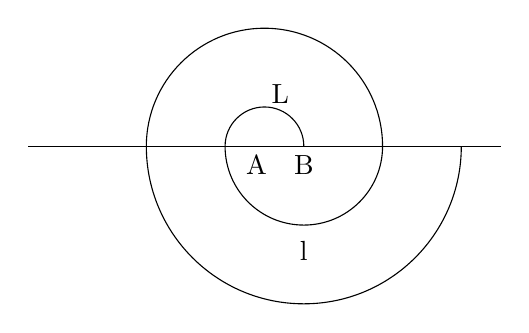
\begin{tikzpicture}

% Define the centers A and B
\coordinate (A) at (0,0);
\coordinate (B) at (0.5,0);

% Draw the spiral using semicircles
\foreach \r in {0.5,1.5} {
  \draw (A) ++(\r,0) arc (0:180:\r);
}
\foreach \r in {1.0,2.0} {
  \draw (B) ++(\r,0) arc (0:-180:\r);
}
\node[label={above:A}] at (-0.1,-0.6){};
\node[label={above:B}] at (0.5,-0.6){};
\node[label={above:l}] at (0.5,-1.7){};
\node[label={above:L}] at (0.2,0.3){};
% Draw the axes (optional)
\draw[-] (-3,0) -- (3,0);

\end{tikzpicture}\\
\solution
\pagebreak

\item 200 logs are stacked in the following manner: 20 logs in the bottom row, 19 in the next row,18 in the row next to it and so on (see Fig \ref{fig:10.5.3.19.q}). In how many rows are the 200 logs placed and how many logs are in the top row?
\begin{figure}[h]
    \centering
    \includegraphics[width=1\linewidth]{ncert-maths/10/5/3/19/figs/question.png}
    \caption{ }
    \label{fig:10.5.3.19.q}
\end{figure}
\solution \iffalse
\let\negmedspace\undefined
\let\negthickspace\undefined
\documentclass[journal,12pt,twocolumn]{IEEEtran}
\usepackage{cite}
\usepackage{amsmath,amssymb,amsfonts,amsthm}
\usepackage{algorithmic}
\usepackage{graphicx}
\usepackage{textcomp}
\usepackage{xcolor}
\usepackage{txfonts}
\usepackage{listings}
\usepackage{enumitem}
\usepackage{mathtools}
\usepackage{gensymb}
\usepackage{comment}
\usepackage[breaklinks=true]{hyperref}
\usepackage{tkz-euclide} 
\usepackage{listings}
\usepackage{gvv}                                        
\def\inputGnumericTable{}                                 
\usepackage[latin1]{inputenc}                                
\usepackage{color}                                            
\usepackage{array}                                            
\usepackage{longtable}                                       
\usepackage{calc}                                             
\usepackage{multirow}                                         
\usepackage{hhline}                                           
\usepackage{ifthen}                                           
\usepackage{lscape}

\newtheorem{theorem}{Theorem}[section]
\newtheorem{problem}{Problem}
\newtheorem{proposition}{Proposition}[section]
\newtheorem{lemma}{Lemma}[section]
\newtheorem{corollary}[theorem]{Corollary}
\newtheorem{example}{Example}[section]
\newtheorem{definition}[problem]{Definition}
\newcommand{\BEQA}{\begin{eqnarray}}
\newcommand{\EEQA}{\end{eqnarray}}
\newcommand{\define}{\stackrel{\triangle}{=}}
\theoremstyle{remark}
\newtheorem{rem}{Remark}
\begin{document}

\bibliographystyle{IEEEtran}
\vspace{3cm}

\title{10.5.3.19}
\author{EE23BTECH11065 - prem sagar}
\maketitle
\newpage

\bigskip 

\renewcommand{\thefigure}{\arabic{figure}}
\renewcommand{\thetable}{\arabic{table}}
\textbf{Question}:\\  200 logs are stacked in the following manner: 20 logs in the bottom row, 19 in the next row,18 in the row next to it and so on (see Fig \ref{fig:10.5.3.19.q}). In how many rows are the 200 logs placed and how many logs are in the top row?
\begin{figure}[h]
    \centering
    \includegraphics[width=1\linewidth]{ncert-maths/10/5/3/19/figs/question.png}
    \caption{ }
    \label{fig:10.5.3.19.q}
\end{figure}
\fi
\\\\\textbf{Solution}:
\begin{table}[!ht]
  \def\arraystretch{1.5}
  \centering
  \renewcommand\thetable{1}
  \begin{tabular}{|c|c|c|}
   \hline
   \textbf{Symbol} & \textbf{Value}& \textbf{Description} \\
   \hline
        $ x\brak{0}$ & $20$ & first term of AP\\
        \hline
        d & ${-1}$ & common difference\\
        \hline
        $x\brak{n}$ &  & $\brak{x\brak{0}+nd}u\brak{n}$\\
        \hline
        $y\brak{n}$ & $200$ & \\
        \hline
\end{tabular}

  \caption{input parameters}
  \label{tab:10.5.3.19}
  \end{table}
\\\\by the differentiation property:
\\\begin{align}
 x\brak{n}\overset{z}{\longleftrightarrow} (-z)\frac{dX\brak{z}}{dz}
 \\\implies n u\brak{n}\overset{z}{\longleftrightarrow} \frac{z^{-1}}{\brak{1-z^{-1}}^2},\abs z>1
 \label{eq:10.5.3.19.2}
 \\\implies n^2 u\brak{n}\overset{z}{\longleftrightarrow} \frac{z^{-1}\brak{z^{-1}+1}}{\brak{1-z^{-1}}^3} ,\abs z>1
 \end{align}
 \begin{align}
 \implies Z^{-1}\biggl[\frac{1}{\brak{1-z^{-1}}^2}\biggr]&=\brak{n+1}u\brak{n}
 \label{eq:10.5.3.19.4}
\\\implies Z^{-1}\biggl[\frac{z^{-1}}{\brak{1-z^{-1}}^3}\biggr]&=\frac{n\brak{n+1}}{2}u\brak{n}
\label{eq:10.5.3.19.5}
 \end{align}
 from \eqref{eq:10.5.3.19.2}
\begin{align} 
\implies X\brak{Z}&=\frac{20}{1-z^{-1}}-\frac{z^{-1}}{\brak{1-z^{-1}}^2}\,,\abs{z}>1
\label{eq:10.5.3.19.9}
\end{align}
from \eqref{eq:10.5.3.19.9}
\begin{align}
y\brak{n}&=x\brak{n}*u\brak{n}
\\\implies Y\brak{Z}&=X\brak{Z}U\brak{Z}
\\&=\frac{20}{\brak{1-z^{-1}}^2}-\frac{z^{-1}}{\brak{1-z^{-1}}^3}\,,\abs{z}>1
\end{align}
substituting \eqref{eq:10.5.3.19.4}, \eqref{eq:10.5.3.19.5}:
\begin{align}
y\brak{n}&=\brak{20\brak{n+1}-\frac{n\brak{n+1}}{2}}u\brak{n}
\\&=\frac{\brak{n+1}\brak{40-n}}{2}
\end{align}
since number of logs=200
\begin{align}
 200&=\frac{\brak{n+1}\brak{40-n}}{2}   
\\n&=24,15
\end{align}
\\for n=24
\begin{align}
x\brak{24}&=20-24
\\&={-4}
\end{align}
but logs can't be negative
\\for n=15
\begin{align}
x\brak{15}&=20-15
\\&=5
\end{align}
\\so number of rows=15
\\number of logs=5
\\\begin{figure}[h]
  \renewcommand\thefigure{1}
    \centering
    \includegraphics[width=1\linewidth]{ncert-maths/10/5/3/19/figs/figure_plot.png}
    \caption{plot of y\brak{n} v/s n}
\end{figure}

\pagebreak

\item In an AP:
\begin{enumerate}
\item given a = 5, d = 3,$a_n=5$, find n and $S_n$.
\item given a = 7, $a_{13}$=35, find d and $S_{13}$.
\item given $a_{12}=37$, d = 3, find a and $S_{12}$.
\item given $a_3$= 15, $S_{10}$ = 125, find d and $a_{10}$.
\item given d = 5, $S_9$= 75, find a and $a_9$.
\item given a = 2, d = 8, $S_n$= 90, find n and $a_n$.
\item given a = 8, $a_n$= 62, $S_n$= 210, find n and d.
\item given an= 4, d = 2, $S_n=-14$, find n and a.
\item given a = 3, n = 8, S = 192, find d.
\item given l = 28, S = 144, and there are total 9 terms. Find a.\\
\end{enumerate}
\solution
\pagebreak

\item Find the sum of n terms of the series:
$1\times2+2\times3+3\times4+4\times5+....$\\
\solution
\pagebreak
\item Find the sum of the first 22 terms of an AP in which $d = 7$ and the $22^{nd}$ term is 149.\\
\solution
\pagebreak

\item Find the sum of integers from 1 to 100 that are divisible by 2 or 5.\\
\solution
\pagebreak

\item In a school, students thought of planting trees in and around the school to reduce air

pollution. It was decided that the number of trees, that each section of each class will

plant, will be the same as the class, in which they are studying, e.g., a section of Class I

will plant 1 tree, a section of Class II will plant 2 trees and so on till Class XII. There are

three sections of each class. How many trees will be planted by the students?\\
\solution
\pagebreak
\end{enumerate}

\chapter{Laplace Transform}
\begin{enumerate}[label=\thesection.\arabic*,ref=\thesection.\theenumi]
\item You are riding in an automobile of mass 3000 kg. Assuming that you are examining the oscillation characteristics of its suspension system. The suspension sags 15 cm when the entire automobile is placed on it. Also, the amplitude of oscillation decreases by 50\% during one complete oscillation. Estimate the values of
\begin{enumerate}[label=(\alph*)]
    \item The spring constant \( K \)
    \item The damping constant \( b \) for the spring and shock absorber system of one wheel, assuming that each wheel supports 750 kg.
\end{enumerate}
\solution
\iffalse
\let\negmedspace\undefined
\let\negthickspace\undefined
\documentclass[journal,12pt,twocolumn]{IEEEtran}
\usepackage{cite}
\usepackage{amsmath,amssymb,amsfonts,amsthm}
\usepackage{algorithmic}
\usepackage{graphicx}
\usepackage{textcomp}
\usepackage{xcolor}
\usepackage{txfonts}
\usepackage{listings}
\usepackage{enumitem}
\usepackage{mathtools}
\usepackage{gensymb}
\usepackage{comment}
\usepackage[breaklinks=true]{hyperref}
\usepackage{tkz-euclide}
\usepackage{listings}
\usepackage{gvv}
\def\inputGnumericTable{}
\usepackage[latin1]{inputenc}
\usepackage{color}
\usepackage{array}
\usepackage{longtable}
\usepackage{calc}
\usepackage{multirow}
\usepackage{hhline}
\usepackage{ifthen}
\usepackage{lscape}
\usepackage{float}

\newtheorem{theorem}{Theorem}[section]
\newtheorem{problem}{Problem}
\newtheorem{proposition}{Proposition}[section]
\newtheorem{lemma}{Lemma}[section]
\newtheorem{corollary}[theorem]{Corollary}
\newtheorem{example}{Example}[section]
\newtheorem{definition}[problem]{Definition}
\newcommand{\BEQA}{\begin{eqnarray}}
\newcommand{\EEQA}{\end{eqnarray}}
\newcommand{\define}{\stackrel{\triangle}{=}}
\theoremstyle{remark}
\newtheorem{rem}{Remark}
\begin{document}

\bibliographystyle{IEEEtran}
\vspace{3cm}

\title{ANALOG}
\author{EE23BTECH11006 - Ameen Aazam$^{*}$% <-this % stops a space
}
\maketitle
\newpage
\bigskip

\renewcommand{\thefigure}{\theenumi}
\renewcommand{\thetable}{\theenumi}

\vspace{3cm}
\textbf{Question :}
You are riding in an automobile of mass 3000 kg. Assuming that you are examining the oscillation characteristics of its suspension system. The suspension sags 15 cm when the entire automobile is placed on it. Also, the amplitude of oscillation decreases by 50\% during one complete oscillation. Estimate the values of
\begin{enumerate}[label=(\alph*)]
    \item The spring constant \( K \)
    \item The damping constant \( b \) for the spring and shock absorber system of one wheel, assuming that each wheel supports 750 kg.
\end{enumerate}
\solution
\fi
The parameters are :
    \begin{table}[htbp]
        \centering
        \begin{tabular}{|l|l|l|}
\hline
\textbf{Parameter} & \textbf{Value(SI)} & \textbf{Description} \\ \hline
$x_{0}$ & 0.15 & Initial spring compression \\ \hline
$m$          & 750 & Mass              \\ \hline
$g$          & 9.8 & Gravitational acc \\ \hline
$k$          & $mg/x_{0}$ & Spring constant   \\ \hline
$b$          &  & Damping constant  \\ \hline
\end{tabular}

        \vspace{5pt}
        \caption{Input Parameters}
        \label{tab:Table 1}
    \end{table}
    \begin{table}[htbp]
        \centering
	\begin{tabular}{|l|l|l|}
\hline
\textbf{Parameter} & \textbf{Value(SI)} & \textbf{Description} \\ \hline
$x$          &  & Spring Extension \\ \hline
$F_1$ & $kx$ & Spring Force \\ \hline
$F_2$ & $b\frac{dx}{dt}$ & Damping Force \\ \hline
$s$ & & Complex Frequency \\ \hline
$s_1, s_2$          &  & Values of s \\ \hline
\end{tabular}

        \vspace{5pt}
        \caption{Intermediate Parameters}
        \label{tab:Table 2}
    \end{table}
    
    \vspace{15pt}
    


    Initially the automobile is in rest, so we can use,
    \begin{align}
        &mg = kx_0 \label{eq:1}\\
        \implies &k=\frac{mg}{x_0} \label{eq:2}
    \end{align}

    \begin{figure}[h]
        \centering
        \includegraphics[width=0.5\columnwidth]{ncert-physics/11/14/figs/11_14_21_fbd.pdf}
        \caption{FBD of the damped oscillation system}
        \label{fig:Fig-1}
    \end{figure}

    Now, as the oscillation begins, from the \figref{fig:Fig-1} we net force on the mass as,
    \begin{align}
        &F=F_{1}+F_{2}+mgu(t) \label{eq:3}\\
        \implies &-m\frac{d^2x(t)}{dt^2}=kx(t)+b\frac{dx(t)}{dt}+mgu(t) \label{eq:4}\\
        \implies &\frac{d^2x(t)}{dt^2}+\brak{\frac{b}{m}}\frac{dx(t)}{dt}+\brak{\frac{k}{m}}x(t)=-gu(t) \label{eq:5}
    \end{align}

    Now, taking the Laplace transform on both sides,
    \begin{align}
        &s^2X(s)+\frac{b}{m}sX(s)+\frac{k}{m}X(s)=-\frac{g}{s} \label{eq:6}\\
        \implies &X(s)=-\frac{g}{s\brak{s^2+\frac{b}{m}s+\frac{k}{m}}} \label{eq:7}\\
        \implies &X(s)=-\frac{g}{s(s-s_1)(s-s_2)} \label{eq:8}
    \end{align}
    Where
    \begin{align}
        &s_1=-\frac{b}{2m}+\sqrt{\brak{\frac{b}{2m}}^2-\frac{k}{m}} \label{eq:9}\\
        &s_2=-\frac{b}{2m}-\sqrt{\brak{\frac{b}{2m}}^2-\frac{k}{m}} \label{eq:10}
    \end{align}
    From \eqref{eq:8} we get,
    \begin{align}
        \begin{split}
            \implies &X(s)=\frac{g}{(s_1-s_2)}\sbrak{\frac{1}{s_2(s-s_2)}-\frac{1}{s_1(s-s_1)}} \\
            &+\frac{g}{s_1s_2}\brak{\frac{1}{s}} \label{eq:11}
        \end{split}
    \end{align}
    Now again taking the inverse Laplace transform we have,
    \begin{align}
        &x(t)=\frac{g}{s_1s_2}u(t)+\frac{g}{(s_1-s_2)}\sbrak{\frac{1}{s_2}e^{s_2t}-\frac{1}{s_1}e^{s_1t}}u(t)\label{eq:12}
    \end{align}
    \begin{align}
    \begin{split}
    \implies &x(t) =\sqrt{\brak{\frac{mg}{k}}^2 + \brak{\frac{gb}{2mk}}^2}e^{-bt/2m}u(t) \\
            &\sin{\brak{\sqrt{\frac{k}{m} - \brak{\frac{b}{2m}}^2}t + \tan^{-1}\brak{\frac{2mg\sqrt{\frac{k}{m} - \brak{\frac{b}{2m}}^2}}{gb}}}} \\
            &+ \frac{mg}{k}
        u(t) \label{eq:13}
\end{split}
\end{align}
    (Substituting the values of $s_1$ and $s_2$ from \eqref{eq:9} and \eqref{eq:10})

    From \eqref{eq:13} we have the amplitude after one time period $T$,
    \begin{align}
        \begin{split}
            &\frac{1}{2}\sqrt{\brak{\frac{mg}{k}}^2+\brak{\frac{gb}{2mk}}^2}= \\
            &\sqrt{\brak{\frac{mg}{k}}^2+\brak{\frac{gb}{2mk}}^2}e^{-bT/2m} \label{eq:14}
        \end{split}
    \end{align}
    \begin{align}
        \implies &e^{\pi b/\sqrt{mk}}=2 \label{eq:15}\\
        \implies &b=\frac{\sqrt{mk}\ln{2}}{\pi} \label{eq:16}
    \end{align}
    \begin{figure}[h]
        \centering
        \includegraphics[width=0.8\columnwidth]{ncert-physics/11/14/figs/11.14.21_plot.png}
        \caption{Displacement Vs. Time Graph}
        \label{fig:Fig-2}
    \end{figure}

%\end{document}

\pagebreak

\item A mass attached to a spring is free to oscillate, with angular velocity $\omega$, in a horizontal
plane without friction or damping. It is pulled to a distance $x_0$
 and pushed towards
the centre with a velocity $v_0$
 at time t = 0. Determine the amplitude of the resulting
oscillations in terms of the parameters $\omega{}$, $x_0$,
 and $v_0$
. [Hint : Start with the equation
$x = a \cos\brak{\omega{t}+\theta{}}$ and note that the initial velocity is negative.]\\
\solution
\pagebreak
\end{enumerate}

\chapter{Systems}
\begin{enumerate}[label=\thesection.\arabic*,ref=\thesection.\theenumi]
\item A simple pendulum of length $l$ and having a bob of mass $M$ is suspended in a car. The car is moving in a circular track of radius $R$ with a uniform speed $v$. If the pendulum makes small oscillations in a radial direction about its equilibrium position, what will be its time period?
\pagebreak
\item A spring balance has a scale that that reads from $0$ to $50$ kg.The length of the scale is 20 cm.A body is suspended from this balance,when displaced and released, oscillates with a period of 0.6 s.What is weight of the body? 
\pagebreak
\end{enumerate}

\backmatter
\appendix
\chapter{ Convolution}
\begin{enumerate}[label=\thechapter.\arabic*,ref=\thechapter.\theenumi]
\numberwithin{equation}{enumi}
\numberwithin{figure}{enumi}
\numberwithin{table}{enumi}

\item The convolution sum is defined as
\begin{align}
	y(n) &= x(n)* h(n) = \sum_{k=-\infty}^{\infty}x\brak{k}h\brak{n-k}
	\label{eq:conv}
\end{align}
\item The unit step function is defined as
\begin{align}
	u(n) = 
	\begin{cases}
		1 & n \ge 0
		\\
		0 & \text{otherwise}
	\end{cases}
	\label{eq:unit-step}
\end{align}
\item If 
\begin{align}
	x(n) = 0, \quad n < 0, 
\end{align}
from 
	\eqref{eq:conv},
\begin{align}
	x(n)*u(n)  = \sum_{k=0}^{n}x\brak{k}
	\label{eq:conv-sum}
\end{align}
\end{enumerate}

\chapter{ Z-transform}
\begin{enumerate}[label=\thechapter.\arabic*,ref=\thechapter.\theenumi]
\numberwithin{equation}{enumi}
\numberwithin{figure}{enumi}
\numberwithin{table}{enumi}
\item 
	The $Z$-transform of $p(n)$ is defined as
\begin{align}
P(z) = \sum_{n=-\infty}^{\infty}p(n)z^{-n}
\label{eq:ztrans}
\end{align}
\item If 
\begin{align}
	p(n) &= p_1(n)* p_2(n),
	\\
	P(z)&=P_1(z)P_2(z)
\end{align}
The above property follows from Fourier analysis and is fundamental to signal processing. 
\item For a Geometric progression 
\begin{align}
	x\brak{n} &=x\brak{0}r^nu\brak{n},
	\\
         \implies      X\brak{z} &= \sum_{n=-\infty}^{\infty}x\brak{n}z^{-n}
               =\sum_{n=0}^{\infty}x\brak{0}r^nz^{-n}\\
                &=\sum_{n=0}^{\infty}x\brak{0}\brak{rz^{-1}}^n\\
               &= \frac{x\brak{0}}{1-rz^{-1}}, \quad \abs{z}>\abs{r} 
	       \label{eq:gpz}
\end{align}
\item Let 
\begin{align}
	u(n) = 
	\begin{cases}
		1 & n \ge 0
		\\
		0 & \text{otherwise}
	\end{cases}
\end{align}
	       Substituting $r = 1$ in \eqref{eq:gpz},
\begin{align}
	u(n) \system{Z}	U(z) = 
                \frac{1}{1-z^{-1}}, \quad \abs{z}>1
	       \label{eq:uz}
\end{align}
\item From 
\eqref{eq:ztrans}
	       and 
	       \eqref{eq:uz},
\begin{align}
	U(z) &= \sum_{n = -\infty}^{\infty} u(n) z^{-n} 
	\\
\implies	\frac{dU(z)}{dz} &= -{z}^{-1} \sum_{n = -\infty}^{\infty} nu(n) z^{-n}\\
\therefore	nu(n) &\system{Z}\frac{z^{-1}}{(1-z^{-1})^{2}}, \quad \abs{z} > 1 
	       \label{eq:uzder}
\end{align}
\item For an AP, 
\begin{align}
	x(n) &= \sbrak{x(0) + nd} u(n) = x(0)u(n) + dnu(n)  \\
	\implies X(z) &= \frac{x(0)}{1-z^{-1}} + \frac{dz^{-1}}{(1-z^{-1})^{2}}, \quad \abs{z} > 1 
	       \label{eq:apz}
\end{align}
upon substituting from 
	       \eqref{eq:uz}
	       and
	       \eqref{eq:uzder}.
\item General form of GP
\begin{align}
	x\brak{n}&=x\brak{0}r^n u\brak{n} \label{eq:appendixGPGeneralform}
\end{align}
Let 
\begin{align}
	y\brak{n} &=x\brak{n} * u\brak{n} \label{eq:convolutionSum}\\
	&=\sum _{k=-\infty}^{\infty} x\brak{k} u\brak{n-k}
\end{align}
on substituting \eqref{eq:appendixGPGeneralform} in The convolution sum 
\begin{align}
	y\brak{n} &= \sum_{k=-\infty}^{\infty} x\brak{0}r^n u\brak{n} u\brak{n-k}\\
	&= \sum _{k=0}^{n} x\brak{0} r^n
\end{align}
Which gives us sum of GP, So On Taking Z-Transform on \eqref{eq:convolutionSum}
\begin{align}
	Y\brak{z}&= X\brak{z} U\brak{z}
\end{align}
From Z-Transform of a term in GP 
\begin{align}
	X\brak{z}&=	\frac{x\brak{0}}{1-rz^{-1}}  \label{eq:GPTransform} \quad \abs{z} > \abs{r}
\end{align}
and Z-Transform of unit step is 
\begin{align}
	U\brak{z} &=\frac{1}{1-z^{-1}}  \quad \abs{z^{-1}}<1\\
	\implies Y\brak{z}&=\brak{\frac{x\brak{0}}{1-rz^{-1}}}\brak{\frac{1}{1-z^{-1}}} \quad \abs{z} > \abs{r} \quad \text{and}  \quad \abs{z}>\abs{1}
\end{align}
By using Partial Fractions
\begin{align}
	Y\brak{z}&=x\brak{0}\brak{\frac{A}{1-rz^{-1}} + \frac{B}{1-z^{-1}}}\\
	A&=\frac{r}{r-1}\\
	B&= \frac{-1}{r-1}
\end{align}
Using \eqref{eq:GPTransform} and Taking inverse Z-transform 
\begin{align}
	y\brak{n}&=\frac{x\brak{0}}{r-1}\brak{r\brak{r^n}-1}u\brak{n}\\
	&=x\brak{0}\brak{\frac{r^{n+1}-1}{r-1}}u\brak{n}
\end{align}
\end{enumerate}

\chapter{Contour Integration}
\begin{enumerate}[label=\thechapter.\arabic*,ref=\thechapter.\theenumi]
\numberwithin{equation}{enumi}
\numberwithin{figure}{enumi}
\numberwithin{table}{enumi}
\item 
\begin{align}
    x\brak{n}          & \xrightarrow{\text{Z}} X\brak{z}             \\
    \implies X\brak{z} & = \sum_{k=-\infty}^{\infty} x\brak{k} z^{-k}
\end{align}
Multiplying both side with $z^{k-1}$ and integrating on a contour integral enclosing the region of convergence. Where $C$ is a counter-clockwise closed contour in region of convergence.
\begin{align}
    \frac{1}{2\pi j} \oint_C X\brak{z} z^{k-1}  dz & = \frac{1}{2\pi j} \oint_C \sum_{k=-\infty}^{\infty} x\brak{k} z^{-n+k-1} dz                               \\
                                                   & =\sum_{k=-\infty}^{\infty} x\brak{k}  \frac{1}{2\pi j} \oint_C z^{-n+k-1} .dz \label{eq:cauchyintegraleq1}
\end{align}
From cauchy's integral theorem
\begin{align}
    \frac{1}{2\pi j} \oint_C z^{-k} dz & = \begin{cases}
                                               1, \quad k = 1 \\
                                               0, \quad k\neq 1
                                           \end{cases}  \\
                                       & = \delta\brak{1-k}
\end{align}
So eq \eqref{eq:cauchyintegraleq1} becomes
\begin{align}
    \frac{1}{2\pi j} \oint_C X\brak{z} z^{k-1} dz & = \sum_{k=-\infty}^{\infty} x\brak{k} \delta \brak{k-n}                       \\
    \implies x\brak{n}                            & =  \frac{1}{2\pi j} \oint_C X\brak{z} z^{n-1} dz \label{eq:cauchyintegraleq2}
\end{align}
Contour integrals like \eqref{eq:cauchyintegraleq2} can be evaluated using Cauchy's residue theorem.
\begin{align}
    x\brak{n} & =  \frac{1}{2\pi j} \oint_C X\brak{z} z^{n-1} dz                               \\
              & = \sum \sbrak{\text{Residue of } X\brak{z} z^{n-1} \text{ at poles inside } C}
\end{align}

\end{enumerate}

\chapter{Fourier Series}
\begin{enumerate}[label=\thechapter.\arabic*,ref=\thechapter.\theenumi]
\numberwithin{equation}{enumi}
\numberwithin{figure}{enumi}
\numberwithin{table}{enumi}

\item Complex Fourier Series\\
Consider,
\begin{align}
	x(t) &= \sum_{n=-\infty}^{\infty} c_{n}e^{j2\pi nft}
	\label{eq:compfs}
\end{align}
where $c_{n}$ is the exponential fourier coefficient.
\begin{align}
        c_{n} &= \frac{1}{T} \int_{0}^{T} x(t) e^{-j2\pi nft} \, dt
\end{align}
where $T$ is the time period of function $x(t)$.
\item Trigonometric Fourier Series\\
We can write:
\begin{align}
	e^{j2\pi nft} = cos(2\pi nft t) + j sin(2\pi nft)
	\label{eq:expfs}
\end{align}
Substituting \eqref{eq:expfs} in \eqref{eq:compfs}
\begin{align}
	 x(t) &= \sum_{n=-\infty}^{\infty} c_{n} \brak{\cos(2\pi nft) + j \sin(2\pi nft)}\\
	      &= a_0 + \sum_{n=1}^{\infty} \brak{a_{n} \cos(2\pi nft)} + \brak{b_{n} \sin(2\pi nft)}
\end{align}
where $a_0, a_{n}$ and $b_{n}$ are trigonometric fourier series.
\begin{align}
          a_{0} &= c_{0}\\
                &=\frac{1}{T} \int_{0}^{T} x(t) \, dt\\
          a_{n} &= 2Re(c_{n})\\
                &=\frac{2}{T} \int_{0}^{T} x(t)\cos(2\pi nft) \, dt\\
          b_{n} &= -2Im(c_{n})\\
                &= \frac{2}{T} \int_{0}^{T} x(t)\sin(2\pi nft) \, dt
\end{align}
\end{enumerate}


\latexprintindex
\end{document}

 
